\documentclass[twoside]{book}

% Packages required by doxygen
\usepackage{calc}
\usepackage{doxygen}
\usepackage{graphicx}
\usepackage[utf8]{inputenc}
\usepackage{makeidx}
\usepackage{multicol}
\usepackage{multirow}
\usepackage{textcomp}
\usepackage[table]{xcolor}

% Font selection
\usepackage[T1]{fontenc}
\usepackage{mathptmx}
\usepackage[scaled=.90]{helvet}
\usepackage{courier}
\usepackage{amssymb}
\usepackage{sectsty}
\renewcommand{\familydefault}{\sfdefault}
\allsectionsfont{%
  \fontseries{bc}\selectfont%
  \color{darkgray}%
}
\renewcommand{\DoxyLabelFont}{%
  \fontseries{bc}\selectfont%
  \color{darkgray}%
}

% Page & text layout
\usepackage{geometry}
\geometry{%
  a4paper,%
  top=2.5cm,%
  bottom=2.5cm,%
  left=2.5cm,%
  right=2.5cm%
}
\tolerance=750
\hfuzz=15pt
\hbadness=750
\setlength{\emergencystretch}{15pt}
\setlength{\parindent}{0cm}
\setlength{\parskip}{0.2cm}
\makeatletter
\renewcommand{\paragraph}{%
  \@startsection{paragraph}{4}{0ex}{-1.0ex}{1.0ex}{%
    \normalfont\normalsize\bfseries\SS@parafont%
  }%
}
\renewcommand{\subparagraph}{%
  \@startsection{subparagraph}{5}{0ex}{-1.0ex}{1.0ex}{%
    \normalfont\normalsize\bfseries\SS@subparafont%
  }%
}
\makeatother

% Headers & footers
\usepackage{fancyhdr}
\pagestyle{fancyplain}
\fancyhead[LE]{\fancyplain{}{\bfseries\thepage}}
\fancyhead[CE]{\fancyplain{}{}}
\fancyhead[RE]{\fancyplain{}{\bfseries\leftmark}}
\fancyhead[LO]{\fancyplain{}{\bfseries\rightmark}}
\fancyhead[CO]{\fancyplain{}{}}
\fancyhead[RO]{\fancyplain{}{\bfseries\thepage}}
\fancyfoot[LE]{\fancyplain{}{}}
\fancyfoot[CE]{\fancyplain{}{}}
\fancyfoot[RE]{\fancyplain{}{\bfseries\scriptsize Generated on Fri Nov 6 2015 15\-:30\-:10 for Optimal Partition by Doxygen }}
\fancyfoot[LO]{\fancyplain{}{\bfseries\scriptsize Generated on Fri Nov 6 2015 15\-:30\-:10 for Optimal Partition by Doxygen }}
\fancyfoot[CO]{\fancyplain{}{}}
\fancyfoot[RO]{\fancyplain{}{}}
\renewcommand{\footrulewidth}{0.4pt}
\renewcommand{\chaptermark}[1]{%
  \markboth{#1}{}%
}
\renewcommand{\sectionmark}[1]{%
  \markright{\thesection\ #1}%
}

% Indices & bibliography
\usepackage{natbib}
\usepackage[titles]{tocloft}
\setcounter{tocdepth}{3}
\setcounter{secnumdepth}{5}
\makeindex

% Hyperlinks (required, but should be loaded last)
\usepackage{ifpdf}
\ifpdf
  \usepackage[pdftex,pagebackref=true]{hyperref}
\else
  \usepackage[ps2pdf,pagebackref=true]{hyperref}
\fi
\hypersetup{%
  colorlinks=true,%
  linkcolor=blue,%
  citecolor=blue,%
  unicode%
}

% Custom commands
\newcommand{\clearemptydoublepage}{%
  \newpage{\pagestyle{empty}\cleardoublepage}%
}


%===== C O N T E N T S =====

\begin{document}

% Titlepage & ToC
\hypersetup{pageanchor=false}
\pagenumbering{roman}
\begin{titlepage}
\vspace*{7cm}
\begin{center}%
{\Large Optimal Partition }\\
\vspace*{1cm}
{\large Generated by Doxygen 1.8.6}\\
\vspace*{0.5cm}
{\small Fri Nov 6 2015 15:30:10}\\
\end{center}
\end{titlepage}
\clearemptydoublepage
\tableofcontents
\clearemptydoublepage
\pagenumbering{arabic}
\hypersetup{pageanchor=true}

%--- Begin generated contents ---
\chapter{Hierarchical Index}
\section{Class Hierarchy}
This inheritance list is sorted roughly, but not completely, alphabetically\-:\begin{DoxyCompactList}
\item \contentsline{section}{Abstract\-Set}{\pageref{classAbstractSet}}{}
\begin{DoxyCompactList}
\item \contentsline{section}{Bi\-Set}{\pageref{classBiSet}}{}
\item \contentsline{section}{Graph}{\pageref{classGraph}}{}
\begin{DoxyCompactList}
\item \contentsline{section}{Complete\-Graph}{\pageref{classCompleteGraph}}{}
\item \contentsline{section}{Filiform\-Graph}{\pageref{classFiliformGraph}}{}
\item \contentsline{section}{Random\-Graph}{\pageref{classRandomGraph}}{}
\item \contentsline{section}{Ring\-Graph}{\pageref{classRingGraph}}{}
\end{DoxyCompactList}
\item \contentsline{section}{Hierarchical\-Hierarchical\-Set}{\pageref{classHierarchicalHierarchicalSet}}{}
\item \contentsline{section}{Hierarchical\-Ordered\-Set}{\pageref{classHierarchicalOrderedSet}}{}
\item \contentsline{section}{Hierarchical\-Set}{\pageref{classHierarchicalSet}}{}
\item \contentsline{section}{Multi\-Set}{\pageref{classMultiSet}}{}
\item \contentsline{section}{N\-H\-O\-Set}{\pageref{classNHOSet}}{}
\item \contentsline{section}{Nonconstrained\-Ordered\-Set}{\pageref{classNonconstrainedOrderedSet}}{}
\item \contentsline{section}{Nonconstrained\-Set}{\pageref{classNonconstrainedSet}}{}
\item \contentsline{section}{Ordered\-Set}{\pageref{classOrderedSet}}{}
\item \contentsline{section}{Ring}{\pageref{classRing}}{}
\end{DoxyCompactList}
\item \contentsline{section}{Bi\-Subset}{\pageref{classBiSubset}}{}
\item \contentsline{section}{Data\-Point\-Struct}{\pageref{structDataPointStruct}}{}
\item \contentsline{section}{Dataset}{\pageref{classDataset}}{}
\item \contentsline{section}{Datatree}{\pageref{classDatatree}}{}
\item \contentsline{section}{Graph\-Component}{\pageref{classGraphComponent}}{}
\item \contentsline{section}{H\-H\-Node}{\pageref{classHHNode}}{}
\item \contentsline{section}{H\-Node}{\pageref{classHNode}}{}
\item \contentsline{section}{H\-O\-Node}{\pageref{classHONode}}{}
\item \contentsline{section}{Multi\-Subset}{\pageref{classMultiSubset}}{}
\item \contentsline{section}{N\-H\-O\-Node}{\pageref{classNHONode}}{}
\item \contentsline{section}{Objective\-Function}{\pageref{classObjectiveFunction}}{}
\begin{DoxyCompactList}
\item \contentsline{section}{Information\-Bottleneck}{\pageref{classInformationBottleneck}}{}
\item \contentsline{section}{Logarithmic\-Score}{\pageref{classLogarithmicScore}}{}
\item \contentsline{section}{Relative\-Entropy}{\pageref{classRelativeEntropy}}{}
\end{DoxyCompactList}
\item \contentsline{section}{Objective\-Value}{\pageref{classObjectiveValue}}{}
\begin{DoxyCompactList}
\item \contentsline{section}{Bottleneck\-Objective\-Value}{\pageref{classBottleneckObjectiveValue}}{}
\item \contentsline{section}{Logarithmic\-Objective\-Value}{\pageref{classLogarithmicObjectiveValue}}{}
\item \contentsline{section}{Relative\-Objective\-Value}{\pageref{classRelativeObjectiveValue}}{}
\end{DoxyCompactList}
\item \contentsline{section}{Ordered\-Datatree}{\pageref{classOrderedDatatree}}{}
\item \contentsline{section}{Part}{\pageref{classPart}}{}
\begin{DoxyCompactList}
\item \contentsline{section}{Bi\-Part}{\pageref{classBiPart}}{}
\item \contentsline{section}{Multi\-Part}{\pageref{classMultiPart}}{}
\end{DoxyCompactList}
\item \contentsline{section}{Partition}{\pageref{classPartition}}{}
\item \contentsline{section}{Prediction\-Dataset}{\pageref{classPredictionDataset}}{}
\item \contentsline{section}{Timer}{\pageref{classTimer}}{}
\item \contentsline{section}{Tree\-To\-Add}{\pageref{structTreeToAdd}}{}
\item \contentsline{section}{Uni\-Set}{\pageref{classUniSet}}{}
\begin{DoxyCompactList}
\item \contentsline{section}{Hierarchical\-Uni\-Set}{\pageref{classHierarchicalUniSet}}{}
\item \contentsline{section}{Ordered\-Uni\-Set}{\pageref{classOrderedUniSet}}{}
\end{DoxyCompactList}
\item \contentsline{section}{Uni\-Subset}{\pageref{classUniSubset}}{}
\end{DoxyCompactList}

\chapter{Class Index}
\section{Class List}
Here are the classes, structs, unions and interfaces with brief descriptions\-:\begin{DoxyCompactList}
\item\contentsline{section}{\hyperlink{classAbstractSet}{Abstract\-Set} \\*Abstract class defining a set of elements that one wants to partition while optimising some (decomposable) objective and preserving some algebraic constraints (set of feasible parts) }{\pageref{classAbstractSet}}{}
\item\contentsline{section}{\hyperlink{classBinaryTreeUniSet}{Binary\-Tree\-Uni\-Set} \\*A uni-\/dimensional set of elements structured according to a complete binary tree, and such that the feasible subsets are all the nodes of the tree }{\pageref{classBinaryTreeUniSet}}{}
\item\contentsline{section}{\hyperlink{classBiPart}{Bi\-Part} \\*A bi-\/part is a subset of a bi-\/dimensional set of elements (individuals) }{\pageref{classBiPart}}{}
\item\contentsline{section}{\hyperlink{classBiSet}{Bi\-Set} }{\pageref{classBiSet}}{}
\item\contentsline{section}{\hyperlink{classBiSubset}{Bi\-Subset} }{\pageref{classBiSubset}}{}
\item\contentsline{section}{\hyperlink{classBottleneckObjectiveValue}{Bottleneck\-Objective\-Value} }{\pageref{classBottleneckObjectiveValue}}{}
\item\contentsline{section}{\hyperlink{classChainVoterGraph}{Chain\-Voter\-Graph} }{\pageref{classChainVoterGraph}}{}
\item\contentsline{section}{\hyperlink{classCompleteGraph}{Complete\-Graph} }{\pageref{classCompleteGraph}}{}
\item\contentsline{section}{\hyperlink{classCompleteVoterGraph}{Complete\-Voter\-Graph} \\*An interaction graph with edges between each pair of nodes (in both direction, with equal weight for each edge) }{\pageref{classCompleteVoterGraph}}{}
\item\contentsline{section}{\hyperlink{structDataPointStruct}{Data\-Point\-Struct} }{\pageref{structDataPointStruct}}{}
\item\contentsline{section}{\hyperlink{classDataset}{Dataset} }{\pageref{classDataset}}{}
\item\contentsline{section}{\hyperlink{classDatatree}{Datatree} }{\pageref{classDatatree}}{}
\item\contentsline{section}{\hyperlink{classEmptyVoterMeasurement}{Empty\-Voter\-Measurement} \\*A measurement without any probe (no observation) }{\pageref{classEmptyVoterMeasurement}}{}
\item\contentsline{section}{\hyperlink{classFiliformGraph}{Filiform\-Graph} }{\pageref{classFiliformGraph}}{}
\item\contentsline{section}{\hyperlink{structglobalArgs__t}{global\-Args\-\_\-t} }{\pageref{structglobalArgs__t}}{}
\item\contentsline{section}{\hyperlink{classGraph}{Graph} }{\pageref{classGraph}}{}
\item\contentsline{section}{\hyperlink{classGraphBasedUniSet}{Graph\-Based\-Uni\-Set} }{\pageref{classGraphBasedUniSet}}{}
\item\contentsline{section}{\hyperlink{classGraphComponent}{Graph\-Component} }{\pageref{classGraphComponent}}{}
\item\contentsline{section}{\hyperlink{classHHNode}{H\-H\-Node} }{\pageref{classHHNode}}{}
\item\contentsline{section}{\hyperlink{classHierarchicalHierarchicalSet}{Hierarchical\-Hierarchical\-Set} }{\pageref{classHierarchicalHierarchicalSet}}{}
\item\contentsline{section}{\hyperlink{classHierarchicalOrderedSet}{Hierarchical\-Ordered\-Set} }{\pageref{classHierarchicalOrderedSet}}{}
\item\contentsline{section}{\hyperlink{classHierarchicalSet}{Hierarchical\-Set} }{\pageref{classHierarchicalSet}}{}
\item\contentsline{section}{\hyperlink{classHierarchicalUniSet}{Hierarchical\-Uni\-Set} \\*A uni-\/dimensional set of elements structured according to a hierarchy (tree), and such that the feasible subsets are all the nodes of the hierarchy (tree) }{\pageref{classHierarchicalUniSet}}{}
\item\contentsline{section}{\hyperlink{classHNode}{H\-Node} }{\pageref{classHNode}}{}
\item\contentsline{section}{\hyperlink{classHONode}{H\-O\-Node} }{\pageref{classHONode}}{}
\item\contentsline{section}{\hyperlink{classInformationBottleneck}{Information\-Bottleneck} }{\pageref{classInformationBottleneck}}{}
\item\contentsline{section}{\hyperlink{classLogarithmicScore}{Logarithmic\-Score} \\*Class to define and compute the logarithmic score function in the case of point prediction }{\pageref{classLogarithmicScore}}{}
\item\contentsline{section}{\hyperlink{classLogarithmicScoreValue}{Logarithmic\-Score\-Value} }{\pageref{classLogarithmicScoreValue}}{}
\item\contentsline{section}{\hyperlink{classMacroVoterMeasurement}{Macro\-Voter\-Measurement} \\*A measurement consisting in one probe observing all nodes of the interaction graph }{\pageref{classMacroVoterMeasurement}}{}
\item\contentsline{section}{\hyperlink{classMarkovDataSet}{Markov\-Data\-Set} }{\pageref{classMarkovDataSet}}{}
\item\contentsline{section}{\hyperlink{classMarkovProcess}{Markov\-Process} \\*A finite Markov chain described by a discrete state space, an initial distribution, and a transition kernel }{\pageref{classMarkovProcess}}{}
\item\contentsline{section}{\hyperlink{classMarkovTrajectory}{Markov\-Trajectory} }{\pageref{classMarkovTrajectory}}{}
\item\contentsline{section}{\hyperlink{classMicroVoterMeasurement}{Micro\-Voter\-Measurement} \\*A measurement consisting in one probe for each node of the interaction graph }{\pageref{classMicroVoterMeasurement}}{}
\item\contentsline{section}{\hyperlink{classMultiPart}{Multi\-Part} \\*A multi-\/part is a subset of a multi-\/dimensional set of elements (individuals) }{\pageref{classMultiPart}}{}
\item\contentsline{section}{\hyperlink{classMultiSet}{Multi\-Set} \\*A multi-\/dimensional set of elements based on the Cartesian product of several uni-\/dimensional sets (\hyperlink{classUniSet}{Uni\-Set}) and their algebraic structures (feasible subsets and feasible refinements) }{\pageref{classMultiSet}}{}
\item\contentsline{section}{\hyperlink{classMultiSubset}{Multi\-Subset} }{\pageref{classMultiSubset}}{}
\item\contentsline{section}{\hyperlink{classNonconstrainedOrderedSet}{Nonconstrained\-Ordered\-Set} }{\pageref{classNonconstrainedOrderedSet}}{}
\item\contentsline{section}{\hyperlink{classNonconstrainedSet}{Nonconstrained\-Set} }{\pageref{classNonconstrainedSet}}{}
\item\contentsline{section}{\hyperlink{classObjectiveFunction}{Objective\-Function} \\*Abstract class defining an objective function to be associated to a constrained set in order to define the optimisation problem that one wants to solve }{\pageref{classObjectiveFunction}}{}
\item\contentsline{section}{\hyperlink{classObjectiveValue}{Objective\-Value} }{\pageref{classObjectiveValue}}{}
\item\contentsline{section}{\hyperlink{classOrderedDatatree}{Ordered\-Datatree} }{\pageref{classOrderedDatatree}}{}
\item\contentsline{section}{\hyperlink{classOrderedPartition}{Ordered\-Partition} }{\pageref{classOrderedPartition}}{}
\item\contentsline{section}{\hyperlink{classOrderedSet}{Ordered\-Set} }{\pageref{classOrderedSet}}{}
\item\contentsline{section}{\hyperlink{classOrderedUniSet}{Ordered\-Uni\-Set} \\*A uni-\/dimensional set of elements with a total order, and such that the feasible subsets are all the intervals induced by this order }{\pageref{classOrderedUniSet}}{}
\item\contentsline{section}{\hyperlink{classPart}{Part} \\*A part is a subset of a set of elements (individuals) represented by integers }{\pageref{classPart}}{}
\item\contentsline{section}{\hyperlink{classPartition}{Partition} \\*A partition is a collection of pairwise-\/disjoint and covering subsets (parts) of a set of elements }{\pageref{classPartition}}{}
\item\contentsline{section}{\hyperlink{classPredictionDataset}{Prediction\-Dataset} \\*Class to represent a data set for the prediction of a post-\/measurement from the knowledge of a pre-\/measurement (composed of a train set and a test set) }{\pageref{classPredictionDataset}}{}
\item\contentsline{section}{\hyperlink{classQuadraticScore}{Quadratic\-Score} \\*Class to define and compute the quadratic score function in the case of point prediction }{\pageref{classQuadraticScore}}{}
\item\contentsline{section}{\hyperlink{classQuadraticScoreValue}{Quadratic\-Score\-Value} }{\pageref{classQuadraticScoreValue}}{}
\item\contentsline{section}{\hyperlink{classRandomGraph}{Random\-Graph} }{\pageref{classRandomGraph}}{}
\item\contentsline{section}{\hyperlink{classRelativeEntropy}{Relative\-Entropy} }{\pageref{classRelativeEntropy}}{}
\item\contentsline{section}{\hyperlink{classRelativeObjectiveValue}{Relative\-Objective\-Value} }{\pageref{classRelativeObjectiveValue}}{}
\item\contentsline{section}{\hyperlink{classRing}{Ring} }{\pageref{classRing}}{}
\item\contentsline{section}{\hyperlink{classRingGraph}{Ring\-Graph} }{\pageref{classRingGraph}}{}
\item\contentsline{section}{\hyperlink{classTimer}{Timer} }{\pageref{classTimer}}{}
\item\contentsline{section}{\hyperlink{structTreeToAdd}{Tree\-To\-Add} }{\pageref{structTreeToAdd}}{}
\item\contentsline{section}{\hyperlink{classTwoCommunitiesVoterGraph}{Two\-Communities\-Voter\-Graph} \\*An interaction graph consisting in two communities of nodes (complete graph within each community, complete interaction between the two communities, possibly with different weights) }{\pageref{classTwoCommunitiesVoterGraph}}{}
\item\contentsline{section}{\hyperlink{classUnconstrainedUniSet}{Unconstrained\-Uni\-Set} \\*A uni-\/dimensional set of elements with no particular structure, such that all subsets are feasible }{\pageref{classUnconstrainedUniSet}}{}
\item\contentsline{section}{\hyperlink{classUniSet}{Uni\-Set} \\*A uni-\/dimensional set of elements and its algebraic structure (feasible subsets and feasible refinements) }{\pageref{classUniSet}}{}
\item\contentsline{section}{\hyperlink{classUniSubset}{Uni\-Subset} \\*A feasible subset associated to a uni-\/dimensional set of elements (\hyperlink{classUniSet}{Uni\-Set}) }{\pageref{classUniSubset}}{}
\item\contentsline{section}{\hyperlink{classVoterBinning}{Voter\-Binning} }{\pageref{classVoterBinning}}{}
\item\contentsline{section}{\hyperlink{classVoterDataSet}{Voter\-Data\-Set} }{\pageref{classVoterDataSet}}{}
\item\contentsline{section}{\hyperlink{classVoterEdge}{Voter\-Edge} \\*An edge of the interaction graph }{\pageref{classVoterEdge}}{}
\item\contentsline{section}{\hyperlink{classVoterGraph}{Voter\-Graph} \\*The interaction graph describing a Voter Model }{\pageref{classVoterGraph}}{}
\item\contentsline{section}{\hyperlink{classVoterMeasurement}{Voter\-Measurement} \\*A measurement to observe the Voter Model according set of probes }{\pageref{classVoterMeasurement}}{}
\item\contentsline{section}{\hyperlink{classVoterMeasurementState}{Voter\-Measurement\-State} }{\pageref{classVoterMeasurementState}}{}
\item\contentsline{section}{\hyperlink{classVoterMeasurementTrajectory}{Voter\-Measurement\-Trajectory} }{\pageref{classVoterMeasurementTrajectory}}{}
\item\contentsline{section}{\hyperlink{classVoterNode}{Voter\-Node} \\*A node of the interaction graph }{\pageref{classVoterNode}}{}
\item\contentsline{section}{\hyperlink{classVoterProbe}{Voter\-Probe} \\*A probe to observe the Voter Model according to a subset of nodes }{\pageref{classVoterProbe}}{}
\item\contentsline{section}{\hyperlink{classVoterState}{Voter\-State} }{\pageref{classVoterState}}{}
\item\contentsline{section}{\hyperlink{classVoterTrajectory}{Voter\-Trajectory} }{\pageref{classVoterTrajectory}}{}
\end{DoxyCompactList}

\chapter{File Index}
\section{File List}
Here is a list of all documented files with brief descriptions\-:\begin{DoxyCompactList}
\item\contentsline{section}{src/\hyperlink{abstract__set_8hpp}{abstract\-\_\-set.\-hpp} \\*Abstract class defining a set of elements that one wants to partition while optimising some (decomposable) objective and preserving some algebraic constraints (set of feasible parts) }{\pageref{abstract__set_8hpp}}{}
\item\contentsline{section}{src/{\bfseries bi\-\_\-set.\-hpp} }{\pageref{bi__set_8hpp}}{}
\item\contentsline{section}{src/{\bfseries bidimensional\-\_\-relative\-\_\-entropy.\-hpp} }{\pageref{bidimensional__relative__entropy_8hpp}}{}
\item\contentsline{section}{src/{\bfseries check\-\_\-graph\-\_\-datatree.\-hpp} }{\pageref{check__graph__datatree_8hpp}}{}
\item\contentsline{section}{src/{\bfseries csv\-\_\-tools.\-hpp} }{\pageref{csv__tools_8hpp}}{}
\item\contentsline{section}{src/{\bfseries dataset.\-hpp} }{\pageref{dataset_8hpp}}{}
\item\contentsline{section}{src/{\bfseries datatree.\-hpp} }{\pageref{datatree_8hpp}}{}
\item\contentsline{section}{src/{\bfseries geomediatic\-\_\-aggregation.\-hpp} }{\pageref{geomediatic__aggregation_8hpp}}{}
\item\contentsline{section}{src/{\bfseries graph.\-hpp} }{\pageref{graph_8hpp}}{}
\item\contentsline{section}{src/{\bfseries hierarchical\-\_\-hierarchical\-\_\-set.\-hpp} }{\pageref{hierarchical__hierarchical__set_8hpp}}{}
\item\contentsline{section}{src/{\bfseries hierarchical\-\_\-ordered\-\_\-set.\-hpp} }{\pageref{hierarchical__ordered__set_8hpp}}{}
\item\contentsline{section}{src/{\bfseries hierarchical\-\_\-set.\-hpp} }{\pageref{hierarchical__set_8hpp}}{}
\item\contentsline{section}{src/{\bfseries information\-\_\-bottleneck.\-hpp} }{\pageref{information__bottleneck_8hpp}}{}
\item\contentsline{section}{src/\hyperlink{logarithmic__score_8hpp}{logarithmic\-\_\-score.\-hpp} \\*Classes to define and compute the logarithmic score function in the case of point prediction }{\pageref{logarithmic__score_8hpp}}{}
\item\contentsline{section}{src/\hyperlink{markov__process_8hpp}{markov\-\_\-process.\-hpp} \\*Class to build a finite Markov chain }{\pageref{markov__process_8hpp}}{}
\item\contentsline{section}{src/\hyperlink{multi__set_8hpp}{multi\-\_\-set.\-hpp} \\*Classes to represent multi-\/dimensional sets of elements and their algebraic structure (feasible subsets and feasible refinements) }{\pageref{multi__set_8hpp}}{}
\item\contentsline{section}{src/{\bfseries nonconstrained\-\_\-ordered\-\_\-set.\-hpp} }{\pageref{nonconstrained__ordered__set_8hpp}}{}
\item\contentsline{section}{src/{\bfseries nonconstrained\-\_\-set.\-hpp} }{\pageref{nonconstrained__set_8hpp}}{}
\item\contentsline{section}{src/\hyperlink{objective__function_8hpp}{objective\-\_\-function.\-hpp} \\*Abstract class defining an objective function to be associated to a constrained set in order to define the optimisation problem that one wants to solve }{\pageref{objective__function_8hpp}}{}
\item\contentsline{section}{src/{\bfseries optimal\-\_\-partition.\-hpp} }{\pageref{optimal__partition_8hpp}}{}
\item\contentsline{section}{src/{\bfseries orderedset.\-hpp} }{\pageref{orderedset_8hpp}}{}
\item\contentsline{section}{src/{\bfseries partition.\-hpp} }{\pageref{partition_8hpp}}{}
\item\contentsline{section}{src/\hyperlink{prediction__dataset_8hpp}{prediction\-\_\-dataset.\-hpp} \\*Class to represent a data set for the prediction of a post-\/measurement from the knowledge of a pre-\/measurement (composed of a train set and a test set) }{\pageref{prediction__dataset_8hpp}}{}
\item\contentsline{section}{src/{\bfseries prediction\-\_\-programs.\-hpp} }{\pageref{prediction__programs_8hpp}}{}
\item\contentsline{section}{src/{\bfseries programs.\-hpp} }{\pageref{programs_8hpp}}{}
\item\contentsline{section}{src/\hyperlink{quadratic__score_8hpp}{quadratic\-\_\-score.\-hpp} \\*Classes to define and compute the quadratic score function in the case of point prediction }{\pageref{quadratic__score_8hpp}}{}
\item\contentsline{section}{src/{\bfseries relative\-\_\-entropy.\-hpp} }{\pageref{relative__entropy_8hpp}}{}
\item\contentsline{section}{src/{\bfseries ring.\-hpp} }{\pageref{ring_8hpp}}{}
\item\contentsline{section}{src/{\bfseries timer.\-hpp} }{\pageref{timer_8hpp}}{}
\item\contentsline{section}{src/\hyperlink{uni__set_8hpp}{uni\-\_\-set.\-hpp} \\*Some classes to represent uni-\/dimensional sets of elements and their algebraic structure (feasible subsets and feasible refinements) }{\pageref{uni__set_8hpp}}{}
\item\contentsline{section}{src/\hyperlink{voter__graph_8hpp}{voter\-\_\-graph.\-hpp} \\*Classes to build an interaction graph (nodes and edges) describing a Voter Model and some observation tools (probes and measurements) }{\pageref{voter__graph_8hpp}}{}
\end{DoxyCompactList}

\chapter{Class Documentation}
\hypertarget{classAbstractSet}{\section{Abstract\-Set Class Reference}
\label{classAbstractSet}\index{Abstract\-Set@{Abstract\-Set}}
}


Abstract class defining a set of elements that one wants to partition while optimising some (decomposable) objective and preserving some algebraic constraints (set of feasible parts)  




{\ttfamily \#include $<$abstract\-\_\-set.\-hpp$>$}

Inheritance diagram for Abstract\-Set\-:\begin{figure}[H]
\begin{center}
\leavevmode
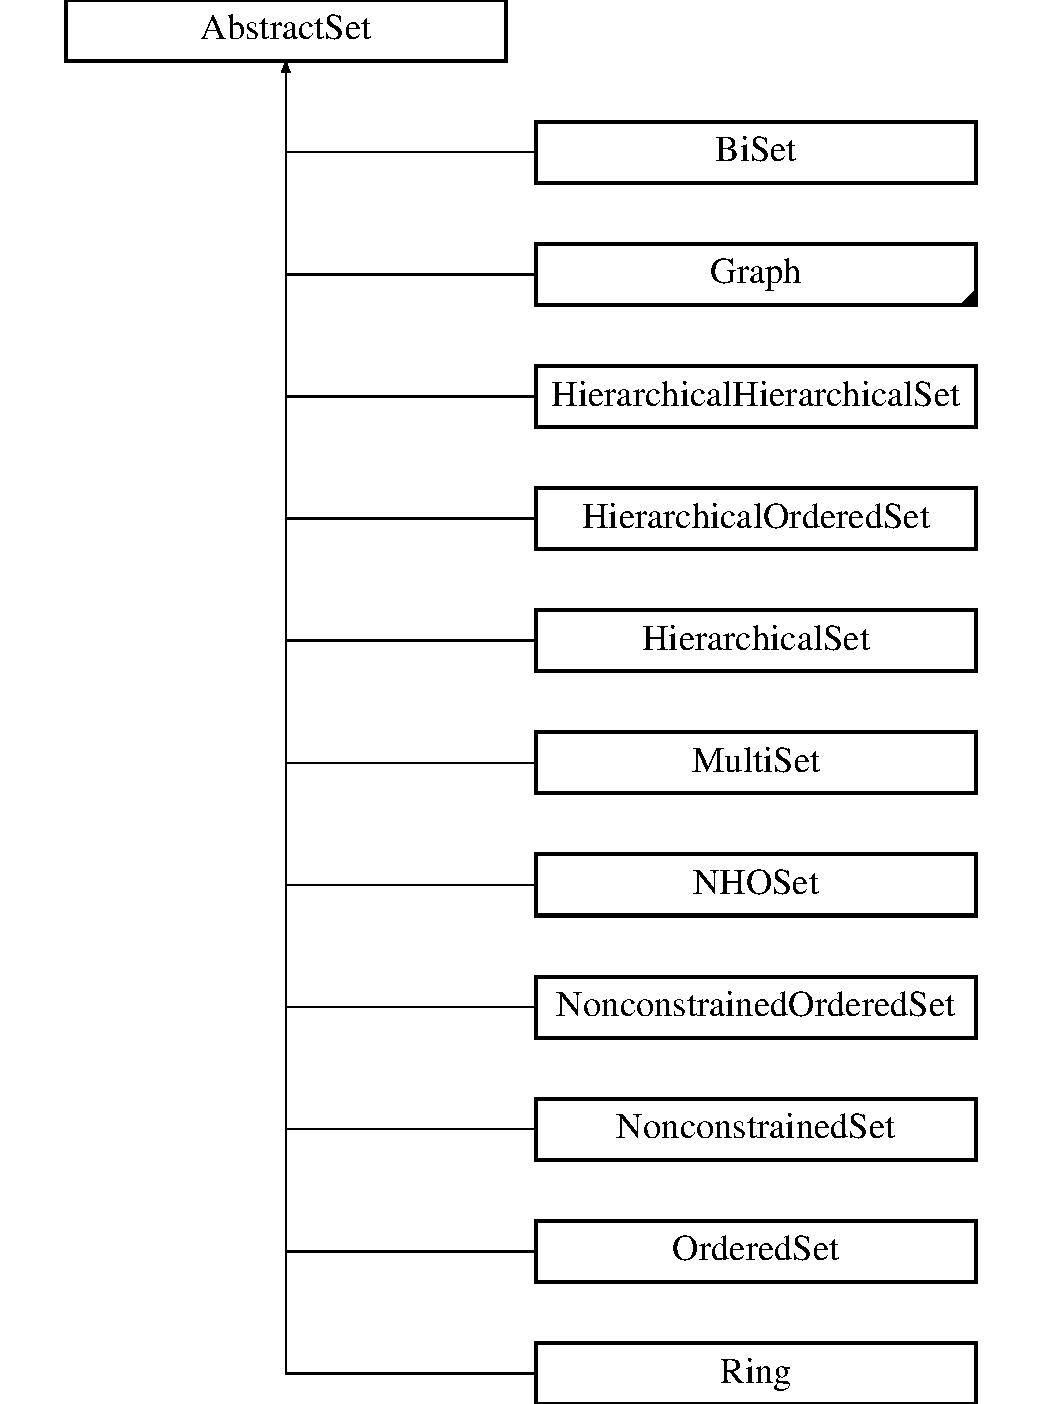
\includegraphics[height=12.000000cm]{classAbstractSet}
\end{center}
\end{figure}
\subsection*{Public Member Functions}
\begin{DoxyCompactItemize}
\item 
virtual \hyperlink{classAbstractSet_adc3db5afd11de63639ddd079ef4ecf45}{$\sim$\-Abstract\-Set} ()
\begin{DoxyCompactList}\small\item\em The objective that one wants to optimise (assumed to be decomposable\-: the objective of a partition is function of the objectives of its parts) \end{DoxyCompactList}\item 
\hypertarget{classAbstractSet_aac0cf2d0ef47c49aa0a7ac393691ff7a}{virtual void \hyperlink{classAbstractSet_aac0cf2d0ef47c49aa0a7ac393691ff7a}{set\-Random} ()=0}\label{classAbstractSet_aac0cf2d0ef47c49aa0a7ac393691ff7a}

\begin{DoxyCompactList}\small\item\em Randomly set the algebraic constraints for quick experiments (warning\-: this method is not always implemented) \end{DoxyCompactList}\item 
\hypertarget{classAbstractSet_a735009927cfae61baa66bbf7b53f76d5}{virtual void \hyperlink{classAbstractSet_a735009927cfae61baa66bbf7b53f76d5}{build\-Data\-Structure} ()=0}\label{classAbstractSet_a735009927cfae61baa66bbf7b53f76d5}

\begin{DoxyCompactList}\small\item\em Build a proper data structure to represent the set and its algebraic constraints (warning\-: this method should always be called after instantiating and parameterising a set, and before calling any other method, such as \hyperlink{classAbstractSet_ae20f14f4e4209570d26c3614c00e02df}{print()}, \hyperlink{classAbstractSet_a341945c465179a52da09356a2aa50a8d}{compute\-Objective\-Values()}, compute\-Optimal\-Partition (double parameter), etc.) \end{DoxyCompactList}\item 
virtual void \hyperlink{classAbstractSet_a7aef71679a18ab7965d1098da15b26c2}{set\-Objective\-Function} (\hyperlink{classObjectiveFunction}{Objective\-Function} $\ast$objective)=0
\begin{DoxyCompactList}\small\item\em Set the objective that one wants to optimise. \end{DoxyCompactList}\item 
\hypertarget{classAbstractSet_ae20f14f4e4209570d26c3614c00e02df}{virtual void \hyperlink{classAbstractSet_ae20f14f4e4209570d26c3614c00e02df}{print} ()=0}\label{classAbstractSet_ae20f14f4e4209570d26c3614c00e02df}

\begin{DoxyCompactList}\small\item\em Print the set and its algebraic constraints. \end{DoxyCompactList}\item 
\hypertarget{classAbstractSet_a341945c465179a52da09356a2aa50a8d}{virtual void \hyperlink{classAbstractSet_a341945c465179a52da09356a2aa50a8d}{compute\-Objective\-Values} ()=0}\label{classAbstractSet_a341945c465179a52da09356a2aa50a8d}

\begin{DoxyCompactList}\small\item\em Compute the value of the objective function for each feasible part (warning\-: set\-Objective\-Function (\hyperlink{classObjectiveFunction}{Objective\-Function} $\ast$objective) should have been called first) \end{DoxyCompactList}\item 
\hypertarget{classAbstractSet_ae871ecbb69614c1028c3c688b90061b3}{virtual void \hyperlink{classAbstractSet_ae871ecbb69614c1028c3c688b90061b3}{normalize\-Objective\-Values} ()=0}\label{classAbstractSet_ae871ecbb69614c1028c3c688b90061b3}

\begin{DoxyCompactList}\small\item\em Finish computing the value of the objective function for each feasible part when normalisation is required (warning\-: only after \hyperlink{classAbstractSet_a341945c465179a52da09356a2aa50a8d}{compute\-Objective\-Values()} has been called) \end{DoxyCompactList}\item 
\hypertarget{classAbstractSet_a5589719db42d5fdf7f517b2e749f0675}{virtual void \hyperlink{classAbstractSet_a5589719db42d5fdf7f517b2e749f0675}{print\-Objective\-Values} ()=0}\label{classAbstractSet_a5589719db42d5fdf7f517b2e749f0675}

\begin{DoxyCompactList}\small\item\em Print the value of the objective function for each feasible part. \end{DoxyCompactList}\item 
virtual void \hyperlink{classAbstractSet_acfc3004f18192f38e32bb7a5a12ec8df}{compute\-Optimal\-Partition} (double parameter)=0
\begin{DoxyCompactList}\small\item\em Compute a partition that fits with the algebraic constraints and that optimises the objective function that has been specified. \end{DoxyCompactList}\item 
virtual \hyperlink{classPartition}{Partition} $\ast$ \hyperlink{classAbstractSet_a48fd08c4b61ed46946bed6e19cd11194}{get\-Optimal\-Partition} (double parameter)=0
\begin{DoxyCompactList}\small\item\em Compute and return a partition that fits with the algebraic constraints and that optimises the objective function that has been specified (warning\-: this method is not always implemented, but one can obtain a similar result by using get\-Optimal\-Partition (double parameter) and by calling \hyperlink{classAbstractSet_ae20f14f4e4209570d26c3614c00e02df}{print()} on the result) \end{DoxyCompactList}\item 
virtual void \hyperlink{classAbstractSet_a82a9ce5c2d30690f0d1b83b034e92e1e}{print\-Optimal\-Partition} (double parameter)=0
\begin{DoxyCompactList}\small\item\em Compute and print a partition that fits with the algebraic constraints and that optimises the objective function that has been specified (warning\-: this method is not always implemented, but one can obtain a similar result by using get\-Optimal\-Partition (double parameter) and by calling \hyperlink{classAbstractSet_ae20f14f4e4209570d26c3614c00e02df}{print()} on the result) \end{DoxyCompactList}\item 
Partition\-List $\ast$ \hyperlink{classAbstractSet_af92c6c087fdb14e2426a1bf30960195e}{get\-Optimal\-Partition\-List} (double threshold)
\begin{DoxyCompactList}\small\item\em Compute and return a list of partitions that fit with the algebraic constraints and that optimises the objective function that has been specified, while the parameter of the objective function varies on a proper ranged (defined by the objective itself) \end{DoxyCompactList}\item 
void \hyperlink{classAbstractSet_ad8fd35092406335c40914c53ed2e5e34}{print\-Optimal\-Partition\-List} (double threshold)
\begin{DoxyCompactList}\small\item\em Compute and print a list of partitions that fit with the algebraic constraints and that optimises the objective function that has been specified, while the parameter of the objective function varies on a proper ranged (defined by the objective itself) \end{DoxyCompactList}\item 
void \hyperlink{classAbstractSet_ab72fbc5c1f339bb385d24565fd26d4fc}{print\-Optimal\-Partition\-List\-In\-C\-S\-V} (double threshold, \hyperlink{classDataset}{Dataset} $\ast$data, int dim, std\-::string file\-Name)
\begin{DoxyCompactList}\small\item\em Compute and print in a C\-S\-V file a list of partitions that fit with the algebraic constraints and that optimises the objective function that has been specified, while the parameter of the objective function varies on a proper ranged (defined by the objective itself) \end{DoxyCompactList}\end{DoxyCompactItemize}
\subsection*{Public Attributes}
\begin{DoxyCompactItemize}
\item 
\hypertarget{classAbstractSet_a0217447a042827703e1ea7655f0fc099}{\hyperlink{classObjectiveFunction}{Objective\-Function} $\ast$ {\bfseries objective}}\label{classAbstractSet_a0217447a042827703e1ea7655f0fc099}

\end{DoxyCompactItemize}


\subsection{Detailed Description}
Abstract class defining a set of elements that one wants to partition while optimising some (decomposable) objective and preserving some algebraic constraints (set of feasible parts) 

\subsection{Constructor \& Destructor Documentation}
\hypertarget{classAbstractSet_adc3db5afd11de63639ddd079ef4ecf45}{\index{Abstract\-Set@{Abstract\-Set}!$\sim$\-Abstract\-Set@{$\sim$\-Abstract\-Set}}
\index{$\sim$\-Abstract\-Set@{$\sim$\-Abstract\-Set}!AbstractSet@{Abstract\-Set}}
\subsubsection[{$\sim$\-Abstract\-Set}]{\setlength{\rightskip}{0pt plus 5cm}Abstract\-Set\-::$\sim$\-Abstract\-Set (
\begin{DoxyParamCaption}
{}
\end{DoxyParamCaption}
)\hspace{0.3cm}{\ttfamily [virtual]}}}\label{classAbstractSet_adc3db5afd11de63639ddd079ef4ecf45}


The objective that one wants to optimise (assumed to be decomposable\-: the objective of a partition is function of the objectives of its parts) 

Destructor 

\subsection{Member Function Documentation}
\hypertarget{classAbstractSet_acfc3004f18192f38e32bb7a5a12ec8df}{\index{Abstract\-Set@{Abstract\-Set}!compute\-Optimal\-Partition@{compute\-Optimal\-Partition}}
\index{compute\-Optimal\-Partition@{compute\-Optimal\-Partition}!AbstractSet@{Abstract\-Set}}
\subsubsection[{compute\-Optimal\-Partition}]{\setlength{\rightskip}{0pt plus 5cm}virtual void Abstract\-Set\-::compute\-Optimal\-Partition (
\begin{DoxyParamCaption}
\item[{double}]{parameter}
\end{DoxyParamCaption}
)\hspace{0.3cm}{\ttfamily [pure virtual]}}}\label{classAbstractSet_acfc3004f18192f38e32bb7a5a12ec8df}


Compute a partition that fits with the algebraic constraints and that optimises the objective function that has been specified. 


\begin{DoxyParams}{Parameters}
{\em parameter} & \-: The parameter of the objective function to be optimised (if the objective is parametrised) \\
\hline
\end{DoxyParams}


Implemented in \hyperlink{classMultiSet_ac6dd8ba2c14844029e5ac13d40519305}{Multi\-Set}, \hyperlink{classGraph_a484517e8cda854dbaf158d7bdae19fe7}{Graph}, \hyperlink{classBiSet_a1604b2e1d322552fe83e5e2933ac2bd3}{Bi\-Set}, \hyperlink{classNonconstrainedSet_aa23eb0dca07ada8a3b35b0f5ea1b24b2}{Nonconstrained\-Set}, \hyperlink{classRing_a196b62e9291ed1012ec89f0b2ccd489f}{Ring}, \hyperlink{classNHOSet_ae3d2e2f17d62402efbf0564e8b10ec1c}{N\-H\-O\-Set}, \hyperlink{classHierarchicalHierarchicalSet_a5fec3e288e01501f6ed0f56c7b64480c}{Hierarchical\-Hierarchical\-Set}, \hyperlink{classOrderedSet_a2b17cd7170d713309d0ae39f0d18fd59}{Ordered\-Set}, \hyperlink{classNonconstrainedOrderedSet_a1a880ae970c47446a370a4b4679b59f5}{Nonconstrained\-Ordered\-Set}, \hyperlink{classHierarchicalOrderedSet_aaaf67ab7d39ab2ca599c0c5a6ac22ce6}{Hierarchical\-Ordered\-Set}, and \hyperlink{classHierarchicalSet_a98c856781a0b5e1a7d4727f0078c6838}{Hierarchical\-Set}.

\hypertarget{classAbstractSet_a48fd08c4b61ed46946bed6e19cd11194}{\index{Abstract\-Set@{Abstract\-Set}!get\-Optimal\-Partition@{get\-Optimal\-Partition}}
\index{get\-Optimal\-Partition@{get\-Optimal\-Partition}!AbstractSet@{Abstract\-Set}}
\subsubsection[{get\-Optimal\-Partition}]{\setlength{\rightskip}{0pt plus 5cm}virtual {\bf Partition}$\ast$ Abstract\-Set\-::get\-Optimal\-Partition (
\begin{DoxyParamCaption}
\item[{double}]{parameter}
\end{DoxyParamCaption}
)\hspace{0.3cm}{\ttfamily [pure virtual]}}}\label{classAbstractSet_a48fd08c4b61ed46946bed6e19cd11194}


Compute and return a partition that fits with the algebraic constraints and that optimises the objective function that has been specified (warning\-: this method is not always implemented, but one can obtain a similar result by using get\-Optimal\-Partition (double parameter) and by calling \hyperlink{classAbstractSet_ae20f14f4e4209570d26c3614c00e02df}{print()} on the result) 


\begin{DoxyParams}{Parameters}
{\em parameter} & \-: The parameter of the objective function to be optimised (if the objective is parametrised) \\
\hline
\end{DoxyParams}
\begin{DoxyReturn}{Returns}
\-: The resulting optimal partition 
\end{DoxyReturn}


Implemented in \hyperlink{classMultiSet_a338a036d443609e814b8c8ff414cce7e}{Multi\-Set}, \hyperlink{classGraph_a044d5401c498aa0c2d213986e7d747ca}{Graph}, \hyperlink{classBiSet_a5f79a8811a0638bcfc418c100b4f67af}{Bi\-Set}, \hyperlink{classNonconstrainedSet_a7d340ab2e3c6f0cb30b2375311376245}{Nonconstrained\-Set}, \hyperlink{classRing_ac9566fc23a18846375886fed4680b55a}{Ring}, \hyperlink{classNHOSet_a2269a3b8f493512859660d3a457303d7}{N\-H\-O\-Set}, \hyperlink{classHierarchicalHierarchicalSet_ab7f3e53d68e2a0191d37cd3febdaa285}{Hierarchical\-Hierarchical\-Set}, \hyperlink{classOrderedSet_ac347be002f2b52ebc08ef6fdb6214f08}{Ordered\-Set}, \hyperlink{classNonconstrainedOrderedSet_a56bc624037070551d43a72685bbe2347}{Nonconstrained\-Ordered\-Set}, \hyperlink{classHierarchicalOrderedSet_a627ce416d730e03c9d807366e4a79a78}{Hierarchical\-Ordered\-Set}, and \hyperlink{classHierarchicalSet_a1f7b6ed6c57f17fcdee7c7c2bfbe4925}{Hierarchical\-Set}.

\hypertarget{classAbstractSet_af92c6c087fdb14e2426a1bf30960195e}{\index{Abstract\-Set@{Abstract\-Set}!get\-Optimal\-Partition\-List@{get\-Optimal\-Partition\-List}}
\index{get\-Optimal\-Partition\-List@{get\-Optimal\-Partition\-List}!AbstractSet@{Abstract\-Set}}
\subsubsection[{get\-Optimal\-Partition\-List}]{\setlength{\rightskip}{0pt plus 5cm}Partition\-List $\ast$ Abstract\-Set\-::get\-Optimal\-Partition\-List (
\begin{DoxyParamCaption}
\item[{double}]{threshold}
\end{DoxyParamCaption}
)}}\label{classAbstractSet_af92c6c087fdb14e2426a1bf30960195e}


Compute and return a list of partitions that fit with the algebraic constraints and that optimises the objective function that has been specified, while the parameter of the objective function varies on a proper ranged (defined by the objective itself) 


\begin{DoxyParams}{Parameters}
{\em threshold} & \-: The minimal distance between two successive parameters giving birth to two different partitions \\
\hline
\end{DoxyParams}
\begin{DoxyReturn}{Returns}
\-: The resulting list of optimal partitions 
\end{DoxyReturn}
\hypertarget{classAbstractSet_a82a9ce5c2d30690f0d1b83b034e92e1e}{\index{Abstract\-Set@{Abstract\-Set}!print\-Optimal\-Partition@{print\-Optimal\-Partition}}
\index{print\-Optimal\-Partition@{print\-Optimal\-Partition}!AbstractSet@{Abstract\-Set}}
\subsubsection[{print\-Optimal\-Partition}]{\setlength{\rightskip}{0pt plus 5cm}virtual void Abstract\-Set\-::print\-Optimal\-Partition (
\begin{DoxyParamCaption}
\item[{double}]{parameter}
\end{DoxyParamCaption}
)\hspace{0.3cm}{\ttfamily [pure virtual]}}}\label{classAbstractSet_a82a9ce5c2d30690f0d1b83b034e92e1e}


Compute and print a partition that fits with the algebraic constraints and that optimises the objective function that has been specified (warning\-: this method is not always implemented, but one can obtain a similar result by using get\-Optimal\-Partition (double parameter) and by calling \hyperlink{classAbstractSet_ae20f14f4e4209570d26c3614c00e02df}{print()} on the result) 


\begin{DoxyParams}{Parameters}
{\em parameter} & \-: The parameter of the objective function to be optimised (if the objective is parametrised) \\
\hline
\end{DoxyParams}


Implemented in \hyperlink{classMultiSet_a5f8567d28993d4e5c6c314cc5dbca188}{Multi\-Set}, \hyperlink{classGraph_a493dd2e19a08dd65ca49ac18944ad2cb}{Graph}, \hyperlink{classBiSet_ad8abd03c606bb3e3bdac6037c1b955a6}{Bi\-Set}, \hyperlink{classNonconstrainedSet_ad0e6da309ffd9c5e2e87b2c3e62c353f}{Nonconstrained\-Set}, \hyperlink{classRing_add25abfb4d058b0229a2582913118fcf}{Ring}, \hyperlink{classNHOSet_ad30bf8268a25aca0f11115e526ef7536}{N\-H\-O\-Set}, \hyperlink{classHierarchicalHierarchicalSet_a61add8eccdae0778ea3541b30b01b0b1}{Hierarchical\-Hierarchical\-Set}, \hyperlink{classOrderedSet_a14b48fdc9b30adb26a4c5d126160698e}{Ordered\-Set}, \hyperlink{classNonconstrainedOrderedSet_a2fe53fd392a2b76a994b47857e8b9f8d}{Nonconstrained\-Ordered\-Set}, \hyperlink{classHierarchicalOrderedSet_ae4df851956e9f11dce35c726b01c2bad}{Hierarchical\-Ordered\-Set}, and \hyperlink{classHierarchicalSet_a5cc9af69f6cf68fbfac2343207d125b5}{Hierarchical\-Set}.

\hypertarget{classAbstractSet_ad8fd35092406335c40914c53ed2e5e34}{\index{Abstract\-Set@{Abstract\-Set}!print\-Optimal\-Partition\-List@{print\-Optimal\-Partition\-List}}
\index{print\-Optimal\-Partition\-List@{print\-Optimal\-Partition\-List}!AbstractSet@{Abstract\-Set}}
\subsubsection[{print\-Optimal\-Partition\-List}]{\setlength{\rightskip}{0pt plus 5cm}void Abstract\-Set\-::print\-Optimal\-Partition\-List (
\begin{DoxyParamCaption}
\item[{double}]{threshold}
\end{DoxyParamCaption}
)}}\label{classAbstractSet_ad8fd35092406335c40914c53ed2e5e34}


Compute and print a list of partitions that fit with the algebraic constraints and that optimises the objective function that has been specified, while the parameter of the objective function varies on a proper ranged (defined by the objective itself) 


\begin{DoxyParams}{Parameters}
{\em threshold} & \-: The minimal distance between two successive parameters giving birth to two different partitions \\
\hline
\end{DoxyParams}
\hypertarget{classAbstractSet_ab72fbc5c1f339bb385d24565fd26d4fc}{\index{Abstract\-Set@{Abstract\-Set}!print\-Optimal\-Partition\-List\-In\-C\-S\-V@{print\-Optimal\-Partition\-List\-In\-C\-S\-V}}
\index{print\-Optimal\-Partition\-List\-In\-C\-S\-V@{print\-Optimal\-Partition\-List\-In\-C\-S\-V}!AbstractSet@{Abstract\-Set}}
\subsubsection[{print\-Optimal\-Partition\-List\-In\-C\-S\-V}]{\setlength{\rightskip}{0pt plus 5cm}void Abstract\-Set\-::print\-Optimal\-Partition\-List\-In\-C\-S\-V (
\begin{DoxyParamCaption}
\item[{double}]{threshold, }
\item[{{\bf Dataset} $\ast$}]{data, }
\item[{int}]{dim, }
\item[{std\-::string}]{file\-Name}
\end{DoxyParamCaption}
)}}\label{classAbstractSet_ab72fbc5c1f339bb385d24565fd26d4fc}


Compute and print in a C\-S\-V file a list of partitions that fit with the algebraic constraints and that optimises the objective function that has been specified, while the parameter of the objective function varies on a proper ranged (defined by the objective itself) 


\begin{DoxyParams}{Parameters}
{\em threshold} & \-: The minimal distance between two successive parameters giving birth to two different partitions \\
\hline
\end{DoxyParams}
\hypertarget{classAbstractSet_a7aef71679a18ab7965d1098da15b26c2}{\index{Abstract\-Set@{Abstract\-Set}!set\-Objective\-Function@{set\-Objective\-Function}}
\index{set\-Objective\-Function@{set\-Objective\-Function}!AbstractSet@{Abstract\-Set}}
\subsubsection[{set\-Objective\-Function}]{\setlength{\rightskip}{0pt plus 5cm}virtual void Abstract\-Set\-::set\-Objective\-Function (
\begin{DoxyParamCaption}
\item[{{\bf Objective\-Function} $\ast$}]{objective}
\end{DoxyParamCaption}
)\hspace{0.3cm}{\ttfamily [pure virtual]}}}\label{classAbstractSet_a7aef71679a18ab7965d1098da15b26c2}


Set the objective that one wants to optimise. 


\begin{DoxyParams}{Parameters}
{\em objective} & \-: The objective function itself \\
\hline
\end{DoxyParams}


Implemented in \hyperlink{classMultiSet_a0c7e6fb6d2eb064cf6bf2fe7e810726a}{Multi\-Set}, \hyperlink{classGraph_a294aff8b11a1b11dae2b4cd39b78b91d}{Graph}, \hyperlink{classBiSet_aa81de5cee7bae0c86493b31ceb5199b8}{Bi\-Set}, \hyperlink{classRing_af9bc7f0b325cbd2b6284aadeacdee6fb}{Ring}, \hyperlink{classNonconstrainedSet_a2d2b1ff5390c9c8bfa7e6e361ea1ddb1}{Nonconstrained\-Set}, \hyperlink{classNHOSet_ac1e59897d3af9dd6c019d6db9bb74dd1}{N\-H\-O\-Set}, \hyperlink{classHierarchicalHierarchicalSet_ae47e3171479131c47a2252b5c054ceef}{Hierarchical\-Hierarchical\-Set}, \hyperlink{classOrderedSet_a6051e561b7b5fcd1dc5ee8f9f67353fe}{Ordered\-Set}, \hyperlink{classNonconstrainedOrderedSet_a67a4a72a5e1bff3d46473757199455d9}{Nonconstrained\-Ordered\-Set}, \hyperlink{classHierarchicalOrderedSet_a813f90e2aff889461b9e089b7ff460bc}{Hierarchical\-Ordered\-Set}, and \hyperlink{classHierarchicalSet_aa555c69a5761820567bfe391969859d3}{Hierarchical\-Set}.



The documentation for this class was generated from the following files\-:\begin{DoxyCompactItemize}
\item 
/home/lamarche/programming/optimal\-\_\-partition/src/\hyperlink{abstract__set_8hpp}{abstract\-\_\-set.\-hpp}\item 
/home/lamarche/programming/optimal\-\_\-partition/src/abstract\-\_\-set.\-cpp\end{DoxyCompactItemize}

\hypertarget{classAggregate}{\section{Aggregate Class Reference}
\label{classAggregate}\index{Aggregate@{Aggregate}}
}
\subsection*{Public Member Functions}
\begin{DoxyCompactItemize}
\item 
\hypertarget{classAggregate_aa052d138c193b97f3bd868b8ceb0de8c}{{\bfseries Aggregate} (int index=-\/1)}\label{classAggregate_aa052d138c193b97f3bd868b8ceb0de8c}

\item 
\hypertarget{classAggregate_a1a009e90b0a43d706ce902c53a74a2d0}{void {\bfseries print} ()}\label{classAggregate_a1a009e90b0a43d706ce902c53a74a2d0}

\item 
\hypertarget{classAggregate_a305339dbd96c3eb1cf48e88be66c0766}{void {\bfseries print\-Index\-Set} (bool endl=false)}\label{classAggregate_a305339dbd96c3eb1cf48e88be66c0766}

\item 
\hypertarget{classAggregate_a579f6686dab8f7f1f2c15ea41f140f05}{void {\bfseries add\-Aggregate\-Set} (Aggregate\-Set $\ast$aggregate\-Set)}\label{classAggregate_a579f6686dab8f7f1f2c15ea41f140f05}

\item 
\hypertarget{classAggregate_a1bf8ff0450506a9a6f5e3f9ec2fdaa24}{void {\bfseries build\-Data\-Structure} ()}\label{classAggregate_a1bf8ff0450506a9a6f5e3f9ec2fdaa24}

\end{DoxyCompactItemize}
\subsection*{Public Attributes}
\begin{DoxyCompactItemize}
\item 
\hypertarget{classAggregate_ac42c1b3d32c6e08ea61e48b3b6ac7ad0}{int {\bfseries num}}\label{classAggregate_ac42c1b3d32c6e08ea61e48b3b6ac7ad0}

\item 
\hypertarget{classAggregate_a552e19788377165eb2c1ed271f3f3a3e}{int {\bfseries atomic\-Num}}\label{classAggregate_a552e19788377165eb2c1ed271f3f3a3e}

\item 
\hypertarget{classAggregate_ae7c064692c4a8004a74bfebaccd01936}{bool {\bfseries is\-Atomic}}\label{classAggregate_ae7c064692c4a8004a74bfebaccd01936}

\item 
\hypertarget{classAggregate_aec4124ff46987d00192e8043962c8962}{bool {\bfseries reached}}\label{classAggregate_aec4124ff46987d00192e8043962c8962}

\item 
\hypertarget{classAggregate_a10047f4b30840600761d5383a6472af8}{int {\bfseries count}}\label{classAggregate_a10047f4b30840600761d5383a6472af8}

\item 
\hypertarget{classAggregate_a7a7f1ac4a5359b14f8fe8b4c66928ec7}{Index\-Set $\ast$ {\bfseries index\-Set}}\label{classAggregate_a7a7f1ac4a5359b14f8fe8b4c66928ec7}

\item 
\hypertarget{classAggregate_a167a1b5708ed86332f95c3a7858c8fea}{Aggregate\-Set\-Set $\ast$ {\bfseries aggregate\-Set\-Set}}\label{classAggregate_a167a1b5708ed86332f95c3a7858c8fea}

\item 
\hypertarget{classAggregate_ace2405f837356a6984d3dc6a5d516df9}{\hyperlink{classStructure}{Structure} $\ast$ {\bfseries structure}}\label{classAggregate_ace2405f837356a6984d3dc6a5d516df9}

\end{DoxyCompactItemize}


The documentation for this class was generated from the following files\-:\begin{DoxyCompactItemize}
\item 
/home/lamarche/programming/optimal\-\_\-partition/src/structure.\-hpp\item 
/home/lamarche/programming/optimal\-\_\-partition/src/structure.\-cpp\end{DoxyCompactItemize}

\hypertarget{classAggregate2D}{\section{Aggregate2\-D Class Reference}
\label{classAggregate2D}\index{Aggregate2\-D@{Aggregate2\-D}}
}
\subsection*{Public Member Functions}
\begin{DoxyCompactItemize}
\item 
\hypertarget{classAggregate2D_a2b68f19cfccdff904709b90fb3dff5b4}{{\bfseries Aggregate2\-D} (\hyperlink{classAggregate}{Aggregate} $\ast$aggregate1, \hyperlink{classAggregate}{Aggregate} $\ast$aggregate2)}\label{classAggregate2D_a2b68f19cfccdff904709b90fb3dff5b4}

\item 
\hypertarget{classAggregate2D_a59913da9960c11ee912cbb4c70a44b3c}{void {\bfseries print} ()}\label{classAggregate2D_a59913da9960c11ee912cbb4c70a44b3c}

\item 
\hypertarget{classAggregate2D_ad7964a90c424483b8c53d3b7b9bf9623}{void {\bfseries print\-Index\-Set} (bool endl=false)}\label{classAggregate2D_ad7964a90c424483b8c53d3b7b9bf9623}

\item 
\hypertarget{classAggregate2D_a6a450cda2d0511876ad31329ec167ec4}{void {\bfseries add\-Aggregate\-Set} (Aggregate2\-D\-Set $\ast$aggregate\-Set)}\label{classAggregate2D_a6a450cda2d0511876ad31329ec167ec4}

\item 
\hypertarget{classAggregate2D_a557c87ef09101f761d932c7437dc4d79}{void {\bfseries set\-Objective\-Function} (\hyperlink{classObjectiveFunction}{Objective\-Function} $\ast$m)}\label{classAggregate2D_a557c87ef09101f761d932c7437dc4d79}

\item 
\hypertarget{classAggregate2D_a2fdf5eb5c55467adff69221e42698ac7}{void {\bfseries build\-Data\-Structure} ()}\label{classAggregate2D_a2fdf5eb5c55467adff69221e42698ac7}

\item 
\hypertarget{classAggregate2D_a5b9457435caa76b566b81d881bd97994}{void {\bfseries compute\-Objective\-Values} ()}\label{classAggregate2D_a5b9457435caa76b566b81d881bd97994}

\item 
\hypertarget{classAggregate2D_aed72cdb0b7ede71dd3fc30e0e495b552}{void {\bfseries normalize\-Objective\-Values} (\hyperlink{classObjectiveValue}{Objective\-Value} $\ast$max\-Qual=0)}\label{classAggregate2D_aed72cdb0b7ede71dd3fc30e0e495b552}

\item 
\hypertarget{classAggregate2D_ab71cfd0ea44121a706022b0a70093574}{void {\bfseries print\-Objective\-Values} ()}\label{classAggregate2D_ab71cfd0ea44121a706022b0a70093574}

\item 
\hypertarget{classAggregate2D_ab8d7f107d1cc467fc31404a107ffd2d1}{void {\bfseries compute\-Optimal\-Partition} (double parameter)}\label{classAggregate2D_ab8d7f107d1cc467fc31404a107ffd2d1}

\item 
\hypertarget{classAggregate2D_a3f623a7b90416b734086a5101c229bca}{void {\bfseries print\-Optimal\-Partition} (double parameter)}\label{classAggregate2D_a3f623a7b90416b734086a5101c229bca}

\item 
\hypertarget{classAggregate2D_a64d1b285a0882c47b38b79d568eebd18}{void {\bfseries build\-Optimal\-Partition} (\hyperlink{classPartition}{Partition} $\ast$partition)}\label{classAggregate2D_a64d1b285a0882c47b38b79d568eebd18}

\end{DoxyCompactItemize}
\subsection*{Public Attributes}
\begin{DoxyCompactItemize}
\item 
\hypertarget{classAggregate2D_af2c3b6d9af903a0c2d15339db95ffd34}{\hyperlink{classAggregate}{Aggregate} $\ast$ {\bfseries aggregate1}}\label{classAggregate2D_af2c3b6d9af903a0c2d15339db95ffd34}

\item 
\hypertarget{classAggregate2D_acb13b5fe017f4ce25a20d79b407af5d1}{\hyperlink{classAggregate}{Aggregate} $\ast$ {\bfseries aggregate2}}\label{classAggregate2D_acb13b5fe017f4ce25a20d79b407af5d1}

\item 
\hypertarget{classAggregate2D_a71b116cd7b68c3d41cdd24938199671a}{int {\bfseries num}}\label{classAggregate2D_a71b116cd7b68c3d41cdd24938199671a}

\item 
\hypertarget{classAggregate2D_a37ca87b9bddb83e67b8a663447c4e250}{bool {\bfseries is\-Atomic}}\label{classAggregate2D_a37ca87b9bddb83e67b8a663447c4e250}

\item 
\hypertarget{classAggregate2D_afe0a21bc8fd8c6af02e871f7824f52be}{bool {\bfseries reached}}\label{classAggregate2D_afe0a21bc8fd8c6af02e871f7824f52be}

\item 
\hypertarget{classAggregate2D_a647d9de4cf18427dc04c640ee9da0b91}{Aggregate2\-D\-Set\-Set $\ast$ {\bfseries aggregate\-Set\-Set}}\label{classAggregate2D_a647d9de4cf18427dc04c640ee9da0b91}

\item 
\hypertarget{classAggregate2D_aa830463350249ffb065af3861433c160}{\hyperlink{classStructure2D}{Structure2\-D} $\ast$ {\bfseries structure}}\label{classAggregate2D_aa830463350249ffb065af3861433c160}

\item 
\hypertarget{classAggregate2D_a03eb65ce7ac81bd0f55be1fe62b312e1}{\hyperlink{classObjectiveFunction}{Objective\-Function} $\ast$ {\bfseries objective}}\label{classAggregate2D_a03eb65ce7ac81bd0f55be1fe62b312e1}

\item 
\hypertarget{classAggregate2D_ac57eb46dd03c7836636dd36090fa5b1b}{\hyperlink{classObjectiveValue}{Objective\-Value} $\ast$ {\bfseries value}}\label{classAggregate2D_ac57eb46dd03c7836636dd36090fa5b1b}

\item 
\hypertarget{classAggregate2D_a3933eb6bf1b8a59026b7e753328168da}{double {\bfseries optimal\-Value}}\label{classAggregate2D_a3933eb6bf1b8a59026b7e753328168da}

\item 
\hypertarget{classAggregate2D_ad6405290e7c8a1eedd73c23cc10a6547}{Aggregate2\-D\-Set $\ast$ {\bfseries optimal\-Cut}}\label{classAggregate2D_ad6405290e7c8a1eedd73c23cc10a6547}

\end{DoxyCompactItemize}


The documentation for this class was generated from the following files\-:\begin{DoxyCompactItemize}
\item 
/home/lamarche/programming/optimal\-\_\-partition/src/structure2\-D.\-hpp\item 
/home/lamarche/programming/optimal\-\_\-partition/src/structure2\-D.\-cpp\end{DoxyCompactItemize}

\hypertarget{classBiPart}{\section{Bi\-Part Class Reference}
\label{classBiPart}\index{Bi\-Part@{Bi\-Part}}
}


A bi-\/part is a subset of a bi-\/dimensional set of elements (individuals)  




{\ttfamily \#include $<$partition.\-hpp$>$}

Inheritance diagram for Bi\-Part\-:\begin{figure}[H]
\begin{center}
\leavevmode
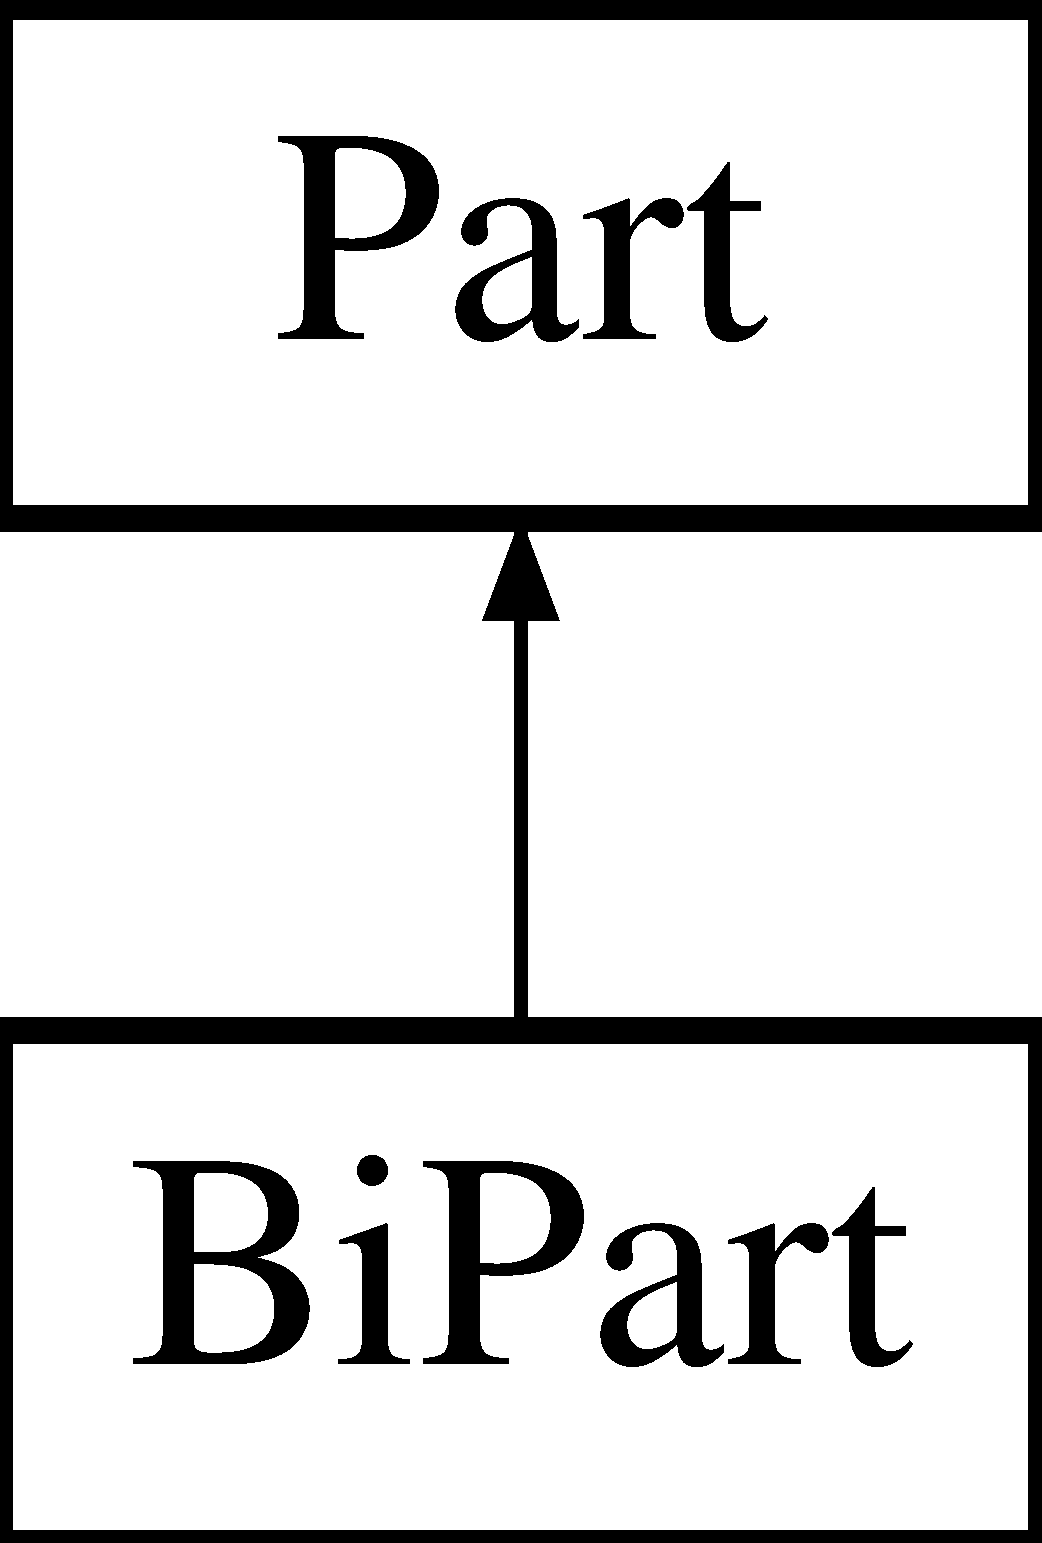
\includegraphics[height=2.000000cm]{classBiPart}
\end{center}
\end{figure}
\subsection*{Public Member Functions}
\begin{DoxyCompactItemize}
\item 
\hypertarget{classBiPart_aa3d9446a9207461c5b9ec328c3ef61ae}{{\bfseries Bi\-Part} (\hyperlink{classPart}{Part} $\ast$part1, \hyperlink{classPart}{Part} $\ast$part2, \hyperlink{classObjectiveValue}{Objective\-Value} $\ast$value=0)}\label{classBiPart_aa3d9446a9207461c5b9ec328c3ef61ae}

\item 
\hypertarget{classBiPart_ae80858643535d37f3cc96f0fccc947ff}{{\bfseries Bi\-Part} (\hyperlink{classBiPart}{Bi\-Part} $\ast$bi\-Part)}\label{classBiPart_ae80858643535d37f3cc96f0fccc947ff}

\item 
\hypertarget{classBiPart_a242f8d88da324a08bd296ea69cd7360f}{bool {\bfseries equal} (\hyperlink{classPart}{Part} $\ast$p)}\label{classBiPart_a242f8d88da324a08bd296ea69cd7360f}

\item 
\hypertarget{classBiPart_a2fb0a97551bcfc4a9bda5fa1307703d6}{void {\bfseries print} (bool endl=false)}\label{classBiPart_a2fb0a97551bcfc4a9bda5fa1307703d6}

\item 
\hypertarget{classBiPart_aace53eab6f4e8b2f676c0ed7d8f6c9b5}{int {\bfseries print\-Size} ()}\label{classBiPart_aace53eab6f4e8b2f676c0ed7d8f6c9b5}

\end{DoxyCompactItemize}
\subsection*{Public Attributes}
\begin{DoxyCompactItemize}
\item 
\hypertarget{classBiPart_a5846464cf88602318aa6c4f26976255b}{\hyperlink{classPart}{Part} $\ast$ {\bfseries first\-Part}}\label{classBiPart_a5846464cf88602318aa6c4f26976255b}

\item 
\hypertarget{classBiPart_a3497ede9e6226b6b71b39e481d07c63e}{\hyperlink{classPart}{Part} $\ast$ {\bfseries second\-Part}}\label{classBiPart_a3497ede9e6226b6b71b39e481d07c63e}

\end{DoxyCompactItemize}


\subsection{Detailed Description}
A bi-\/part is a subset of a bi-\/dimensional set of elements (individuals) 

The documentation for this class was generated from the following files\-:\begin{DoxyCompactItemize}
\item 
src/partition.\-hpp\item 
src/partition.\-cpp\end{DoxyCompactItemize}

\hypertarget{classBottleneckObjectiveValue}{\section{Bottleneck\-Objective\-Value Class Reference}
\label{classBottleneckObjectiveValue}\index{Bottleneck\-Objective\-Value@{Bottleneck\-Objective\-Value}}
}
Inheritance diagram for Bottleneck\-Objective\-Value\-:\begin{figure}[H]
\begin{center}
\leavevmode
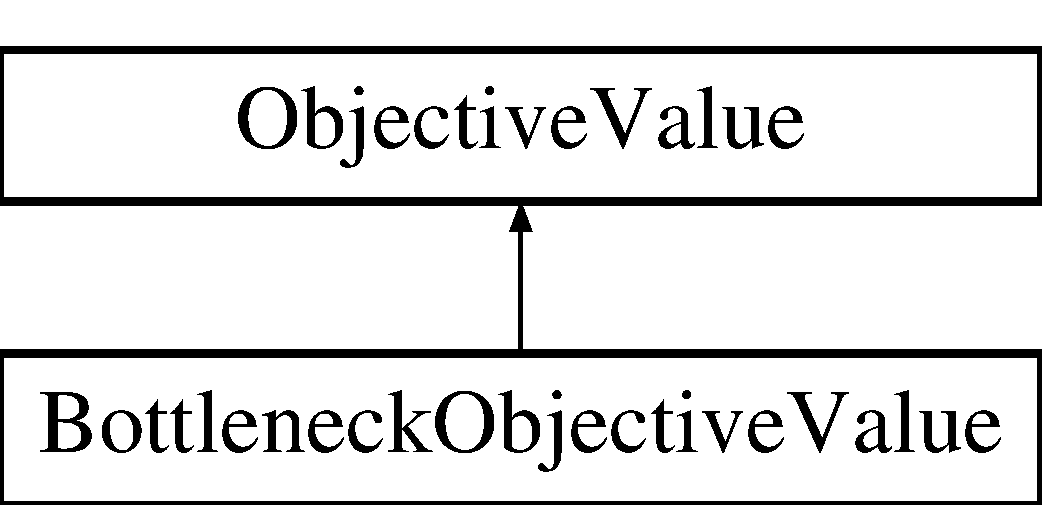
\includegraphics[height=2.000000cm]{classBottleneckObjectiveValue}
\end{center}
\end{figure}
\subsection*{Public Member Functions}
\begin{DoxyCompactItemize}
\item 
\hypertarget{classBottleneckObjectiveValue_a472c19dd35594975cdc8d63b06bec066}{{\bfseries Bottleneck\-Objective\-Value} (\hyperlink{classInformationBottleneck}{Information\-Bottleneck} $\ast$objective, int index=-\/1)}\label{classBottleneckObjectiveValue_a472c19dd35594975cdc8d63b06bec066}

\item 
\hypertarget{classBottleneckObjectiveValue_acca02ede3d42cbb71852339087bdff22}{void {\bfseries add} (\hyperlink{classObjectiveValue}{Objective\-Value} $\ast$value)}\label{classBottleneckObjectiveValue_acca02ede3d42cbb71852339087bdff22}

\item 
\hypertarget{classBottleneckObjectiveValue_a2a1bfd06ae2ae78f7e347703f1805984}{void {\bfseries compute} ()}\label{classBottleneckObjectiveValue_a2a1bfd06ae2ae78f7e347703f1805984}

\item 
\hypertarget{classBottleneckObjectiveValue_ac6672e91013a5667488e7fccbc452fed}{void {\bfseries compute} (\hyperlink{classObjectiveValue}{Objective\-Value} $\ast$value1, \hyperlink{classObjectiveValue}{Objective\-Value} $\ast$value2)}\label{classBottleneckObjectiveValue_ac6672e91013a5667488e7fccbc452fed}

\item 
\hypertarget{classBottleneckObjectiveValue_ae6edb61731a33a8c3c28c9de3f011fa9}{void {\bfseries compute} (Objective\-Value\-Set $\ast$value\-Set)}\label{classBottleneckObjectiveValue_ae6edb61731a33a8c3c28c9de3f011fa9}

\item 
\hypertarget{classBottleneckObjectiveValue_a20cd5a3dce433043a3ce9641fc6df8b3}{void {\bfseries normalize} (\hyperlink{classObjectiveValue}{Objective\-Value} $\ast$q)}\label{classBottleneckObjectiveValue_a20cd5a3dce433043a3ce9641fc6df8b3}

\item 
\hypertarget{classBottleneckObjectiveValue_a5dd538d1531ca10fc8b1261ee83be8f2}{void {\bfseries print} (bool verbose=true)}\label{classBottleneckObjectiveValue_a5dd538d1531ca10fc8b1261ee83be8f2}

\item 
\hypertarget{classBottleneckObjectiveValue_a76d0963588415208aca8da0d1f1b4600}{double {\bfseries get\-Value} (double param)}\label{classBottleneckObjectiveValue_a76d0963588415208aca8da0d1f1b4600}

\end{DoxyCompactItemize}
\subsection*{Public Attributes}
\begin{DoxyCompactItemize}
\item 
\hypertarget{classBottleneckObjectiveValue_a6229987020b8634ca238bb7d6d8904db}{int {\bfseries index}}\label{classBottleneckObjectiveValue_a6229987020b8634ca238bb7d6d8904db}

\item 
\hypertarget{classBottleneckObjectiveValue_a0e9546f57c845f33372ac3db29f8ea25}{double {\bfseries pk}}\label{classBottleneckObjectiveValue_a0e9546f57c845f33372ac3db29f8ea25}

\item 
\hypertarget{classBottleneckObjectiveValue_ac823f5e398f9ae9c75fe9151b29aac5b}{double $\ast$ {\bfseries pkj}}\label{classBottleneckObjectiveValue_ac823f5e398f9ae9c75fe9151b29aac5b}

\item 
\hypertarget{classBottleneckObjectiveValue_ac6c6fa26dac3f438159c5c7c6f1b4f3b}{double $\ast$ {\bfseries pj}}\label{classBottleneckObjectiveValue_ac6c6fa26dac3f438159c5c7c6f1b4f3b}

\item 
\hypertarget{classBottleneckObjectiveValue_a227ccad30a07de0b38e4678940b06338}{double {\bfseries Iki}}\label{classBottleneckObjectiveValue_a227ccad30a07de0b38e4678940b06338}

\item 
\hypertarget{classBottleneckObjectiveValue_a40c60ab77263afa0738968433d2d425f}{double {\bfseries Ikj}}\label{classBottleneckObjectiveValue_a40c60ab77263afa0738968433d2d425f}

\end{DoxyCompactItemize}


The documentation for this class was generated from the following files\-:\begin{DoxyCompactItemize}
\item 
src/information\-\_\-bottleneck.\-hpp\item 
src/information\-\_\-bottleneck.\-cpp\end{DoxyCompactItemize}

\hypertarget{classCompleteGraph}{\section{Complete\-Graph Class Reference}
\label{classCompleteGraph}\index{Complete\-Graph@{Complete\-Graph}}
}
Inheritance diagram for Complete\-Graph\-:\begin{figure}[H]
\begin{center}
\leavevmode
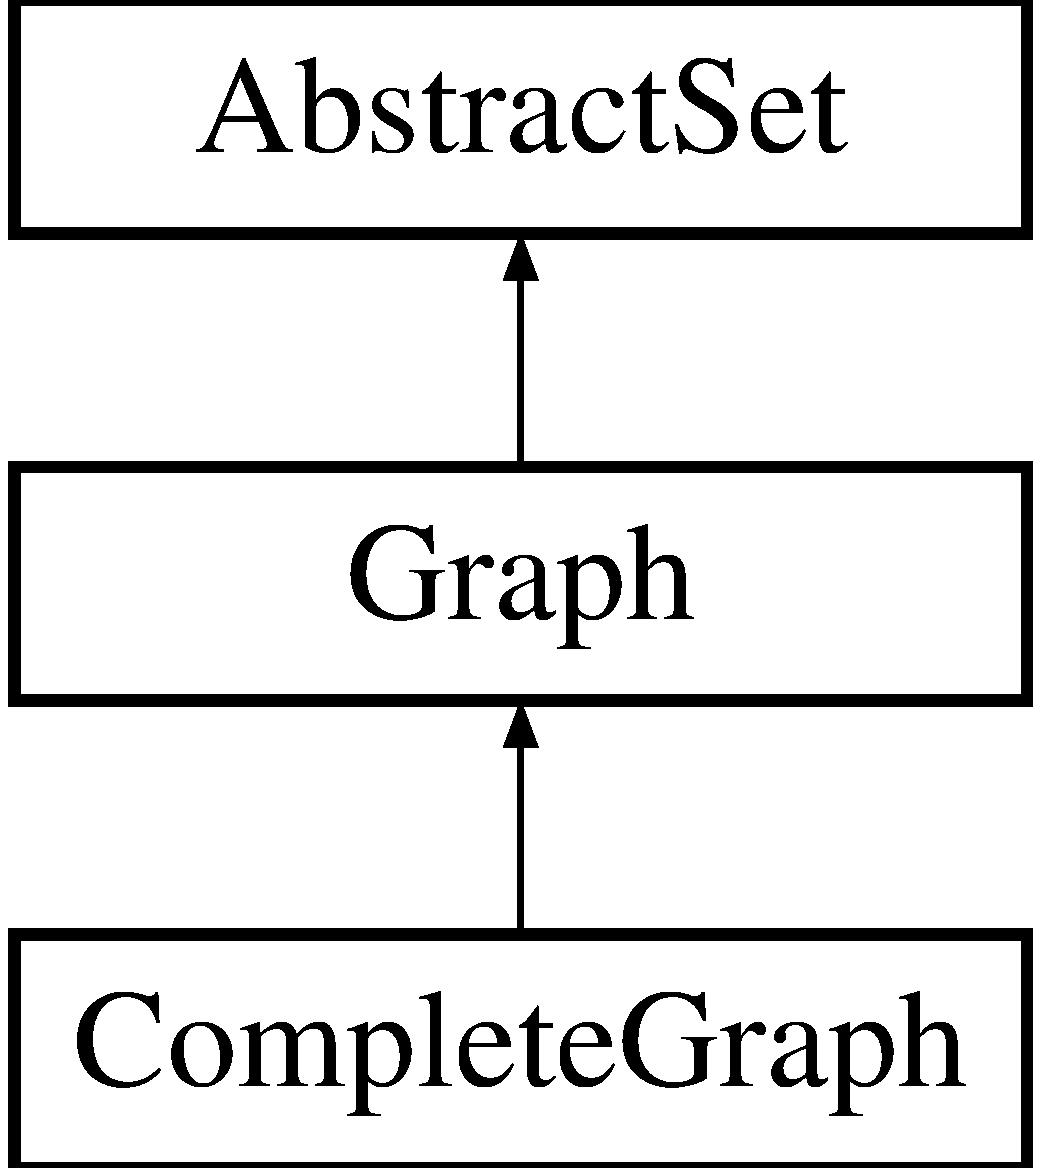
\includegraphics[height=3.000000cm]{classCompleteGraph}
\end{center}
\end{figure}
\subsection*{Public Member Functions}
\begin{DoxyCompactItemize}
\item 
\hypertarget{classCompleteGraph_ab74d38ce74de8bd6e413d416af89d9fa}{{\bfseries Complete\-Graph} (int v\-Num)}\label{classCompleteGraph_ab74d38ce74de8bd6e413d416af89d9fa}

\end{DoxyCompactItemize}
\subsection*{Additional Inherited Members}


The documentation for this class was generated from the following file\-:\begin{DoxyCompactItemize}
\item 
src/graph.\-hpp\end{DoxyCompactItemize}

\hypertarget{structDataPointStruct}{\section{Data\-Point\-Struct Struct Reference}
\label{structDataPointStruct}\index{Data\-Point\-Struct@{Data\-Point\-Struct}}
}
\subsection*{Public Attributes}
\begin{DoxyCompactItemize}
\item 
\hypertarget{structDataPointStruct_ab19cdad849d37de06c02cacc5ec50cce}{std\-::vector$<$ int $>$ {\bfseries parameters}}\label{structDataPointStruct_ab19cdad849d37de06c02cacc5ec50cce}

\item 
\hypertarget{structDataPointStruct_ae1dae54ff363ef8a6d946907b1621506}{float {\bfseries time}}\label{structDataPointStruct_ae1dae54ff363ef8a6d946907b1621506}

\item 
\hypertarget{structDataPointStruct_a6d345b8aa7e79cd06402446d73d19520}{int {\bfseries memory}}\label{structDataPointStruct_a6d345b8aa7e79cd06402446d73d19520}

\end{DoxyCompactItemize}


The documentation for this struct was generated from the following file\-:\begin{DoxyCompactItemize}
\item 
/home/lamarche/programming/optimal\-\_\-partition/src/timer.\-hpp\end{DoxyCompactItemize}

\hypertarget{classDataset}{\section{Dataset Class Reference}
\label{classDataset}\index{Dataset@{Dataset}}
}
\subsection*{Public Member Functions}
\begin{DoxyCompactItemize}
\item 
\hypertarget{classDataset_a8feaf2bb311910ab4d99d2e4bf1463b9}{void {\bfseries print} ()}\label{classDataset_a8feaf2bb311910ab4d99d2e4bf1463b9}

\item 
\hypertarget{classDataset_ac60d60df61e67a22b131642ab4dd06d4}{void {\bfseries build\-Dataset} ()}\label{classDataset_ac60d60df61e67a22b131642ab4dd06d4}

\item 
\hypertarget{classDataset_a9a50f1d277ee5fbd065e5e99ebe5b40b}{void {\bfseries init\-Values} (double v=0)}\label{classDataset_a9a50f1d277ee5fbd065e5e99ebe5b40b}

\item 
\hypertarget{classDataset_a6ac9666627e5f9d96660faff51b8bd8d}{void {\bfseries init\-Ref\-Values} (double v=0)}\label{classDataset_a6ac9666627e5f9d96660faff51b8bd8d}

\item 
\hypertarget{classDataset_a4b062bc0218c18b32e266d02b67ee8dd}{void {\bfseries add\-Label1} (std\-::string str)}\label{classDataset_a4b062bc0218c18b32e266d02b67ee8dd}

\item 
\hypertarget{classDataset_a7c4c161be1a352682d64a7a829366f4a}{void {\bfseries add\-Label2} (std\-::string str)}\label{classDataset_a7c4c161be1a352682d64a7a829366f4a}

\item 
\hypertarget{classDataset_a9a3da37b8e90e79207ee1e50ce22f953}{std\-::string {\bfseries get\-Label1} (int i)}\label{classDataset_a9a3da37b8e90e79207ee1e50ce22f953}

\item 
\hypertarget{classDataset_acf9e3bb76f7f220f2f4feeeff6841ac7}{std\-::string {\bfseries get\-Label2} (int j)}\label{classDataset_acf9e3bb76f7f220f2f4feeeff6841ac7}

\item 
\hypertarget{classDataset_abb1dc48765980e8559e9c3e358ca91cb}{int {\bfseries get\-Index1} (std\-::string s1)}\label{classDataset_abb1dc48765980e8559e9c3e358ca91cb}

\item 
\hypertarget{classDataset_a90c0f70c654055ae973c7167b565ec5d}{int {\bfseries get\-Index2} (std\-::string s2)}\label{classDataset_a90c0f70c654055ae973c7167b565ec5d}

\item 
\hypertarget{classDataset_a7c548cf3734e968d5b6b87ea91f3b57a}{double {\bfseries get\-Value} (int i, int j)}\label{classDataset_a7c548cf3734e968d5b6b87ea91f3b57a}

\item 
\hypertarget{classDataset_a9131823932772c581c556c3eeacc877c}{double {\bfseries get\-Ref\-Value} (int i, int j)}\label{classDataset_a9131823932772c581c556c3eeacc877c}

\item 
\hypertarget{classDataset_a0907b3685958a887937391cd9ae135ab}{double {\bfseries get\-Value} (std\-::string s1, std\-::string s2)}\label{classDataset_a0907b3685958a887937391cd9ae135ab}

\item 
\hypertarget{classDataset_a9235d598760d32cb9cfe32762489b07b}{double {\bfseries get\-Ref\-Value} (std\-::string s1, std\-::string s2)}\label{classDataset_a9235d598760d32cb9cfe32762489b07b}

\item 
\hypertarget{classDataset_a97ba235f117d9fd30fedfd4886e575c5}{void {\bfseries set\-Value} (int i, int j, double v)}\label{classDataset_a97ba235f117d9fd30fedfd4886e575c5}

\item 
\hypertarget{classDataset_ad13a7a7d14f3bf31b5e9c093c728a980}{void {\bfseries set\-Ref\-Value} (int i, int j, double v)}\label{classDataset_ad13a7a7d14f3bf31b5e9c093c728a980}

\item 
\hypertarget{classDataset_a09214d482be48183494020ef5c9466eb}{void {\bfseries set\-Value} (std\-::string s1, std\-::string s2, double v)}\label{classDataset_a09214d482be48183494020ef5c9466eb}

\item 
\hypertarget{classDataset_adf18516b4f2faae53ee90dce084d3bb1}{void {\bfseries set\-Ref\-Value} (std\-::string s1, std\-::string s2, double v)}\label{classDataset_adf18516b4f2faae53ee90dce084d3bb1}

\item 
\hypertarget{classDataset_af77b9e5bfbcc82307f811c06aa743372}{void {\bfseries increment\-Value} (int i, int j)}\label{classDataset_af77b9e5bfbcc82307f811c06aa743372}

\item 
\hypertarget{classDataset_a7326b8a0092ba1ebb44349c9eeb01440}{void {\bfseries increment\-Ref\-Value} (int i, int j)}\label{classDataset_a7326b8a0092ba1ebb44349c9eeb01440}

\item 
\hypertarget{classDataset_ab490e1dc5d017d6400a70f541f6c47ba}{void {\bfseries increment\-Value} (std\-::string s1, std\-::string s2)}\label{classDataset_ab490e1dc5d017d6400a70f541f6c47ba}

\item 
\hypertarget{classDataset_a5ec37adf418e434f06db698cd077f5b9}{void {\bfseries increment\-Ref\-Value} (std\-::string s1, std\-::string s2)}\label{classDataset_a5ec37adf418e434f06db698cd077f5b9}

\item 
\hypertarget{classDataset_a08bc430668dc243fde46b060745115b7}{double $\ast$ {\bfseries get\-Values1} (std\-::string s2)}\label{classDataset_a08bc430668dc243fde46b060745115b7}

\item 
\hypertarget{classDataset_af87c76f8b2f116d512af78e911e003cf}{double $\ast$ {\bfseries get\-Values2} (std\-::string s1)}\label{classDataset_af87c76f8b2f116d512af78e911e003cf}

\item 
\hypertarget{classDataset_a851bf5379def51280e64ea074f4334dd}{double $\ast$ {\bfseries get\-Ref\-Values1} (std\-::string s2)}\label{classDataset_a851bf5379def51280e64ea074f4334dd}

\item 
\hypertarget{classDataset_af70c89bf136f87b565495a2ac44dda69}{double $\ast$ {\bfseries get\-Ref\-Values2} (std\-::string s1)}\label{classDataset_af70c89bf136f87b565495a2ac44dda69}

\item 
\hypertarget{classDataset_aef2a876e783a9c7f802b63cb7a87aa9f}{double $\ast$ {\bfseries get\-Values} (bool order=true)}\label{classDataset_aef2a876e783a9c7f802b63cb7a87aa9f}

\item 
\hypertarget{classDataset_a4fe50eef91fe9730eb225859b8554512}{double $\ast$ {\bfseries get\-Ref\-Values} (bool order=true)}\label{classDataset_a4fe50eef91fe9730eb225859b8554512}

\end{DoxyCompactItemize}
\subsection*{Public Attributes}
\begin{DoxyCompactItemize}
\item 
\hypertarget{classDataset_a1cde47fee5ecc5f5f26c5ab3bb0331e3}{int {\bfseries size1}}\label{classDataset_a1cde47fee5ecc5f5f26c5ab3bb0331e3}

\item 
\hypertarget{classDataset_aaee19e6556e5168943fd128d38889a91}{int {\bfseries size2}}\label{classDataset_aaee19e6556e5168943fd128d38889a91}

\item 
\hypertarget{classDataset_ad7c03e01fa34e8986144340a6ddcf53c}{std\-::map$<$ std\-::string, int $>$ $\ast$ {\bfseries indices1}}\label{classDataset_ad7c03e01fa34e8986144340a6ddcf53c}

\item 
\hypertarget{classDataset_ade1e047d83395ee7f2241dbb25dd1455}{std\-::map$<$ std\-::string, int $>$ $\ast$ {\bfseries indices2}}\label{classDataset_ade1e047d83395ee7f2241dbb25dd1455}

\item 
\hypertarget{classDataset_a4598a42f6e129c3b073f62645a1c2893}{std\-::map$<$ int, std\-::string $>$ $\ast$ {\bfseries labels1}}\label{classDataset_a4598a42f6e129c3b073f62645a1c2893}

\item 
\hypertarget{classDataset_a01dc253aff164fb556d9d203b29a059f}{std\-::map$<$ int, std\-::string $>$ $\ast$ {\bfseries labels2}}\label{classDataset_a01dc253aff164fb556d9d203b29a059f}

\item 
\hypertarget{classDataset_a3554a3c5723716a89be372b946d04f54}{double $\ast$ {\bfseries values}}\label{classDataset_a3554a3c5723716a89be372b946d04f54}

\item 
\hypertarget{classDataset_a4a03dd925f63d0611c75223850c93569}{double $\ast$ {\bfseries ref\-Values}}\label{classDataset_a4a03dd925f63d0611c75223850c93569}

\end{DoxyCompactItemize}


The documentation for this class was generated from the following files\-:\begin{DoxyCompactItemize}
\item 
/home/lamarche/programming/optimal\-\_\-partition/src/dataset.\-hpp\item 
/home/lamarche/programming/optimal\-\_\-partition/src/dataset.\-cpp\end{DoxyCompactItemize}

\hypertarget{classDatatree}{\section{Datatree Class Reference}
\label{classDatatree}\index{Datatree@{Datatree}}
}
\subsection*{Public Member Functions}
\begin{DoxyCompactItemize}
\item 
\hypertarget{classDatatree_a8bb93df8a3fa33b71a264fb43ff6d964}{{\bfseries Datatree} (\hyperlink{classDatatree}{Datatree} \&tree)}\label{classDatatree_a8bb93df8a3fa33b71a264fb43ff6d964}

\item 
\hypertarget{classDatatree_a2b48ff5bfeca69cf5040ed34a9e994a5}{{\bfseries Datatree} (int vertex=-\/1)}\label{classDatatree_a2b48ff5bfeca69cf5040ed34a9e994a5}

\item 
\hypertarget{classDatatree_a0616b4cf3d6250609f58513ea93527b3}{void {\bfseries set\-Objective\-Function} (\hyperlink{classObjectiveFunction}{Objective\-Function} $\ast$objective)}\label{classDatatree_a0616b4cf3d6250609f58513ea93527b3}

\item 
\hypertarget{classDatatree_a3dc05fe23b3fab23ec5a0b23fdaf4fa8}{std\-::string {\bfseries to\-String} ()}\label{classDatatree_a3dc05fe23b3fab23ec5a0b23fdaf4fa8}

\item 
\hypertarget{classDatatree_a026a5e0a90635ef9a6333bfca2f24443}{Vertices $\ast$ {\bfseries get\-All\-Vertices} ()}\label{classDatatree_a026a5e0a90635ef9a6333bfca2f24443}

\item 
\hypertarget{classDatatree_a182d9d69820f49e271f98bd16799ff0a}{\hyperlink{classDatatree}{Datatree} $\ast$ {\bfseries add\-Child} (int v, bool print=true)}\label{classDatatree_a182d9d69820f49e271f98bd16799ff0a}

\item 
\hypertarget{classDatatree_ab022efbacb970f0cf6a96a872330c473}{\hyperlink{classDatatree}{Datatree} $\ast$ {\bfseries find\-Child} (int v)}\label{classDatatree_ab022efbacb970f0cf6a96a872330c473}

\item 
\hypertarget{classDatatree_a5109102d0c4e0585c3479be1d691da3c}{\hyperlink{classDatatree}{Datatree} $\ast$ {\bfseries find\-Or\-Add\-Child} (int v, bool print=true)}\label{classDatatree_a5109102d0c4e0585c3479be1d691da3c}

\item 
\hypertarget{classDatatree_a80edf7e5f07d5a06380d33d15d4c283e}{void {\bfseries add\-Bipartition} (\hyperlink{classDatatree}{Datatree} $\ast$n1, \hyperlink{classDatatree}{Datatree} $\ast$n2)}\label{classDatatree_a80edf7e5f07d5a06380d33d15d4c283e}

\item 
\hypertarget{classDatatree_a7ae2c6a5ca9d09767a6db92a2637ef56}{void {\bfseries compute\-Objective\-Values} ()}\label{classDatatree_a7ae2c6a5ca9d09767a6db92a2637ef56}

\item 
\hypertarget{classDatatree_a4cdd6b4b682af74478fc2b760816633b}{void {\bfseries normalize\-Objective\-Values} (\hyperlink{classObjectiveValue}{Objective\-Value} $\ast$max\-Objective\-Value=0)}\label{classDatatree_a4cdd6b4b682af74478fc2b760816633b}

\item 
\hypertarget{classDatatree_a7308791f14c13557f0d933c45e67cd8f}{void {\bfseries print\-Objective\-Values} ()}\label{classDatatree_a7308791f14c13557f0d933c45e67cd8f}

\item 
\hypertarget{classDatatree_a5e0d20a09169c369fd327e88101835dd}{void {\bfseries compute\-Optimal\-Partition} (double parameter)}\label{classDatatree_a5e0d20a09169c369fd327e88101835dd}

\item 
\hypertarget{classDatatree_a69d5034cf5a9d1a7af3d2213c93893cd}{void {\bfseries print\-Optimal\-Partition} (double parameter)}\label{classDatatree_a69d5034cf5a9d1a7af3d2213c93893cd}

\item 
\hypertarget{classDatatree_a0dcbcdce7d54262fff6cebb95783e557}{\hyperlink{classPartition}{Partition} $\ast$ {\bfseries get\-Optimal\-Partition} (double parameter)}\label{classDatatree_a0dcbcdce7d54262fff6cebb95783e557}

\item 
\hypertarget{classDatatree_a1a2db65768a7bccb3a2b526dc0cf5209}{void {\bfseries print} (bool verbose=false)}\label{classDatatree_a1a2db65768a7bccb3a2b526dc0cf5209}

\item 
\hypertarget{classDatatree_a351a7f2726c47274b0a227562f6b8978}{void {\bfseries print\-Vertices} (bool endl=true)}\label{classDatatree_a351a7f2726c47274b0a227562f6b8978}

\item 
\hypertarget{classDatatree_adfb6a2a5705f553b0ee94544849fe53c}{Part\-Set $\ast$ {\bfseries get\-Parts} ()}\label{classDatatree_adfb6a2a5705f553b0ee94544849fe53c}

\item 
\hypertarget{classDatatree_a3fb38bb2c99eaa53609eff28b1640ed4}{void {\bfseries print\-Parts} ()}\label{classDatatree_a3fb38bb2c99eaa53609eff28b1640ed4}

\item 
\hypertarget{classDatatree_a4e27d38736e49ceb96158a9e888a0a2e}{Partition\-List $\ast$ {\bfseries get\-All\-Partitions} ()}\label{classDatatree_a4e27d38736e49ceb96158a9e888a0a2e}

\item 
\hypertarget{classDatatree_a989234f1c876c6a27474d6340190e4b5}{int {\bfseries print\-Partitions} (bool print=true)}\label{classDatatree_a989234f1c876c6a27474d6340190e4b5}

\end{DoxyCompactItemize}
\subsection*{Public Attributes}
\begin{DoxyCompactItemize}
\item 
\hypertarget{classDatatree_aeff071fdfc96f70caebf7e309ff6ffc1}{int {\bfseries size}}\label{classDatatree_aeff071fdfc96f70caebf7e309ff6ffc1}

\item 
\hypertarget{classDatatree_a2a47058fa1c14a0f6fe039b58cec35eb}{int {\bfseries vertex}}\label{classDatatree_a2a47058fa1c14a0f6fe039b58cec35eb}

\item 
\hypertarget{classDatatree_ad119ac5d9567af4fa5c713dac7a80716}{bool {\bfseries whole\-Set}}\label{classDatatree_ad119ac5d9567af4fa5c713dac7a80716}

\item 
\hypertarget{classDatatree_a2fde0e1a8b36fda4b54ec2aabeb07412}{\hyperlink{classObjectiveFunction}{Objective\-Function} $\ast$ {\bfseries objective}}\label{classDatatree_a2fde0e1a8b36fda4b54ec2aabeb07412}

\item 
\hypertarget{classDatatree_ad07a0561536f6d6fbc04fdf0a564fa98}{\hyperlink{classDatatree}{Datatree} $\ast$ {\bfseries parent}}\label{classDatatree_ad07a0561536f6d6fbc04fdf0a564fa98}

\item 
\hypertarget{classDatatree_aa8e0282b874ca8ed141e483fd15040f0}{\hyperlink{classDatatree}{Datatree} $\ast$ {\bfseries complement}}\label{classDatatree_aa8e0282b874ca8ed141e483fd15040f0}

\item 
\hypertarget{classDatatree_af4cf6ba5a265fdfdd554bc8708d6508a}{Trees\-List $\ast$ {\bfseries complement\-List}}\label{classDatatree_af4cf6ba5a265fdfdd554bc8708d6508a}

\item 
\hypertarget{classDatatree_a5b3a31399892383f30b72a097cb05255}{Trees\-Set $\ast$ {\bfseries children}}\label{classDatatree_a5b3a31399892383f30b72a097cb05255}

\item 
\hypertarget{classDatatree_aae3f29ed73ad6981af6c179f1c753b5c}{\hyperlink{classObjectiveValue}{Objective\-Value} $\ast$ {\bfseries value}}\label{classDatatree_aae3f29ed73ad6981af6c179f1c753b5c}

\item 
\hypertarget{classDatatree_a1ee7d2704a67d56247a5a8dba84c57f1}{Bipartitions\-Set $\ast$ {\bfseries bipartitions}}\label{classDatatree_a1ee7d2704a67d56247a5a8dba84c57f1}

\item 
\hypertarget{classDatatree_ab05119987fb8d744edd73177a8afd4dc}{double {\bfseries optimal\-Value}}\label{classDatatree_ab05119987fb8d744edd73177a8afd4dc}

\item 
\hypertarget{classDatatree_af77422049ff1cd38f8bff3258df2f6f2}{Bipartition $\ast$ {\bfseries optimal\-Bipartition}}\label{classDatatree_af77422049ff1cd38f8bff3258df2f6f2}

\item 
\hypertarget{classDatatree_a6255f63e818a66b3b0e15c395bae06fb}{bool {\bfseries optimized}}\label{classDatatree_a6255f63e818a66b3b0e15c395bae06fb}

\end{DoxyCompactItemize}


The documentation for this class was generated from the following files\-:\begin{DoxyCompactItemize}
\item 
src/datatree.\-hpp\item 
src/datatree.\-cpp\end{DoxyCompactItemize}

\hypertarget{classFiliformGraph}{\section{Filiform\-Graph Class Reference}
\label{classFiliformGraph}\index{Filiform\-Graph@{Filiform\-Graph}}
}
Inheritance diagram for Filiform\-Graph\-:\begin{figure}[H]
\begin{center}
\leavevmode
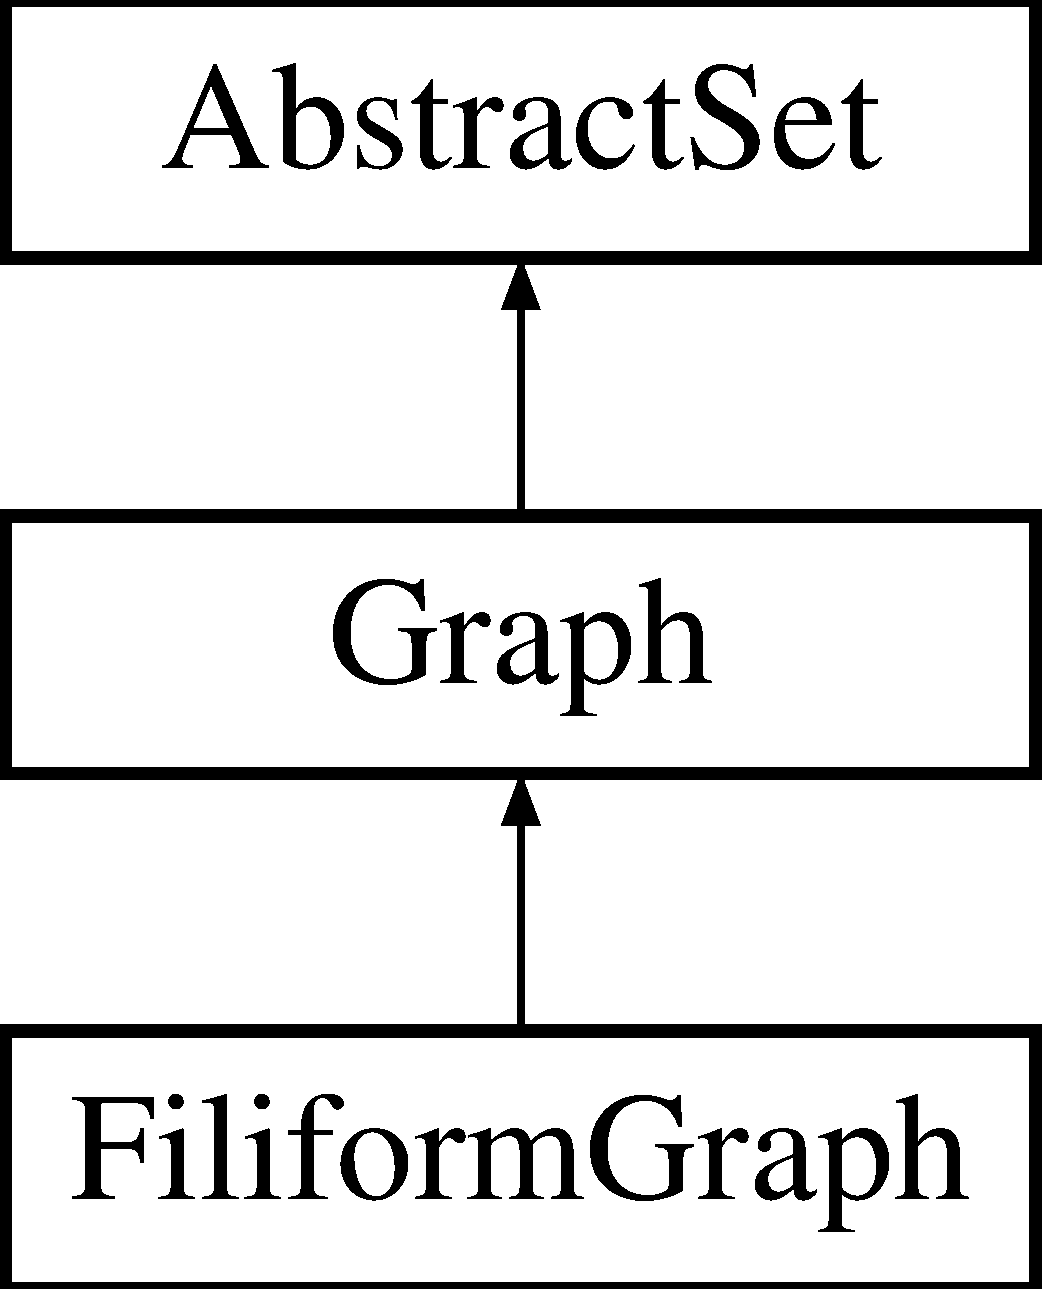
\includegraphics[height=3.000000cm]{classFiliformGraph}
\end{center}
\end{figure}
\subsection*{Public Member Functions}
\begin{DoxyCompactItemize}
\item 
\hypertarget{classFiliformGraph_a78e5ddfddf9f546254cb9430bb1aaccf}{{\bfseries Filiform\-Graph} (int v\-Num)}\label{classFiliformGraph_a78e5ddfddf9f546254cb9430bb1aaccf}

\end{DoxyCompactItemize}
\subsection*{Additional Inherited Members}


The documentation for this class was generated from the following files\-:\begin{DoxyCompactItemize}
\item 
src/graph.\-hpp\item 
src/graph.\-cpp\end{DoxyCompactItemize}

\hypertarget{classGraph}{\section{Graph Class Reference}
\label{classGraph}\index{Graph@{Graph}}
}
Inheritance diagram for Graph\-:\begin{figure}[H]
\begin{center}
\leavevmode
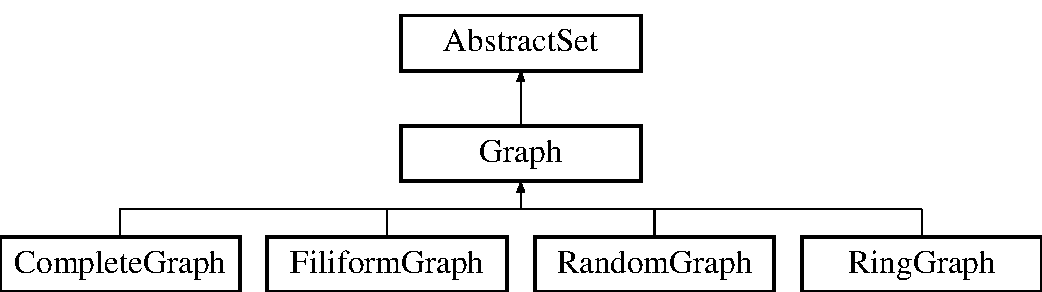
\includegraphics[height=3.000000cm]{classGraph}
\end{center}
\end{figure}
\subsection*{Public Member Functions}
\begin{DoxyCompactItemize}
\item 
\hypertarget{classGraph_a7e963f57fa2c368e79db1562112aed54}{{\bfseries Graph} (int size)}\label{classGraph_a7e963f57fa2c368e79db1562112aed54}

\item 
\hypertarget{classGraph_ae2f806a5d1fd576be15019f5386cc2e9}{void \hyperlink{classGraph_ae2f806a5d1fd576be15019f5386cc2e9}{set\-Random} ()}\label{classGraph_ae2f806a5d1fd576be15019f5386cc2e9}

\begin{DoxyCompactList}\small\item\em Randomly set the algebraic constraints for quick experiments (warning\-: this method is not always implemented) \end{DoxyCompactList}\item 
void \hyperlink{classGraph_a294aff8b11a1b11dae2b4cd39b78b91d}{set\-Objective\-Function} (\hyperlink{classObjectiveFunction}{Objective\-Function} $\ast$m)
\begin{DoxyCompactList}\small\item\em Set the objective that one wants to optimise. \end{DoxyCompactList}\item 
\hypertarget{classGraph_a2ecf3dd3c4897aa924da8e5c221a8509}{void \hyperlink{classGraph_a2ecf3dd3c4897aa924da8e5c221a8509}{print} ()}\label{classGraph_a2ecf3dd3c4897aa924da8e5c221a8509}

\begin{DoxyCompactList}\small\item\em Print the set and its algebraic constraints. \end{DoxyCompactList}\item 
\hypertarget{classGraph_a97b56f6ca766306c46778aab649acb93}{void {\bfseries add\-Edge} (int v1, int v2)}\label{classGraph_a97b56f6ca766306c46778aab649acb93}

\item 
\hypertarget{classGraph_aa68cd04b69f30175237dc951c14ed5ab}{void {\bfseries build\-From\-Binary} (int index)}\label{classGraph_aa68cd04b69f30175237dc951c14ed5ab}

\item 
\hypertarget{classGraph_a82a6e60e8156ce5920ab100301888df4}{bool {\bfseries are\-Adjacent} (int v1, int v2)}\label{classGraph_a82a6e60e8156ce5920ab100301888df4}

\item 
\hypertarget{classGraph_ac7e4433df9f5bf2daf9b656ca10a9447}{bool {\bfseries are\-Adjacent} (int v1, Vertices $\ast$v2)}\label{classGraph_ac7e4433df9f5bf2daf9b656ca10a9447}

\item 
\hypertarget{classGraph_a79fc06c760894df4a0672f8dd0cad813}{bool {\bfseries are\-Adjacent} (Vertices $\ast$v1, int v2)}\label{classGraph_a79fc06c760894df4a0672f8dd0cad813}

\item 
\hypertarget{classGraph_a9b9d58195496532784648a94d14a06ad}{bool {\bfseries are\-Adjacent} (Vertices $\ast$v1, Vertices $\ast$v2)}\label{classGraph_a9b9d58195496532784648a94d14a06ad}

\item 
\hypertarget{classGraph_a32d5402eb9ff745b679a2790142fae10}{bool {\bfseries are\-Adjacent} (int v1, V\-Vertices $\ast$v2)}\label{classGraph_a32d5402eb9ff745b679a2790142fae10}

\item 
\hypertarget{classGraph_ac4067cfdb2add845e54ace0dd90bac3c}{bool {\bfseries are\-Adjacent} (V\-Vertices $\ast$v1, int v2)}\label{classGraph_ac4067cfdb2add845e54ace0dd90bac3c}

\item 
\hypertarget{classGraph_a2e9ee0363fc146ad0681bdbaae99028b}{bool {\bfseries are\-Adjacent} (V\-Vertices $\ast$v1, V\-Vertices $\ast$v2)}\label{classGraph_a2e9ee0363fc146ad0681bdbaae99028b}

\item 
\hypertarget{classGraph_a44b45c4abab348e84369d0ebcbb2c120}{Vertices $\ast$ {\bfseries get\-Adjacent\-Vertices} (int v, int v\-Max=-\/1)}\label{classGraph_a44b45c4abab348e84369d0ebcbb2c120}

\item 
\hypertarget{classGraph_aee018750b2ee25ffee6f23a53d38d2bb}{void {\bfseries print\-Vertices} (Vertices $\ast$V)}\label{classGraph_aee018750b2ee25ffee6f23a53d38d2bb}

\item 
\hypertarget{classGraph_add6f4a13a70d1b15f370db0bd4669b90}{bool {\bfseries is\-Connected} ()}\label{classGraph_add6f4a13a70d1b15f370db0bd4669b90}

\item 
\hypertarget{classGraph_a269433faeb00d19be87c79569ecec4a0}{bool {\bfseries is\-Connected} (Vertices $\ast$V)}\label{classGraph_a269433faeb00d19be87c79569ecec4a0}

\item 
\hypertarget{classGraph_aea899acebf8ff5ed6ad466acb172e081}{void {\bfseries print\-Data\-Structure} (bool verbose=true)}\label{classGraph_aea899acebf8ff5ed6ad466acb172e081}

\item 
\hypertarget{classGraph_abfe064a8ae22d82ac4e3658c53ab6b4f}{Part\-Set $\ast$ {\bfseries get\-Parts} ()}\label{classGraph_abfe064a8ae22d82ac4e3658c53ab6b4f}

\item 
\hypertarget{classGraph_a96096076e108b089d6aad5f8552d81aa}{void {\bfseries print\-Parts} ()}\label{classGraph_a96096076e108b089d6aad5f8552d81aa}

\item 
\hypertarget{classGraph_a957d9c3a0bceddbec167d2eb63c3d447}{int {\bfseries print\-Partitions} (bool \hyperlink{classGraph_a2ecf3dd3c4897aa924da8e5c221a8509}{print}=true)}\label{classGraph_a957d9c3a0bceddbec167d2eb63c3d447}

\item 
\hypertarget{classGraph_a7714e4a70a69e7d78c2479f06970c453}{void \hyperlink{classGraph_a7714e4a70a69e7d78c2479f06970c453}{build\-Data\-Structure} ()}\label{classGraph_a7714e4a70a69e7d78c2479f06970c453}

\begin{DoxyCompactList}\small\item\em Build a proper data structure to represent the set and its algebraic constraints (warning\-: this method should always be called after instantiating and parameterising a set, and before calling any other method, such as \hyperlink{classGraph_a2ecf3dd3c4897aa924da8e5c221a8509}{print()}, \hyperlink{classGraph_a237d09042d6411b64075e7b62bb5afaf}{compute\-Objective\-Values()}, compute\-Optimal\-Partition (double parameter), etc.) \end{DoxyCompactList}\item 
\hypertarget{classGraph_a237d09042d6411b64075e7b62bb5afaf}{void \hyperlink{classGraph_a237d09042d6411b64075e7b62bb5afaf}{compute\-Objective\-Values} ()}\label{classGraph_a237d09042d6411b64075e7b62bb5afaf}

\begin{DoxyCompactList}\small\item\em Compute the value of the objective function for each feasible part (warning\-: set\-Objective\-Function (\hyperlink{classObjectiveFunction}{Objective\-Function} $\ast$objective) should have been called first) \end{DoxyCompactList}\item 
\hypertarget{classGraph_ad475ae837e3a0ba750ea9e7975ff1887}{void \hyperlink{classGraph_ad475ae837e3a0ba750ea9e7975ff1887}{normalize\-Objective\-Values} ()}\label{classGraph_ad475ae837e3a0ba750ea9e7975ff1887}

\begin{DoxyCompactList}\small\item\em Finish computing the value of the objective function for each feasible part when normalisation is required (warning\-: only after \hyperlink{classGraph_a237d09042d6411b64075e7b62bb5afaf}{compute\-Objective\-Values()} has been called) \end{DoxyCompactList}\item 
\hypertarget{classGraph_a353894a995807b625cf5713e79696a9d}{void \hyperlink{classGraph_a353894a995807b625cf5713e79696a9d}{print\-Objective\-Values} ()}\label{classGraph_a353894a995807b625cf5713e79696a9d}

\begin{DoxyCompactList}\small\item\em Print the value of the objective function for each feasible part. \end{DoxyCompactList}\item 
\hypertarget{classGraph_a78cfa04d5b7ea02297ec5014cd4e3356}{void {\bfseries build\-Data\-Structure\-With\-Slyce} ()}\label{classGraph_a78cfa04d5b7ea02297ec5014cd4e3356}

\item 
\hypertarget{classGraph_aa8e39f9a9010d0a010098b5090913550}{void {\bfseries slyce} (V\-Vertices $\ast$R, V\-Vertices $\ast$F, int m)}\label{classGraph_aa8e39f9a9010d0a010098b5090913550}

\item 
\hypertarget{classGraph_a518d7674ed8a64999503eb42834d4dcc}{void {\bfseries enumerate\-Subsets} (V\-Vertices $\ast$R, V\-Vertices $\ast$F, int m, int n, V\-Vertices $\ast$T, int q, int r)}\label{classGraph_a518d7674ed8a64999503eb42834d4dcc}

\item 
void \hyperlink{classGraph_a484517e8cda854dbaf158d7bdae19fe7}{compute\-Optimal\-Partition} (double parameter)
\begin{DoxyCompactList}\small\item\em Compute a partition that fits with the algebraic constraints and that optimises the objective function that has been specified. \end{DoxyCompactList}\item 
void \hyperlink{classGraph_a493dd2e19a08dd65ca49ac18944ad2cb}{print\-Optimal\-Partition} (double parameter)
\begin{DoxyCompactList}\small\item\em Compute and print a partition that fits with the algebraic constraints and that optimises the objective function that has been specified (warning\-: this method is not always implemented, but one can obtain a similar result by using get\-Optimal\-Partition (double parameter) and by calling \hyperlink{classGraph_a2ecf3dd3c4897aa924da8e5c221a8509}{print()} on the result) \end{DoxyCompactList}\item 
\hyperlink{classPartition}{Partition} $\ast$ \hyperlink{classGraph_a044d5401c498aa0c2d213986e7d747ca}{get\-Optimal\-Partition} (double parameter)
\begin{DoxyCompactList}\small\item\em Compute and return a partition that fits with the algebraic constraints and that optimises the objective function that has been specified (warning\-: this method is not always implemented, but one can obtain a similar result by using get\-Optimal\-Partition (double parameter) and by calling \hyperlink{classGraph_a2ecf3dd3c4897aa924da8e5c221a8509}{print()} on the result) \end{DoxyCompactList}\end{DoxyCompactItemize}
\subsection*{Public Attributes}
\begin{DoxyCompactItemize}
\item 
\hypertarget{classGraph_a726d5df1025e915e8785b6522331b21c}{int {\bfseries size}}\label{classGraph_a726d5df1025e915e8785b6522331b21c}

\item 
\hypertarget{classGraph_a081d860caac68d343992620e0331e8ac}{Vertices $\ast$$\ast$ {\bfseries adjacency\-Sets}}\label{classGraph_a081d860caac68d343992620e0331e8ac}

\item 
\hypertarget{classGraph_a63a6b3665080e19df5eb58f774f45db7}{\hyperlink{classGraphComponent}{Graph\-Component} $\ast$$\ast$ {\bfseries graph\-Components}}\label{classGraph_a63a6b3665080e19df5eb58f774f45db7}

\item 
\hypertarget{classGraph_aa013b53bc5d8a3c39e535005d749afa7}{Graph\-Component\-Set $\ast$ {\bfseries graph\-Component\-Set}}\label{classGraph_aa013b53bc5d8a3c39e535005d749afa7}

\item 
\hypertarget{classGraph_a8fb82bdd92337f7d7504f4f3a0ddcf8b}{bool $\ast$ {\bfseries reached\-Vertices}}\label{classGraph_a8fb82bdd92337f7d7504f4f3a0ddcf8b}

\item 
\hypertarget{classGraph_ab992346e14cdaba017ba3bdc0db162de}{\hyperlink{classObjectiveValue}{Objective\-Value} $\ast$ {\bfseries value}}\label{classGraph_ab992346e14cdaba017ba3bdc0db162de}

\end{DoxyCompactItemize}


\subsection{Member Function Documentation}
\hypertarget{classGraph_a484517e8cda854dbaf158d7bdae19fe7}{\index{Graph@{Graph}!compute\-Optimal\-Partition@{compute\-Optimal\-Partition}}
\index{compute\-Optimal\-Partition@{compute\-Optimal\-Partition}!Graph@{Graph}}
\subsubsection[{compute\-Optimal\-Partition}]{\setlength{\rightskip}{0pt plus 5cm}void Graph\-::compute\-Optimal\-Partition (
\begin{DoxyParamCaption}
\item[{double}]{parameter}
\end{DoxyParamCaption}
)\hspace{0.3cm}{\ttfamily [virtual]}}}\label{classGraph_a484517e8cda854dbaf158d7bdae19fe7}


Compute a partition that fits with the algebraic constraints and that optimises the objective function that has been specified. 


\begin{DoxyParams}{Parameters}
{\em parameter} & \-: The parameter of the objective function to be optimised (if the objective is parametrised) \\
\hline
\end{DoxyParams}


Implements \hyperlink{classAbstractSet_acfc3004f18192f38e32bb7a5a12ec8df}{Abstract\-Set}.

\hypertarget{classGraph_a044d5401c498aa0c2d213986e7d747ca}{\index{Graph@{Graph}!get\-Optimal\-Partition@{get\-Optimal\-Partition}}
\index{get\-Optimal\-Partition@{get\-Optimal\-Partition}!Graph@{Graph}}
\subsubsection[{get\-Optimal\-Partition}]{\setlength{\rightskip}{0pt plus 5cm}{\bf Partition} $\ast$ Graph\-::get\-Optimal\-Partition (
\begin{DoxyParamCaption}
\item[{double}]{parameter}
\end{DoxyParamCaption}
)\hspace{0.3cm}{\ttfamily [virtual]}}}\label{classGraph_a044d5401c498aa0c2d213986e7d747ca}


Compute and return a partition that fits with the algebraic constraints and that optimises the objective function that has been specified (warning\-: this method is not always implemented, but one can obtain a similar result by using get\-Optimal\-Partition (double parameter) and by calling \hyperlink{classGraph_a2ecf3dd3c4897aa924da8e5c221a8509}{print()} on the result) 


\begin{DoxyParams}{Parameters}
{\em parameter} & \-: The parameter of the objective function to be optimised (if the objective is parametrised) \\
\hline
\end{DoxyParams}
\begin{DoxyReturn}{Returns}
\-: The resulting optimal partition 
\end{DoxyReturn}


Implements \hyperlink{classAbstractSet_a48fd08c4b61ed46946bed6e19cd11194}{Abstract\-Set}.

\hypertarget{classGraph_a493dd2e19a08dd65ca49ac18944ad2cb}{\index{Graph@{Graph}!print\-Optimal\-Partition@{print\-Optimal\-Partition}}
\index{print\-Optimal\-Partition@{print\-Optimal\-Partition}!Graph@{Graph}}
\subsubsection[{print\-Optimal\-Partition}]{\setlength{\rightskip}{0pt plus 5cm}void Graph\-::print\-Optimal\-Partition (
\begin{DoxyParamCaption}
\item[{double}]{parameter}
\end{DoxyParamCaption}
)\hspace{0.3cm}{\ttfamily [virtual]}}}\label{classGraph_a493dd2e19a08dd65ca49ac18944ad2cb}


Compute and print a partition that fits with the algebraic constraints and that optimises the objective function that has been specified (warning\-: this method is not always implemented, but one can obtain a similar result by using get\-Optimal\-Partition (double parameter) and by calling \hyperlink{classGraph_a2ecf3dd3c4897aa924da8e5c221a8509}{print()} on the result) 


\begin{DoxyParams}{Parameters}
{\em parameter} & \-: The parameter of the objective function to be optimised (if the objective is parametrised) \\
\hline
\end{DoxyParams}


Implements \hyperlink{classAbstractSet_a82a9ce5c2d30690f0d1b83b034e92e1e}{Abstract\-Set}.

\hypertarget{classGraph_a294aff8b11a1b11dae2b4cd39b78b91d}{\index{Graph@{Graph}!set\-Objective\-Function@{set\-Objective\-Function}}
\index{set\-Objective\-Function@{set\-Objective\-Function}!Graph@{Graph}}
\subsubsection[{set\-Objective\-Function}]{\setlength{\rightskip}{0pt plus 5cm}void Graph\-::set\-Objective\-Function (
\begin{DoxyParamCaption}
\item[{{\bf Objective\-Function} $\ast$}]{objective}
\end{DoxyParamCaption}
)\hspace{0.3cm}{\ttfamily [virtual]}}}\label{classGraph_a294aff8b11a1b11dae2b4cd39b78b91d}


Set the objective that one wants to optimise. 


\begin{DoxyParams}{Parameters}
{\em objective} & \-: The objective function itself \\
\hline
\end{DoxyParams}


Implements \hyperlink{classAbstractSet_a7aef71679a18ab7965d1098da15b26c2}{Abstract\-Set}.



The documentation for this class was generated from the following files\-:\begin{DoxyCompactItemize}
\item 
/home/lamarche/programming/optimal\-\_\-partition/src/graph.\-hpp\item 
/home/lamarche/programming/optimal\-\_\-partition/src/graph.\-cpp\end{DoxyCompactItemize}

\hypertarget{classGraphComponent}{\section{Graph\-Component Class Reference}
\label{classGraphComponent}\index{Graph\-Component@{Graph\-Component}}
}
\subsection*{Public Member Functions}
\begin{DoxyCompactItemize}
\item 
\hypertarget{classGraphComponent_add1de7615139f01b7fbf155eb361e171}{{\bfseries Graph\-Component} (\hyperlink{classGraph}{Graph} $\ast$graph)}\label{classGraphComponent_add1de7615139f01b7fbf155eb361e171}

\item 
\hypertarget{classGraphComponent_a842a0bbe5e833bac1d1b43aefc685fa9}{void {\bfseries set\-Vertices} (std\-::list$<$ int $>$ $\ast$vertex\-List)}\label{classGraphComponent_a842a0bbe5e833bac1d1b43aefc685fa9}

\item 
\hypertarget{classGraphComponent_adaaf2cb4ac58af1995f1de5667b94e74}{void {\bfseries print\-Data\-Structure} (bool verbose=true)}\label{classGraphComponent_adaaf2cb4ac58af1995f1de5667b94e74}

\item 
\hypertarget{classGraphComponent_a467e8ea8da9b7b265daa3ceb5b624411}{void {\bfseries build\-Data\-Structure} ()}\label{classGraphComponent_a467e8ea8da9b7b265daa3ceb5b624411}

\item 
\hypertarget{classGraphComponent_a19e5e9cadd30dde9cf8309064016816a}{void {\bfseries compute\-Objective\-Values} ()}\label{classGraphComponent_a19e5e9cadd30dde9cf8309064016816a}

\item 
\hypertarget{classGraphComponent_aa206dc3321d1436bd8c957ee19a0952e}{void {\bfseries normalize\-Objective\-Values} ()}\label{classGraphComponent_aa206dc3321d1436bd8c957ee19a0952e}

\item 
\hypertarget{classGraphComponent_ade21156a32aab43d55d9bbbb07d3b9c5}{void {\bfseries print\-Objective\-Values} ()}\label{classGraphComponent_ade21156a32aab43d55d9bbbb07d3b9c5}

\item 
\hypertarget{classGraphComponent_a2d2b90ed866f4ae7173737558cdca0cd}{void {\bfseries compute\-Optimal\-Partition} (double parameter)}\label{classGraphComponent_a2d2b90ed866f4ae7173737558cdca0cd}

\item 
\hypertarget{classGraphComponent_af642a5a15cdbd4c07daea39fafdc9fb1}{void {\bfseries print\-Optimal\-Partition} (double parameter)}\label{classGraphComponent_af642a5a15cdbd4c07daea39fafdc9fb1}

\item 
\hypertarget{classGraphComponent_abed6e50213ba351bb2d0d155710e8be4}{\hyperlink{classPartition}{Partition} $\ast$ {\bfseries get\-Optimal\-Partition} (double parameter)}\label{classGraphComponent_abed6e50213ba351bb2d0d155710e8be4}

\end{DoxyCompactItemize}
\subsection*{Public Attributes}
\begin{DoxyCompactItemize}
\item 
\hypertarget{classGraphComponent_a3624962766b1475e0a93fdd47e7f736c}{int {\bfseries size}}\label{classGraphComponent_a3624962766b1475e0a93fdd47e7f736c}

\item 
\hypertarget{classGraphComponent_add037336c58d88b648e63f2532e2506b}{int $\ast$ {\bfseries vertices}}\label{classGraphComponent_add037336c58d88b648e63f2532e2506b}

\item 
\hypertarget{classGraphComponent_a4a3df3b388cb8fb288e74029ab7a0806}{std\-::map$<$ int, int $>$ $\ast$ {\bfseries order}}\label{classGraphComponent_a4a3df3b388cb8fb288e74029ab7a0806}

\item 
\hypertarget{classGraphComponent_ac12552650f43a1e2d13ddab6ce42ee75}{\hyperlink{classGraph}{Graph} $\ast$ {\bfseries graph}}\label{classGraphComponent_ac12552650f43a1e2d13ddab6ce42ee75}

\item 
\hypertarget{classGraphComponent_a53b6f7f9857c4cbf3232ec04d2b2d6ce}{\hyperlink{classDatatree}{Datatree} $\ast$ {\bfseries datatree}}\label{classGraphComponent_a53b6f7f9857c4cbf3232ec04d2b2d6ce}

\end{DoxyCompactItemize}


The documentation for this class was generated from the following files\-:\begin{DoxyCompactItemize}
\item 
/home/lamarche/programming/optimal\-\_\-partition/src/graph.\-hpp\item 
/home/lamarche/programming/optimal\-\_\-partition/src/graph.\-cpp\end{DoxyCompactItemize}

\hypertarget{classHHNode}{\section{H\-H\-Node Class Reference}
\label{classHHNode}\index{H\-H\-Node@{H\-H\-Node}}
}
\subsection*{Public Member Functions}
\begin{DoxyCompactItemize}
\item 
\hypertarget{classHHNode_aab9f99d78f7bc97c6cf532c29cd30b54}{{\bfseries H\-H\-Node} (\hyperlink{classHNode}{H\-Node} $\ast$node1, \hyperlink{classHNode}{H\-Node} $\ast$node2)}\label{classHHNode_aab9f99d78f7bc97c6cf532c29cd30b54}

\item 
\hypertarget{classHHNode_a3cbb049e2e5716418da87d63bd171401}{void {\bfseries add\-Child1} (\hyperlink{classHHNode}{H\-H\-Node} $\ast$node)}\label{classHHNode_a3cbb049e2e5716418da87d63bd171401}

\item 
\hypertarget{classHHNode_a42f070f81e0f971f784971cc1068fcf0}{void {\bfseries add\-Child2} (\hyperlink{classHHNode}{H\-H\-Node} $\ast$node)}\label{classHHNode_a42f070f81e0f971f784971cc1068fcf0}

\item 
\hypertarget{classHHNode_ae1dd902682e627f49924f14b6a79ce70}{void {\bfseries set\-Objective\-Function} (\hyperlink{classObjectiveFunction}{Objective\-Function} $\ast$m)}\label{classHHNode_ae1dd902682e627f49924f14b6a79ce70}

\item 
\hypertarget{classHHNode_a961a2374c8e59fa5ba1c804ec43c1eb3}{void {\bfseries print} ()}\label{classHHNode_a961a2374c8e59fa5ba1c804ec43c1eb3}

\item 
\hypertarget{classHHNode_af046ef2a00e95a03a04e77a5c2b4ec98}{void {\bfseries print\-Indices} (bool endl=false)}\label{classHHNode_af046ef2a00e95a03a04e77a5c2b4ec98}

\item 
\hypertarget{classHHNode_abcac0447fdc91214c7320442d82b8ef6}{void {\bfseries build\-Data\-Structure} ()}\label{classHHNode_abcac0447fdc91214c7320442d82b8ef6}

\item 
\hypertarget{classHHNode_aa352895af58b5bb268e2ed3f84cf1f50}{void {\bfseries compute\-Objective\-Values} ()}\label{classHHNode_aa352895af58b5bb268e2ed3f84cf1f50}

\item 
\hypertarget{classHHNode_ab633b4f761f69ccd90c008a3cd9e2af8}{void {\bfseries normalize\-Objective\-Values} (\hyperlink{classObjectiveValue}{Objective\-Value} $\ast$max\-Qual=0)}\label{classHHNode_ab633b4f761f69ccd90c008a3cd9e2af8}

\item 
\hypertarget{classHHNode_ae2fcb4d041f2fd8b36b8d7684fb6afce}{void {\bfseries print\-Objective\-Values} ()}\label{classHHNode_ae2fcb4d041f2fd8b36b8d7684fb6afce}

\item 
\hypertarget{classHHNode_ad5336d55619a2edf10c0eea7ad8d2554}{void {\bfseries compute\-Optimal\-Partition} (double parameter)}\label{classHHNode_ad5336d55619a2edf10c0eea7ad8d2554}

\item 
\hypertarget{classHHNode_a2c5e2be5a313b0e39aea2a21de3e4141}{void {\bfseries print\-Optimal\-Partition} (double parameter)}\label{classHHNode_a2c5e2be5a313b0e39aea2a21de3e4141}

\item 
\hypertarget{classHHNode_abbb1d78e16be3e35bad3631394a0b072}{void {\bfseries build\-Optimal\-Partition} (\hyperlink{classPartition}{Partition} $\ast$partition)}\label{classHHNode_abbb1d78e16be3e35bad3631394a0b072}

\end{DoxyCompactItemize}
\subsection*{Public Attributes}
\begin{DoxyCompactItemize}
\item 
\hypertarget{classHHNode_a8a4840e3b550450038aa6cf08664a10f}{\hyperlink{classHNode}{H\-Node} $\ast$ {\bfseries node1}}\label{classHHNode_a8a4840e3b550450038aa6cf08664a10f}

\item 
\hypertarget{classHHNode_a27dca34d04c73268088acaa3f63c3cf1}{\hyperlink{classHNode}{H\-Node} $\ast$ {\bfseries node2}}\label{classHHNode_a27dca34d04c73268088acaa3f63c3cf1}

\item 
\hypertarget{classHHNode_a30f76c1b6af3e718fed25daf3f201867}{H\-H\-Node\-Set $\ast$ {\bfseries children1}}\label{classHHNode_a30f76c1b6af3e718fed25daf3f201867}

\item 
\hypertarget{classHHNode_ae834d94db3d05c0611cae96b65310a3f}{H\-H\-Node\-Set $\ast$ {\bfseries children2}}\label{classHHNode_ae834d94db3d05c0611cae96b65310a3f}

\item 
\hypertarget{classHHNode_a699ca440cd845b1605ac39da167a3ef6}{\hyperlink{classObjectiveFunction}{Objective\-Function} $\ast$ {\bfseries objective}}\label{classHHNode_a699ca440cd845b1605ac39da167a3ef6}

\item 
\hypertarget{classHHNode_ae38edb82e59ed2a8265212861234bb86}{\hyperlink{classObjectiveValue}{Objective\-Value} $\ast$ {\bfseries value}}\label{classHHNode_ae38edb82e59ed2a8265212861234bb86}

\item 
\hypertarget{classHHNode_a95b0f06e417e1805649993b1105c0353}{double {\bfseries optimal\-Value}}\label{classHHNode_a95b0f06e417e1805649993b1105c0353}

\item 
\hypertarget{classHHNode_a4f9897665bc4098b16432f619cbb4545}{int {\bfseries optimal\-Cut}}\label{classHHNode_a4f9897665bc4098b16432f619cbb4545}

\end{DoxyCompactItemize}


The documentation for this class was generated from the following files\-:\begin{DoxyCompactItemize}
\item 
src/hierarchical\-\_\-hierarchical\-\_\-set.\-hpp\item 
src/hierarchical\-\_\-hierarchical\-\_\-set.\-cpp\end{DoxyCompactItemize}

\hypertarget{classHierarchicalHierarchicalSet}{\section{Hierarchical\-Hierarchical\-Set Class Reference}
\label{classHierarchicalHierarchicalSet}\index{Hierarchical\-Hierarchical\-Set@{Hierarchical\-Hierarchical\-Set}}
}
Inheritance diagram for Hierarchical\-Hierarchical\-Set\-:\begin{figure}[H]
\begin{center}
\leavevmode
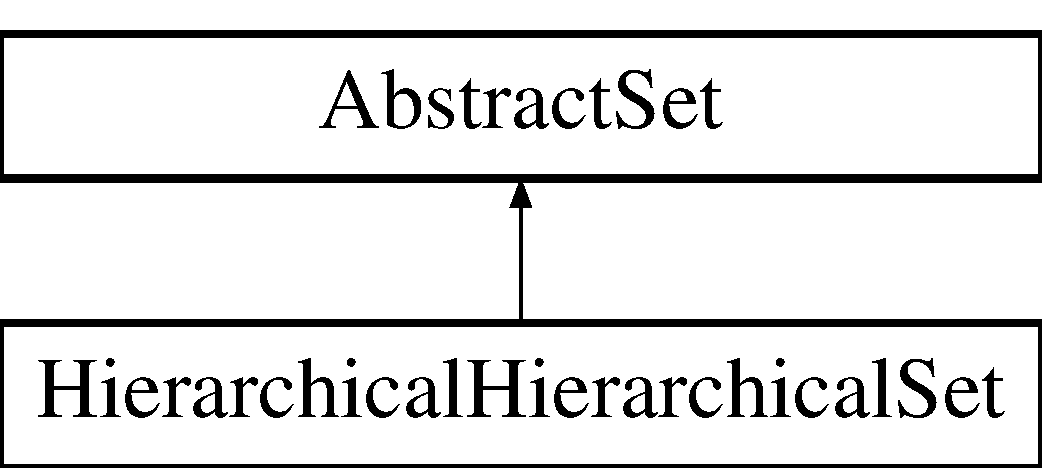
\includegraphics[height=2.000000cm]{classHierarchicalHierarchicalSet}
\end{center}
\end{figure}
\subsection*{Public Member Functions}
\begin{DoxyCompactItemize}
\item 
\hypertarget{classHierarchicalHierarchicalSet_ae239a8424b940258123c5d8505e44466}{{\bfseries Hierarchical\-Hierarchical\-Set} (\hyperlink{classHNode}{H\-Node} $\ast$hierarchy1, \hyperlink{classHNode}{H\-Node} $\ast$hierarchy2)}\label{classHierarchicalHierarchicalSet_ae239a8424b940258123c5d8505e44466}

\item 
\hypertarget{classHierarchicalHierarchicalSet_a668ee0e762ae12f0f059c35ccc6dc9fa}{void \hyperlink{classHierarchicalHierarchicalSet_a668ee0e762ae12f0f059c35ccc6dc9fa}{set\-Random} ()}\label{classHierarchicalHierarchicalSet_a668ee0e762ae12f0f059c35ccc6dc9fa}

\begin{DoxyCompactList}\small\item\em Randomly set the algebraic constraints for quick experiments (warning\-: this method is not always implemented) \end{DoxyCompactList}\item 
void \hyperlink{classHierarchicalHierarchicalSet_ae47e3171479131c47a2252b5c054ceef}{set\-Objective\-Function} (\hyperlink{classObjectiveFunction}{Objective\-Function} $\ast$m)
\begin{DoxyCompactList}\small\item\em Set the objective that one wants to optimise. \end{DoxyCompactList}\item 
\hypertarget{classHierarchicalHierarchicalSet_a860629468e7152d7642ef83f768673c2}{void \hyperlink{classHierarchicalHierarchicalSet_a860629468e7152d7642ef83f768673c2}{print} ()}\label{classHierarchicalHierarchicalSet_a860629468e7152d7642ef83f768673c2}

\begin{DoxyCompactList}\small\item\em Print the set and its algebraic constraints. \end{DoxyCompactList}\item 
\hypertarget{classHierarchicalHierarchicalSet_a28246c220b4d80d8c98cf8d6b5b46c01}{void \hyperlink{classHierarchicalHierarchicalSet_a28246c220b4d80d8c98cf8d6b5b46c01}{build\-Data\-Structure} ()}\label{classHierarchicalHierarchicalSet_a28246c220b4d80d8c98cf8d6b5b46c01}

\begin{DoxyCompactList}\small\item\em Build a proper data structure to represent the set and its algebraic constraints (warning\-: this method should always be called after instantiating and parameterising a set, and before calling any other method, such as \hyperlink{classHierarchicalHierarchicalSet_a860629468e7152d7642ef83f768673c2}{print()}, \hyperlink{classHierarchicalHierarchicalSet_a81ee649f6258596924766122c67264d0}{compute\-Objective\-Values()}, compute\-Optimal\-Partition (double parameter), etc.) \end{DoxyCompactList}\item 
\hypertarget{classHierarchicalHierarchicalSet_a81ee649f6258596924766122c67264d0}{void \hyperlink{classHierarchicalHierarchicalSet_a81ee649f6258596924766122c67264d0}{compute\-Objective\-Values} ()}\label{classHierarchicalHierarchicalSet_a81ee649f6258596924766122c67264d0}

\begin{DoxyCompactList}\small\item\em Compute the value of the objective function for each feasible part (warning\-: set\-Objective\-Function (\hyperlink{classObjectiveFunction}{Objective\-Function} $\ast$objective) should have been called first) \end{DoxyCompactList}\item 
\hypertarget{classHierarchicalHierarchicalSet_ad165d39a55c23f442f4e74ca8a44a670}{void \hyperlink{classHierarchicalHierarchicalSet_ad165d39a55c23f442f4e74ca8a44a670}{normalize\-Objective\-Values} ()}\label{classHierarchicalHierarchicalSet_ad165d39a55c23f442f4e74ca8a44a670}

\begin{DoxyCompactList}\small\item\em Finish computing the value of the objective function for each feasible part when normalisation is required (warning\-: only after \hyperlink{classHierarchicalHierarchicalSet_a81ee649f6258596924766122c67264d0}{compute\-Objective\-Values()} has been called) \end{DoxyCompactList}\item 
\hypertarget{classHierarchicalHierarchicalSet_a05460d7facce6998834eb3d5a738ae38}{void \hyperlink{classHierarchicalHierarchicalSet_a05460d7facce6998834eb3d5a738ae38}{print\-Objective\-Values} ()}\label{classHierarchicalHierarchicalSet_a05460d7facce6998834eb3d5a738ae38}

\begin{DoxyCompactList}\small\item\em Print the value of the objective function for each feasible part. \end{DoxyCompactList}\item 
void \hyperlink{classHierarchicalHierarchicalSet_a5fec3e288e01501f6ed0f56c7b64480c}{compute\-Optimal\-Partition} (double parameter)
\begin{DoxyCompactList}\small\item\em Compute a partition that fits with the algebraic constraints and that optimises the objective function that has been specified. \end{DoxyCompactList}\item 
void \hyperlink{classHierarchicalHierarchicalSet_a61add8eccdae0778ea3541b30b01b0b1}{print\-Optimal\-Partition} (double parameter)
\begin{DoxyCompactList}\small\item\em Compute and print a partition that fits with the algebraic constraints and that optimises the objective function that has been specified (warning\-: this method is not always implemented, but one can obtain a similar result by using get\-Optimal\-Partition (double parameter) and by calling \hyperlink{classHierarchicalHierarchicalSet_a860629468e7152d7642ef83f768673c2}{print()} on the result) \end{DoxyCompactList}\item 
\hyperlink{classPartition}{Partition} $\ast$ \hyperlink{classHierarchicalHierarchicalSet_ab7f3e53d68e2a0191d37cd3febdaa285}{get\-Optimal\-Partition} (double parameter)
\begin{DoxyCompactList}\small\item\em Compute and return a partition that fits with the algebraic constraints and that optimises the objective function that has been specified (warning\-: this method is not always implemented, but one can obtain a similar result by using get\-Optimal\-Partition (double parameter) and by calling \hyperlink{classHierarchicalHierarchicalSet_a860629468e7152d7642ef83f768673c2}{print()} on the result) \end{DoxyCompactList}\end{DoxyCompactItemize}
\subsection*{Public Attributes}
\begin{DoxyCompactItemize}
\item 
\hypertarget{classHierarchicalHierarchicalSet_aa193e677379c055b6a57d16327959761}{\hyperlink{classHNode}{H\-Node} $\ast$ {\bfseries hierarchy1}}\label{classHierarchicalHierarchicalSet_aa193e677379c055b6a57d16327959761}

\item 
\hypertarget{classHierarchicalHierarchicalSet_ae229ddda10755ffea2d84d57d95365da}{\hyperlink{classHNode}{H\-Node} $\ast$ {\bfseries hierarchy2}}\label{classHierarchicalHierarchicalSet_ae229ddda10755ffea2d84d57d95365da}

\item 
\hypertarget{classHierarchicalHierarchicalSet_a63cd4f47ffbeb8be1693cf6620961ac0}{\hyperlink{classHHNode}{H\-H\-Node} $\ast$ {\bfseries hyperarchy}}\label{classHierarchicalHierarchicalSet_a63cd4f47ffbeb8be1693cf6620961ac0}

\end{DoxyCompactItemize}


\subsection{Member Function Documentation}
\hypertarget{classHierarchicalHierarchicalSet_a5fec3e288e01501f6ed0f56c7b64480c}{\index{Hierarchical\-Hierarchical\-Set@{Hierarchical\-Hierarchical\-Set}!compute\-Optimal\-Partition@{compute\-Optimal\-Partition}}
\index{compute\-Optimal\-Partition@{compute\-Optimal\-Partition}!HierarchicalHierarchicalSet@{Hierarchical\-Hierarchical\-Set}}
\subsubsection[{compute\-Optimal\-Partition}]{\setlength{\rightskip}{0pt plus 5cm}void Hierarchical\-Hierarchical\-Set\-::compute\-Optimal\-Partition (
\begin{DoxyParamCaption}
\item[{double}]{parameter}
\end{DoxyParamCaption}
)\hspace{0.3cm}{\ttfamily [virtual]}}}\label{classHierarchicalHierarchicalSet_a5fec3e288e01501f6ed0f56c7b64480c}


Compute a partition that fits with the algebraic constraints and that optimises the objective function that has been specified. 


\begin{DoxyParams}{Parameters}
{\em parameter} & \-: The parameter of the objective function to be optimised (if the objective is parametrised) \\
\hline
\end{DoxyParams}


Implements \hyperlink{classAbstractSet_acfc3004f18192f38e32bb7a5a12ec8df}{Abstract\-Set}.

\hypertarget{classHierarchicalHierarchicalSet_ab7f3e53d68e2a0191d37cd3febdaa285}{\index{Hierarchical\-Hierarchical\-Set@{Hierarchical\-Hierarchical\-Set}!get\-Optimal\-Partition@{get\-Optimal\-Partition}}
\index{get\-Optimal\-Partition@{get\-Optimal\-Partition}!HierarchicalHierarchicalSet@{Hierarchical\-Hierarchical\-Set}}
\subsubsection[{get\-Optimal\-Partition}]{\setlength{\rightskip}{0pt plus 5cm}{\bf Partition} $\ast$ Hierarchical\-Hierarchical\-Set\-::get\-Optimal\-Partition (
\begin{DoxyParamCaption}
\item[{double}]{parameter}
\end{DoxyParamCaption}
)\hspace{0.3cm}{\ttfamily [virtual]}}}\label{classHierarchicalHierarchicalSet_ab7f3e53d68e2a0191d37cd3febdaa285}


Compute and return a partition that fits with the algebraic constraints and that optimises the objective function that has been specified (warning\-: this method is not always implemented, but one can obtain a similar result by using get\-Optimal\-Partition (double parameter) and by calling \hyperlink{classHierarchicalHierarchicalSet_a860629468e7152d7642ef83f768673c2}{print()} on the result) 


\begin{DoxyParams}{Parameters}
{\em parameter} & \-: The parameter of the objective function to be optimised (if the objective is parametrised) \\
\hline
\end{DoxyParams}
\begin{DoxyReturn}{Returns}
\-: The resulting optimal partition 
\end{DoxyReturn}


Implements \hyperlink{classAbstractSet_a48fd08c4b61ed46946bed6e19cd11194}{Abstract\-Set}.

\hypertarget{classHierarchicalHierarchicalSet_a61add8eccdae0778ea3541b30b01b0b1}{\index{Hierarchical\-Hierarchical\-Set@{Hierarchical\-Hierarchical\-Set}!print\-Optimal\-Partition@{print\-Optimal\-Partition}}
\index{print\-Optimal\-Partition@{print\-Optimal\-Partition}!HierarchicalHierarchicalSet@{Hierarchical\-Hierarchical\-Set}}
\subsubsection[{print\-Optimal\-Partition}]{\setlength{\rightskip}{0pt plus 5cm}void Hierarchical\-Hierarchical\-Set\-::print\-Optimal\-Partition (
\begin{DoxyParamCaption}
\item[{double}]{parameter}
\end{DoxyParamCaption}
)\hspace{0.3cm}{\ttfamily [virtual]}}}\label{classHierarchicalHierarchicalSet_a61add8eccdae0778ea3541b30b01b0b1}


Compute and print a partition that fits with the algebraic constraints and that optimises the objective function that has been specified (warning\-: this method is not always implemented, but one can obtain a similar result by using get\-Optimal\-Partition (double parameter) and by calling \hyperlink{classHierarchicalHierarchicalSet_a860629468e7152d7642ef83f768673c2}{print()} on the result) 


\begin{DoxyParams}{Parameters}
{\em parameter} & \-: The parameter of the objective function to be optimised (if the objective is parametrised) \\
\hline
\end{DoxyParams}


Implements \hyperlink{classAbstractSet_a82a9ce5c2d30690f0d1b83b034e92e1e}{Abstract\-Set}.

\hypertarget{classHierarchicalHierarchicalSet_ae47e3171479131c47a2252b5c054ceef}{\index{Hierarchical\-Hierarchical\-Set@{Hierarchical\-Hierarchical\-Set}!set\-Objective\-Function@{set\-Objective\-Function}}
\index{set\-Objective\-Function@{set\-Objective\-Function}!HierarchicalHierarchicalSet@{Hierarchical\-Hierarchical\-Set}}
\subsubsection[{set\-Objective\-Function}]{\setlength{\rightskip}{0pt plus 5cm}void Hierarchical\-Hierarchical\-Set\-::set\-Objective\-Function (
\begin{DoxyParamCaption}
\item[{{\bf Objective\-Function} $\ast$}]{objective}
\end{DoxyParamCaption}
)\hspace{0.3cm}{\ttfamily [virtual]}}}\label{classHierarchicalHierarchicalSet_ae47e3171479131c47a2252b5c054ceef}


Set the objective that one wants to optimise. 


\begin{DoxyParams}{Parameters}
{\em objective} & \-: The objective function itself \\
\hline
\end{DoxyParams}


Implements \hyperlink{classAbstractSet_a7aef71679a18ab7965d1098da15b26c2}{Abstract\-Set}.



The documentation for this class was generated from the following files\-:\begin{DoxyCompactItemize}
\item 
src/hierarchical\-\_\-hierarchical\-\_\-set.\-hpp\item 
src/hierarchical\-\_\-hierarchical\-\_\-set.\-cpp\end{DoxyCompactItemize}

\hypertarget{classHierarchicalOrderedSet}{\section{Hierarchical\-Ordered\-Set Class Reference}
\label{classHierarchicalOrderedSet}\index{Hierarchical\-Ordered\-Set@{Hierarchical\-Ordered\-Set}}
}
Inheritance diagram for Hierarchical\-Ordered\-Set\-:\begin{figure}[H]
\begin{center}
\leavevmode
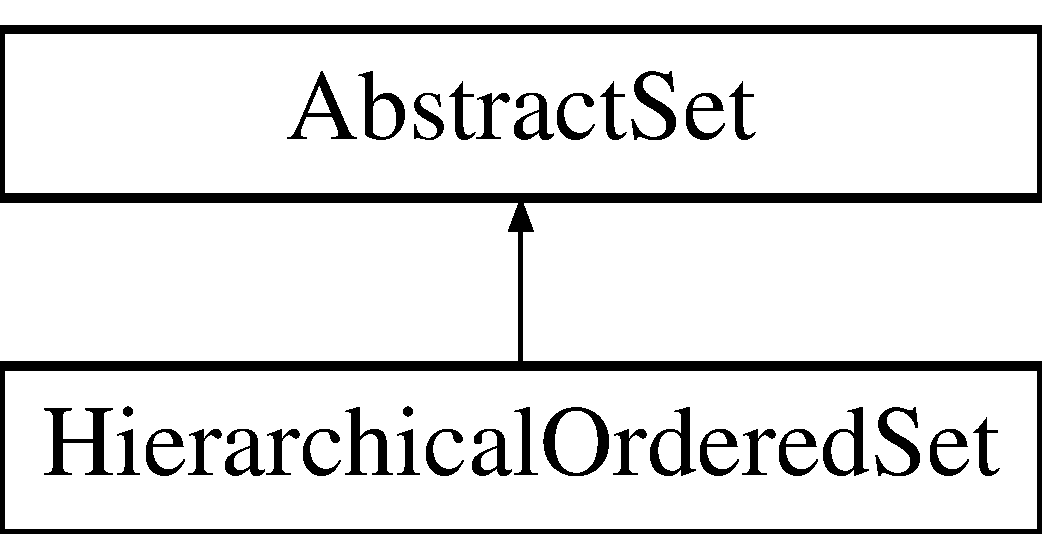
\includegraphics[height=2.000000cm]{classHierarchicalOrderedSet}
\end{center}
\end{figure}
\subsection*{Public Member Functions}
\begin{DoxyCompactItemize}
\item 
\hypertarget{classHierarchicalOrderedSet_a0cba386ea748272d65cad23b0f6ed585}{{\bfseries Hierarchical\-Ordered\-Set} (\hyperlink{classHONode}{H\-O\-Node} $\ast$hierarchy, int size)}\label{classHierarchicalOrderedSet_a0cba386ea748272d65cad23b0f6ed585}

\item 
\hypertarget{classHierarchicalOrderedSet_a7e1c018e4e9608dee3519480f3929146}{void \hyperlink{classHierarchicalOrderedSet_a7e1c018e4e9608dee3519480f3929146}{set\-Random} ()}\label{classHierarchicalOrderedSet_a7e1c018e4e9608dee3519480f3929146}

\begin{DoxyCompactList}\small\item\em Randomly set the algebraic constraints for quick experiments (warning\-: this method is not always implemented) \end{DoxyCompactList}\item 
void \hyperlink{classHierarchicalOrderedSet_a813f90e2aff889461b9e089b7ff460bc}{set\-Objective\-Function} (\hyperlink{classObjectiveFunction}{Objective\-Function} $\ast$m)
\begin{DoxyCompactList}\small\item\em Set the objective that one wants to optimise. \end{DoxyCompactList}\item 
\hypertarget{classHierarchicalOrderedSet_adabb092a33f0a552d4a0e0a8cd8221bb}{void \hyperlink{classHierarchicalOrderedSet_adabb092a33f0a552d4a0e0a8cd8221bb}{print} ()}\label{classHierarchicalOrderedSet_adabb092a33f0a552d4a0e0a8cd8221bb}

\begin{DoxyCompactList}\small\item\em Print the set and its algebraic constraints. \end{DoxyCompactList}\item 
\hypertarget{classHierarchicalOrderedSet_a9672b017eee7d3b43d00e66db85f49b6}{void \hyperlink{classHierarchicalOrderedSet_a9672b017eee7d3b43d00e66db85f49b6}{build\-Data\-Structure} ()}\label{classHierarchicalOrderedSet_a9672b017eee7d3b43d00e66db85f49b6}

\begin{DoxyCompactList}\small\item\em Build a proper data structure to represent the set and its algebraic constraints (warning\-: this method should always be called after instantiating and parameterising a set, and before calling any other method, such as \hyperlink{classHierarchicalOrderedSet_adabb092a33f0a552d4a0e0a8cd8221bb}{print()}, \hyperlink{classHierarchicalOrderedSet_aa1dc2e3a630f4bb3633fa008c9764ef4}{compute\-Objective\-Values()}, compute\-Optimal\-Partition (double parameter), etc.) \end{DoxyCompactList}\item 
\hypertarget{classHierarchicalOrderedSet_aa1dc2e3a630f4bb3633fa008c9764ef4}{void \hyperlink{classHierarchicalOrderedSet_aa1dc2e3a630f4bb3633fa008c9764ef4}{compute\-Objective\-Values} ()}\label{classHierarchicalOrderedSet_aa1dc2e3a630f4bb3633fa008c9764ef4}

\begin{DoxyCompactList}\small\item\em Compute the value of the objective function for each feasible part (warning\-: set\-Objective\-Function (\hyperlink{classObjectiveFunction}{Objective\-Function} $\ast$objective) should have been called first) \end{DoxyCompactList}\item 
\hypertarget{classHierarchicalOrderedSet_a7ee23f9f75bd6351c47751898ea02c18}{void \hyperlink{classHierarchicalOrderedSet_a7ee23f9f75bd6351c47751898ea02c18}{normalize\-Objective\-Values} ()}\label{classHierarchicalOrderedSet_a7ee23f9f75bd6351c47751898ea02c18}

\begin{DoxyCompactList}\small\item\em Finish computing the value of the objective function for each feasible part when normalisation is required (warning\-: only after \hyperlink{classHierarchicalOrderedSet_aa1dc2e3a630f4bb3633fa008c9764ef4}{compute\-Objective\-Values()} has been called) \end{DoxyCompactList}\item 
\hypertarget{classHierarchicalOrderedSet_a08d92f646e5caa37d431cc212ac73267}{void \hyperlink{classHierarchicalOrderedSet_a08d92f646e5caa37d431cc212ac73267}{print\-Objective\-Values} ()}\label{classHierarchicalOrderedSet_a08d92f646e5caa37d431cc212ac73267}

\begin{DoxyCompactList}\small\item\em Print the value of the objective function for each feasible part. \end{DoxyCompactList}\item 
void \hyperlink{classHierarchicalOrderedSet_aaaf67ab7d39ab2ca599c0c5a6ac22ce6}{compute\-Optimal\-Partition} (double parameter)
\begin{DoxyCompactList}\small\item\em Compute a partition that fits with the algebraic constraints and that optimises the objective function that has been specified. \end{DoxyCompactList}\item 
void \hyperlink{classHierarchicalOrderedSet_ae4df851956e9f11dce35c726b01c2bad}{print\-Optimal\-Partition} (double parameter)
\begin{DoxyCompactList}\small\item\em Compute and print a partition that fits with the algebraic constraints and that optimises the objective function that has been specified (warning\-: this method is not always implemented, but one can obtain a similar result by using get\-Optimal\-Partition (double parameter) and by calling \hyperlink{classHierarchicalOrderedSet_adabb092a33f0a552d4a0e0a8cd8221bb}{print()} on the result) \end{DoxyCompactList}\item 
\hyperlink{classPartition}{Partition} $\ast$ \hyperlink{classHierarchicalOrderedSet_a627ce416d730e03c9d807366e4a79a78}{get\-Optimal\-Partition} (double parameter)
\begin{DoxyCompactList}\small\item\em Compute and return a partition that fits with the algebraic constraints and that optimises the objective function that has been specified (warning\-: this method is not always implemented, but one can obtain a similar result by using get\-Optimal\-Partition (double parameter) and by calling \hyperlink{classHierarchicalOrderedSet_adabb092a33f0a552d4a0e0a8cd8221bb}{print()} on the result) \end{DoxyCompactList}\end{DoxyCompactItemize}
\subsection*{Public Attributes}
\begin{DoxyCompactItemize}
\item 
\hypertarget{classHierarchicalOrderedSet_af9556ecd472342223afb1e215a263302}{int {\bfseries size}}\label{classHierarchicalOrderedSet_af9556ecd472342223afb1e215a263302}

\item 
\hypertarget{classHierarchicalOrderedSet_af0ca5b9cceec4d1552eeea4bf276ae31}{\hyperlink{classHONode}{H\-O\-Node} $\ast$ {\bfseries hierarchy}}\label{classHierarchicalOrderedSet_af0ca5b9cceec4d1552eeea4bf276ae31}

\end{DoxyCompactItemize}


\subsection{Member Function Documentation}
\hypertarget{classHierarchicalOrderedSet_aaaf67ab7d39ab2ca599c0c5a6ac22ce6}{\index{Hierarchical\-Ordered\-Set@{Hierarchical\-Ordered\-Set}!compute\-Optimal\-Partition@{compute\-Optimal\-Partition}}
\index{compute\-Optimal\-Partition@{compute\-Optimal\-Partition}!HierarchicalOrderedSet@{Hierarchical\-Ordered\-Set}}
\subsubsection[{compute\-Optimal\-Partition}]{\setlength{\rightskip}{0pt plus 5cm}void Hierarchical\-Ordered\-Set\-::compute\-Optimal\-Partition (
\begin{DoxyParamCaption}
\item[{double}]{parameter}
\end{DoxyParamCaption}
)\hspace{0.3cm}{\ttfamily [virtual]}}}\label{classHierarchicalOrderedSet_aaaf67ab7d39ab2ca599c0c5a6ac22ce6}


Compute a partition that fits with the algebraic constraints and that optimises the objective function that has been specified. 


\begin{DoxyParams}{Parameters}
{\em parameter} & \-: The parameter of the objective function to be optimised (if the objective is parametrised) \\
\hline
\end{DoxyParams}


Implements \hyperlink{classAbstractSet_acfc3004f18192f38e32bb7a5a12ec8df}{Abstract\-Set}.

\hypertarget{classHierarchicalOrderedSet_a627ce416d730e03c9d807366e4a79a78}{\index{Hierarchical\-Ordered\-Set@{Hierarchical\-Ordered\-Set}!get\-Optimal\-Partition@{get\-Optimal\-Partition}}
\index{get\-Optimal\-Partition@{get\-Optimal\-Partition}!HierarchicalOrderedSet@{Hierarchical\-Ordered\-Set}}
\subsubsection[{get\-Optimal\-Partition}]{\setlength{\rightskip}{0pt plus 5cm}{\bf Partition} $\ast$ Hierarchical\-Ordered\-Set\-::get\-Optimal\-Partition (
\begin{DoxyParamCaption}
\item[{double}]{parameter}
\end{DoxyParamCaption}
)\hspace{0.3cm}{\ttfamily [virtual]}}}\label{classHierarchicalOrderedSet_a627ce416d730e03c9d807366e4a79a78}


Compute and return a partition that fits with the algebraic constraints and that optimises the objective function that has been specified (warning\-: this method is not always implemented, but one can obtain a similar result by using get\-Optimal\-Partition (double parameter) and by calling \hyperlink{classHierarchicalOrderedSet_adabb092a33f0a552d4a0e0a8cd8221bb}{print()} on the result) 


\begin{DoxyParams}{Parameters}
{\em parameter} & \-: The parameter of the objective function to be optimised (if the objective is parametrised) \\
\hline
\end{DoxyParams}
\begin{DoxyReturn}{Returns}
\-: The resulting optimal partition 
\end{DoxyReturn}


Implements \hyperlink{classAbstractSet_a48fd08c4b61ed46946bed6e19cd11194}{Abstract\-Set}.

\hypertarget{classHierarchicalOrderedSet_ae4df851956e9f11dce35c726b01c2bad}{\index{Hierarchical\-Ordered\-Set@{Hierarchical\-Ordered\-Set}!print\-Optimal\-Partition@{print\-Optimal\-Partition}}
\index{print\-Optimal\-Partition@{print\-Optimal\-Partition}!HierarchicalOrderedSet@{Hierarchical\-Ordered\-Set}}
\subsubsection[{print\-Optimal\-Partition}]{\setlength{\rightskip}{0pt plus 5cm}void Hierarchical\-Ordered\-Set\-::print\-Optimal\-Partition (
\begin{DoxyParamCaption}
\item[{double}]{parameter}
\end{DoxyParamCaption}
)\hspace{0.3cm}{\ttfamily [virtual]}}}\label{classHierarchicalOrderedSet_ae4df851956e9f11dce35c726b01c2bad}


Compute and print a partition that fits with the algebraic constraints and that optimises the objective function that has been specified (warning\-: this method is not always implemented, but one can obtain a similar result by using get\-Optimal\-Partition (double parameter) and by calling \hyperlink{classHierarchicalOrderedSet_adabb092a33f0a552d4a0e0a8cd8221bb}{print()} on the result) 


\begin{DoxyParams}{Parameters}
{\em parameter} & \-: The parameter of the objective function to be optimised (if the objective is parametrised) \\
\hline
\end{DoxyParams}


Implements \hyperlink{classAbstractSet_a82a9ce5c2d30690f0d1b83b034e92e1e}{Abstract\-Set}.

\hypertarget{classHierarchicalOrderedSet_a813f90e2aff889461b9e089b7ff460bc}{\index{Hierarchical\-Ordered\-Set@{Hierarchical\-Ordered\-Set}!set\-Objective\-Function@{set\-Objective\-Function}}
\index{set\-Objective\-Function@{set\-Objective\-Function}!HierarchicalOrderedSet@{Hierarchical\-Ordered\-Set}}
\subsubsection[{set\-Objective\-Function}]{\setlength{\rightskip}{0pt plus 5cm}void Hierarchical\-Ordered\-Set\-::set\-Objective\-Function (
\begin{DoxyParamCaption}
\item[{{\bf Objective\-Function} $\ast$}]{objective}
\end{DoxyParamCaption}
)\hspace{0.3cm}{\ttfamily [virtual]}}}\label{classHierarchicalOrderedSet_a813f90e2aff889461b9e089b7ff460bc}


Set the objective that one wants to optimise. 


\begin{DoxyParams}{Parameters}
{\em objective} & \-: The objective function itself \\
\hline
\end{DoxyParams}


Implements \hyperlink{classAbstractSet_a7aef71679a18ab7965d1098da15b26c2}{Abstract\-Set}.



The documentation for this class was generated from the following files\-:\begin{DoxyCompactItemize}
\item 
src/hierarchical\-\_\-ordered\-\_\-set.\-hpp\item 
src/hierarchical\-\_\-ordered\-\_\-set.\-cpp\end{DoxyCompactItemize}

\hypertarget{classHierarchicalSet}{\section{Hierarchical\-Set Class Reference}
\label{classHierarchicalSet}\index{Hierarchical\-Set@{Hierarchical\-Set}}
}
Inheritance diagram for Hierarchical\-Set\-:\begin{figure}[H]
\begin{center}
\leavevmode
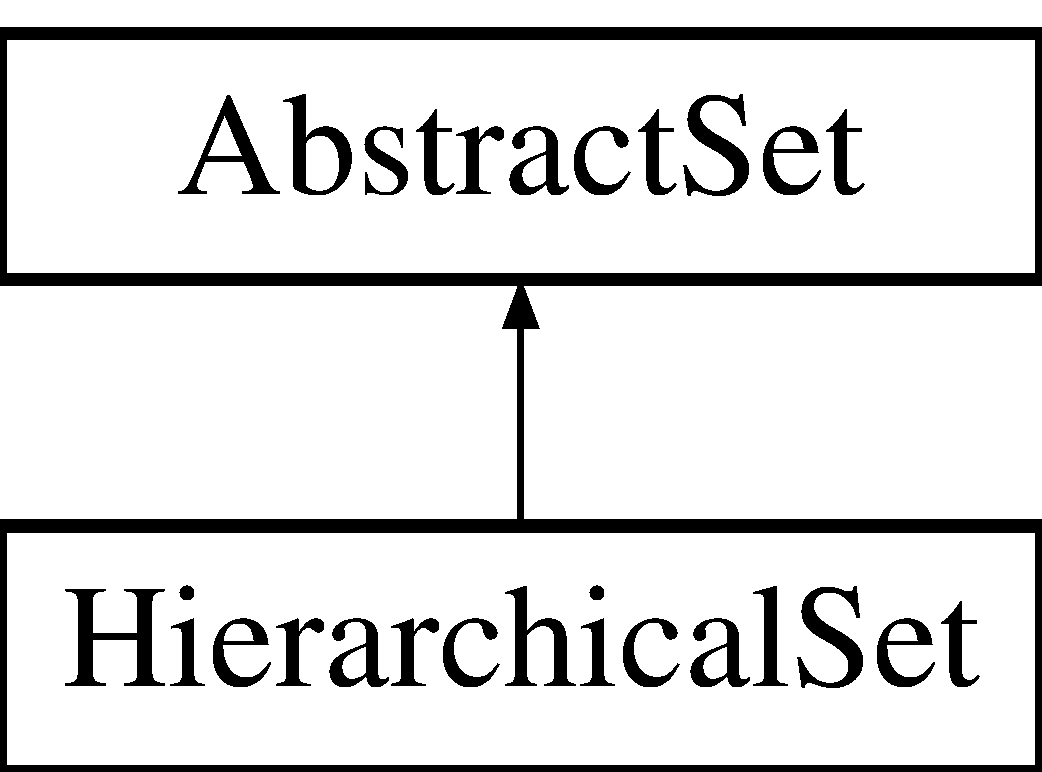
\includegraphics[height=2.000000cm]{classHierarchicalSet}
\end{center}
\end{figure}
\subsection*{Public Member Functions}
\begin{DoxyCompactItemize}
\item 
\hypertarget{classHierarchicalSet_a7fd1f8312d26ece557fface14b23cb36}{{\bfseries Hierarchical\-Set} (\hyperlink{classHNode}{H\-Node} $\ast$hierarchy)}\label{classHierarchicalSet_a7fd1f8312d26ece557fface14b23cb36}

\item 
\hypertarget{classHierarchicalSet_abccd5ddb7195f7c8941077783b7335ab}{void \hyperlink{classHierarchicalSet_abccd5ddb7195f7c8941077783b7335ab}{set\-Random} ()}\label{classHierarchicalSet_abccd5ddb7195f7c8941077783b7335ab}

\begin{DoxyCompactList}\small\item\em Randomly set the algebraic constraints for quick experiments (warning\-: this method is not always implemented) \end{DoxyCompactList}\item 
void \hyperlink{classHierarchicalSet_aa555c69a5761820567bfe391969859d3}{set\-Objective\-Function} (\hyperlink{classObjectiveFunction}{Objective\-Function} $\ast$m)
\begin{DoxyCompactList}\small\item\em Set the objective that one wants to optimise. \end{DoxyCompactList}\item 
\hypertarget{classHierarchicalSet_a6692536203bfd050a44e9abef2193564}{void \hyperlink{classHierarchicalSet_a6692536203bfd050a44e9abef2193564}{print} ()}\label{classHierarchicalSet_a6692536203bfd050a44e9abef2193564}

\begin{DoxyCompactList}\small\item\em Print the set and its algebraic constraints. \end{DoxyCompactList}\item 
\hypertarget{classHierarchicalSet_a94642b968f3cc3a8cfed07c2d4eb14ee}{void \hyperlink{classHierarchicalSet_a94642b968f3cc3a8cfed07c2d4eb14ee}{build\-Data\-Structure} ()}\label{classHierarchicalSet_a94642b968f3cc3a8cfed07c2d4eb14ee}

\begin{DoxyCompactList}\small\item\em Build a proper data structure to represent the set and its algebraic constraints (warning\-: this method should always be called after instantiating and parameterising a set, and before calling any other method, such as \hyperlink{classHierarchicalSet_a6692536203bfd050a44e9abef2193564}{print()}, \hyperlink{classHierarchicalSet_a56c3340acb36d53ec03895a2c3b4118e}{compute\-Objective\-Values()}, compute\-Optimal\-Partition (double parameter), etc.) \end{DoxyCompactList}\item 
\hypertarget{classHierarchicalSet_a56c3340acb36d53ec03895a2c3b4118e}{void \hyperlink{classHierarchicalSet_a56c3340acb36d53ec03895a2c3b4118e}{compute\-Objective\-Values} ()}\label{classHierarchicalSet_a56c3340acb36d53ec03895a2c3b4118e}

\begin{DoxyCompactList}\small\item\em Compute the value of the objective function for each feasible part (warning\-: set\-Objective\-Function (\hyperlink{classObjectiveFunction}{Objective\-Function} $\ast$objective) should have been called first) \end{DoxyCompactList}\item 
\hypertarget{classHierarchicalSet_aa0a14ba33f5942aed3f5b2901ae3821b}{void \hyperlink{classHierarchicalSet_aa0a14ba33f5942aed3f5b2901ae3821b}{normalize\-Objective\-Values} ()}\label{classHierarchicalSet_aa0a14ba33f5942aed3f5b2901ae3821b}

\begin{DoxyCompactList}\small\item\em Finish computing the value of the objective function for each feasible part when normalisation is required (warning\-: only after \hyperlink{classHierarchicalSet_a56c3340acb36d53ec03895a2c3b4118e}{compute\-Objective\-Values()} has been called) \end{DoxyCompactList}\item 
\hypertarget{classHierarchicalSet_a74c5c8512413f49efc94dd3089001867}{void \hyperlink{classHierarchicalSet_a74c5c8512413f49efc94dd3089001867}{print\-Objective\-Values} ()}\label{classHierarchicalSet_a74c5c8512413f49efc94dd3089001867}

\begin{DoxyCompactList}\small\item\em Print the value of the objective function for each feasible part. \end{DoxyCompactList}\item 
void \hyperlink{classHierarchicalSet_a98c856781a0b5e1a7d4727f0078c6838}{compute\-Optimal\-Partition} (double parameter)
\begin{DoxyCompactList}\small\item\em Compute a partition that fits with the algebraic constraints and that optimises the objective function that has been specified. \end{DoxyCompactList}\item 
void \hyperlink{classHierarchicalSet_a5cc9af69f6cf68fbfac2343207d125b5}{print\-Optimal\-Partition} (double parameter)
\begin{DoxyCompactList}\small\item\em Compute and print a partition that fits with the algebraic constraints and that optimises the objective function that has been specified (warning\-: this method is not always implemented, but one can obtain a similar result by using get\-Optimal\-Partition (double parameter) and by calling \hyperlink{classHierarchicalSet_a6692536203bfd050a44e9abef2193564}{print()} on the result) \end{DoxyCompactList}\item 
\hyperlink{classPartition}{Partition} $\ast$ \hyperlink{classHierarchicalSet_a1f7b6ed6c57f17fcdee7c7c2bfbe4925}{get\-Optimal\-Partition} (double parameter)
\begin{DoxyCompactList}\small\item\em Compute and return a partition that fits with the algebraic constraints and that optimises the objective function that has been specified (warning\-: this method is not always implemented, but one can obtain a similar result by using get\-Optimal\-Partition (double parameter) and by calling \hyperlink{classHierarchicalSet_a6692536203bfd050a44e9abef2193564}{print()} on the result) \end{DoxyCompactList}\end{DoxyCompactItemize}
\subsection*{Public Attributes}
\begin{DoxyCompactItemize}
\item 
\hypertarget{classHierarchicalSet_ab2b74de5c35a9cb3067ebe3f40c10d93}{\hyperlink{classHNode}{H\-Node} $\ast$ {\bfseries hierarchy}}\label{classHierarchicalSet_ab2b74de5c35a9cb3067ebe3f40c10d93}

\end{DoxyCompactItemize}


\subsection{Member Function Documentation}
\hypertarget{classHierarchicalSet_a98c856781a0b5e1a7d4727f0078c6838}{\index{Hierarchical\-Set@{Hierarchical\-Set}!compute\-Optimal\-Partition@{compute\-Optimal\-Partition}}
\index{compute\-Optimal\-Partition@{compute\-Optimal\-Partition}!HierarchicalSet@{Hierarchical\-Set}}
\subsubsection[{compute\-Optimal\-Partition}]{\setlength{\rightskip}{0pt plus 5cm}void Hierarchical\-Set\-::compute\-Optimal\-Partition (
\begin{DoxyParamCaption}
\item[{double}]{parameter}
\end{DoxyParamCaption}
)\hspace{0.3cm}{\ttfamily [virtual]}}}\label{classHierarchicalSet_a98c856781a0b5e1a7d4727f0078c6838}


Compute a partition that fits with the algebraic constraints and that optimises the objective function that has been specified. 


\begin{DoxyParams}{Parameters}
{\em parameter} & \-: The parameter of the objective function to be optimised (if the objective is parametrised) \\
\hline
\end{DoxyParams}


Implements \hyperlink{classAbstractSet_acfc3004f18192f38e32bb7a5a12ec8df}{Abstract\-Set}.

\hypertarget{classHierarchicalSet_a1f7b6ed6c57f17fcdee7c7c2bfbe4925}{\index{Hierarchical\-Set@{Hierarchical\-Set}!get\-Optimal\-Partition@{get\-Optimal\-Partition}}
\index{get\-Optimal\-Partition@{get\-Optimal\-Partition}!HierarchicalSet@{Hierarchical\-Set}}
\subsubsection[{get\-Optimal\-Partition}]{\setlength{\rightskip}{0pt plus 5cm}{\bf Partition} $\ast$ Hierarchical\-Set\-::get\-Optimal\-Partition (
\begin{DoxyParamCaption}
\item[{double}]{parameter}
\end{DoxyParamCaption}
)\hspace{0.3cm}{\ttfamily [virtual]}}}\label{classHierarchicalSet_a1f7b6ed6c57f17fcdee7c7c2bfbe4925}


Compute and return a partition that fits with the algebraic constraints and that optimises the objective function that has been specified (warning\-: this method is not always implemented, but one can obtain a similar result by using get\-Optimal\-Partition (double parameter) and by calling \hyperlink{classHierarchicalSet_a6692536203bfd050a44e9abef2193564}{print()} on the result) 


\begin{DoxyParams}{Parameters}
{\em parameter} & \-: The parameter of the objective function to be optimised (if the objective is parametrised) \\
\hline
\end{DoxyParams}
\begin{DoxyReturn}{Returns}
\-: The resulting optimal partition 
\end{DoxyReturn}


Implements \hyperlink{classAbstractSet_a48fd08c4b61ed46946bed6e19cd11194}{Abstract\-Set}.

\hypertarget{classHierarchicalSet_a5cc9af69f6cf68fbfac2343207d125b5}{\index{Hierarchical\-Set@{Hierarchical\-Set}!print\-Optimal\-Partition@{print\-Optimal\-Partition}}
\index{print\-Optimal\-Partition@{print\-Optimal\-Partition}!HierarchicalSet@{Hierarchical\-Set}}
\subsubsection[{print\-Optimal\-Partition}]{\setlength{\rightskip}{0pt plus 5cm}void Hierarchical\-Set\-::print\-Optimal\-Partition (
\begin{DoxyParamCaption}
\item[{double}]{parameter}
\end{DoxyParamCaption}
)\hspace{0.3cm}{\ttfamily [virtual]}}}\label{classHierarchicalSet_a5cc9af69f6cf68fbfac2343207d125b5}


Compute and print a partition that fits with the algebraic constraints and that optimises the objective function that has been specified (warning\-: this method is not always implemented, but one can obtain a similar result by using get\-Optimal\-Partition (double parameter) and by calling \hyperlink{classHierarchicalSet_a6692536203bfd050a44e9abef2193564}{print()} on the result) 


\begin{DoxyParams}{Parameters}
{\em parameter} & \-: The parameter of the objective function to be optimised (if the objective is parametrised) \\
\hline
\end{DoxyParams}


Implements \hyperlink{classAbstractSet_a82a9ce5c2d30690f0d1b83b034e92e1e}{Abstract\-Set}.

\hypertarget{classHierarchicalSet_aa555c69a5761820567bfe391969859d3}{\index{Hierarchical\-Set@{Hierarchical\-Set}!set\-Objective\-Function@{set\-Objective\-Function}}
\index{set\-Objective\-Function@{set\-Objective\-Function}!HierarchicalSet@{Hierarchical\-Set}}
\subsubsection[{set\-Objective\-Function}]{\setlength{\rightskip}{0pt plus 5cm}void Hierarchical\-Set\-::set\-Objective\-Function (
\begin{DoxyParamCaption}
\item[{{\bf Objective\-Function} $\ast$}]{objective}
\end{DoxyParamCaption}
)\hspace{0.3cm}{\ttfamily [virtual]}}}\label{classHierarchicalSet_aa555c69a5761820567bfe391969859d3}


Set the objective that one wants to optimise. 


\begin{DoxyParams}{Parameters}
{\em objective} & \-: The objective function itself \\
\hline
\end{DoxyParams}


Implements \hyperlink{classAbstractSet_a7aef71679a18ab7965d1098da15b26c2}{Abstract\-Set}.



The documentation for this class was generated from the following files\-:\begin{DoxyCompactItemize}
\item 
src/hierarchical\-\_\-set.\-hpp\item 
src/hierarchical\-\_\-set.\-cpp\end{DoxyCompactItemize}

\hypertarget{classHierarchicalStructure}{\section{Hierarchical\-Structure Class Reference}
\label{classHierarchicalStructure}\index{Hierarchical\-Structure@{Hierarchical\-Structure}}
}
Inheritance diagram for Hierarchical\-Structure\-:\begin{figure}[H]
\begin{center}
\leavevmode
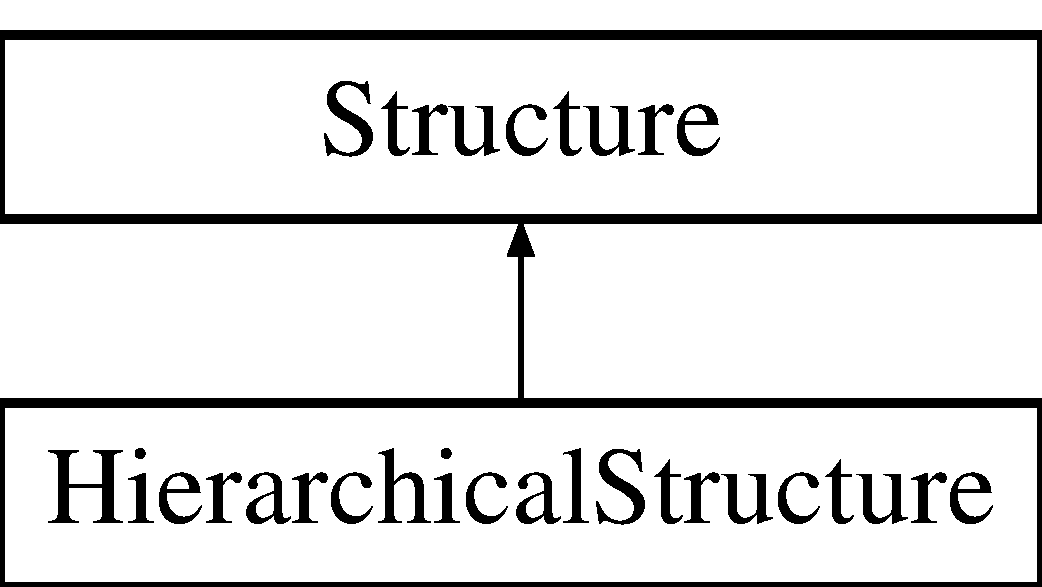
\includegraphics[height=2.000000cm]{classHierarchicalStructure}
\end{center}
\end{figure}
\subsection*{Public Member Functions}
\begin{DoxyCompactItemize}
\item 
\hypertarget{classHierarchicalStructure_af890848efff872a4da793f041a026c62}{{\bfseries Hierarchical\-Structure} (int depth)}\label{classHierarchicalStructure_af890848efff872a4da793f041a026c62}

\item 
\hypertarget{classHierarchicalStructure_a23422af4415e39de39e577ddd82ac4d9}{int {\bfseries build\-Hierarchy} (\hyperlink{classAggregate}{Aggregate} $\ast$aggregate, int depth, int index)}\label{classHierarchicalStructure_a23422af4415e39de39e577ddd82ac4d9}

\end{DoxyCompactItemize}
\subsection*{Public Attributes}
\begin{DoxyCompactItemize}
\item 
\hypertarget{classHierarchicalStructure_a8f6d2b5b65b1fda6257e6d25362ad766}{int {\bfseries depth}}\label{classHierarchicalStructure_a8f6d2b5b65b1fda6257e6d25362ad766}

\end{DoxyCompactItemize}


The documentation for this class was generated from the following files\-:\begin{DoxyCompactItemize}
\item 
/home/lamarche/programming/optimal\-\_\-partition/src/structure.\-hpp\item 
/home/lamarche/programming/optimal\-\_\-partition/src/structure.\-cpp\end{DoxyCompactItemize}

\hypertarget{classHNode}{\section{H\-Node Class Reference}
\label{classHNode}\index{H\-Node@{H\-Node}}
}
\subsection*{Public Member Functions}
\begin{DoxyCompactItemize}
\item 
\hypertarget{classHNode_abdd79609f34c6318445bc4dee03f34d2}{{\bfseries H\-Node} (int index=-\/1)}\label{classHNode_abdd79609f34c6318445bc4dee03f34d2}

\item 
\hypertarget{classHNode_ad17d7be7f28d433db5d7c1b8f61aca39}{void {\bfseries add\-Child} (\hyperlink{classHNode}{H\-Node} $\ast$node)}\label{classHNode_ad17d7be7f28d433db5d7c1b8f61aca39}

\item 
\hypertarget{classHNode_a829d5b0388867bff02e414f73c545ea0}{void {\bfseries set\-Objective\-Function} (\hyperlink{classObjectiveFunction}{Objective\-Function} $\ast$m)}\label{classHNode_a829d5b0388867bff02e414f73c545ea0}

\item 
\hypertarget{classHNode_a00d9c439d12421fda1aecfd06411d4ec}{void {\bfseries print} ()}\label{classHNode_a00d9c439d12421fda1aecfd06411d4ec}

\item 
\hypertarget{classHNode_ad5c92795c03295d891545d435cf4ea64}{void {\bfseries print\-Indices} (bool endl=false)}\label{classHNode_ad5c92795c03295d891545d435cf4ea64}

\item 
\hypertarget{classHNode_a05fa5672b3c4dde3a8b9686ee91aca2f}{void {\bfseries build\-Data\-Structure} (\hyperlink{classHNode}{H\-Node} $\ast$root=0, int level=0, int num=0)}\label{classHNode_a05fa5672b3c4dde3a8b9686ee91aca2f}

\item 
\hypertarget{classHNode_a405e9125ac0e08eb6e05a8743ca5be86}{void {\bfseries compute\-Objective\-Values} ()}\label{classHNode_a405e9125ac0e08eb6e05a8743ca5be86}

\item 
\hypertarget{classHNode_a805a676e4362d92aa61947792b5b6afa}{void {\bfseries normalize\-Objective\-Values} (\hyperlink{classObjectiveValue}{Objective\-Value} $\ast$max\-Qual=0)}\label{classHNode_a805a676e4362d92aa61947792b5b6afa}

\item 
\hypertarget{classHNode_a2b772372f36d2326c1d20d207f256f0a}{void {\bfseries print\-Objective\-Values} ()}\label{classHNode_a2b772372f36d2326c1d20d207f256f0a}

\item 
\hypertarget{classHNode_a074ae5b775ec9045d421492340a19275}{void {\bfseries compute\-Optimal\-Partition} (double parameter)}\label{classHNode_a074ae5b775ec9045d421492340a19275}

\item 
\hypertarget{classHNode_a4e1c467904bc2d18bcead37dac9a19dd}{void {\bfseries print\-Optimal\-Partition} (double parameter)}\label{classHNode_a4e1c467904bc2d18bcead37dac9a19dd}

\item 
\hypertarget{classHNode_aba01cb91eaeba4e7da47069d519275f7}{\hyperlink{classPartition}{Partition} $\ast$ {\bfseries get\-Optimal\-Partition} (double parameter)}\label{classHNode_aba01cb91eaeba4e7da47069d519275f7}

\item 
\hypertarget{classHNode_ad6bbcff7cf7d713bc1d554561d288f47}{void {\bfseries build\-Optimal\-Partition} (\hyperlink{classPartition}{Partition} $\ast$partition)}\label{classHNode_ad6bbcff7cf7d713bc1d554561d288f47}

\end{DoxyCompactItemize}
\subsection*{Public Attributes}
\begin{DoxyCompactItemize}
\item 
\hypertarget{classHNode_a5e2c6cb9918a764753952cdd28617570}{int {\bfseries index}}\label{classHNode_a5e2c6cb9918a764753952cdd28617570}

\item 
\hypertarget{classHNode_a2dc355d3d7502bb90e8682bd81087575}{std\-::set$<$ int $>$ $\ast$ {\bfseries indices}}\label{classHNode_a2dc355d3d7502bb90e8682bd81087575}

\item 
\hypertarget{classHNode_adcc11fe69c64eeb77f920b98e404d9e9}{int {\bfseries level}}\label{classHNode_adcc11fe69c64eeb77f920b98e404d9e9}

\item 
\hypertarget{classHNode_a647c6437fde5eccdfab4879b7c485707}{int {\bfseries size}}\label{classHNode_a647c6437fde5eccdfab4879b7c485707}

\item 
\hypertarget{classHNode_a5bdb5568025a03c7f96cf638821f655d}{int {\bfseries width}}\label{classHNode_a5bdb5568025a03c7f96cf638821f655d}

\item 
\hypertarget{classHNode_a80af2cfac18d728df6f581385fafbb2e}{int {\bfseries num}}\label{classHNode_a80af2cfac18d728df6f581385fafbb2e}

\item 
\hypertarget{classHNode_ad1fc63b85babb8d83f3be87468210e32}{\hyperlink{classHNode}{H\-Node} $\ast$ {\bfseries root}}\label{classHNode_ad1fc63b85babb8d83f3be87468210e32}

\item 
\hypertarget{classHNode_a9138b7f3a2168c03aebc5893364c576f}{H\-Node\-Set $\ast$ {\bfseries children}}\label{classHNode_a9138b7f3a2168c03aebc5893364c576f}

\item 
\hypertarget{classHNode_a7e4827e4c414093a839240472d05f073}{\hyperlink{classObjectiveFunction}{Objective\-Function} $\ast$ {\bfseries objective}}\label{classHNode_a7e4827e4c414093a839240472d05f073}

\item 
\hypertarget{classHNode_aa2362c0c68e9992a9d9c33e7f8523fe0}{\hyperlink{classObjectiveValue}{Objective\-Value} $\ast$ {\bfseries value}}\label{classHNode_aa2362c0c68e9992a9d9c33e7f8523fe0}

\item 
\hypertarget{classHNode_a01f5c59e976223a8561676b427fe4125}{double {\bfseries optimal\-Value}}\label{classHNode_a01f5c59e976223a8561676b427fe4125}

\item 
\hypertarget{classHNode_a08d0d33f51f8d7d96852e9a022af93f3}{bool {\bfseries optimal\-Cut}}\label{classHNode_a08d0d33f51f8d7d96852e9a022af93f3}

\end{DoxyCompactItemize}


The documentation for this class was generated from the following files\-:\begin{DoxyCompactItemize}
\item 
/home/lamarche/programming/optimal\-\_\-partition/src/hierarchical\-\_\-set.\-hpp\item 
/home/lamarche/programming/optimal\-\_\-partition/src/hierarchical\-\_\-set.\-cpp\end{DoxyCompactItemize}

\hypertarget{classHONode}{\section{H\-O\-Node Class Reference}
\label{classHONode}\index{H\-O\-Node@{H\-O\-Node}}
}
\subsection*{Public Member Functions}
\begin{DoxyCompactItemize}
\item 
\hypertarget{classHONode_a9aede08d7bddc624967aa4507a7321e2}{{\bfseries H\-O\-Node} (int size, int index=-\/1)}\label{classHONode_a9aede08d7bddc624967aa4507a7321e2}

\item 
\hypertarget{classHONode_ab0ee2ebf84a8f000307814d8a00c08d9}{int {\bfseries get\-Index} (int i, int j)}\label{classHONode_ab0ee2ebf84a8f000307814d8a00c08d9}

\item 
\hypertarget{classHONode_adae5c176d67b8987aa1d15c34452630c}{void {\bfseries add\-Child} (\hyperlink{classHONode}{H\-O\-Node} $\ast$node)}\label{classHONode_adae5c176d67b8987aa1d15c34452630c}

\item 
\hypertarget{classHONode_a2bc5353bc6ee8a94205d750275ffc075}{void {\bfseries set\-Objective\-Function} (\hyperlink{classObjectiveFunction}{Objective\-Function} $\ast$m)}\label{classHONode_a2bc5353bc6ee8a94205d750275ffc075}

\item 
\hypertarget{classHONode_ad877ce2e3b922508dc854c485abc34cf}{void {\bfseries print} ()}\label{classHONode_ad877ce2e3b922508dc854c485abc34cf}

\item 
\hypertarget{classHONode_a3c1d16d6337081b35de83af5c743bb51}{void {\bfseries build\-Data\-Structure} (int level=0)}\label{classHONode_a3c1d16d6337081b35de83af5c743bb51}

\item 
\hypertarget{classHONode_aa92d038a2def42f2ee9cb73dfbc422da}{void {\bfseries compute\-Objective\-Values} ()}\label{classHONode_aa92d038a2def42f2ee9cb73dfbc422da}

\item 
\hypertarget{classHONode_a1f780e020ab5150d27bb04a96af13133}{void {\bfseries normalize\-Objective\-Values} (\hyperlink{classObjectiveValue}{Objective\-Value} $\ast$max\-Qual=0)}\label{classHONode_a1f780e020ab5150d27bb04a96af13133}

\item 
\hypertarget{classHONode_a5ec6f4b4c9313d372282114af15d0a6d}{void {\bfseries print\-Objective\-Values} ()}\label{classHONode_a5ec6f4b4c9313d372282114af15d0a6d}

\item 
\hypertarget{classHONode_a1ede3a94ec46b81b2250874a6dcefb98}{void {\bfseries compute\-Optimal\-Partition} (double parameter)}\label{classHONode_a1ede3a94ec46b81b2250874a6dcefb98}

\item 
\hypertarget{classHONode_a9a4df13c77c8ab4b541446d3b3b4cacd}{void {\bfseries print\-Optimal\-Partition} (double parameter)}\label{classHONode_a9a4df13c77c8ab4b541446d3b3b4cacd}

\item 
\hypertarget{classHONode_af2905a01a848793e8614beb12bb62df8}{\hyperlink{classPartition}{Partition} $\ast$ {\bfseries get\-Optimal\-Partition} (double parameter)}\label{classHONode_af2905a01a848793e8614beb12bb62df8}

\item 
\hypertarget{classHONode_abfd6c5724bd46fd91c6537554e9d4d1b}{void {\bfseries build\-Optimal\-Partition} (\hyperlink{classPartition}{Partition} $\ast$partition, int pi=0, int pj=-\/1)}\label{classHONode_abfd6c5724bd46fd91c6537554e9d4d1b}

\end{DoxyCompactItemize}
\subsection*{Public Attributes}
\begin{DoxyCompactItemize}
\item 
\hypertarget{classHONode_afdceeb6b9dd641633be6b81380b9bb0f}{int {\bfseries index}}\label{classHONode_afdceeb6b9dd641633be6b81380b9bb0f}

\item 
\hypertarget{classHONode_ae8d4dd48892372be94f6e214450c5e44}{int {\bfseries level}}\label{classHONode_ae8d4dd48892372be94f6e214450c5e44}

\item 
\hypertarget{classHONode_a8d093f3290293ea7b7e03a185798fe64}{std\-::set$<$ int $>$ $\ast$ {\bfseries indices}}\label{classHONode_a8d093f3290293ea7b7e03a185798fe64}

\item 
\hypertarget{classHONode_a1c4e4ef9ffa03161b427606cd6255b52}{H\-O\-Node\-Set $\ast$ {\bfseries children}}\label{classHONode_a1c4e4ef9ffa03161b427606cd6255b52}

\item 
\hypertarget{classHONode_a3fd5dd67e556117b39d50412718f47e4}{\hyperlink{classObjectiveFunction}{Objective\-Function} $\ast$ {\bfseries objective}}\label{classHONode_a3fd5dd67e556117b39d50412718f47e4}

\item 
\hypertarget{classHONode_ad63d56300726c5d89d11276ab1c3fdec}{int {\bfseries size}}\label{classHONode_ad63d56300726c5d89d11276ab1c3fdec}

\item 
\hypertarget{classHONode_acf196983ba89362f7509dbf1758513d3}{\hyperlink{classObjectiveValue}{Objective\-Value} $\ast$$\ast$ {\bfseries qualities}}\label{classHONode_acf196983ba89362f7509dbf1758513d3}

\item 
\hypertarget{classHONode_af9e4cf35f08fe3c9d4ec44cabc1d439d}{double $\ast$ {\bfseries optimal\-Values}}\label{classHONode_af9e4cf35f08fe3c9d4ec44cabc1d439d}

\item 
\hypertarget{classHONode_ac2b2e15ed1a6893c073d2551c735b2d2}{int $\ast$ {\bfseries optimal\-Cuts}}\label{classHONode_ac2b2e15ed1a6893c073d2551c735b2d2}

\end{DoxyCompactItemize}


The documentation for this class was generated from the following files\-:\begin{DoxyCompactItemize}
\item 
src/hierarchical\-\_\-ordered\-\_\-set.\-hpp\item 
src/hierarchical\-\_\-ordered\-\_\-set.\-cpp\end{DoxyCompactItemize}

\hypertarget{classHyperAggregate}{\section{Hyper\-Aggregate Class Reference}
\label{classHyperAggregate}\index{Hyper\-Aggregate@{Hyper\-Aggregate}}
}
\subsection*{Public Member Functions}
\begin{DoxyCompactItemize}
\item 
\hypertarget{classHyperAggregate_a07b89e7c22ffeb5021707f1c3ef821f6}{{\bfseries Hyper\-Aggregate} (\hyperlink{classAggregate}{Aggregate} $\ast$$\ast$aggregate\-Array, int dimension)}\label{classHyperAggregate_a07b89e7c22ffeb5021707f1c3ef821f6}

\item 
\hypertarget{classHyperAggregate_a189540a613a9a27c4c458a3b0febf974}{void {\bfseries print} ()}\label{classHyperAggregate_a189540a613a9a27c4c458a3b0febf974}

\item 
\hypertarget{classHyperAggregate_ad01f17867baea2abe0d2d51407d604ac}{void {\bfseries print\-Index\-Set} (bool endl=false)}\label{classHyperAggregate_ad01f17867baea2abe0d2d51407d604ac}

\item 
\hypertarget{classHyperAggregate_a8e03ce6d7669702d6b78e4ef5b7a1b64}{void {\bfseries add\-Aggregate\-Set} (Hyper\-Aggregate\-Set $\ast$aggregate\-Set)}\label{classHyperAggregate_a8e03ce6d7669702d6b78e4ef5b7a1b64}

\item 
\hypertarget{classHyperAggregate_a457a4455a692bd49510937281634f649}{void {\bfseries set\-Objective\-Function} (\hyperlink{classObjectiveFunction}{Objective\-Function} $\ast$m)}\label{classHyperAggregate_a457a4455a692bd49510937281634f649}

\item 
\hypertarget{classHyperAggregate_ade2f5042664cd52a541fb7e1cf516d19}{void {\bfseries build\-Data\-Structure} ()}\label{classHyperAggregate_ade2f5042664cd52a541fb7e1cf516d19}

\item 
\hypertarget{classHyperAggregate_a82f62a9329d38b8636aad039e528599c}{void {\bfseries compute\-Objective\-Values} ()}\label{classHyperAggregate_a82f62a9329d38b8636aad039e528599c}

\item 
\hypertarget{classHyperAggregate_acf16618e534c7df803894d8961e0832a}{void {\bfseries normalize\-Objective\-Values} (\hyperlink{classObjectiveValue}{Objective\-Value} $\ast$max\-Qual=0)}\label{classHyperAggregate_acf16618e534c7df803894d8961e0832a}

\item 
\hypertarget{classHyperAggregate_a91272c9cf49b90bc4846c700239d4e89}{void {\bfseries print\-Objective\-Values} ()}\label{classHyperAggregate_a91272c9cf49b90bc4846c700239d4e89}

\item 
\hypertarget{classHyperAggregate_aef37d4223c7ba9a11c5a7caffecdb135}{void {\bfseries compute\-Optimal\-Partition} (double parameter)}\label{classHyperAggregate_aef37d4223c7ba9a11c5a7caffecdb135}

\item 
\hypertarget{classHyperAggregate_aeaa20e17ecd99774566d29bb9cd18d51}{void {\bfseries print\-Optimal\-Partition} (double parameter)}\label{classHyperAggregate_aeaa20e17ecd99774566d29bb9cd18d51}

\item 
\hypertarget{classHyperAggregate_a1ea6a32acd88afe438fcee9dcaeb0103}{void {\bfseries build\-Optimal\-Partition} (\hyperlink{classPartition}{Partition} $\ast$partition)}\label{classHyperAggregate_a1ea6a32acd88afe438fcee9dcaeb0103}

\end{DoxyCompactItemize}
\subsection*{Public Attributes}
\begin{DoxyCompactItemize}
\item 
\hypertarget{classHyperAggregate_a4d83d2c954e243ea4427563a601d60c6}{int {\bfseries dimension}}\label{classHyperAggregate_a4d83d2c954e243ea4427563a601d60c6}

\item 
\hypertarget{classHyperAggregate_a918e4c93b5f3c2da1a982ef7cc51297f}{\hyperlink{classAggregate}{Aggregate} $\ast$$\ast$ {\bfseries aggregate\-Array}}\label{classHyperAggregate_a918e4c93b5f3c2da1a982ef7cc51297f}

\item 
\hypertarget{classHyperAggregate_ac7fca59b15740a76f95bbc2a490f954f}{int {\bfseries num}}\label{classHyperAggregate_ac7fca59b15740a76f95bbc2a490f954f}

\item 
\hypertarget{classHyperAggregate_aeff461b2ab34f107505469b0fbe4a580}{int {\bfseries atomic\-Num}}\label{classHyperAggregate_aeff461b2ab34f107505469b0fbe4a580}

\item 
\hypertarget{classHyperAggregate_a49a8f6fbf66994f023141ad53d756c3e}{bool {\bfseries is\-Atomic}}\label{classHyperAggregate_a49a8f6fbf66994f023141ad53d756c3e}

\item 
\hypertarget{classHyperAggregate_a61bd0e802b8e3fa3792b03f75d035d97}{bool {\bfseries reached}}\label{classHyperAggregate_a61bd0e802b8e3fa3792b03f75d035d97}

\item 
\hypertarget{classHyperAggregate_ae024a1f7a8a9e16e18cfc08157d78067}{Hyper\-Aggregate\-Set\-Set $\ast$ {\bfseries aggregate\-Set\-Set}}\label{classHyperAggregate_ae024a1f7a8a9e16e18cfc08157d78067}

\item 
\hypertarget{classHyperAggregate_a904499d5fd048c8279babe1007a9f526}{\hyperlink{classHyperStructure}{Hyper\-Structure} $\ast$ {\bfseries structure}}\label{classHyperAggregate_a904499d5fd048c8279babe1007a9f526}

\item 
\hypertarget{classHyperAggregate_a20f30b86f34c47baf737da2f1dd3528f}{\hyperlink{classObjectiveFunction}{Objective\-Function} $\ast$ {\bfseries objective}}\label{classHyperAggregate_a20f30b86f34c47baf737da2f1dd3528f}

\item 
\hypertarget{classHyperAggregate_a35e1fe6c4eef7996e4c3ad70534f8a0b}{\hyperlink{classObjectiveValue}{Objective\-Value} $\ast$ {\bfseries value}}\label{classHyperAggregate_a35e1fe6c4eef7996e4c3ad70534f8a0b}

\item 
\hypertarget{classHyperAggregate_a6e1560f410a9038d03ee4a1aefb482f5}{double {\bfseries optimal\-Value}}\label{classHyperAggregate_a6e1560f410a9038d03ee4a1aefb482f5}

\item 
\hypertarget{classHyperAggregate_a5e3aa280f0a438a085a61847d8299a92}{Hyper\-Aggregate\-Set $\ast$ {\bfseries optimal\-Cut}}\label{classHyperAggregate_a5e3aa280f0a438a085a61847d8299a92}

\end{DoxyCompactItemize}


The documentation for this class was generated from the following files\-:\begin{DoxyCompactItemize}
\item 
/home/lamarche/programming/optimal\-\_\-partition/src/hyper\-\_\-structure.\-hpp\item 
/home/lamarche/programming/optimal\-\_\-partition/src/hyper\-\_\-structure.\-cpp\end{DoxyCompactItemize}

\hypertarget{classHyperPart}{\section{Hyper\-Part Class Reference}
\label{classHyperPart}\index{Hyper\-Part@{Hyper\-Part}}
}
Inheritance diagram for Hyper\-Part\-:\begin{figure}[H]
\begin{center}
\leavevmode
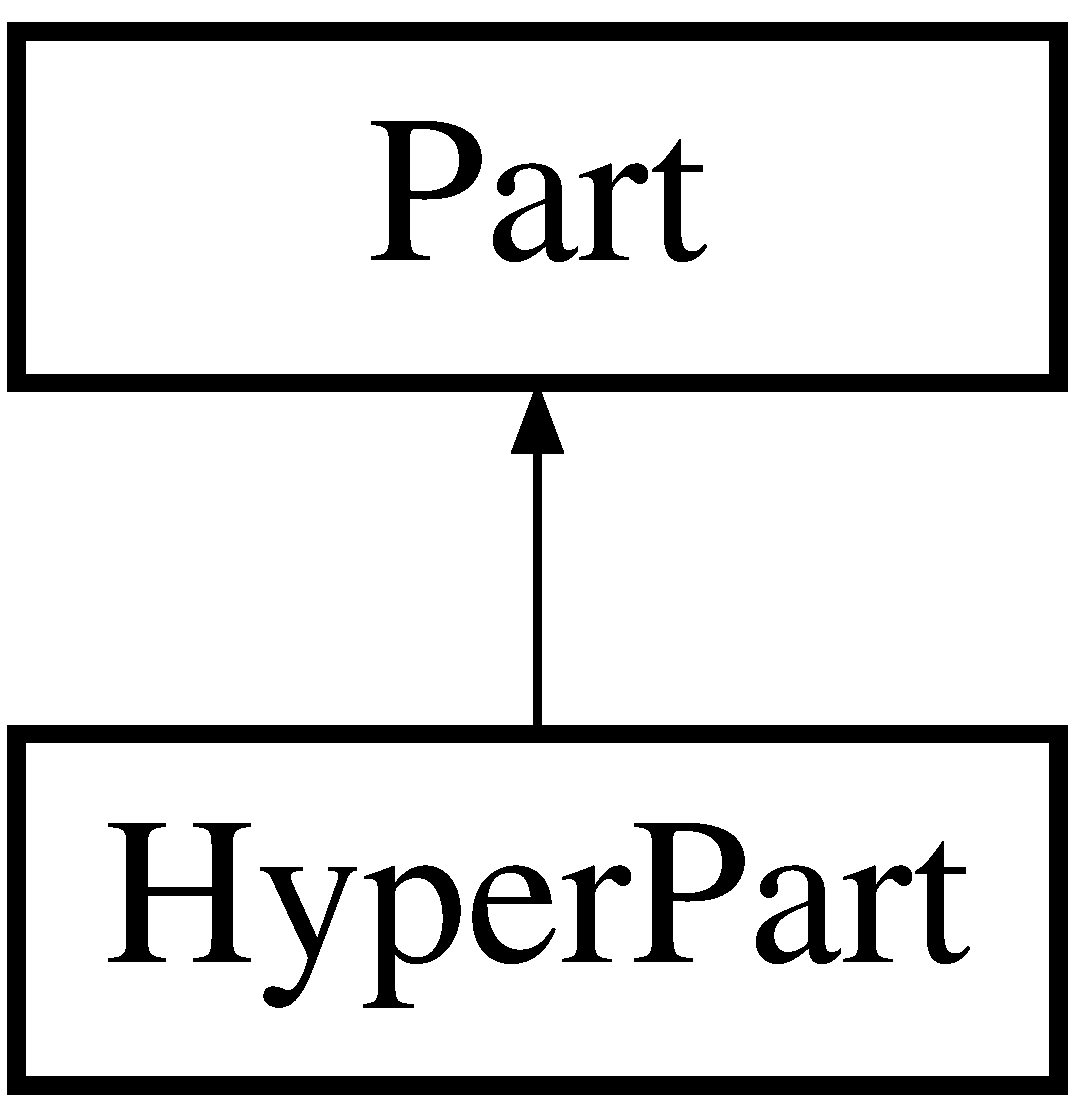
\includegraphics[height=2.000000cm]{classHyperPart}
\end{center}
\end{figure}
\subsection*{Public Member Functions}
\begin{DoxyCompactItemize}
\item 
\hypertarget{classHyperPart_afe8afb46a961a23cfcb05a54089cd52f}{{\bfseries Hyper\-Part} (\hyperlink{classPart}{Part} $\ast$$\ast$part\-Array, int dimension, \hyperlink{classObjectiveValue}{Objective\-Value} $\ast$value=0)}\label{classHyperPart_afe8afb46a961a23cfcb05a54089cd52f}

\item 
\hypertarget{classHyperPart_ab3a0e54e5c9d3874daed4d214c093108}{{\bfseries Hyper\-Part} (\hyperlink{classHyperPart}{Hyper\-Part} $\ast$hyper\-Part)}\label{classHyperPart_ab3a0e54e5c9d3874daed4d214c093108}

\item 
\hypertarget{classHyperPart_acfd0161a91999f09dc3f6f6ea871d212}{bool {\bfseries equal} (\hyperlink{classPart}{Part} $\ast$p)}\label{classHyperPart_acfd0161a91999f09dc3f6f6ea871d212}

\item 
\hypertarget{classHyperPart_a3be34de84de996312ad865cec5c647aa}{void {\bfseries print} (bool endl=false)}\label{classHyperPart_a3be34de84de996312ad865cec5c647aa}

\item 
\hypertarget{classHyperPart_a38e7c95cac44dc9048e24ef24e069f07}{int {\bfseries print\-Size} ()}\label{classHyperPart_a38e7c95cac44dc9048e24ef24e069f07}

\end{DoxyCompactItemize}
\subsection*{Public Attributes}
\begin{DoxyCompactItemize}
\item 
\hypertarget{classHyperPart_a6563c05d359489690b7d98a886bbd856}{int {\bfseries dimension}}\label{classHyperPart_a6563c05d359489690b7d98a886bbd856}

\item 
\hypertarget{classHyperPart_a6aae7e066a66fdb1ef427ce763bc0ce3}{\hyperlink{classPart}{Part} $\ast$$\ast$ {\bfseries part\-Array}}\label{classHyperPart_a6aae7e066a66fdb1ef427ce763bc0ce3}

\end{DoxyCompactItemize}


The documentation for this class was generated from the following files\-:\begin{DoxyCompactItemize}
\item 
/home/lamarche/programming/optimal\-\_\-partition/src/partition.\-hpp\item 
/home/lamarche/programming/optimal\-\_\-partition/src/partition.\-cpp\end{DoxyCompactItemize}

\hypertarget{classHyperStructure}{\section{Hyper\-Structure Class Reference}
\label{classHyperStructure}\index{Hyper\-Structure@{Hyper\-Structure}}
}
Inheritance diagram for Hyper\-Structure\-:\begin{figure}[H]
\begin{center}
\leavevmode
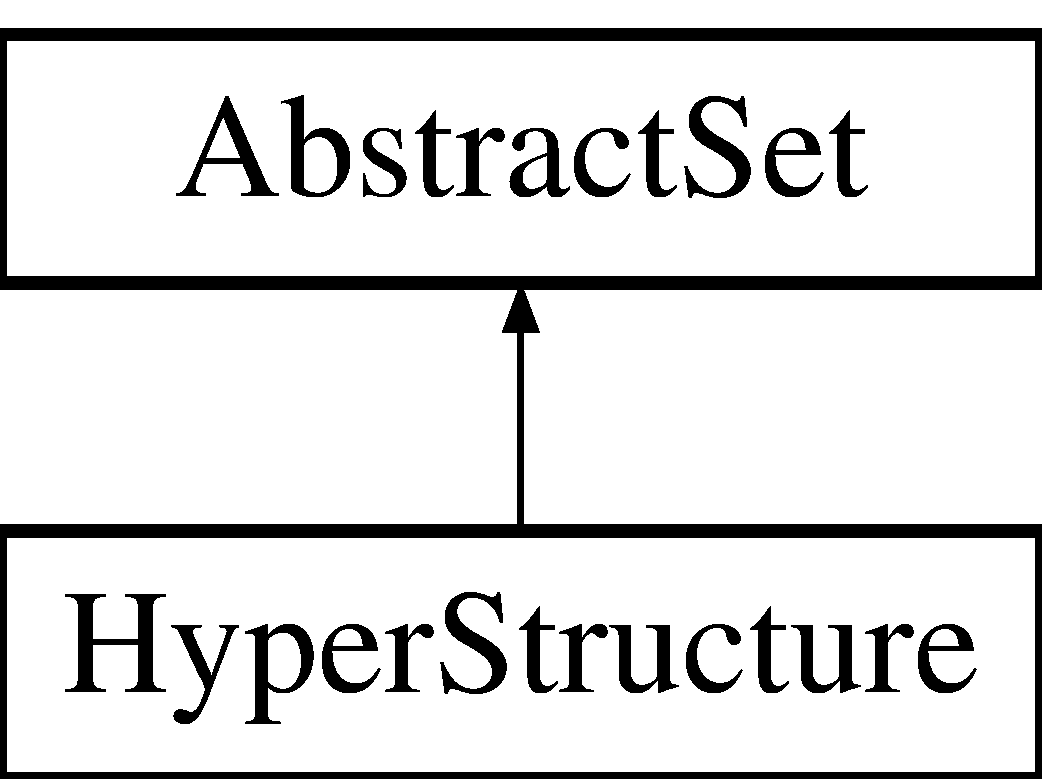
\includegraphics[height=2.000000cm]{classHyperStructure}
\end{center}
\end{figure}
\subsection*{Public Member Functions}
\begin{DoxyCompactItemize}
\item 
\hypertarget{classHyperStructure_a339a85f5da6decaccf7b517be1edbdca}{{\bfseries Hyper\-Structure} (\hyperlink{classStructure}{Structure} $\ast$structure)}\label{classHyperStructure_a339a85f5da6decaccf7b517be1edbdca}

\item 
\hypertarget{classHyperStructure_a6b5bc3c7e8c72b8dc69ea8bc191e2b45}{{\bfseries Hyper\-Structure} (\hyperlink{classStructure}{Structure} $\ast$$\ast$structure\-Array, int dimension)}\label{classHyperStructure_a6b5bc3c7e8c72b8dc69ea8bc191e2b45}

\item 
\hypertarget{classHyperStructure_ad054fc169f65693d2cd01a3b5fc0b1db}{int {\bfseries get\-Num} (int $\ast$hyper\-Num)}\label{classHyperStructure_ad054fc169f65693d2cd01a3b5fc0b1db}

\item 
\hypertarget{classHyperStructure_a9f10f159ec5828ef487265ae3473d95a}{int $\ast$ {\bfseries get\-Hyper\-Num} (int num)}\label{classHyperStructure_a9f10f159ec5828ef487265ae3473d95a}

\item 
\hypertarget{classHyperStructure_a947dcb1deb7679b8d68e91c28645a148}{\hyperlink{classHyperAggregate}{Hyper\-Aggregate} $\ast$ {\bfseries get\-Atomic\-Aggregate} (int index)}\label{classHyperStructure_a947dcb1deb7679b8d68e91c28645a148}

\item 
\hypertarget{classHyperStructure_a90f669ef93b94ed7bd4b0d04aa351c4c}{void {\bfseries init\-Reached} ()}\label{classHyperStructure_a90f669ef93b94ed7bd4b0d04aa351c4c}

\item 
\hypertarget{classHyperStructure_a39f186557c9e0e9207103d51ab03dd0d}{void \hyperlink{classHyperStructure_a39f186557c9e0e9207103d51ab03dd0d}{set\-Random} ()}\label{classHyperStructure_a39f186557c9e0e9207103d51ab03dd0d}

\begin{DoxyCompactList}\small\item\em Randomly set the algebraic constraints for quick experiments (warning\-: this method is not always implemented) \end{DoxyCompactList}\item 
void \hyperlink{classHyperStructure_a744a8c5b7bf67dec8084c5d2b8a4927d}{set\-Objective\-Function} (\hyperlink{classObjectiveFunction}{Objective\-Function} $\ast$m)
\begin{DoxyCompactList}\small\item\em Set the objective that one wants to optimise. \end{DoxyCompactList}\item 
\hypertarget{classHyperStructure_ae2c9f70f3b85cde571fdcf06b7ae08ea}{void \hyperlink{classHyperStructure_ae2c9f70f3b85cde571fdcf06b7ae08ea}{print} ()}\label{classHyperStructure_ae2c9f70f3b85cde571fdcf06b7ae08ea}

\begin{DoxyCompactList}\small\item\em Print the set and its algebraic constraints. \end{DoxyCompactList}\item 
\hypertarget{classHyperStructure_a6ad130df72d4ea8133c269ec898d51fa}{void \hyperlink{classHyperStructure_a6ad130df72d4ea8133c269ec898d51fa}{build\-Data\-Structure} ()}\label{classHyperStructure_a6ad130df72d4ea8133c269ec898d51fa}

\begin{DoxyCompactList}\small\item\em Build a proper data structure to represent the set and its algebraic constraints (warning\-: this method should always be called after instantiating and parameterising a set, and before calling any other method, such as \hyperlink{classHyperStructure_ae2c9f70f3b85cde571fdcf06b7ae08ea}{print()}, \hyperlink{classHyperStructure_a7548fc87c5e85830226ecdbadb5d4380}{compute\-Objective\-Values()}, compute\-Optimal\-Partition (double parameter), etc.) \end{DoxyCompactList}\item 
\hypertarget{classHyperStructure_a7548fc87c5e85830226ecdbadb5d4380}{void \hyperlink{classHyperStructure_a7548fc87c5e85830226ecdbadb5d4380}{compute\-Objective\-Values} ()}\label{classHyperStructure_a7548fc87c5e85830226ecdbadb5d4380}

\begin{DoxyCompactList}\small\item\em Compute the value of the objective function for each feasible part (warning\-: set\-Objective\-Function (\hyperlink{classObjectiveFunction}{Objective\-Function} $\ast$objective) should have been called first) \end{DoxyCompactList}\item 
\hypertarget{classHyperStructure_aafb180a73ba1ce8986a2c4a8dbac85cb}{void \hyperlink{classHyperStructure_aafb180a73ba1ce8986a2c4a8dbac85cb}{normalize\-Objective\-Values} ()}\label{classHyperStructure_aafb180a73ba1ce8986a2c4a8dbac85cb}

\begin{DoxyCompactList}\small\item\em Finish computing the value of the objective function for each feasible part when normalisation is required (warning\-: only after \hyperlink{classHyperStructure_a7548fc87c5e85830226ecdbadb5d4380}{compute\-Objective\-Values()} has been called) \end{DoxyCompactList}\item 
\hypertarget{classHyperStructure_ab408a372347d5c6683637a30900e5a6c}{void \hyperlink{classHyperStructure_ab408a372347d5c6683637a30900e5a6c}{print\-Objective\-Values} ()}\label{classHyperStructure_ab408a372347d5c6683637a30900e5a6c}

\begin{DoxyCompactList}\small\item\em Print the value of the objective function for each feasible part. \end{DoxyCompactList}\item 
void \hyperlink{classHyperStructure_a22374eb5de711c6ded42c439fec90711}{compute\-Optimal\-Partition} (double parameter)
\begin{DoxyCompactList}\small\item\em Compute a partition that fits with the algebraic constraints and that optimises the objective function that has been specified. \end{DoxyCompactList}\item 
void \hyperlink{classHyperStructure_af96b6f648e4aa1459ae1c8d61352413c}{print\-Optimal\-Partition} (double parameter)
\begin{DoxyCompactList}\small\item\em Compute and print a partition that fits with the algebraic constraints and that optimises the objective function that has been specified (warning\-: this method is not always implemented, but one can obtain a similar result by using get\-Optimal\-Partition (double parameter) and by calling \hyperlink{classHyperStructure_ae2c9f70f3b85cde571fdcf06b7ae08ea}{print()} on the result) \end{DoxyCompactList}\item 
\hyperlink{classPartition}{Partition} $\ast$ \hyperlink{classHyperStructure_a36cc3358d624e945de2946d7d706c6a2}{get\-Optimal\-Partition} (double parameter)
\begin{DoxyCompactList}\small\item\em Compute and return a partition that fits with the algebraic constraints and that optimises the objective function that has been specified (warning\-: this method is not always implemented, but one can obtain a similar result by using get\-Optimal\-Partition (double parameter) and by calling \hyperlink{classHyperStructure_ae2c9f70f3b85cde571fdcf06b7ae08ea}{print()} on the result) \end{DoxyCompactList}\end{DoxyCompactItemize}
\subsection*{Public Attributes}
\begin{DoxyCompactItemize}
\item 
\hypertarget{classHyperStructure_abc4a643b5fa8c16780ecf974937f2ac7}{int {\bfseries dimension}}\label{classHyperStructure_abc4a643b5fa8c16780ecf974937f2ac7}

\item 
\hypertarget{classHyperStructure_ab22f6fdc92a19631df6a441cebeface2}{\hyperlink{classStructure}{Structure} $\ast$$\ast$ {\bfseries structure\-Array}}\label{classHyperStructure_ab22f6fdc92a19631df6a441cebeface2}

\item 
\hypertarget{classHyperStructure_a6cbb490265b727e9f97f1c7d96e65e7d}{int {\bfseries aggregate\-Number}}\label{classHyperStructure_a6cbb490265b727e9f97f1c7d96e65e7d}

\item 
\hypertarget{classHyperStructure_a40fb083f90d1fb3e55d4f7f6821122ea}{int {\bfseries atomic\-Aggregate\-Number}}\label{classHyperStructure_a40fb083f90d1fb3e55d4f7f6821122ea}

\item 
\hypertarget{classHyperStructure_a01a5667aaf40c9f65986150276f6722d}{\hyperlink{classHyperAggregate}{Hyper\-Aggregate} $\ast$ {\bfseries first\-Aggregate}}\label{classHyperStructure_a01a5667aaf40c9f65986150276f6722d}

\item 
\hypertarget{classHyperStructure_addfd80e0935eff4449b3db744144c1c7}{\hyperlink{classHyperAggregate}{Hyper\-Aggregate} $\ast$$\ast$ {\bfseries aggregate\-Array}}\label{classHyperStructure_addfd80e0935eff4449b3db744144c1c7}

\item 
\hypertarget{classHyperStructure_a668c11c20fb93fd9dfad8db4335b4b55}{\hyperlink{classHyperAggregate}{Hyper\-Aggregate} $\ast$$\ast$ {\bfseries atomic\-Aggregate\-Array}}\label{classHyperStructure_a668c11c20fb93fd9dfad8db4335b4b55}

\end{DoxyCompactItemize}


\subsection{Member Function Documentation}
\hypertarget{classHyperStructure_a22374eb5de711c6ded42c439fec90711}{\index{Hyper\-Structure@{Hyper\-Structure}!compute\-Optimal\-Partition@{compute\-Optimal\-Partition}}
\index{compute\-Optimal\-Partition@{compute\-Optimal\-Partition}!HyperStructure@{Hyper\-Structure}}
\subsubsection[{compute\-Optimal\-Partition}]{\setlength{\rightskip}{0pt plus 5cm}void Hyper\-Structure\-::compute\-Optimal\-Partition (
\begin{DoxyParamCaption}
\item[{double}]{parameter}
\end{DoxyParamCaption}
)\hspace{0.3cm}{\ttfamily [virtual]}}}\label{classHyperStructure_a22374eb5de711c6ded42c439fec90711}


Compute a partition that fits with the algebraic constraints and that optimises the objective function that has been specified. 


\begin{DoxyParams}{Parameters}
{\em parameter} & \-: The parameter of the objective function to be optimised (if the objective is parametrised) \\
\hline
\end{DoxyParams}


Implements \hyperlink{classAbstractSet_acfc3004f18192f38e32bb7a5a12ec8df}{Abstract\-Set}.

\hypertarget{classHyperStructure_a36cc3358d624e945de2946d7d706c6a2}{\index{Hyper\-Structure@{Hyper\-Structure}!get\-Optimal\-Partition@{get\-Optimal\-Partition}}
\index{get\-Optimal\-Partition@{get\-Optimal\-Partition}!HyperStructure@{Hyper\-Structure}}
\subsubsection[{get\-Optimal\-Partition}]{\setlength{\rightskip}{0pt plus 5cm}{\bf Partition} $\ast$ Hyper\-Structure\-::get\-Optimal\-Partition (
\begin{DoxyParamCaption}
\item[{double}]{parameter}
\end{DoxyParamCaption}
)\hspace{0.3cm}{\ttfamily [virtual]}}}\label{classHyperStructure_a36cc3358d624e945de2946d7d706c6a2}


Compute and return a partition that fits with the algebraic constraints and that optimises the objective function that has been specified (warning\-: this method is not always implemented, but one can obtain a similar result by using get\-Optimal\-Partition (double parameter) and by calling \hyperlink{classHyperStructure_ae2c9f70f3b85cde571fdcf06b7ae08ea}{print()} on the result) 


\begin{DoxyParams}{Parameters}
{\em parameter} & \-: The parameter of the objective function to be optimised (if the objective is parametrised) \\
\hline
\end{DoxyParams}
\begin{DoxyReturn}{Returns}
\-: The resulting optimal partition 
\end{DoxyReturn}


Implements \hyperlink{classAbstractSet_a48fd08c4b61ed46946bed6e19cd11194}{Abstract\-Set}.

\hypertarget{classHyperStructure_af96b6f648e4aa1459ae1c8d61352413c}{\index{Hyper\-Structure@{Hyper\-Structure}!print\-Optimal\-Partition@{print\-Optimal\-Partition}}
\index{print\-Optimal\-Partition@{print\-Optimal\-Partition}!HyperStructure@{Hyper\-Structure}}
\subsubsection[{print\-Optimal\-Partition}]{\setlength{\rightskip}{0pt plus 5cm}void Hyper\-Structure\-::print\-Optimal\-Partition (
\begin{DoxyParamCaption}
\item[{double}]{parameter}
\end{DoxyParamCaption}
)\hspace{0.3cm}{\ttfamily [virtual]}}}\label{classHyperStructure_af96b6f648e4aa1459ae1c8d61352413c}


Compute and print a partition that fits with the algebraic constraints and that optimises the objective function that has been specified (warning\-: this method is not always implemented, but one can obtain a similar result by using get\-Optimal\-Partition (double parameter) and by calling \hyperlink{classHyperStructure_ae2c9f70f3b85cde571fdcf06b7ae08ea}{print()} on the result) 


\begin{DoxyParams}{Parameters}
{\em parameter} & \-: The parameter of the objective function to be optimised (if the objective is parametrised) \\
\hline
\end{DoxyParams}


Implements \hyperlink{classAbstractSet_a82a9ce5c2d30690f0d1b83b034e92e1e}{Abstract\-Set}.

\hypertarget{classHyperStructure_a744a8c5b7bf67dec8084c5d2b8a4927d}{\index{Hyper\-Structure@{Hyper\-Structure}!set\-Objective\-Function@{set\-Objective\-Function}}
\index{set\-Objective\-Function@{set\-Objective\-Function}!HyperStructure@{Hyper\-Structure}}
\subsubsection[{set\-Objective\-Function}]{\setlength{\rightskip}{0pt plus 5cm}void Hyper\-Structure\-::set\-Objective\-Function (
\begin{DoxyParamCaption}
\item[{{\bf Objective\-Function} $\ast$}]{objective}
\end{DoxyParamCaption}
)\hspace{0.3cm}{\ttfamily [virtual]}}}\label{classHyperStructure_a744a8c5b7bf67dec8084c5d2b8a4927d}


Set the objective that one wants to optimise. 


\begin{DoxyParams}{Parameters}
{\em objective} & \-: The objective function itself \\
\hline
\end{DoxyParams}


Implements \hyperlink{classAbstractSet_a7aef71679a18ab7965d1098da15b26c2}{Abstract\-Set}.



The documentation for this class was generated from the following files\-:\begin{DoxyCompactItemize}
\item 
/home/lamarche/programming/optimal\-\_\-partition/src/hyper\-\_\-structure.\-hpp\item 
/home/lamarche/programming/optimal\-\_\-partition/src/hyper\-\_\-structure.\-cpp\end{DoxyCompactItemize}

\hypertarget{classInformationBottleneck}{\section{Information\-Bottleneck Class Reference}
\label{classInformationBottleneck}\index{Information\-Bottleneck@{Information\-Bottleneck}}
}
Inheritance diagram for Information\-Bottleneck\-:\begin{figure}[H]
\begin{center}
\leavevmode
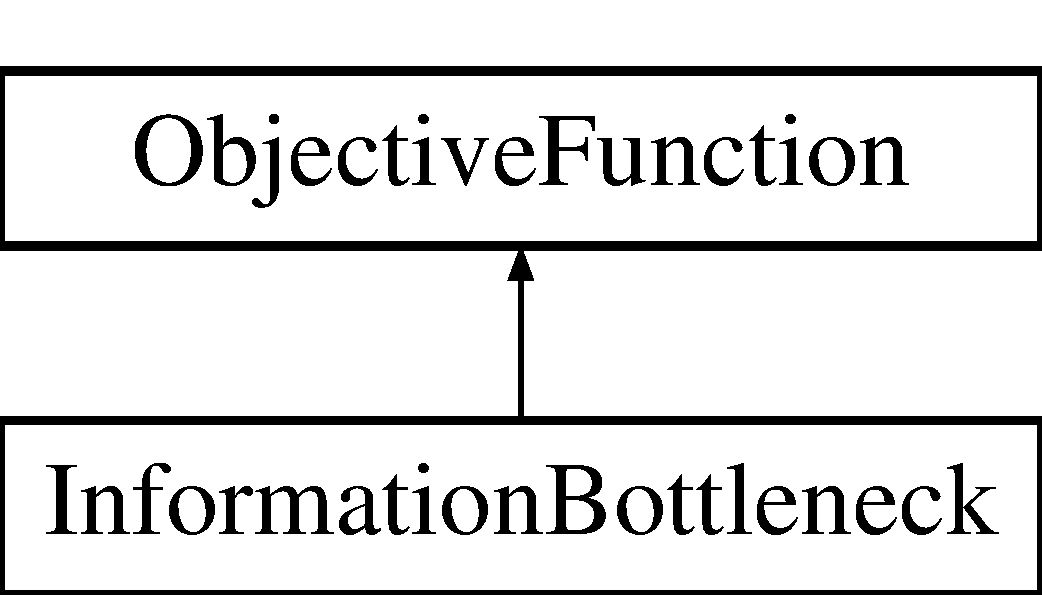
\includegraphics[height=2.000000cm]{classInformationBottleneck}
\end{center}
\end{figure}
\subsection*{Public Member Functions}
\begin{DoxyCompactItemize}
\item 
\hypertarget{classInformationBottleneck_aa2b0adc85665a04330d1356bf77097b6}{{\bfseries Information\-Bottleneck} (\hyperlink{classMarkovProcess}{Markov\-Process} $\ast$process)}\label{classInformationBottleneck_aa2b0adc85665a04330d1356bf77097b6}

\item 
\hypertarget{classInformationBottleneck_a10e4ace575f79977f3f6d2f39403dd84}{void \hyperlink{classInformationBottleneck_a10e4ace575f79977f3f6d2f39403dd84}{set\-Random} ()}\label{classInformationBottleneck_a10e4ace575f79977f3f6d2f39403dd84}

\begin{DoxyCompactList}\small\item\em Randomly set the initial data from which the objective function is computed. \end{DoxyCompactList}\item 
\hypertarget{classInformationBottleneck_af710cb93d1be643a5f67c5d879669b8b}{\hyperlink{classObjectiveValue}{Objective\-Value} $\ast$ \hyperlink{classInformationBottleneck_af710cb93d1be643a5f67c5d879669b8b}{new\-Objective\-Value} (int index=-\/1)}\label{classInformationBottleneck_af710cb93d1be643a5f67c5d879669b8b}

\begin{DoxyCompactList}\small\item\em This method is called by child classes of \hyperlink{classAbstractSet}{Abstract\-Set} (do not use directly) \end{DoxyCompactList}\item 
\hypertarget{classInformationBottleneck_ab3ccf81c8633628cd1a4cc37de61a95b}{double {\bfseries get\-Parameter} (double unit)}\label{classInformationBottleneck_ab3ccf81c8633628cd1a4cc37de61a95b}

\item 
\hypertarget{classInformationBottleneck_a2b29527ef1700808f67ceb1b821a1626}{double {\bfseries get\-Unit\-Distance} (double u\-Min, double u\-Max)}\label{classInformationBottleneck_a2b29527ef1700808f67ceb1b821a1626}

\item 
\hypertarget{classInformationBottleneck_a8a7cc07d65482418e1d62b5f84ec2c45}{double {\bfseries get\-Intermediary\-Unit} (double u\-Min, double u\-Max)}\label{classInformationBottleneck_a8a7cc07d65482418e1d62b5f84ec2c45}

\end{DoxyCompactItemize}
\subsection*{Public Attributes}
\begin{DoxyCompactItemize}
\item 
\hypertarget{classInformationBottleneck_a0d288b82a5d34dff1210d54383ce5997}{\hyperlink{classMarkovProcess}{Markov\-Process} $\ast$ {\bfseries process}}\label{classInformationBottleneck_a0d288b82a5d34dff1210d54383ce5997}

\end{DoxyCompactItemize}


The documentation for this class was generated from the following files\-:\begin{DoxyCompactItemize}
\item 
src/information\-\_\-bottleneck.\-hpp\item 
src/information\-\_\-bottleneck.\-cpp\end{DoxyCompactItemize}

\hypertarget{classLogarithmicObjectiveValue}{\section{Logarithmic\-Objective\-Value Class Reference}
\label{classLogarithmicObjectiveValue}\index{Logarithmic\-Objective\-Value@{Logarithmic\-Objective\-Value}}
}
Inheritance diagram for Logarithmic\-Objective\-Value\-:\begin{figure}[H]
\begin{center}
\leavevmode
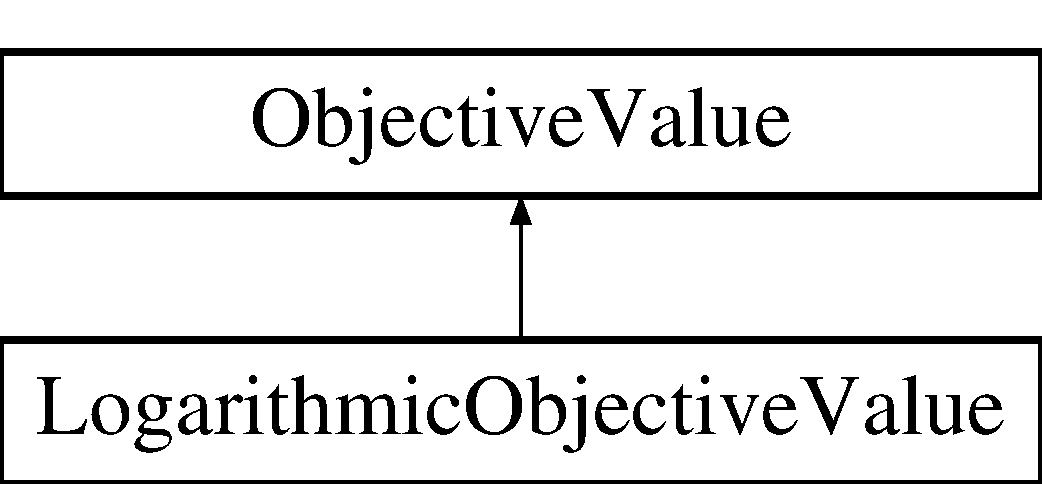
\includegraphics[height=2.000000cm]{classLogarithmicObjectiveValue}
\end{center}
\end{figure}
\subsection*{Public Member Functions}
\begin{DoxyCompactItemize}
\item 
\hypertarget{classLogarithmicObjectiveValue_a5937a9820719eea4339488900bcb1cdb}{{\bfseries Logarithmic\-Objective\-Value} (\hyperlink{classLogarithmicScore}{Logarithmic\-Score} $\ast$objective)}\label{classLogarithmicObjectiveValue_a5937a9820719eea4339488900bcb1cdb}

\item 
\hypertarget{classLogarithmicObjectiveValue_a8b0696f17d27006b70695bdad8174fde}{void {\bfseries add} (\hyperlink{classObjectiveValue}{Objective\-Value} $\ast$value)}\label{classLogarithmicObjectiveValue_a8b0696f17d27006b70695bdad8174fde}

\item 
\hypertarget{classLogarithmicObjectiveValue_a8254a009057b71a9fa2b0aada5a3881c}{void {\bfseries compute} ()}\label{classLogarithmicObjectiveValue_a8254a009057b71a9fa2b0aada5a3881c}

\item 
\hypertarget{classLogarithmicObjectiveValue_a41a261b1cf9ae23bf833e0b6bdb7d555}{void {\bfseries compute} (\hyperlink{classObjectiveValue}{Objective\-Value} $\ast$value1, \hyperlink{classObjectiveValue}{Objective\-Value} $\ast$value2)}\label{classLogarithmicObjectiveValue_a41a261b1cf9ae23bf833e0b6bdb7d555}

\item 
\hypertarget{classLogarithmicObjectiveValue_a39f52d5d09a79e89202b1efe3054d6f3}{void {\bfseries compute} (Objective\-Value\-Set $\ast$valueset)}\label{classLogarithmicObjectiveValue_a39f52d5d09a79e89202b1efe3054d6f3}

\item 
\hypertarget{classLogarithmicObjectiveValue_a86c74627a9ac331a353c74b9a079f35a}{void {\bfseries normalize} (\hyperlink{classObjectiveValue}{Objective\-Value} $\ast$q)}\label{classLogarithmicObjectiveValue_a86c74627a9ac331a353c74b9a079f35a}

\item 
\hypertarget{classLogarithmicObjectiveValue_a0b07eb0a5ec7a61c60395e914aa3ba84}{void {\bfseries print} (bool verbosex=true)}\label{classLogarithmicObjectiveValue_a0b07eb0a5ec7a61c60395e914aa3ba84}

\item 
\hypertarget{classLogarithmicObjectiveValue_a0530e8fb37962ba4a3d9175aac6f6972}{double {\bfseries get\-Value} (double param)}\label{classLogarithmicObjectiveValue_a0530e8fb37962ba4a3d9175aac6f6972}

\end{DoxyCompactItemize}
\subsection*{Public Attributes}
\begin{DoxyCompactItemize}
\item 
\hypertarget{classLogarithmicObjectiveValue_a7b07978deeb0561308efe6bb6a1fd147}{int {\bfseries pre\-Size}}\label{classLogarithmicObjectiveValue_a7b07978deeb0561308efe6bb6a1fd147}

\item 
\hypertarget{classLogarithmicObjectiveValue_aae8e9b82f87468f993b416963fd6c331}{int {\bfseries post\-Size}}\label{classLogarithmicObjectiveValue_aae8e9b82f87468f993b416963fd6c331}

\item 
\hypertarget{classLogarithmicObjectiveValue_a61ff90cabef125963b0da5269c399ee0}{int $\ast$ {\bfseries train\-Count\-Array}}\label{classLogarithmicObjectiveValue_a61ff90cabef125963b0da5269c399ee0}

\item 
\hypertarget{classLogarithmicObjectiveValue_abc923915667f666ce43c9445918d9fa2}{int $\ast$ {\bfseries test\-Count\-Array}}\label{classLogarithmicObjectiveValue_abc923915667f666ce43c9445918d9fa2}

\item 
\hypertarget{classLogarithmicObjectiveValue_ad266163948c5d52072e85f5b0e600881}{int {\bfseries train\-Count\-Total}}\label{classLogarithmicObjectiveValue_ad266163948c5d52072e85f5b0e600881}

\item 
\hypertarget{classLogarithmicObjectiveValue_aa3dcc1ceefeb2e7ba2b547af086ef1a5}{int {\bfseries test\-Count\-Total}}\label{classLogarithmicObjectiveValue_aa3dcc1ceefeb2e7ba2b547af086ef1a5}

\item 
\hypertarget{classLogarithmicObjectiveValue_a1b6e9daa97f490e6da4a06e6dc813ba5}{double {\bfseries score}}\label{classLogarithmicObjectiveValue_a1b6e9daa97f490e6da4a06e6dc813ba5}

\end{DoxyCompactItemize}


The documentation for this class was generated from the following files\-:\begin{DoxyCompactItemize}
\item 
/home/lamarche/programming/optimal\-\_\-partition/src/logarithmic\-\_\-score.\-hpp\item 
/home/lamarche/programming/optimal\-\_\-partition/src/logarithmic\-\_\-score.\-cpp\end{DoxyCompactItemize}

\hypertarget{classLogarithmicScore}{\section{Logarithmic\-Score Class Reference}
\label{classLogarithmicScore}\index{Logarithmic\-Score@{Logarithmic\-Score}}
}


Class to define and compute the logarithmic score function in the case of point prediction.  




{\ttfamily \#include $<$logarithmic\-\_\-score.\-hpp$>$}

Inheritance diagram for Logarithmic\-Score\-:\begin{figure}[H]
\begin{center}
\leavevmode
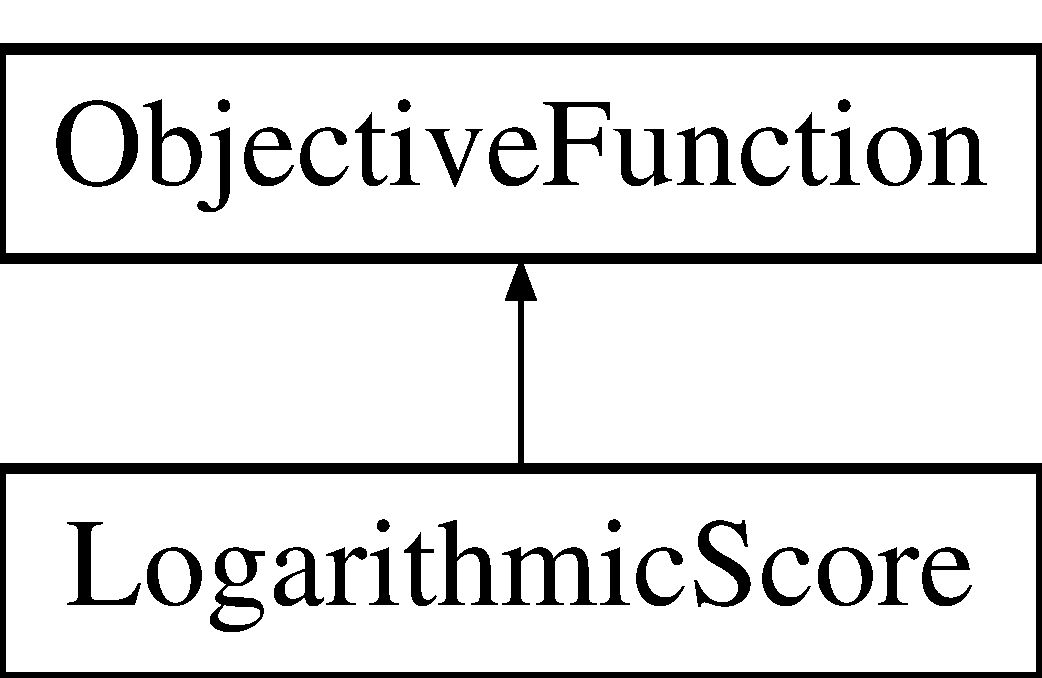
\includegraphics[height=2.000000cm]{classLogarithmicScore}
\end{center}
\end{figure}
\subsection*{Public Member Functions}
\begin{DoxyCompactItemize}
\item 
\hyperlink{classLogarithmicScore_a4fba67dfac53087dbfde7cb825501c97}{Logarithmic\-Score} (\hyperlink{classPredictionDataset}{Prediction\-Dataset} $\ast$dataset, int prior=0)
\begin{DoxyCompactList}\small\item\em Constructor. \end{DoxyCompactList}\item 
\hypertarget{classLogarithmicScore_a08b425a72eec8a2722bb2f4a9b0486ff}{\hyperlink{classLogarithmicScore_a08b425a72eec8a2722bb2f4a9b0486ff}{$\sim$\-Logarithmic\-Score} ()}\label{classLogarithmicScore_a08b425a72eec8a2722bb2f4a9b0486ff}

\begin{DoxyCompactList}\small\item\em Destructor. \end{DoxyCompactList}\item 
\hypertarget{classLogarithmicScore_a7e3c601e96541b3156b02d84ce6b754e}{void \hyperlink{classLogarithmicScore_a7e3c601e96541b3156b02d84ce6b754e}{set\-Random} ()}\label{classLogarithmicScore_a7e3c601e96541b3156b02d84ce6b754e}

\begin{DoxyCompactList}\small\item\em Randomly set the initial data from which the objective function is computed. \end{DoxyCompactList}\item 
\hypertarget{classLogarithmicScore_ab64011283bff491364cdffb0420dc89b}{\hyperlink{classObjectiveValue}{Objective\-Value} $\ast$ \hyperlink{classLogarithmicScore_ab64011283bff491364cdffb0420dc89b}{new\-Objective\-Value} (int index=-\/1)}\label{classLogarithmicScore_ab64011283bff491364cdffb0420dc89b}

\begin{DoxyCompactList}\small\item\em This method is called by child classes of \hyperlink{classAbstractSet}{Abstract\-Set} (do not use directly) \end{DoxyCompactList}\item 
\hypertarget{classLogarithmicScore_ac0a5eb6f03d9afd66a05aded42e6647f}{void \hyperlink{classLogarithmicScore_ac0a5eb6f03d9afd66a05aded42e6647f}{compute\-Objective\-Values} ()}\label{classLogarithmicScore_ac0a5eb6f03d9afd66a05aded42e6647f}

\begin{DoxyCompactList}\small\item\em This method is called by child classes of \hyperlink{classAbstractSet}{Abstract\-Set} (do not use directly) \end{DoxyCompactList}\item 
\hypertarget{classLogarithmicScore_add0be2f6175a2aa0ef5e20026f9eb2be}{void \hyperlink{classLogarithmicScore_add0be2f6175a2aa0ef5e20026f9eb2be}{print\-Objective\-Values} (bool verbose=true)}\label{classLogarithmicScore_add0be2f6175a2aa0ef5e20026f9eb2be}

\begin{DoxyCompactList}\small\item\em This method is called by child classes of \hyperlink{classAbstractSet}{Abstract\-Set} (do not use directly) \end{DoxyCompactList}\item 
\hypertarget{classLogarithmicScore_a33390a7d2b8a14ef7f2e6300a22a4c0b}{double {\bfseries get\-Parameter} (double unit)}\label{classLogarithmicScore_a33390a7d2b8a14ef7f2e6300a22a4c0b}

\item 
\hypertarget{classLogarithmicScore_a123c27f97bfa6071da1f51f39b897bcb}{double {\bfseries get\-Unit\-Distance} (double u\-Min, double u\-Max)}\label{classLogarithmicScore_a123c27f97bfa6071da1f51f39b897bcb}

\item 
\hypertarget{classLogarithmicScore_a40576f47008aa6ab69d95535c0a5fa79}{double {\bfseries get\-Intermediary\-Unit} (double u\-Min, double u\-Max)}\label{classLogarithmicScore_a40576f47008aa6ab69d95535c0a5fa79}

\end{DoxyCompactItemize}
\subsection*{Additional Inherited Members}


\subsection{Detailed Description}
Class to define and compute the logarithmic score function in the case of point prediction. 

\subsection{Constructor \& Destructor Documentation}
\hypertarget{classLogarithmicScore_a4fba67dfac53087dbfde7cb825501c97}{\index{Logarithmic\-Score@{Logarithmic\-Score}!Logarithmic\-Score@{Logarithmic\-Score}}
\index{Logarithmic\-Score@{Logarithmic\-Score}!LogarithmicScore@{Logarithmic\-Score}}
\subsubsection[{Logarithmic\-Score}]{\setlength{\rightskip}{0pt plus 5cm}Logarithmic\-Score\-::\-Logarithmic\-Score (
\begin{DoxyParamCaption}
\item[{{\bf Prediction\-Dataset} $\ast$}]{dataset, }
\item[{int}]{prior = {\ttfamily 0}}
\end{DoxyParamCaption}
)}}\label{classLogarithmicScore_a4fba67dfac53087dbfde7cb825501c97}


Constructor. 


\begin{DoxyParams}{Parameters}
{\em dataset} & \-: The prediction data set that is use to evaluate the score function (from a train set and a test set both containing pre-\/observations and post-\/observations) \\
\hline
{\em prior} & \-: A prior giving the number of times each couple of (pre and post) observations has been observed in addition to the train set \\
\hline
\end{DoxyParams}


The documentation for this class was generated from the following files\-:\begin{DoxyCompactItemize}
\item 
/home/lamarche/programming/optimal\-\_\-partition/src/\hyperlink{logarithmic__score_8hpp}{logarithmic\-\_\-score.\-hpp}\item 
/home/lamarche/programming/optimal\-\_\-partition/src/logarithmic\-\_\-score.\-cpp\end{DoxyCompactItemize}

\hypertarget{classNHONode}{\section{N\-H\-O\-Node Class Reference}
\label{classNHONode}\index{N\-H\-O\-Node@{N\-H\-O\-Node}}
}
\subsection*{Public Member Functions}
\begin{DoxyCompactItemize}
\item 
\hypertarget{classNHONode_a40a898d432184d7e5f23f2a9a75af9b5}{{\bfseries H\-O\-Node} (int size, int index=-\/1)}\label{classNHONode_a40a898d432184d7e5f23f2a9a75af9b5}

\item 
\hypertarget{classNHONode_a680f83500704c65f855241c05f962da6}{int {\bfseries get\-Index} (int i, int j)}\label{classNHONode_a680f83500704c65f855241c05f962da6}

\item 
\hypertarget{classNHONode_a415667d5e0cd35f4a8f9a19da320280f}{void {\bfseries add\-Child} (\hyperlink{classHONode}{H\-O\-Node} $\ast$node)}\label{classNHONode_a415667d5e0cd35f4a8f9a19da320280f}

\item 
\hypertarget{classNHONode_ae5e218f082ae0ae5e0eddae135604a0e}{void {\bfseries set\-Objective\-Function} (\hyperlink{classObjectiveFunction}{Objective\-Function} $\ast$m)}\label{classNHONode_ae5e218f082ae0ae5e0eddae135604a0e}

\item 
\hypertarget{classNHONode_a9bc980f671fcd3574ebabe45d909694b}{void {\bfseries print} ()}\label{classNHONode_a9bc980f671fcd3574ebabe45d909694b}

\item 
\hypertarget{classNHONode_a272cccb7677334ce2b7525ae32d06edb}{void {\bfseries build\-Data\-Structure} (int level=0)}\label{classNHONode_a272cccb7677334ce2b7525ae32d06edb}

\item 
\hypertarget{classNHONode_a0c6c281eb16a3525ca1c0046abb53c8a}{void {\bfseries compute\-Objective\-Values} ()}\label{classNHONode_a0c6c281eb16a3525ca1c0046abb53c8a}

\item 
\hypertarget{classNHONode_af3ff05d5429f657e1e8fe881f88e711b}{void {\bfseries normalize\-Objective\-Values} (\hyperlink{classObjectiveValue}{Objective\-Value} $\ast$max\-Qual=0)}\label{classNHONode_af3ff05d5429f657e1e8fe881f88e711b}

\item 
\hypertarget{classNHONode_a615ee571b738b3fe0d60e0ed1acc7612}{void {\bfseries print\-Objective\-Values} ()}\label{classNHONode_a615ee571b738b3fe0d60e0ed1acc7612}

\item 
\hypertarget{classNHONode_a4cab45b2ba487bb6573fcd91d1495d05}{void {\bfseries compute\-Optimal\-Partition} (double parameter)}\label{classNHONode_a4cab45b2ba487bb6573fcd91d1495d05}

\item 
\hypertarget{classNHONode_a49eda2179eb77aa824e4a853a5576621}{void {\bfseries print\-Optimal\-Partition} (double parameter)}\label{classNHONode_a49eda2179eb77aa824e4a853a5576621}

\item 
\hypertarget{classNHONode_ab31e6785db37a35332bfc538b873bb44}{\hyperlink{classPartition}{Partition} $\ast$ {\bfseries get\-Optimal\-Partition} (double parameter)}\label{classNHONode_ab31e6785db37a35332bfc538b873bb44}

\item 
\hypertarget{classNHONode_a67d75346ed592f669f0029c2e1550371}{void {\bfseries build\-Optimal\-Partition} (\hyperlink{classPartition}{Partition} $\ast$partition, int pi=0, int pj=-\/1)}\label{classNHONode_a67d75346ed592f669f0029c2e1550371}

\end{DoxyCompactItemize}
\subsection*{Public Attributes}
\begin{DoxyCompactItemize}
\item 
\hypertarget{classNHONode_a013a329d2040bad27a73441713cc6889}{int {\bfseries index}}\label{classNHONode_a013a329d2040bad27a73441713cc6889}

\item 
\hypertarget{classNHONode_ac8986878a95cff24e48213bb5797f16b}{int {\bfseries level}}\label{classNHONode_ac8986878a95cff24e48213bb5797f16b}

\item 
\hypertarget{classNHONode_a0aa84b08ee2451dce8e3cdf4326eb8f4}{std\-::set$<$ int $>$ $\ast$ {\bfseries indices}}\label{classNHONode_a0aa84b08ee2451dce8e3cdf4326eb8f4}

\item 
\hypertarget{classNHONode_a0ba248697389f672625383d1f3ad1b1c}{H\-O\-Node\-Set $\ast$ {\bfseries children}}\label{classNHONode_a0ba248697389f672625383d1f3ad1b1c}

\item 
\hypertarget{classNHONode_acab2ed08c3d77ece7104c30359d2aa58}{\hyperlink{classObjectiveFunction}{Objective\-Function} $\ast$ {\bfseries objective}}\label{classNHONode_acab2ed08c3d77ece7104c30359d2aa58}

\item 
\hypertarget{classNHONode_a0df5a9dd324f86be0164a54fe80cf5b0}{int {\bfseries size}}\label{classNHONode_a0df5a9dd324f86be0164a54fe80cf5b0}

\item 
\hypertarget{classNHONode_a40c3a14d897eff575063ba8e99449279}{\hyperlink{classObjectiveValue}{Objective\-Value} $\ast$$\ast$ {\bfseries qualities}}\label{classNHONode_a40c3a14d897eff575063ba8e99449279}

\item 
\hypertarget{classNHONode_a4e5234e92269a9bdb391c0e4d2f7f83e}{double $\ast$ {\bfseries optimal\-Values}}\label{classNHONode_a4e5234e92269a9bdb391c0e4d2f7f83e}

\item 
\hypertarget{classNHONode_ab98175d354eac8ecfe571ec7ae6919d4}{int $\ast$ {\bfseries optimal\-Cuts}}\label{classNHONode_ab98175d354eac8ecfe571ec7ae6919d4}

\end{DoxyCompactItemize}


The documentation for this class was generated from the following file\-:\begin{DoxyCompactItemize}
\item 
/home/lamarche/programming/optimal\-\_\-partition/src/N\-H\-O\-\_\-set.\-hpp\end{DoxyCompactItemize}

\hypertarget{classNHOSet}{\section{N\-H\-O\-Set Class Reference}
\label{classNHOSet}\index{N\-H\-O\-Set@{N\-H\-O\-Set}}
}
Inheritance diagram for N\-H\-O\-Set\-:\begin{figure}[H]
\begin{center}
\leavevmode
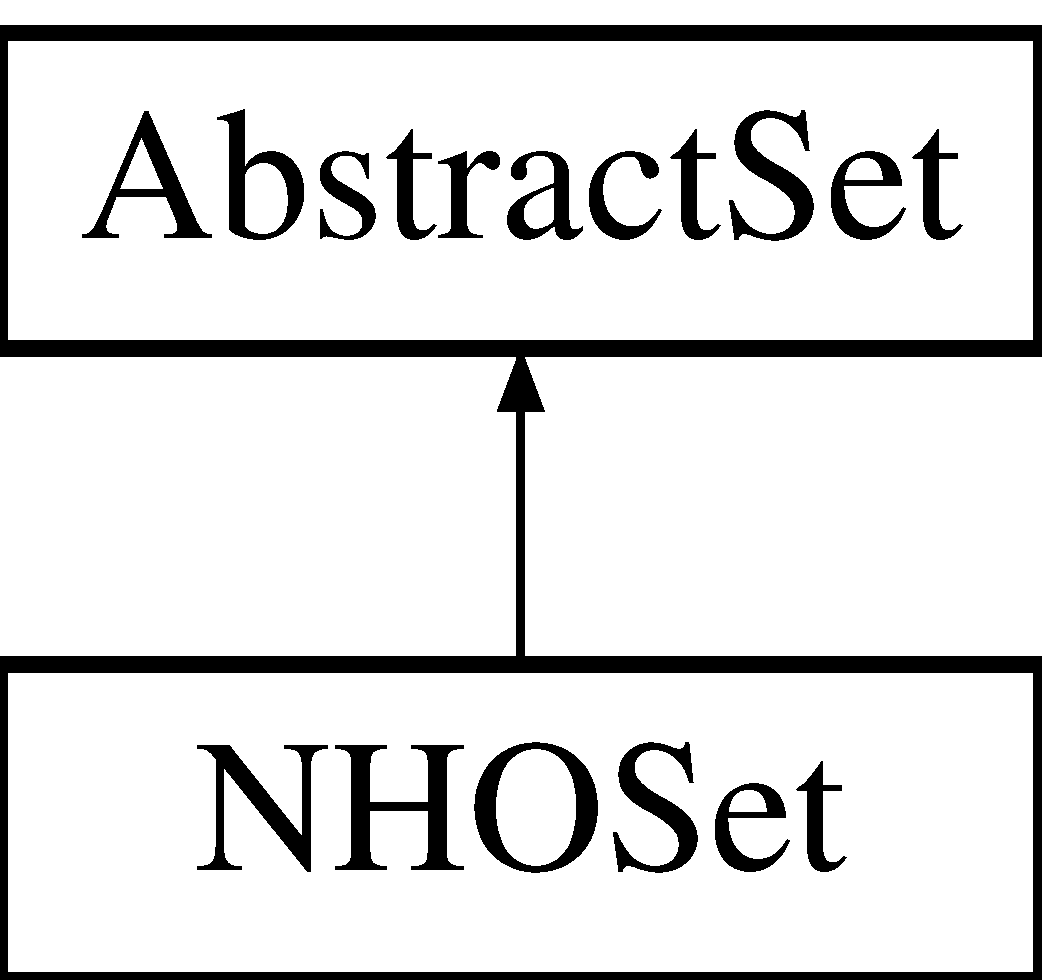
\includegraphics[height=2.000000cm]{classNHOSet}
\end{center}
\end{figure}
\subsection*{Public Member Functions}
\begin{DoxyCompactItemize}
\item 
\hypertarget{classNHOSet_a742973945209773c1e9011f8637fe05b}{{\bfseries N\-H\-O\-Set} (int N\-Size, \hyperlink{classHNode}{H\-Node} $\ast$H\-Hierarchy, int O\-Size)}\label{classNHOSet_a742973945209773c1e9011f8637fe05b}

\item 
\hypertarget{classNHOSet_ae73a4b22551df422392087730c9c26fd}{void \hyperlink{classNHOSet_ae73a4b22551df422392087730c9c26fd}{set\-Random} ()}\label{classNHOSet_ae73a4b22551df422392087730c9c26fd}

\begin{DoxyCompactList}\small\item\em Randomly set the algebraic constraints for quick experiments (warning\-: this method is not always implemented) \end{DoxyCompactList}\item 
void \hyperlink{classNHOSet_ac1e59897d3af9dd6c019d6db9bb74dd1}{set\-Objective\-Function} (\hyperlink{classObjectiveFunction}{Objective\-Function} $\ast$m)
\begin{DoxyCompactList}\small\item\em Set the objective that one wants to optimise. \end{DoxyCompactList}\item 
\hypertarget{classNHOSet_ad4e76f5034d84cb5c43c6df373113187}{void \hyperlink{classNHOSet_ad4e76f5034d84cb5c43c6df373113187}{print} ()}\label{classNHOSet_ad4e76f5034d84cb5c43c6df373113187}

\begin{DoxyCompactList}\small\item\em Print the set and its algebraic constraints. \end{DoxyCompactList}\item 
\hypertarget{classNHOSet_a97466bc5172f0e509f6a311a57b2e68c}{void \hyperlink{classNHOSet_a97466bc5172f0e509f6a311a57b2e68c}{build\-Data\-Structure} ()}\label{classNHOSet_a97466bc5172f0e509f6a311a57b2e68c}

\begin{DoxyCompactList}\small\item\em Build a proper data structure to represent the set and its algebraic constraints (warning\-: this method should always be called after instantiating and parameterising a set, and before calling any other method, such as \hyperlink{classNHOSet_ad4e76f5034d84cb5c43c6df373113187}{print()}, \hyperlink{classNHOSet_a8f1438a5867b733f2788536609fbe18f}{compute\-Objective\-Values()}, compute\-Optimal\-Partition (double parameter), etc.) \end{DoxyCompactList}\item 
\hypertarget{classNHOSet_a8f1438a5867b733f2788536609fbe18f}{void \hyperlink{classNHOSet_a8f1438a5867b733f2788536609fbe18f}{compute\-Objective\-Values} ()}\label{classNHOSet_a8f1438a5867b733f2788536609fbe18f}

\begin{DoxyCompactList}\small\item\em Compute the value of the objective function for each feasible part (warning\-: set\-Objective\-Function (\hyperlink{classObjectiveFunction}{Objective\-Function} $\ast$objective) should have been called first) \end{DoxyCompactList}\item 
\hypertarget{classNHOSet_a19a2fa37a137eb7ff2459c5c6a0f9eb4}{void \hyperlink{classNHOSet_a19a2fa37a137eb7ff2459c5c6a0f9eb4}{normalize\-Objective\-Values} ()}\label{classNHOSet_a19a2fa37a137eb7ff2459c5c6a0f9eb4}

\begin{DoxyCompactList}\small\item\em Finish computing the value of the objective function for each feasible part when normalisation is required (warning\-: only after \hyperlink{classNHOSet_a8f1438a5867b733f2788536609fbe18f}{compute\-Objective\-Values()} has been called) \end{DoxyCompactList}\item 
\hypertarget{classNHOSet_af84d4b1f3b7c0adedbd7561545b8b2f0}{void \hyperlink{classNHOSet_af84d4b1f3b7c0adedbd7561545b8b2f0}{print\-Objective\-Values} ()}\label{classNHOSet_af84d4b1f3b7c0adedbd7561545b8b2f0}

\begin{DoxyCompactList}\small\item\em Print the value of the objective function for each feasible part. \end{DoxyCompactList}\item 
void \hyperlink{classNHOSet_ae3d2e2f17d62402efbf0564e8b10ec1c}{compute\-Optimal\-Partition} (double parameter)
\begin{DoxyCompactList}\small\item\em Compute a partition that fits with the algebraic constraints and that optimises the objective function that has been specified. \end{DoxyCompactList}\item 
void \hyperlink{classNHOSet_ad30bf8268a25aca0f11115e526ef7536}{print\-Optimal\-Partition} (double parameter)
\begin{DoxyCompactList}\small\item\em Compute and print a partition that fits with the algebraic constraints and that optimises the objective function that has been specified (warning\-: this method is not always implemented, but one can obtain a similar result by using get\-Optimal\-Partition (double parameter) and by calling \hyperlink{classNHOSet_ad4e76f5034d84cb5c43c6df373113187}{print()} on the result) \end{DoxyCompactList}\item 
\hyperlink{classPartition}{Partition} $\ast$ \hyperlink{classNHOSet_a2269a3b8f493512859660d3a457303d7}{get\-Optimal\-Partition} (double parameter)
\begin{DoxyCompactList}\small\item\em Compute and return a partition that fits with the algebraic constraints and that optimises the objective function that has been specified (warning\-: this method is not always implemented, but one can obtain a similar result by using get\-Optimal\-Partition (double parameter) and by calling \hyperlink{classNHOSet_ad4e76f5034d84cb5c43c6df373113187}{print()} on the result) \end{DoxyCompactList}\end{DoxyCompactItemize}
\subsection*{Public Attributes}
\begin{DoxyCompactItemize}
\item 
\hypertarget{classNHOSet_a0f67bd55ed5a178196c783f827dc75e6}{int {\bfseries N\-Size}}\label{classNHOSet_a0f67bd55ed5a178196c783f827dc75e6}

\item 
\hypertarget{classNHOSet_a4f27b2f8a1f743f3e0e66b2a8c7299cc}{\hyperlink{classHNode}{H\-Node} $\ast$ {\bfseries H\-Hierarchy}}\label{classNHOSet_a4f27b2f8a1f743f3e0e66b2a8c7299cc}

\item 
\hypertarget{classNHOSet_aafdd06ce3ed3a043b97f846b36115a36}{int {\bfseries O\-Size}}\label{classNHOSet_aafdd06ce3ed3a043b97f846b36115a36}

\item 
\hypertarget{classNHOSet_a083e3975e9efd5710770068145eae84a}{N\-H\-O\-Datatree $\ast$ {\bfseries N\-H\-O\-Datatree}}\label{classNHOSet_a083e3975e9efd5710770068145eae84a}

\end{DoxyCompactItemize}


\subsection{Member Function Documentation}
\hypertarget{classNHOSet_ae3d2e2f17d62402efbf0564e8b10ec1c}{\index{N\-H\-O\-Set@{N\-H\-O\-Set}!compute\-Optimal\-Partition@{compute\-Optimal\-Partition}}
\index{compute\-Optimal\-Partition@{compute\-Optimal\-Partition}!NHOSet@{N\-H\-O\-Set}}
\subsubsection[{compute\-Optimal\-Partition}]{\setlength{\rightskip}{0pt plus 5cm}void N\-H\-O\-Set\-::compute\-Optimal\-Partition (
\begin{DoxyParamCaption}
\item[{double}]{parameter}
\end{DoxyParamCaption}
)\hspace{0.3cm}{\ttfamily [virtual]}}}\label{classNHOSet_ae3d2e2f17d62402efbf0564e8b10ec1c}


Compute a partition that fits with the algebraic constraints and that optimises the objective function that has been specified. 


\begin{DoxyParams}{Parameters}
{\em parameter} & \-: The parameter of the objective function to be optimised (if the objective is parametrised) \\
\hline
\end{DoxyParams}


Implements \hyperlink{classAbstractSet_acfc3004f18192f38e32bb7a5a12ec8df}{Abstract\-Set}.

\hypertarget{classNHOSet_a2269a3b8f493512859660d3a457303d7}{\index{N\-H\-O\-Set@{N\-H\-O\-Set}!get\-Optimal\-Partition@{get\-Optimal\-Partition}}
\index{get\-Optimal\-Partition@{get\-Optimal\-Partition}!NHOSet@{N\-H\-O\-Set}}
\subsubsection[{get\-Optimal\-Partition}]{\setlength{\rightskip}{0pt plus 5cm}{\bf Partition}$\ast$ N\-H\-O\-Set\-::get\-Optimal\-Partition (
\begin{DoxyParamCaption}
\item[{double}]{parameter}
\end{DoxyParamCaption}
)\hspace{0.3cm}{\ttfamily [virtual]}}}\label{classNHOSet_a2269a3b8f493512859660d3a457303d7}


Compute and return a partition that fits with the algebraic constraints and that optimises the objective function that has been specified (warning\-: this method is not always implemented, but one can obtain a similar result by using get\-Optimal\-Partition (double parameter) and by calling \hyperlink{classNHOSet_ad4e76f5034d84cb5c43c6df373113187}{print()} on the result) 


\begin{DoxyParams}{Parameters}
{\em parameter} & \-: The parameter of the objective function to be optimised (if the objective is parametrised) \\
\hline
\end{DoxyParams}
\begin{DoxyReturn}{Returns}
\-: The resulting optimal partition 
\end{DoxyReturn}


Implements \hyperlink{classAbstractSet_a48fd08c4b61ed46946bed6e19cd11194}{Abstract\-Set}.

\hypertarget{classNHOSet_ad30bf8268a25aca0f11115e526ef7536}{\index{N\-H\-O\-Set@{N\-H\-O\-Set}!print\-Optimal\-Partition@{print\-Optimal\-Partition}}
\index{print\-Optimal\-Partition@{print\-Optimal\-Partition}!NHOSet@{N\-H\-O\-Set}}
\subsubsection[{print\-Optimal\-Partition}]{\setlength{\rightskip}{0pt plus 5cm}void N\-H\-O\-Set\-::print\-Optimal\-Partition (
\begin{DoxyParamCaption}
\item[{double}]{parameter}
\end{DoxyParamCaption}
)\hspace{0.3cm}{\ttfamily [virtual]}}}\label{classNHOSet_ad30bf8268a25aca0f11115e526ef7536}


Compute and print a partition that fits with the algebraic constraints and that optimises the objective function that has been specified (warning\-: this method is not always implemented, but one can obtain a similar result by using get\-Optimal\-Partition (double parameter) and by calling \hyperlink{classNHOSet_ad4e76f5034d84cb5c43c6df373113187}{print()} on the result) 


\begin{DoxyParams}{Parameters}
{\em parameter} & \-: The parameter of the objective function to be optimised (if the objective is parametrised) \\
\hline
\end{DoxyParams}


Implements \hyperlink{classAbstractSet_a82a9ce5c2d30690f0d1b83b034e92e1e}{Abstract\-Set}.

\hypertarget{classNHOSet_ac1e59897d3af9dd6c019d6db9bb74dd1}{\index{N\-H\-O\-Set@{N\-H\-O\-Set}!set\-Objective\-Function@{set\-Objective\-Function}}
\index{set\-Objective\-Function@{set\-Objective\-Function}!NHOSet@{N\-H\-O\-Set}}
\subsubsection[{set\-Objective\-Function}]{\setlength{\rightskip}{0pt plus 5cm}void N\-H\-O\-Set\-::set\-Objective\-Function (
\begin{DoxyParamCaption}
\item[{{\bf Objective\-Function} $\ast$}]{objective}
\end{DoxyParamCaption}
)\hspace{0.3cm}{\ttfamily [virtual]}}}\label{classNHOSet_ac1e59897d3af9dd6c019d6db9bb74dd1}


Set the objective that one wants to optimise. 


\begin{DoxyParams}{Parameters}
{\em objective} & \-: The objective function itself \\
\hline
\end{DoxyParams}


Implements \hyperlink{classAbstractSet_a7aef71679a18ab7965d1098da15b26c2}{Abstract\-Set}.



The documentation for this class was generated from the following file\-:\begin{DoxyCompactItemize}
\item 
/home/lamarche/programming/optimal\-\_\-partition/src/N\-H\-O\-\_\-set.\-hpp\end{DoxyCompactItemize}

\hypertarget{classNonconstrainedOrderedSet}{\section{Nonconstrained\-Ordered\-Set Class Reference}
\label{classNonconstrainedOrderedSet}\index{Nonconstrained\-Ordered\-Set@{Nonconstrained\-Ordered\-Set}}
}
Inheritance diagram for Nonconstrained\-Ordered\-Set\-:\begin{figure}[H]
\begin{center}
\leavevmode
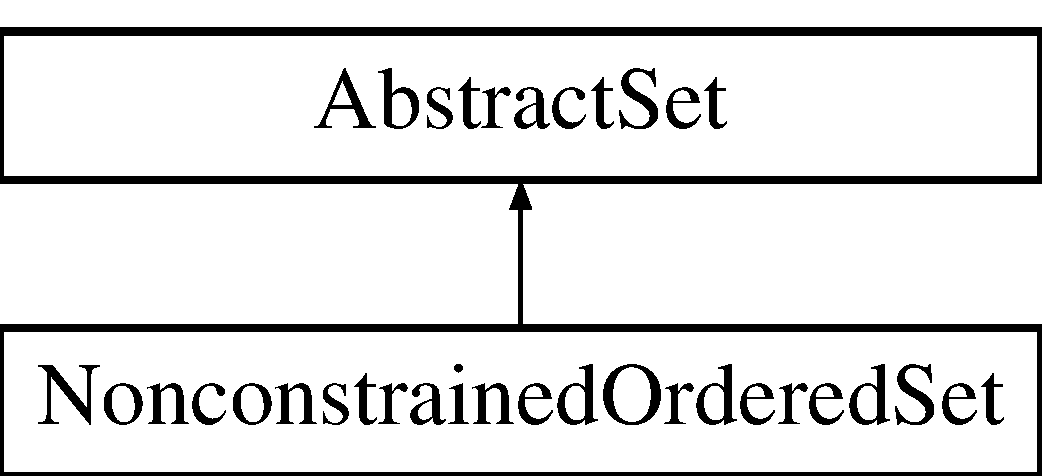
\includegraphics[height=2.000000cm]{classNonconstrainedOrderedSet}
\end{center}
\end{figure}
\subsection*{Public Member Functions}
\begin{DoxyCompactItemize}
\item 
\hypertarget{classNonconstrainedOrderedSet_a6651cd5e2b0993f58ec8b60adf98593d}{{\bfseries Nonconstrained\-Ordered\-Set} (int size1, int size2)}\label{classNonconstrainedOrderedSet_a6651cd5e2b0993f58ec8b60adf98593d}

\item 
\hypertarget{classNonconstrainedOrderedSet_a731b472b246c259509c6bc0175972aca}{void \hyperlink{classNonconstrainedOrderedSet_a731b472b246c259509c6bc0175972aca}{set\-Random} ()}\label{classNonconstrainedOrderedSet_a731b472b246c259509c6bc0175972aca}

\begin{DoxyCompactList}\small\item\em Randomly set the algebraic constraints for quick experiments (warning\-: this method is not always implemented) \end{DoxyCompactList}\item 
void \hyperlink{classNonconstrainedOrderedSet_a67a4a72a5e1bff3d46473757199455d9}{set\-Objective\-Function} (\hyperlink{classObjectiveFunction}{Objective\-Function} $\ast$m)
\begin{DoxyCompactList}\small\item\em Set the objective that one wants to optimise. \end{DoxyCompactList}\item 
\hypertarget{classNonconstrainedOrderedSet_a19a923ee00c1ea0bbf875b2166099b0e}{void \hyperlink{classNonconstrainedOrderedSet_a19a923ee00c1ea0bbf875b2166099b0e}{print} ()}\label{classNonconstrainedOrderedSet_a19a923ee00c1ea0bbf875b2166099b0e}

\begin{DoxyCompactList}\small\item\em Print the set and its algebraic constraints. \end{DoxyCompactList}\item 
\hypertarget{classNonconstrainedOrderedSet_a53251872f1e632d770c971ca74552533}{void \hyperlink{classNonconstrainedOrderedSet_a53251872f1e632d770c971ca74552533}{build\-Data\-Structure} ()}\label{classNonconstrainedOrderedSet_a53251872f1e632d770c971ca74552533}

\begin{DoxyCompactList}\small\item\em Build a proper data structure to represent the set and its algebraic constraints (warning\-: this method should always be called after instantiating and parameterising a set, and before calling any other method, such as \hyperlink{classNonconstrainedOrderedSet_a19a923ee00c1ea0bbf875b2166099b0e}{print()}, \hyperlink{classNonconstrainedOrderedSet_a26d8952d918cbd549ae66d0e595c1b44}{compute\-Objective\-Values()}, compute\-Optimal\-Partition (double parameter), etc.) \end{DoxyCompactList}\item 
\hypertarget{classNonconstrainedOrderedSet_a26d8952d918cbd549ae66d0e595c1b44}{void \hyperlink{classNonconstrainedOrderedSet_a26d8952d918cbd549ae66d0e595c1b44}{compute\-Objective\-Values} ()}\label{classNonconstrainedOrderedSet_a26d8952d918cbd549ae66d0e595c1b44}

\begin{DoxyCompactList}\small\item\em Compute the value of the objective function for each feasible part (warning\-: set\-Objective\-Function (\hyperlink{classObjectiveFunction}{Objective\-Function} $\ast$objective) should have been called first) \end{DoxyCompactList}\item 
\hypertarget{classNonconstrainedOrderedSet_acf86c9802cb55ff5d41379b9de4f2b6b}{void \hyperlink{classNonconstrainedOrderedSet_acf86c9802cb55ff5d41379b9de4f2b6b}{normalize\-Objective\-Values} ()}\label{classNonconstrainedOrderedSet_acf86c9802cb55ff5d41379b9de4f2b6b}

\begin{DoxyCompactList}\small\item\em Finish computing the value of the objective function for each feasible part when normalisation is required (warning\-: only after \hyperlink{classNonconstrainedOrderedSet_a26d8952d918cbd549ae66d0e595c1b44}{compute\-Objective\-Values()} has been called) \end{DoxyCompactList}\item 
\hypertarget{classNonconstrainedOrderedSet_a23614dac2b35a8139612b48c25beb2d1}{void \hyperlink{classNonconstrainedOrderedSet_a23614dac2b35a8139612b48c25beb2d1}{print\-Objective\-Values} ()}\label{classNonconstrainedOrderedSet_a23614dac2b35a8139612b48c25beb2d1}

\begin{DoxyCompactList}\small\item\em Print the value of the objective function for each feasible part. \end{DoxyCompactList}\item 
void \hyperlink{classNonconstrainedOrderedSet_a1a880ae970c47446a370a4b4679b59f5}{compute\-Optimal\-Partition} (double parameter)
\begin{DoxyCompactList}\small\item\em Compute a partition that fits with the algebraic constraints and that optimises the objective function that has been specified. \end{DoxyCompactList}\item 
void \hyperlink{classNonconstrainedOrderedSet_a2fe53fd392a2b76a994b47857e8b9f8d}{print\-Optimal\-Partition} (double parameter)
\begin{DoxyCompactList}\small\item\em Compute and print a partition that fits with the algebraic constraints and that optimises the objective function that has been specified (warning\-: this method is not always implemented, but one can obtain a similar result by using get\-Optimal\-Partition (double parameter) and by calling \hyperlink{classNonconstrainedOrderedSet_a19a923ee00c1ea0bbf875b2166099b0e}{print()} on the result) \end{DoxyCompactList}\item 
\hyperlink{classPartition}{Partition} $\ast$ \hyperlink{classNonconstrainedOrderedSet_a56bc624037070551d43a72685bbe2347}{get\-Optimal\-Partition} (double parameter)
\begin{DoxyCompactList}\small\item\em Compute and return a partition that fits with the algebraic constraints and that optimises the objective function that has been specified (warning\-: this method is not always implemented, but one can obtain a similar result by using get\-Optimal\-Partition (double parameter) and by calling \hyperlink{classNonconstrainedOrderedSet_a19a923ee00c1ea0bbf875b2166099b0e}{print()} on the result) \end{DoxyCompactList}\end{DoxyCompactItemize}
\subsection*{Public Attributes}
\begin{DoxyCompactItemize}
\item 
\hypertarget{classNonconstrainedOrderedSet_a288742a1e94bd5059885a615c53fda3f}{int {\bfseries size1}}\label{classNonconstrainedOrderedSet_a288742a1e94bd5059885a615c53fda3f}

\item 
\hypertarget{classNonconstrainedOrderedSet_acef74e3fc45f4f07398076cdca8a4184}{int {\bfseries size2}}\label{classNonconstrainedOrderedSet_acef74e3fc45f4f07398076cdca8a4184}

\item 
\hypertarget{classNonconstrainedOrderedSet_a9ff9bbb398682cce7e3d6cd5bf39ebc7}{\hyperlink{classOrderedDatatree}{Ordered\-Datatree} $\ast$ {\bfseries data\-Tree}}\label{classNonconstrainedOrderedSet_a9ff9bbb398682cce7e3d6cd5bf39ebc7}

\item 
\hypertarget{classNonconstrainedOrderedSet_a7ee6387a6e18c48828b2349e3b8a3533}{\hyperlink{classObjectiveValue}{Objective\-Value} $\ast$$\ast$ {\bfseries qualities}}\label{classNonconstrainedOrderedSet_a7ee6387a6e18c48828b2349e3b8a3533}

\end{DoxyCompactItemize}


\subsection{Member Function Documentation}
\hypertarget{classNonconstrainedOrderedSet_a1a880ae970c47446a370a4b4679b59f5}{\index{Nonconstrained\-Ordered\-Set@{Nonconstrained\-Ordered\-Set}!compute\-Optimal\-Partition@{compute\-Optimal\-Partition}}
\index{compute\-Optimal\-Partition@{compute\-Optimal\-Partition}!NonconstrainedOrderedSet@{Nonconstrained\-Ordered\-Set}}
\subsubsection[{compute\-Optimal\-Partition}]{\setlength{\rightskip}{0pt plus 5cm}void Nonconstrained\-Ordered\-Set\-::compute\-Optimal\-Partition (
\begin{DoxyParamCaption}
\item[{double}]{parameter}
\end{DoxyParamCaption}
)\hspace{0.3cm}{\ttfamily [virtual]}}}\label{classNonconstrainedOrderedSet_a1a880ae970c47446a370a4b4679b59f5}


Compute a partition that fits with the algebraic constraints and that optimises the objective function that has been specified. 


\begin{DoxyParams}{Parameters}
{\em parameter} & \-: The parameter of the objective function to be optimised (if the objective is parametrised) \\
\hline
\end{DoxyParams}


Implements \hyperlink{classAbstractSet_acfc3004f18192f38e32bb7a5a12ec8df}{Abstract\-Set}.

\hypertarget{classNonconstrainedOrderedSet_a56bc624037070551d43a72685bbe2347}{\index{Nonconstrained\-Ordered\-Set@{Nonconstrained\-Ordered\-Set}!get\-Optimal\-Partition@{get\-Optimal\-Partition}}
\index{get\-Optimal\-Partition@{get\-Optimal\-Partition}!NonconstrainedOrderedSet@{Nonconstrained\-Ordered\-Set}}
\subsubsection[{get\-Optimal\-Partition}]{\setlength{\rightskip}{0pt plus 5cm}{\bf Partition} $\ast$ Nonconstrained\-Ordered\-Set\-::get\-Optimal\-Partition (
\begin{DoxyParamCaption}
\item[{double}]{parameter}
\end{DoxyParamCaption}
)\hspace{0.3cm}{\ttfamily [virtual]}}}\label{classNonconstrainedOrderedSet_a56bc624037070551d43a72685bbe2347}


Compute and return a partition that fits with the algebraic constraints and that optimises the objective function that has been specified (warning\-: this method is not always implemented, but one can obtain a similar result by using get\-Optimal\-Partition (double parameter) and by calling \hyperlink{classNonconstrainedOrderedSet_a19a923ee00c1ea0bbf875b2166099b0e}{print()} on the result) 


\begin{DoxyParams}{Parameters}
{\em parameter} & \-: The parameter of the objective function to be optimised (if the objective is parametrised) \\
\hline
\end{DoxyParams}
\begin{DoxyReturn}{Returns}
\-: The resulting optimal partition 
\end{DoxyReturn}


Implements \hyperlink{classAbstractSet_a48fd08c4b61ed46946bed6e19cd11194}{Abstract\-Set}.

\hypertarget{classNonconstrainedOrderedSet_a2fe53fd392a2b76a994b47857e8b9f8d}{\index{Nonconstrained\-Ordered\-Set@{Nonconstrained\-Ordered\-Set}!print\-Optimal\-Partition@{print\-Optimal\-Partition}}
\index{print\-Optimal\-Partition@{print\-Optimal\-Partition}!NonconstrainedOrderedSet@{Nonconstrained\-Ordered\-Set}}
\subsubsection[{print\-Optimal\-Partition}]{\setlength{\rightskip}{0pt plus 5cm}void Nonconstrained\-Ordered\-Set\-::print\-Optimal\-Partition (
\begin{DoxyParamCaption}
\item[{double}]{parameter}
\end{DoxyParamCaption}
)\hspace{0.3cm}{\ttfamily [virtual]}}}\label{classNonconstrainedOrderedSet_a2fe53fd392a2b76a994b47857e8b9f8d}


Compute and print a partition that fits with the algebraic constraints and that optimises the objective function that has been specified (warning\-: this method is not always implemented, but one can obtain a similar result by using get\-Optimal\-Partition (double parameter) and by calling \hyperlink{classNonconstrainedOrderedSet_a19a923ee00c1ea0bbf875b2166099b0e}{print()} on the result) 


\begin{DoxyParams}{Parameters}
{\em parameter} & \-: The parameter of the objective function to be optimised (if the objective is parametrised) \\
\hline
\end{DoxyParams}


Implements \hyperlink{classAbstractSet_a82a9ce5c2d30690f0d1b83b034e92e1e}{Abstract\-Set}.

\hypertarget{classNonconstrainedOrderedSet_a67a4a72a5e1bff3d46473757199455d9}{\index{Nonconstrained\-Ordered\-Set@{Nonconstrained\-Ordered\-Set}!set\-Objective\-Function@{set\-Objective\-Function}}
\index{set\-Objective\-Function@{set\-Objective\-Function}!NonconstrainedOrderedSet@{Nonconstrained\-Ordered\-Set}}
\subsubsection[{set\-Objective\-Function}]{\setlength{\rightskip}{0pt plus 5cm}void Nonconstrained\-Ordered\-Set\-::set\-Objective\-Function (
\begin{DoxyParamCaption}
\item[{{\bf Objective\-Function} $\ast$}]{objective}
\end{DoxyParamCaption}
)\hspace{0.3cm}{\ttfamily [virtual]}}}\label{classNonconstrainedOrderedSet_a67a4a72a5e1bff3d46473757199455d9}


Set the objective that one wants to optimise. 


\begin{DoxyParams}{Parameters}
{\em objective} & \-: The objective function itself \\
\hline
\end{DoxyParams}


Implements \hyperlink{classAbstractSet_a7aef71679a18ab7965d1098da15b26c2}{Abstract\-Set}.



The documentation for this class was generated from the following files\-:\begin{DoxyCompactItemize}
\item 
src/nonconstrained\-\_\-ordered\-\_\-set.\-hpp\item 
src/nonconstrained\-\_\-ordered\-\_\-set.\-cpp\end{DoxyCompactItemize}

\hypertarget{classNonconstrainedSet}{\section{Nonconstrained\-Set Class Reference}
\label{classNonconstrainedSet}\index{Nonconstrained\-Set@{Nonconstrained\-Set}}
}
Inheritance diagram for Nonconstrained\-Set\-:\begin{figure}[H]
\begin{center}
\leavevmode
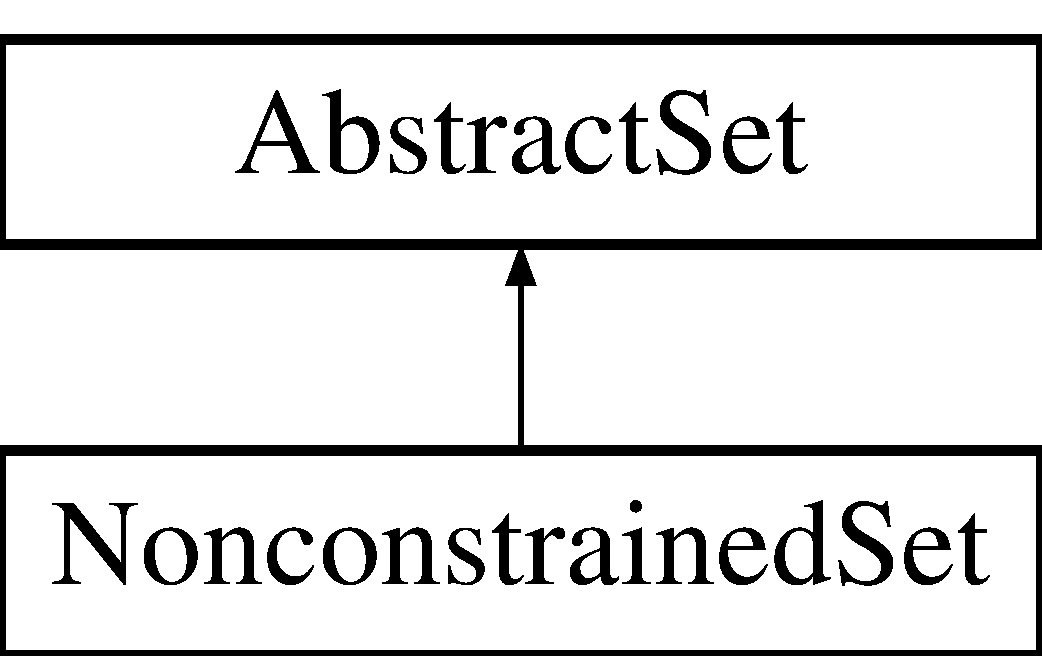
\includegraphics[height=2.000000cm]{classNonconstrainedSet}
\end{center}
\end{figure}
\subsection*{Public Member Functions}
\begin{DoxyCompactItemize}
\item 
\hypertarget{classNonconstrainedSet_a796dd2d6fdf3df03c3b1c3ddacd3c97b}{{\bfseries Nonconstrained\-Set} (int size)}\label{classNonconstrainedSet_a796dd2d6fdf3df03c3b1c3ddacd3c97b}

\item 
\hypertarget{classNonconstrainedSet_a71c6b8dfd1b2abbed3c712464c6c2538}{void \hyperlink{classNonconstrainedSet_a71c6b8dfd1b2abbed3c712464c6c2538}{set\-Random} ()}\label{classNonconstrainedSet_a71c6b8dfd1b2abbed3c712464c6c2538}

\begin{DoxyCompactList}\small\item\em Randomly set the algebraic constraints for quick experiments (warning\-: this method is not always implemented) \end{DoxyCompactList}\item 
void \hyperlink{classNonconstrainedSet_a2d2b1ff5390c9c8bfa7e6e361ea1ddb1}{set\-Objective\-Function} (\hyperlink{classObjectiveFunction}{Objective\-Function} $\ast$m)
\begin{DoxyCompactList}\small\item\em Set the objective that one wants to optimise. \end{DoxyCompactList}\item 
\hypertarget{classNonconstrainedSet_a7d08b45f9f37f5285fee36fb98aa58af}{void \hyperlink{classNonconstrainedSet_a7d08b45f9f37f5285fee36fb98aa58af}{print} ()}\label{classNonconstrainedSet_a7d08b45f9f37f5285fee36fb98aa58af}

\begin{DoxyCompactList}\small\item\em Print the set and its algebraic constraints. \end{DoxyCompactList}\item 
\hypertarget{classNonconstrainedSet_aca7f44d0e83746d9db1fecbfd44551f5}{void {\bfseries print\-Data\-Tree} (bool verbose=true)}\label{classNonconstrainedSet_aca7f44d0e83746d9db1fecbfd44551f5}

\item 
\hypertarget{classNonconstrainedSet_aef678b21e8d249236aa0fd601599eee7}{void {\bfseries print\-Parts} ()}\label{classNonconstrainedSet_aef678b21e8d249236aa0fd601599eee7}

\item 
\hypertarget{classNonconstrainedSet_aa82880d02050df39dee205aef8b5fded}{int {\bfseries print\-Partitions} (bool \hyperlink{classNonconstrainedSet_a7d08b45f9f37f5285fee36fb98aa58af}{print}=true)}\label{classNonconstrainedSet_aa82880d02050df39dee205aef8b5fded}

\item 
\hypertarget{classNonconstrainedSet_af9e6644582edf44d7bcf4e4b64a08bc0}{void \hyperlink{classNonconstrainedSet_af9e6644582edf44d7bcf4e4b64a08bc0}{build\-Data\-Structure} ()}\label{classNonconstrainedSet_af9e6644582edf44d7bcf4e4b64a08bc0}

\begin{DoxyCompactList}\small\item\em Build a proper data structure to represent the set and its algebraic constraints (warning\-: this method should always be called after instantiating and parameterising a set, and before calling any other method, such as \hyperlink{classNonconstrainedSet_a7d08b45f9f37f5285fee36fb98aa58af}{print()}, \hyperlink{classNonconstrainedSet_a54d78c6dda39fd6d98c6f151b7350a02}{compute\-Objective\-Values()}, compute\-Optimal\-Partition (double parameter), etc.) \end{DoxyCompactList}\item 
\hypertarget{classNonconstrainedSet_a54d78c6dda39fd6d98c6f151b7350a02}{void \hyperlink{classNonconstrainedSet_a54d78c6dda39fd6d98c6f151b7350a02}{compute\-Objective\-Values} ()}\label{classNonconstrainedSet_a54d78c6dda39fd6d98c6f151b7350a02}

\begin{DoxyCompactList}\small\item\em Compute the value of the objective function for each feasible part (warning\-: set\-Objective\-Function (\hyperlink{classObjectiveFunction}{Objective\-Function} $\ast$objective) should have been called first) \end{DoxyCompactList}\item 
\hypertarget{classNonconstrainedSet_a8f9d197b844e06d1efc08215f6c38f88}{void \hyperlink{classNonconstrainedSet_a8f9d197b844e06d1efc08215f6c38f88}{normalize\-Objective\-Values} ()}\label{classNonconstrainedSet_a8f9d197b844e06d1efc08215f6c38f88}

\begin{DoxyCompactList}\small\item\em Finish computing the value of the objective function for each feasible part when normalisation is required (warning\-: only after \hyperlink{classNonconstrainedSet_a54d78c6dda39fd6d98c6f151b7350a02}{compute\-Objective\-Values()} has been called) \end{DoxyCompactList}\item 
\hypertarget{classNonconstrainedSet_a9cc495ca7b303fd1b24bc7cadcc9bfc4}{void \hyperlink{classNonconstrainedSet_a9cc495ca7b303fd1b24bc7cadcc9bfc4}{print\-Objective\-Values} ()}\label{classNonconstrainedSet_a9cc495ca7b303fd1b24bc7cadcc9bfc4}

\begin{DoxyCompactList}\small\item\em Print the value of the objective function for each feasible part. \end{DoxyCompactList}\item 
void \hyperlink{classNonconstrainedSet_aa23eb0dca07ada8a3b35b0f5ea1b24b2}{compute\-Optimal\-Partition} (double parameter)
\begin{DoxyCompactList}\small\item\em Compute a partition that fits with the algebraic constraints and that optimises the objective function that has been specified. \end{DoxyCompactList}\item 
void \hyperlink{classNonconstrainedSet_ad0e6da309ffd9c5e2e87b2c3e62c353f}{print\-Optimal\-Partition} (double parameter)
\begin{DoxyCompactList}\small\item\em Compute and print a partition that fits with the algebraic constraints and that optimises the objective function that has been specified (warning\-: this method is not always implemented, but one can obtain a similar result by using get\-Optimal\-Partition (double parameter) and by calling \hyperlink{classNonconstrainedSet_a7d08b45f9f37f5285fee36fb98aa58af}{print()} on the result) \end{DoxyCompactList}\item 
\hyperlink{classPartition}{Partition} $\ast$ \hyperlink{classNonconstrainedSet_a7d340ab2e3c6f0cb30b2375311376245}{get\-Optimal\-Partition} (double parameter)
\begin{DoxyCompactList}\small\item\em Compute and return a partition that fits with the algebraic constraints and that optimises the objective function that has been specified (warning\-: this method is not always implemented, but one can obtain a similar result by using get\-Optimal\-Partition (double parameter) and by calling \hyperlink{classNonconstrainedSet_a7d08b45f9f37f5285fee36fb98aa58af}{print()} on the result) \end{DoxyCompactList}\end{DoxyCompactItemize}
\subsection*{Public Attributes}
\begin{DoxyCompactItemize}
\item 
\hypertarget{classNonconstrainedSet_a1e374985208b54c2a2469c2b995bfc72}{int {\bfseries size}}\label{classNonconstrainedSet_a1e374985208b54c2a2469c2b995bfc72}

\item 
\hypertarget{classNonconstrainedSet_aad8846e39f135fcefc8cf1cf20a3ce37}{\hyperlink{classDatatree}{Datatree} $\ast$ {\bfseries data\-Tree}}\label{classNonconstrainedSet_aad8846e39f135fcefc8cf1cf20a3ce37}

\item 
\hypertarget{classNonconstrainedSet_aa874b09ef73a83ea2237c5dee8e1d68f}{\hyperlink{classObjectiveValue}{Objective\-Value} $\ast$$\ast$ {\bfseries qualities}}\label{classNonconstrainedSet_aa874b09ef73a83ea2237c5dee8e1d68f}

\end{DoxyCompactItemize}


\subsection{Member Function Documentation}
\hypertarget{classNonconstrainedSet_aa23eb0dca07ada8a3b35b0f5ea1b24b2}{\index{Nonconstrained\-Set@{Nonconstrained\-Set}!compute\-Optimal\-Partition@{compute\-Optimal\-Partition}}
\index{compute\-Optimal\-Partition@{compute\-Optimal\-Partition}!NonconstrainedSet@{Nonconstrained\-Set}}
\subsubsection[{compute\-Optimal\-Partition}]{\setlength{\rightskip}{0pt plus 5cm}void Nonconstrained\-Set\-::compute\-Optimal\-Partition (
\begin{DoxyParamCaption}
\item[{double}]{parameter}
\end{DoxyParamCaption}
)\hspace{0.3cm}{\ttfamily [virtual]}}}\label{classNonconstrainedSet_aa23eb0dca07ada8a3b35b0f5ea1b24b2}


Compute a partition that fits with the algebraic constraints and that optimises the objective function that has been specified. 


\begin{DoxyParams}{Parameters}
{\em parameter} & \-: The parameter of the objective function to be optimised (if the objective is parametrised) \\
\hline
\end{DoxyParams}


Implements \hyperlink{classAbstractSet_acfc3004f18192f38e32bb7a5a12ec8df}{Abstract\-Set}.

\hypertarget{classNonconstrainedSet_a7d340ab2e3c6f0cb30b2375311376245}{\index{Nonconstrained\-Set@{Nonconstrained\-Set}!get\-Optimal\-Partition@{get\-Optimal\-Partition}}
\index{get\-Optimal\-Partition@{get\-Optimal\-Partition}!NonconstrainedSet@{Nonconstrained\-Set}}
\subsubsection[{get\-Optimal\-Partition}]{\setlength{\rightskip}{0pt plus 5cm}{\bf Partition} $\ast$ Nonconstrained\-Set\-::get\-Optimal\-Partition (
\begin{DoxyParamCaption}
\item[{double}]{parameter}
\end{DoxyParamCaption}
)\hspace{0.3cm}{\ttfamily [virtual]}}}\label{classNonconstrainedSet_a7d340ab2e3c6f0cb30b2375311376245}


Compute and return a partition that fits with the algebraic constraints and that optimises the objective function that has been specified (warning\-: this method is not always implemented, but one can obtain a similar result by using get\-Optimal\-Partition (double parameter) and by calling \hyperlink{classNonconstrainedSet_a7d08b45f9f37f5285fee36fb98aa58af}{print()} on the result) 


\begin{DoxyParams}{Parameters}
{\em parameter} & \-: The parameter of the objective function to be optimised (if the objective is parametrised) \\
\hline
\end{DoxyParams}
\begin{DoxyReturn}{Returns}
\-: The resulting optimal partition 
\end{DoxyReturn}


Implements \hyperlink{classAbstractSet_a48fd08c4b61ed46946bed6e19cd11194}{Abstract\-Set}.

\hypertarget{classNonconstrainedSet_ad0e6da309ffd9c5e2e87b2c3e62c353f}{\index{Nonconstrained\-Set@{Nonconstrained\-Set}!print\-Optimal\-Partition@{print\-Optimal\-Partition}}
\index{print\-Optimal\-Partition@{print\-Optimal\-Partition}!NonconstrainedSet@{Nonconstrained\-Set}}
\subsubsection[{print\-Optimal\-Partition}]{\setlength{\rightskip}{0pt plus 5cm}void Nonconstrained\-Set\-::print\-Optimal\-Partition (
\begin{DoxyParamCaption}
\item[{double}]{parameter}
\end{DoxyParamCaption}
)\hspace{0.3cm}{\ttfamily [virtual]}}}\label{classNonconstrainedSet_ad0e6da309ffd9c5e2e87b2c3e62c353f}


Compute and print a partition that fits with the algebraic constraints and that optimises the objective function that has been specified (warning\-: this method is not always implemented, but one can obtain a similar result by using get\-Optimal\-Partition (double parameter) and by calling \hyperlink{classNonconstrainedSet_a7d08b45f9f37f5285fee36fb98aa58af}{print()} on the result) 


\begin{DoxyParams}{Parameters}
{\em parameter} & \-: The parameter of the objective function to be optimised (if the objective is parametrised) \\
\hline
\end{DoxyParams}


Implements \hyperlink{classAbstractSet_a82a9ce5c2d30690f0d1b83b034e92e1e}{Abstract\-Set}.

\hypertarget{classNonconstrainedSet_a2d2b1ff5390c9c8bfa7e6e361ea1ddb1}{\index{Nonconstrained\-Set@{Nonconstrained\-Set}!set\-Objective\-Function@{set\-Objective\-Function}}
\index{set\-Objective\-Function@{set\-Objective\-Function}!NonconstrainedSet@{Nonconstrained\-Set}}
\subsubsection[{set\-Objective\-Function}]{\setlength{\rightskip}{0pt plus 5cm}void Nonconstrained\-Set\-::set\-Objective\-Function (
\begin{DoxyParamCaption}
\item[{{\bf Objective\-Function} $\ast$}]{objective}
\end{DoxyParamCaption}
)\hspace{0.3cm}{\ttfamily [virtual]}}}\label{classNonconstrainedSet_a2d2b1ff5390c9c8bfa7e6e361ea1ddb1}


Set the objective that one wants to optimise. 


\begin{DoxyParams}{Parameters}
{\em objective} & \-: The objective function itself \\
\hline
\end{DoxyParams}


Implements \hyperlink{classAbstractSet_a7aef71679a18ab7965d1098da15b26c2}{Abstract\-Set}.



The documentation for this class was generated from the following files\-:\begin{DoxyCompactItemize}
\item 
src/nonconstrained\-\_\-set.\-hpp\item 
src/nonconstrained\-\_\-set.\-cpp\end{DoxyCompactItemize}

\hypertarget{classObjectiveFunction}{\section{Objective\-Function Class Reference}
\label{classObjectiveFunction}\index{Objective\-Function@{Objective\-Function}}
}
Inheritance diagram for Objective\-Function\-:\begin{figure}[H]
\begin{center}
\leavevmode
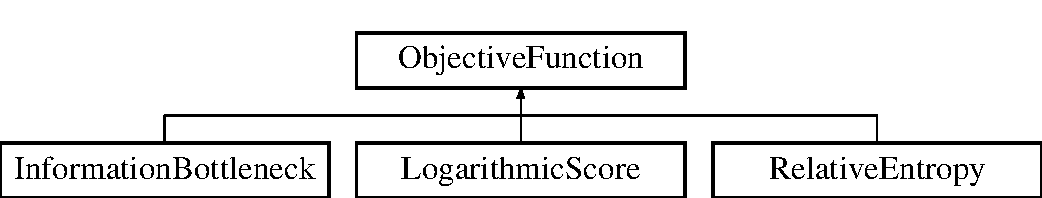
\includegraphics[height=2.000000cm]{classObjectiveFunction}
\end{center}
\end{figure}
\subsection*{Public Member Functions}
\begin{DoxyCompactItemize}
\item 
\hypertarget{classObjectiveFunction_a897009c58cc55bc84c29e5e3a2bfcb61}{virtual void {\bfseries set\-Random} ()=0}\label{classObjectiveFunction_a897009c58cc55bc84c29e5e3a2bfcb61}

\item 
\hypertarget{classObjectiveFunction_a4d302f7cdf40ca80d6d186cbf8851b8f}{virtual \hyperlink{classObjectiveValue}{Objective\-Value} $\ast$ {\bfseries new\-Objective\-Value} (int index=-\/1)=0}\label{classObjectiveFunction_a4d302f7cdf40ca80d6d186cbf8851b8f}

\item 
\hypertarget{classObjectiveFunction_a517095eb98863d0727a768d92fe2da0f}{virtual void {\bfseries compute\-Objective\-Values} ()=0}\label{classObjectiveFunction_a517095eb98863d0727a768d92fe2da0f}

\item 
\hypertarget{classObjectiveFunction_a7c59c162ea11841ade84d62fd29f0694}{virtual void {\bfseries print\-Objective\-Values} (bool verbose=true)=0}\label{classObjectiveFunction_a7c59c162ea11841ade84d62fd29f0694}

\item 
\hypertarget{classObjectiveFunction_a33d5014b560a6bb540558d25595b7c35}{virtual double {\bfseries get\-Parameter} (double unit)=0}\label{classObjectiveFunction_a33d5014b560a6bb540558d25595b7c35}

\item 
\hypertarget{classObjectiveFunction_abf21d384a51182fd183a580c1a4a5962}{virtual double {\bfseries get\-Unit\-Distance} (double u\-Min, double u\-Max)=0}\label{classObjectiveFunction_abf21d384a51182fd183a580c1a4a5962}

\item 
\hypertarget{classObjectiveFunction_ac554fa0076afa2d68a544e626e2e28a2}{virtual double {\bfseries get\-Intermediary\-Unit} (double u\-Min, double u\-Max)=0}\label{classObjectiveFunction_ac554fa0076afa2d68a544e626e2e28a2}

\end{DoxyCompactItemize}
\subsection*{Public Attributes}
\begin{DoxyCompactItemize}
\item 
\hypertarget{classObjectiveFunction_a325f3c8284ebfac0a170e0b8143dd7b5}{bool {\bfseries maximize}}\label{classObjectiveFunction_a325f3c8284ebfac0a170e0b8143dd7b5}

\end{DoxyCompactItemize}


The documentation for this class was generated from the following files\-:\begin{DoxyCompactItemize}
\item 
/home/lamarche/programming/optimal\-\_\-partition/src/objective\-\_\-function.\-hpp\item 
/home/lamarche/programming/optimal\-\_\-partition/src/objective\-\_\-function.\-cpp\end{DoxyCompactItemize}

\hypertarget{classObjectiveValue}{\section{Objective\-Value Class Reference}
\label{classObjectiveValue}\index{Objective\-Value@{Objective\-Value}}
}
Inheritance diagram for Objective\-Value\-:\begin{figure}[H]
\begin{center}
\leavevmode
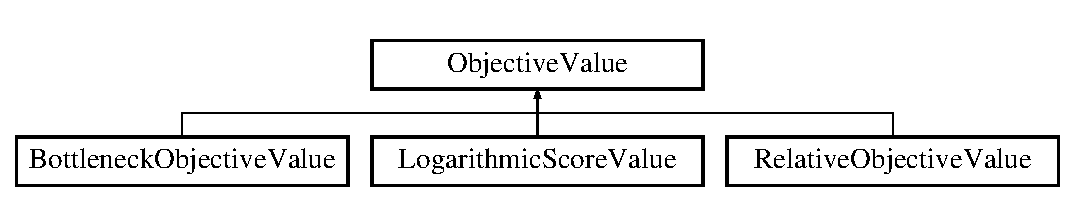
\includegraphics[height=2.000000cm]{classObjectiveValue}
\end{center}
\end{figure}
\subsection*{Public Member Functions}
\begin{DoxyCompactItemize}
\item 
\hypertarget{classObjectiveValue_a7934b001389d8b3a878958185b3e90d2}{virtual void {\bfseries add} (\hyperlink{classObjectiveValue}{Objective\-Value} $\ast$value)=0}\label{classObjectiveValue_a7934b001389d8b3a878958185b3e90d2}

\item 
\hypertarget{classObjectiveValue_ace4d2a545a72d9aa0572b56399785fb1}{virtual void {\bfseries compute} ()=0}\label{classObjectiveValue_ace4d2a545a72d9aa0572b56399785fb1}

\item 
\hypertarget{classObjectiveValue_aae11a5498d540f284ebed40584f09bd8}{virtual void {\bfseries compute} (\hyperlink{classObjectiveValue}{Objective\-Value} $\ast$value1, \hyperlink{classObjectiveValue}{Objective\-Value} $\ast$value2)=0}\label{classObjectiveValue_aae11a5498d540f284ebed40584f09bd8}

\item 
\hypertarget{classObjectiveValue_ab233604d149e5f4b8aa51ee34cba3292}{virtual void {\bfseries compute} (Objective\-Value\-Set $\ast$value\-Set)=0}\label{classObjectiveValue_ab233604d149e5f4b8aa51ee34cba3292}

\item 
\hypertarget{classObjectiveValue_afc703a4fb0d79ddd7904b339bd5e4934}{virtual void {\bfseries normalize} (\hyperlink{classObjectiveValue}{Objective\-Value} $\ast$normalizing\-Value)=0}\label{classObjectiveValue_afc703a4fb0d79ddd7904b339bd5e4934}

\item 
\hypertarget{classObjectiveValue_a66e0b4fdf1fc3bbab51ea9877aa1f7be}{virtual double {\bfseries get\-Value} (double param)=0}\label{classObjectiveValue_a66e0b4fdf1fc3bbab51ea9877aa1f7be}

\item 
\hypertarget{classObjectiveValue_a28afe825b3e9367fac69b3344bacb6a9}{virtual void {\bfseries print} (bool verbose=true)=0}\label{classObjectiveValue_a28afe825b3e9367fac69b3344bacb6a9}

\end{DoxyCompactItemize}
\subsection*{Public Attributes}
\begin{DoxyCompactItemize}
\item 
\hypertarget{classObjectiveValue_a12509b8168294b3b1a76ec092dd48a3a}{\hyperlink{classObjectiveFunction}{Objective\-Function} $\ast$ {\bfseries objective}}\label{classObjectiveValue_a12509b8168294b3b1a76ec092dd48a3a}

\end{DoxyCompactItemize}


The documentation for this class was generated from the following files\-:\begin{DoxyCompactItemize}
\item 
src/\hyperlink{objective__function_8hpp}{objective\-\_\-function.\-hpp}\item 
src/objective\-\_\-function.\-cpp\end{DoxyCompactItemize}

\hypertarget{classOrderedDatatree}{\section{Ordered\-Datatree Class Reference}
\label{classOrderedDatatree}\index{Ordered\-Datatree@{Ordered\-Datatree}}
}
\subsection*{Public Member Functions}
\begin{DoxyCompactItemize}
\item 
\hypertarget{classOrderedDatatree_a4f5024cc174646dc6483837c8c68d4d2}{{\bfseries Ordered\-Datatree} (\hyperlink{classOrderedDatatree}{Ordered\-Datatree} \&tree)}\label{classOrderedDatatree_a4f5024cc174646dc6483837c8c68d4d2}

\item 
\hypertarget{classOrderedDatatree_a7bb3bcab1152a0c854732730b3dd49a6}{{\bfseries Ordered\-Datatree} (int size2, int vertex=-\/1)}\label{classOrderedDatatree_a7bb3bcab1152a0c854732730b3dd49a6}

\item 
\hypertarget{classOrderedDatatree_a1a7cb343fd2dcab52df688dc1bbeea1f}{void {\bfseries set\-Objective\-Function} (\hyperlink{classObjectiveFunction}{Objective\-Function} $\ast$objective)}\label{classOrderedDatatree_a1a7cb343fd2dcab52df688dc1bbeea1f}

\item 
\hypertarget{classOrderedDatatree_acf3338e3b1201255fa2e3192843fc2ae}{Vertices $\ast$ {\bfseries get\-All\-Vertices} ()}\label{classOrderedDatatree_acf3338e3b1201255fa2e3192843fc2ae}

\item 
\hypertarget{classOrderedDatatree_a9bdc569ae3ede6fa3e027e3b37a8ff67}{int {\bfseries get\-Index} (int i, int j)}\label{classOrderedDatatree_a9bdc569ae3ede6fa3e027e3b37a8ff67}

\item 
\hypertarget{classOrderedDatatree_a503694e44cb7db99f290df984fb634a0}{\hyperlink{classOrderedDatatree}{Ordered\-Datatree} $\ast$ {\bfseries add\-Child} (int v, bool print=true)}\label{classOrderedDatatree_a503694e44cb7db99f290df984fb634a0}

\item 
\hypertarget{classOrderedDatatree_a4a88ab578cc74fb596b12a07adf39b46}{\hyperlink{classOrderedDatatree}{Ordered\-Datatree} $\ast$ {\bfseries find\-Child} (int v)}\label{classOrderedDatatree_a4a88ab578cc74fb596b12a07adf39b46}

\item 
\hypertarget{classOrderedDatatree_a68c7b2e4c94bf5582af68a2ff1071fc3}{\hyperlink{classOrderedDatatree}{Ordered\-Datatree} $\ast$ {\bfseries find\-Or\-Add\-Child} (int v, bool print=true)}\label{classOrderedDatatree_a68c7b2e4c94bf5582af68a2ff1071fc3}

\item 
\hypertarget{classOrderedDatatree_a83c551cab2adf911b1f6157b156c5c0c}{void {\bfseries add\-Bipartition} (\hyperlink{classOrderedDatatree}{Ordered\-Datatree} $\ast$n1, \hyperlink{classOrderedDatatree}{Ordered\-Datatree} $\ast$n2)}\label{classOrderedDatatree_a83c551cab2adf911b1f6157b156c5c0c}

\item 
\hypertarget{classOrderedDatatree_ab70217712cdcda97073d43e00f256515}{void {\bfseries compute\-Objective\-Values} ()}\label{classOrderedDatatree_ab70217712cdcda97073d43e00f256515}

\item 
\hypertarget{classOrderedDatatree_a46a9b17a536cae078a011033ce3e0b80}{void {\bfseries normalize\-Objective\-Values} (\hyperlink{classObjectiveValue}{Objective\-Value} $\ast$max\-Objective\-Value=0)}\label{classOrderedDatatree_a46a9b17a536cae078a011033ce3e0b80}

\item 
\hypertarget{classOrderedDatatree_a9426c2ed6c867e7d1ce983cd4a3667c3}{void {\bfseries print\-Objective\-Values} ()}\label{classOrderedDatatree_a9426c2ed6c867e7d1ce983cd4a3667c3}

\item 
\hypertarget{classOrderedDatatree_aa977ce66823f7939e55d8c4243eb018f}{void {\bfseries build\-Optimal\-Partition} (\hyperlink{classPartition}{Partition} $\ast$partition, int pi=0, int pj=-\/1)}\label{classOrderedDatatree_aa977ce66823f7939e55d8c4243eb018f}

\item 
\hypertarget{classOrderedDatatree_a89d065a30305bbd2dbb3dd20ccae2466}{void {\bfseries compute\-Optimal\-Partition} (double parameter)}\label{classOrderedDatatree_a89d065a30305bbd2dbb3dd20ccae2466}

\item 
\hypertarget{classOrderedDatatree_a7fc372dc95a5002a26cc706ff7c324ba}{void {\bfseries print\-Optimal\-Partition} (double parameter)}\label{classOrderedDatatree_a7fc372dc95a5002a26cc706ff7c324ba}

\item 
\hypertarget{classOrderedDatatree_a58e7431601539e62f1e07c5a07cb221f}{\hyperlink{classPartition}{Partition} $\ast$ {\bfseries get\-Optimal\-Partition} (double parameter)}\label{classOrderedDatatree_a58e7431601539e62f1e07c5a07cb221f}

\item 
\hypertarget{classOrderedDatatree_a208c2e706add4d03d1767e2c51806742}{void {\bfseries print} (bool verbose=false)}\label{classOrderedDatatree_a208c2e706add4d03d1767e2c51806742}

\item 
\hypertarget{classOrderedDatatree_a06c9691fea194ae11f8248118074097b}{void {\bfseries print\-Vertices} (bool endl=true)}\label{classOrderedDatatree_a06c9691fea194ae11f8248118074097b}

\end{DoxyCompactItemize}
\subsection*{Public Attributes}
\begin{DoxyCompactItemize}
\item 
\hypertarget{classOrderedDatatree_ae43ff7e5e18dc71c7a55a298d97c3c9e}{int {\bfseries size1}}\label{classOrderedDatatree_ae43ff7e5e18dc71c7a55a298d97c3c9e}

\item 
\hypertarget{classOrderedDatatree_ae36f7a02a46bd62d7e5611381a4ec02b}{int {\bfseries size2}}\label{classOrderedDatatree_ae36f7a02a46bd62d7e5611381a4ec02b}

\item 
\hypertarget{classOrderedDatatree_a69e8d93d69e9af770d6771201d53bcc4}{int {\bfseries vertex}}\label{classOrderedDatatree_a69e8d93d69e9af770d6771201d53bcc4}

\item 
\hypertarget{classOrderedDatatree_a95c150c56a737a4507b82125fb38183b}{bool {\bfseries whole\-Set}}\label{classOrderedDatatree_a95c150c56a737a4507b82125fb38183b}

\item 
\hypertarget{classOrderedDatatree_aa8ced7811f4c53bec40e4a1bda7073fa}{\hyperlink{classObjectiveFunction}{Objective\-Function} $\ast$ {\bfseries objective}}\label{classOrderedDatatree_aa8ced7811f4c53bec40e4a1bda7073fa}

\item 
\hypertarget{classOrderedDatatree_a79536afa768f9ce4b61d8baff254556f}{\hyperlink{classOrderedDatatree}{Ordered\-Datatree} $\ast$ {\bfseries parent}}\label{classOrderedDatatree_a79536afa768f9ce4b61d8baff254556f}

\item 
\hypertarget{classOrderedDatatree_a252db75f9a9aecbf0694eb331fe188b4}{\hyperlink{classOrderedDatatree}{Ordered\-Datatree} $\ast$ {\bfseries complement}}\label{classOrderedDatatree_a252db75f9a9aecbf0694eb331fe188b4}

\item 
\hypertarget{classOrderedDatatree_a63e87e1bdc0eaa3226eaad811a53bae6}{Ordered\-Trees\-List $\ast$ {\bfseries complement\-List}}\label{classOrderedDatatree_a63e87e1bdc0eaa3226eaad811a53bae6}

\item 
\hypertarget{classOrderedDatatree_ac13f35e59ddcf32a3b9ec11ec2a756d9}{Ordered\-Trees\-Set $\ast$ {\bfseries children}}\label{classOrderedDatatree_ac13f35e59ddcf32a3b9ec11ec2a756d9}

\item 
\hypertarget{classOrderedDatatree_a9bbd6bd520a9f0cf54da91c30b35c09e}{Ordered\-Bipartitions\-Set $\ast$ {\bfseries bipartitions}}\label{classOrderedDatatree_a9bbd6bd520a9f0cf54da91c30b35c09e}

\item 
\hypertarget{classOrderedDatatree_a3a1536573ceb5e61d8b271a1ebe9f44f}{\hyperlink{classObjectiveValue}{Objective\-Value} $\ast$$\ast$ {\bfseries qualities}}\label{classOrderedDatatree_a3a1536573ceb5e61d8b271a1ebe9f44f}

\item 
\hypertarget{classOrderedDatatree_a0bb2c4a9111b12dd2266ece96ffc836a}{double $\ast$ {\bfseries optimal\-Values}}\label{classOrderedDatatree_a0bb2c4a9111b12dd2266ece96ffc836a}

\item 
\hypertarget{classOrderedDatatree_a433aa570b06cb85e74b696b66a21c503}{int $\ast$ {\bfseries optimal\-Cuts}}\label{classOrderedDatatree_a433aa570b06cb85e74b696b66a21c503}

\item 
\hypertarget{classOrderedDatatree_a158f9eef6ebd0b9f66a15663f39439b5}{Ordered\-Bipartition $\ast$$\ast$ {\bfseries optimal\-Bipartitions}}\label{classOrderedDatatree_a158f9eef6ebd0b9f66a15663f39439b5}

\item 
\hypertarget{classOrderedDatatree_ac30581d76d9967d61ed9b5b66b1fb967}{bool {\bfseries optimized}}\label{classOrderedDatatree_ac30581d76d9967d61ed9b5b66b1fb967}

\end{DoxyCompactItemize}


The documentation for this class was generated from the following files\-:\begin{DoxyCompactItemize}
\item 
src/datatree.\-hpp\item 
src/datatree.\-cpp\end{DoxyCompactItemize}

\hypertarget{classOrderedSet}{\section{Ordered\-Set Class Reference}
\label{classOrderedSet}\index{Ordered\-Set@{Ordered\-Set}}
}
Inheritance diagram for Ordered\-Set\-:\begin{figure}[H]
\begin{center}
\leavevmode
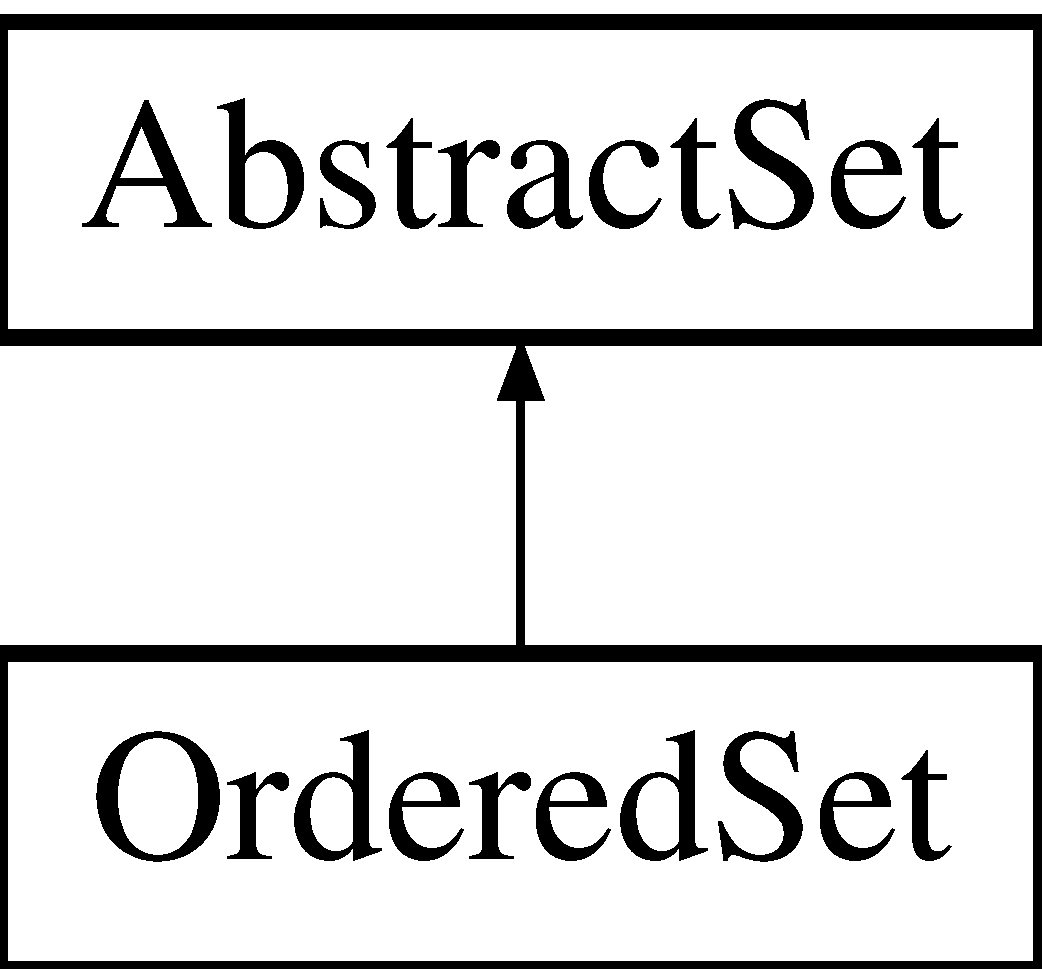
\includegraphics[height=2.000000cm]{classOrderedSet}
\end{center}
\end{figure}
\subsection*{Public Member Functions}
\begin{DoxyCompactItemize}
\item 
\hypertarget{classOrderedSet_a9cfaad9de53be413f85fadd9f25c8196}{{\bfseries Ordered\-Set} (int s)}\label{classOrderedSet_a9cfaad9de53be413f85fadd9f25c8196}

\item 
\hypertarget{classOrderedSet_a9b04f6f70c25ddfdb6539add1b806757}{int {\bfseries get\-Index} (int i, int j)}\label{classOrderedSet_a9b04f6f70c25ddfdb6539add1b806757}

\item 
\hypertarget{classOrderedSet_a907dcd3a18a9b363bf3150b4e28899bd}{void \hyperlink{classOrderedSet_a907dcd3a18a9b363bf3150b4e28899bd}{set\-Random} ()}\label{classOrderedSet_a907dcd3a18a9b363bf3150b4e28899bd}

\begin{DoxyCompactList}\small\item\em Randomly set the algebraic constraints for quick experiments (warning\-: this method is not always implemented) \end{DoxyCompactList}\item 
void \hyperlink{classOrderedSet_a6051e561b7b5fcd1dc5ee8f9f67353fe}{set\-Objective\-Function} (\hyperlink{classObjectiveFunction}{Objective\-Function} $\ast$m)
\begin{DoxyCompactList}\small\item\em Set the objective that one wants to optimise. \end{DoxyCompactList}\item 
\hypertarget{classOrderedSet_a3e1f7870eb9aeee5f6d74beab0786e37}{void \hyperlink{classOrderedSet_a3e1f7870eb9aeee5f6d74beab0786e37}{print} ()}\label{classOrderedSet_a3e1f7870eb9aeee5f6d74beab0786e37}

\begin{DoxyCompactList}\small\item\em Print the set and its algebraic constraints. \end{DoxyCompactList}\item 
\hypertarget{classOrderedSet_a6a9d6fdbf5ebcd43806a9f3e63126125}{void \hyperlink{classOrderedSet_a6a9d6fdbf5ebcd43806a9f3e63126125}{build\-Data\-Structure} ()}\label{classOrderedSet_a6a9d6fdbf5ebcd43806a9f3e63126125}

\begin{DoxyCompactList}\small\item\em Build a proper data structure to represent the set and its algebraic constraints (warning\-: this method should always be called after instantiating and parameterising a set, and before calling any other method, such as \hyperlink{classOrderedSet_a3e1f7870eb9aeee5f6d74beab0786e37}{print()}, \hyperlink{classOrderedSet_af3145e214c22b87a945988f5489d4aec}{compute\-Objective\-Values()}, compute\-Optimal\-Partition (double parameter), etc.) \end{DoxyCompactList}\item 
\hypertarget{classOrderedSet_af3145e214c22b87a945988f5489d4aec}{void \hyperlink{classOrderedSet_af3145e214c22b87a945988f5489d4aec}{compute\-Objective\-Values} ()}\label{classOrderedSet_af3145e214c22b87a945988f5489d4aec}

\begin{DoxyCompactList}\small\item\em Compute the value of the objective function for each feasible part (warning\-: set\-Objective\-Function (\hyperlink{classObjectiveFunction}{Objective\-Function} $\ast$objective) should have been called first) \end{DoxyCompactList}\item 
\hypertarget{classOrderedSet_afde0eaeefc1cda5945dd77112de30604}{void \hyperlink{classOrderedSet_afde0eaeefc1cda5945dd77112de30604}{normalize\-Objective\-Values} ()}\label{classOrderedSet_afde0eaeefc1cda5945dd77112de30604}

\begin{DoxyCompactList}\small\item\em Finish computing the value of the objective function for each feasible part when normalisation is required (warning\-: only after \hyperlink{classOrderedSet_af3145e214c22b87a945988f5489d4aec}{compute\-Objective\-Values()} has been called) \end{DoxyCompactList}\item 
\hypertarget{classOrderedSet_a79c1b186010d4e6c4b69167da0fbfaeb}{void \hyperlink{classOrderedSet_a79c1b186010d4e6c4b69167da0fbfaeb}{print\-Objective\-Values} ()}\label{classOrderedSet_a79c1b186010d4e6c4b69167da0fbfaeb}

\begin{DoxyCompactList}\small\item\em Print the value of the objective function for each feasible part. \end{DoxyCompactList}\item 
void \hyperlink{classOrderedSet_a2b17cd7170d713309d0ae39f0d18fd59}{compute\-Optimal\-Partition} (double parameter)
\begin{DoxyCompactList}\small\item\em Compute a partition that fits with the algebraic constraints and that optimises the objective function that has been specified. \end{DoxyCompactList}\item 
void \hyperlink{classOrderedSet_a14b48fdc9b30adb26a4c5d126160698e}{print\-Optimal\-Partition} (double parameter)
\begin{DoxyCompactList}\small\item\em Compute and print a partition that fits with the algebraic constraints and that optimises the objective function that has been specified (warning\-: this method is not always implemented, but one can obtain a similar result by using get\-Optimal\-Partition (double parameter) and by calling \hyperlink{classOrderedSet_a3e1f7870eb9aeee5f6d74beab0786e37}{print()} on the result) \end{DoxyCompactList}\item 
\hyperlink{classPartition}{Partition} $\ast$ \hyperlink{classOrderedSet_ac347be002f2b52ebc08ef6fdb6214f08}{get\-Optimal\-Partition} (double parameter)
\begin{DoxyCompactList}\small\item\em Compute and return a partition that fits with the algebraic constraints and that optimises the objective function that has been specified (warning\-: this method is not always implemented, but one can obtain a similar result by using get\-Optimal\-Partition (double parameter) and by calling \hyperlink{classOrderedSet_a3e1f7870eb9aeee5f6d74beab0786e37}{print()} on the result) \end{DoxyCompactList}\end{DoxyCompactItemize}
\subsection*{Public Attributes}
\begin{DoxyCompactItemize}
\item 
\hypertarget{classOrderedSet_a6a00f5e277235f5556a99c12a608691e}{int {\bfseries size}}\label{classOrderedSet_a6a00f5e277235f5556a99c12a608691e}

\item 
\hypertarget{classOrderedSet_a1379388c5b7f35edadf521ee96d08d1d}{\hyperlink{classObjectiveValue}{Objective\-Value} $\ast$$\ast$ {\bfseries qualities}}\label{classOrderedSet_a1379388c5b7f35edadf521ee96d08d1d}

\item 
\hypertarget{classOrderedSet_ab336fbe9cf14777f5f7bd77af65cab40}{double $\ast$ {\bfseries optimal\-Values}}\label{classOrderedSet_ab336fbe9cf14777f5f7bd77af65cab40}

\item 
\hypertarget{classOrderedSet_a3023782463777a76dfc0edfb632889f5}{int $\ast$ {\bfseries optimal\-Cuts}}\label{classOrderedSet_a3023782463777a76dfc0edfb632889f5}

\end{DoxyCompactItemize}


\subsection{Member Function Documentation}
\hypertarget{classOrderedSet_a2b17cd7170d713309d0ae39f0d18fd59}{\index{Ordered\-Set@{Ordered\-Set}!compute\-Optimal\-Partition@{compute\-Optimal\-Partition}}
\index{compute\-Optimal\-Partition@{compute\-Optimal\-Partition}!OrderedSet@{Ordered\-Set}}
\subsubsection[{compute\-Optimal\-Partition}]{\setlength{\rightskip}{0pt plus 5cm}void Ordered\-Set\-::compute\-Optimal\-Partition (
\begin{DoxyParamCaption}
\item[{double}]{parameter}
\end{DoxyParamCaption}
)\hspace{0.3cm}{\ttfamily [virtual]}}}\label{classOrderedSet_a2b17cd7170d713309d0ae39f0d18fd59}


Compute a partition that fits with the algebraic constraints and that optimises the objective function that has been specified. 


\begin{DoxyParams}{Parameters}
{\em parameter} & \-: The parameter of the objective function to be optimised (if the objective is parametrised) \\
\hline
\end{DoxyParams}


Implements \hyperlink{classAbstractSet_acfc3004f18192f38e32bb7a5a12ec8df}{Abstract\-Set}.

\hypertarget{classOrderedSet_ac347be002f2b52ebc08ef6fdb6214f08}{\index{Ordered\-Set@{Ordered\-Set}!get\-Optimal\-Partition@{get\-Optimal\-Partition}}
\index{get\-Optimal\-Partition@{get\-Optimal\-Partition}!OrderedSet@{Ordered\-Set}}
\subsubsection[{get\-Optimal\-Partition}]{\setlength{\rightskip}{0pt plus 5cm}{\bf Partition} $\ast$ Ordered\-Set\-::get\-Optimal\-Partition (
\begin{DoxyParamCaption}
\item[{double}]{parameter}
\end{DoxyParamCaption}
)\hspace{0.3cm}{\ttfamily [virtual]}}}\label{classOrderedSet_ac347be002f2b52ebc08ef6fdb6214f08}


Compute and return a partition that fits with the algebraic constraints and that optimises the objective function that has been specified (warning\-: this method is not always implemented, but one can obtain a similar result by using get\-Optimal\-Partition (double parameter) and by calling \hyperlink{classOrderedSet_a3e1f7870eb9aeee5f6d74beab0786e37}{print()} on the result) 


\begin{DoxyParams}{Parameters}
{\em parameter} & \-: The parameter of the objective function to be optimised (if the objective is parametrised) \\
\hline
\end{DoxyParams}
\begin{DoxyReturn}{Returns}
\-: The resulting optimal partition 
\end{DoxyReturn}


Implements \hyperlink{classAbstractSet_a48fd08c4b61ed46946bed6e19cd11194}{Abstract\-Set}.

\hypertarget{classOrderedSet_a14b48fdc9b30adb26a4c5d126160698e}{\index{Ordered\-Set@{Ordered\-Set}!print\-Optimal\-Partition@{print\-Optimal\-Partition}}
\index{print\-Optimal\-Partition@{print\-Optimal\-Partition}!OrderedSet@{Ordered\-Set}}
\subsubsection[{print\-Optimal\-Partition}]{\setlength{\rightskip}{0pt plus 5cm}void Ordered\-Set\-::print\-Optimal\-Partition (
\begin{DoxyParamCaption}
\item[{double}]{parameter}
\end{DoxyParamCaption}
)\hspace{0.3cm}{\ttfamily [virtual]}}}\label{classOrderedSet_a14b48fdc9b30adb26a4c5d126160698e}


Compute and print a partition that fits with the algebraic constraints and that optimises the objective function that has been specified (warning\-: this method is not always implemented, but one can obtain a similar result by using get\-Optimal\-Partition (double parameter) and by calling \hyperlink{classOrderedSet_a3e1f7870eb9aeee5f6d74beab0786e37}{print()} on the result) 


\begin{DoxyParams}{Parameters}
{\em parameter} & \-: The parameter of the objective function to be optimised (if the objective is parametrised) \\
\hline
\end{DoxyParams}


Implements \hyperlink{classAbstractSet_a82a9ce5c2d30690f0d1b83b034e92e1e}{Abstract\-Set}.

\hypertarget{classOrderedSet_a6051e561b7b5fcd1dc5ee8f9f67353fe}{\index{Ordered\-Set@{Ordered\-Set}!set\-Objective\-Function@{set\-Objective\-Function}}
\index{set\-Objective\-Function@{set\-Objective\-Function}!OrderedSet@{Ordered\-Set}}
\subsubsection[{set\-Objective\-Function}]{\setlength{\rightskip}{0pt plus 5cm}void Ordered\-Set\-::set\-Objective\-Function (
\begin{DoxyParamCaption}
\item[{{\bf Objective\-Function} $\ast$}]{objective}
\end{DoxyParamCaption}
)\hspace{0.3cm}{\ttfamily [virtual]}}}\label{classOrderedSet_a6051e561b7b5fcd1dc5ee8f9f67353fe}


Set the objective that one wants to optimise. 


\begin{DoxyParams}{Parameters}
{\em objective} & \-: The objective function itself \\
\hline
\end{DoxyParams}


Implements \hyperlink{classAbstractSet_a7aef71679a18ab7965d1098da15b26c2}{Abstract\-Set}.



The documentation for this class was generated from the following files\-:\begin{DoxyCompactItemize}
\item 
/home/lamarche/programming/optimal\-\_\-partition/src/orderedset.\-hpp\item 
/home/lamarche/programming/optimal\-\_\-partition/src/orderedset.\-cpp\end{DoxyCompactItemize}

\hypertarget{classOrderedStructure}{\section{Ordered\-Structure Class Reference}
\label{classOrderedStructure}\index{Ordered\-Structure@{Ordered\-Structure}}
}
Inheritance diagram for Ordered\-Structure\-:\begin{figure}[H]
\begin{center}
\leavevmode
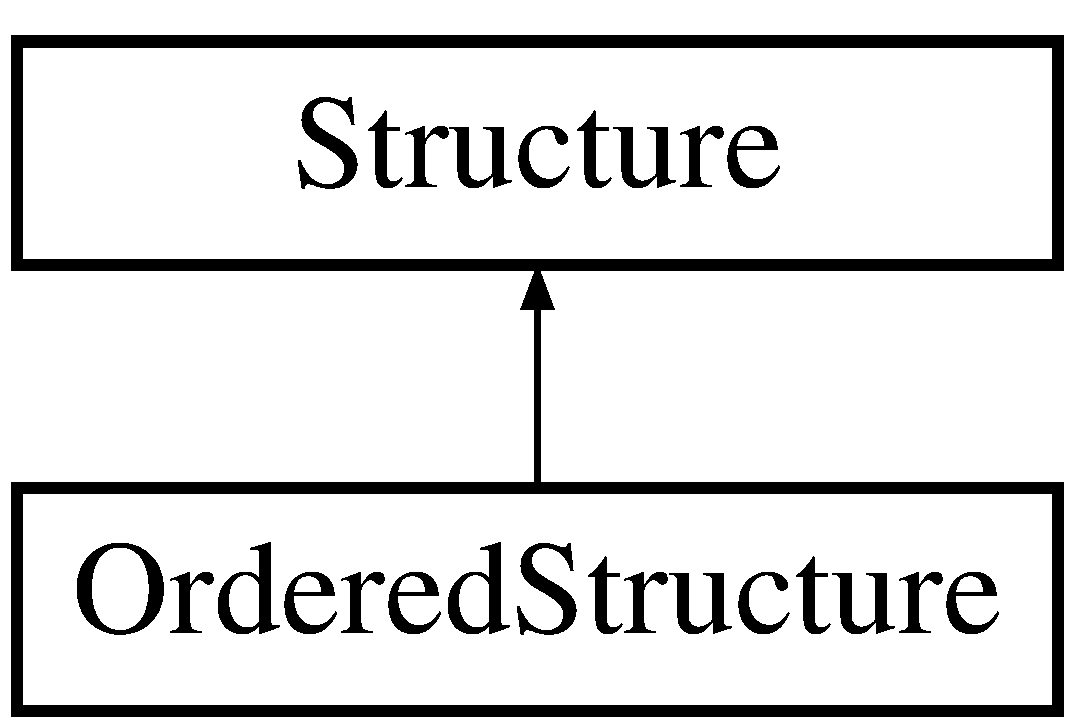
\includegraphics[height=2.000000cm]{classOrderedStructure}
\end{center}
\end{figure}
\subsection*{Public Member Functions}
\begin{DoxyCompactItemize}
\item 
\hypertarget{classOrderedStructure_a19e7ae039ef4d446da2bbdde91c21cfb}{{\bfseries Ordered\-Structure} (int size)}\label{classOrderedStructure_a19e7ae039ef4d446da2bbdde91c21cfb}

\item 
\hypertarget{classOrderedStructure_a1a07c725bb6bbea25dc4b529a68bfb5c}{int {\bfseries get\-Index} (int i, int j)}\label{classOrderedStructure_a1a07c725bb6bbea25dc4b529a68bfb5c}

\end{DoxyCompactItemize}
\subsection*{Public Attributes}
\begin{DoxyCompactItemize}
\item 
\hypertarget{classOrderedStructure_ab242085ce98312c82da735eabd9eaa22}{int {\bfseries size}}\label{classOrderedStructure_ab242085ce98312c82da735eabd9eaa22}

\end{DoxyCompactItemize}


The documentation for this class was generated from the following files\-:\begin{DoxyCompactItemize}
\item 
/home/lamarche/programming/optimal\-\_\-partition/src/structure.\-hpp\item 
/home/lamarche/programming/optimal\-\_\-partition/src/structure.\-cpp\end{DoxyCompactItemize}

\hypertarget{classPart}{\section{Part Class Reference}
\label{classPart}\index{Part@{Part}}
}


A part is a subset of a set of elements (individuals) represented by integers.  




{\ttfamily \#include $<$partition.\-hpp$>$}

Inheritance diagram for Part\-:\begin{figure}[H]
\begin{center}
\leavevmode
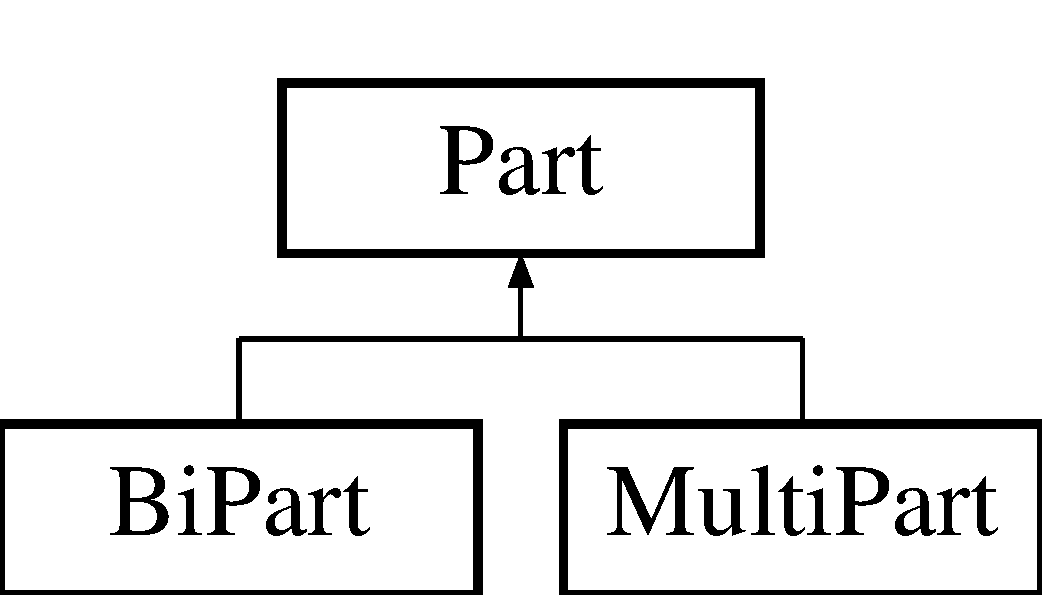
\includegraphics[height=2.000000cm]{classPart}
\end{center}
\end{figure}
\subsection*{Public Member Functions}
\begin{DoxyCompactItemize}
\item 
\hypertarget{classPart_a529e3046eef59e036be4a28293e1d696}{{\bfseries Part} (\hyperlink{classObjectiveValue}{Objective\-Value} $\ast$value=0)}\label{classPart_a529e3046eef59e036be4a28293e1d696}

\item 
\hypertarget{classPart_a4fc5eedff4d310041e3ebee54693f4ac}{{\bfseries Part} (\hyperlink{classPart}{Part} $\ast$part)}\label{classPart_a4fc5eedff4d310041e3ebee54693f4ac}

\item 
\hypertarget{classPart_abbe62c3accdcc1234035cd8149b540f0}{{\bfseries Part} (\hyperlink{classDatatree}{Datatree} $\ast$node, \hyperlink{classObjectiveValue}{Objective\-Value} $\ast$value=0)}\label{classPart_abbe62c3accdcc1234035cd8149b540f0}

\item 
\hypertarget{classPart_aa711a575b6b5bb0080b4e9fa7e20bbe1}{void {\bfseries add\-Individual} (int i, bool front=false)}\label{classPart_aa711a575b6b5bb0080b4e9fa7e20bbe1}

\item 
\hypertarget{classPart_aa5a500dd200b320ffd3a51868cc79fb0}{Vertices $\ast$ {\bfseries get\-Vertices} ()}\label{classPart_aa5a500dd200b320ffd3a51868cc79fb0}

\item 
\hypertarget{classPart_a8b37a2433f60fba0c5dcce393e4f5a86}{virtual bool {\bfseries equal} (\hyperlink{classPart}{Part} $\ast$p)}\label{classPart_a8b37a2433f60fba0c5dcce393e4f5a86}

\item 
\hypertarget{classPart_a2d3c13012c781d8651b820e60d57c724}{virtual void {\bfseries print} (bool endl=false)}\label{classPart_a2d3c13012c781d8651b820e60d57c724}

\item 
\hypertarget{classPart_a501f9fdbc4efd9ce00e1eef4a07f033e}{virtual int {\bfseries print\-Size} ()}\label{classPart_a501f9fdbc4efd9ce00e1eef4a07f033e}

\end{DoxyCompactItemize}
\subsection*{Public Attributes}
\begin{DoxyCompactItemize}
\item 
\hypertarget{classPart_a12f364b91efb5702af492cbdef1990fe}{std\-::list$<$ int $>$ $\ast$ {\bfseries individuals}}\label{classPart_a12f364b91efb5702af492cbdef1990fe}

\item 
\hypertarget{classPart_af9f5786f51cc11cffcf5c77ea656ae40}{\hyperlink{classObjectiveValue}{Objective\-Value} $\ast$ {\bfseries value}}\label{classPart_af9f5786f51cc11cffcf5c77ea656ae40}

\end{DoxyCompactItemize}


\subsection{Detailed Description}
A part is a subset of a set of elements (individuals) represented by integers. 

The documentation for this class was generated from the following files\-:\begin{DoxyCompactItemize}
\item 
/home/lamarche/programming/optimal\-\_\-partition/src/partition.\-hpp\item 
/home/lamarche/programming/optimal\-\_\-partition/src/partition.\-cpp\end{DoxyCompactItemize}

\hypertarget{classPartition}{\section{Partition Class Reference}
\label{classPartition}\index{Partition@{Partition}}
}


A partition is a collection of pairwise-\/disjoint and covering subsets (parts) of a set of elements.  




{\ttfamily \#include $<$partition.\-hpp$>$}

\subsection*{Public Member Functions}
\begin{DoxyCompactItemize}
\item 
\hypertarget{classPartition_ab2274b9cf773fea65da75facdf88ae98}{{\bfseries Partition} (\hyperlink{classObjectiveFunction}{Objective\-Function} $\ast$objective=0, double parameter=0)}\label{classPartition_ab2274b9cf773fea65da75facdf88ae98}

\item 
\hypertarget{classPartition_acb291b3b0ccf48005e141be32fdd7efd}{{\bfseries Partition} (\hyperlink{classPartition}{Partition} $\ast$partition)}\label{classPartition_acb291b3b0ccf48005e141be32fdd7efd}

\item 
\hypertarget{classPartition_a63f82a3a75dc0c3d0d27766b2459c9fe}{void {\bfseries add\-Part} (\hyperlink{classPart}{Part} $\ast$p, bool front=false)}\label{classPartition_a63f82a3a75dc0c3d0d27766b2459c9fe}

\item 
\hypertarget{classPartition_abced08b339e293866a614b2f21414375}{bool {\bfseries equal} (\hyperlink{classPartition}{Partition} $\ast$p)}\label{classPartition_abced08b339e293866a614b2f21414375}

\item 
\hypertarget{classPartition_a3463b34ab90d020ed40635c473301a64}{void {\bfseries print} (bool endl=false)}\label{classPartition_a3463b34ab90d020ed40635c473301a64}

\end{DoxyCompactItemize}
\subsection*{Public Attributes}
\begin{DoxyCompactItemize}
\item 
\hypertarget{classPartition_a1125b9b5548fa65e98a6dd94279c53bc}{double {\bfseries parameter}}\label{classPartition_a1125b9b5548fa65e98a6dd94279c53bc}

\item 
\hypertarget{classPartition_a887cae6498c54754779d7956b48e8d3e}{std\-::list$<$ \hyperlink{classPart}{Part} $\ast$ $>$ $\ast$ {\bfseries parts}}\label{classPartition_a887cae6498c54754779d7956b48e8d3e}

\item 
\hypertarget{classPartition_acb93c172b3e9a1bb4c6e0b1c5a50a13d}{\hyperlink{classObjectiveValue}{Objective\-Value} $\ast$ {\bfseries value}}\label{classPartition_acb93c172b3e9a1bb4c6e0b1c5a50a13d}

\end{DoxyCompactItemize}


\subsection{Detailed Description}
A partition is a collection of pairwise-\/disjoint and covering subsets (parts) of a set of elements. 

The documentation for this class was generated from the following files\-:\begin{DoxyCompactItemize}
\item 
/home/lamarche/programming/optimal\-\_\-partition/src/partition.\-hpp\item 
/home/lamarche/programming/optimal\-\_\-partition/src/partition.\-cpp\end{DoxyCompactItemize}

\hypertarget{classPredictionDataset}{\section{Prediction\-Dataset Class Reference}
\label{classPredictionDataset}\index{Prediction\-Dataset@{Prediction\-Dataset}}
}


Class to represent a data set for the prediction of a post-\/measurement from the knowledge of a pre-\/measurement (composed of a train set and a test set)  




{\ttfamily \#include $<$prediction\-\_\-dataset.\-hpp$>$}

\subsection*{Public Member Functions}
\begin{DoxyCompactItemize}
\item 
\hyperlink{classPredictionDataset_a5a2d75a4affa2b76dbb631f2f79c217e}{Prediction\-Dataset} (\hyperlink{classMultiSet}{Multi\-Set} $\ast$pre\-Measurement, \hyperlink{classMultiSet}{Multi\-Set} $\ast$post\-Measurement)
\begin{DoxyCompactList}\small\item\em The number of observations associated to a couple (pre-\/value, post-\/value) \end{DoxyCompactList}\item 
\hypertarget{classPredictionDataset_a9a30fa528fa4a2507a1a0a5fe8c74269}{\hyperlink{classPredictionDataset_a9a30fa528fa4a2507a1a0a5fe8c74269}{$\sim$\-Prediction\-Dataset} ()}\label{classPredictionDataset_a9a30fa528fa4a2507a1a0a5fe8c74269}

\begin{DoxyCompactList}\small\item\em Destructor. \end{DoxyCompactList}\item 
void \hyperlink{classPredictionDataset_adb6c93538580ea8ce7b482fc8bc6f6b7}{add\-Train\-Value} (double $\ast$pre\-Values, double $\ast$post\-Values, int count=1)
\begin{DoxyCompactList}\small\item\em Add a couple of (pre and post) observations to the train set {\bfseries in the case a range has been defined for all uni-\/dimensional sets} \end{DoxyCompactList}\item 
void \hyperlink{classPredictionDataset_ad9e633c08b0ab2af46248c6a66bf00ba}{add\-Test\-Value} (double $\ast$pre\-Values, double $\ast$post\-Values, int count=1)
\begin{DoxyCompactList}\small\item\em Add a couple of (pre and post) observations to the test set {\bfseries in the case a range has been defined for all uni-\/dimensional sets} \end{DoxyCompactList}\item 
void \hyperlink{classPredictionDataset_ae2d6c192122c2f9f7a1b3232b486d86c}{add\-Train\-Value} (\hyperlink{classMultiSubset}{Multi\-Subset} $\ast$pre\-Value, \hyperlink{classMultiSubset}{Multi\-Subset} $\ast$post\-Value, int count=1)
\begin{DoxyCompactList}\small\item\em Add a couple of (pre and post) observations to the train set. \end{DoxyCompactList}\item 
void \hyperlink{classPredictionDataset_a097fc45e897544af6b5215a26fa41527}{add\-Test\-Value} (\hyperlink{classMultiSubset}{Multi\-Subset} $\ast$pre\-Value, \hyperlink{classMultiSubset}{Multi\-Subset} $\ast$post\-Value, int count=1)
\begin{DoxyCompactList}\small\item\em Add a couple of (pre and post) observations to the test set. \end{DoxyCompactList}\item 
void \hyperlink{classPredictionDataset_a9615dd7ab9f8dd04fb2fb28d68bd96b1}{add\-Train\-Value} (int pre\-Index, int post\-Index, int count=1)
\begin{DoxyCompactList}\small\item\em Add a couple of (pre and post) observations to the train set {\bfseries in the case of one-\/dimensional measurements} \end{DoxyCompactList}\item 
void \hyperlink{classPredictionDataset_a8298f94fac0d5b3761effdb20405417a}{add\-Test\-Value} (int pre\-Index, int post\-Index, int count=1)
\begin{DoxyCompactList}\small\item\em Add a couple of (pre and post) observations to the test set {\bfseries in the case of one-\/dimensional measurements} \end{DoxyCompactList}\item 
void \hyperlink{classPredictionDataset_a2d4d421a0299c9f965965f1d3797316e}{print} ()
\end{DoxyCompactItemize}
\subsection*{Public Attributes}
\begin{DoxyCompactItemize}
\item 
\hypertarget{classPredictionDataset_a47b4d8ccf188271ce59ee481377a3c5f}{\hyperlink{classMultiSet}{Multi\-Set} $\ast$ {\bfseries pre\-Multi\-Set}}\label{classPredictionDataset_a47b4d8ccf188271ce59ee481377a3c5f}

\item 
\hypertarget{classPredictionDataset_a22343b4582412434376af66cb42d2d50}{\hyperlink{classMultiSet}{Multi\-Set} $\ast$ \hyperlink{classPredictionDataset_a22343b4582412434376af66cb42d2d50}{post\-Multi\-Set}}\label{classPredictionDataset_a22343b4582412434376af66cb42d2d50}

\begin{DoxyCompactList}\small\item\em The pre-\/measurement modelled as a structured multi-\/dimensional set of elements (the possible observation values) \end{DoxyCompactList}\item 
\hypertarget{classPredictionDataset_af09491db0c4267fa086bf640c4740483}{std\-::vector$<$ \hyperlink{classMultiSubset}{Multi\-Subset} $\ast$ $>$ $\ast$ \hyperlink{classPredictionDataset_af09491db0c4267fa086bf640c4740483}{train\-Pre\-Values}}\label{classPredictionDataset_af09491db0c4267fa086bf640c4740483}

\begin{DoxyCompactList}\small\item\em The post-\/measurement modelled as a structured multi-\/dimensional set of elements (the possible observation values) \end{DoxyCompactList}\item 
\hypertarget{classPredictionDataset_a30e9419638339a7497f3d234780b2c20}{std\-::vector$<$ \hyperlink{classMultiSubset}{Multi\-Subset} $\ast$ $>$ $\ast$ \hyperlink{classPredictionDataset_a30e9419638339a7497f3d234780b2c20}{train\-Post\-Values}}\label{classPredictionDataset_a30e9419638339a7497f3d234780b2c20}

\begin{DoxyCompactList}\small\item\em A vector of pre-\/observations that are used to train the predictor. \end{DoxyCompactList}\item 
\hypertarget{classPredictionDataset_af4fdcf7cfd236a99a73f18d630199291}{std\-::vector$<$ int $>$ $\ast$ \hyperlink{classPredictionDataset_af4fdcf7cfd236a99a73f18d630199291}{train\-Count\-Values}}\label{classPredictionDataset_af4fdcf7cfd236a99a73f18d630199291}

\begin{DoxyCompactList}\small\item\em A vector of post-\/observations that are used to train the predictor. \end{DoxyCompactList}\item 
\hypertarget{classPredictionDataset_a6ef1712f6f3e944cad7f966b123c44d4}{std\-::vector$<$ \hyperlink{classMultiSubset}{Multi\-Subset} $\ast$ $>$ $\ast$ \hyperlink{classPredictionDataset_a6ef1712f6f3e944cad7f966b123c44d4}{test\-Pre\-Values}}\label{classPredictionDataset_a6ef1712f6f3e944cad7f966b123c44d4}

\begin{DoxyCompactList}\small\item\em The number of observations associated to a couple (pre-\/value, post-\/value) \end{DoxyCompactList}\item 
\hypertarget{classPredictionDataset_ab6ed50cd17878109b9a41ebb6db172ea}{std\-::vector$<$ \hyperlink{classMultiSubset}{Multi\-Subset} $\ast$ $>$ $\ast$ \hyperlink{classPredictionDataset_ab6ed50cd17878109b9a41ebb6db172ea}{test\-Post\-Values}}\label{classPredictionDataset_ab6ed50cd17878109b9a41ebb6db172ea}

\begin{DoxyCompactList}\small\item\em A vector of pre-\/observations that are used to test the predictor. \end{DoxyCompactList}\item 
\hypertarget{classPredictionDataset_a7fe2eccbdae1cee136f5864b660c31ee}{std\-::vector$<$ int $>$ $\ast$ \hyperlink{classPredictionDataset_a7fe2eccbdae1cee136f5864b660c31ee}{test\-Count\-Values}}\label{classPredictionDataset_a7fe2eccbdae1cee136f5864b660c31ee}

\begin{DoxyCompactList}\small\item\em A vector of post-\/observations that are used to test the predictor. \end{DoxyCompactList}\end{DoxyCompactItemize}


\subsection{Detailed Description}
Class to represent a data set for the prediction of a post-\/measurement from the knowledge of a pre-\/measurement (composed of a train set and a test set) 

\subsection{Constructor \& Destructor Documentation}
\hypertarget{classPredictionDataset_a5a2d75a4affa2b76dbb631f2f79c217e}{\index{Prediction\-Dataset@{Prediction\-Dataset}!Prediction\-Dataset@{Prediction\-Dataset}}
\index{Prediction\-Dataset@{Prediction\-Dataset}!PredictionDataset@{Prediction\-Dataset}}
\subsubsection[{Prediction\-Dataset}]{\setlength{\rightskip}{0pt plus 5cm}Prediction\-Dataset\-::\-Prediction\-Dataset (
\begin{DoxyParamCaption}
\item[{{\bf Multi\-Set} $\ast$}]{pre\-Measurement, }
\item[{{\bf Multi\-Set} $\ast$}]{post\-Measurement}
\end{DoxyParamCaption}
)}}\label{classPredictionDataset_a5a2d75a4affa2b76dbb631f2f79c217e}


The number of observations associated to a couple (pre-\/value, post-\/value) 

Constructor 
\begin{DoxyParams}{Parameters}
{\em pre\-Measurement} & \-: The pre-\/measurement modelled as a structured multi-\/dimensional set of elements (the possible observation values) \\
\hline
{\em post\-Measurement} & \-: The post-\/measurement modelled as a structured multi-\/dimensional set of elements (the possible observation values) \\
\hline
\end{DoxyParams}


\subsection{Member Function Documentation}
\hypertarget{classPredictionDataset_ad9e633c08b0ab2af46248c6a66bf00ba}{\index{Prediction\-Dataset@{Prediction\-Dataset}!add\-Test\-Value@{add\-Test\-Value}}
\index{add\-Test\-Value@{add\-Test\-Value}!PredictionDataset@{Prediction\-Dataset}}
\subsubsection[{add\-Test\-Value}]{\setlength{\rightskip}{0pt plus 5cm}void Prediction\-Dataset\-::add\-Test\-Value (
\begin{DoxyParamCaption}
\item[{double $\ast$}]{pre\-Values, }
\item[{double $\ast$}]{post\-Values, }
\item[{int}]{count = {\ttfamily 1}}
\end{DoxyParamCaption}
)}}\label{classPredictionDataset_ad9e633c08b0ab2af46248c6a66bf00ba}


Add a couple of (pre and post) observations to the test set {\bfseries in the case a range has been defined for all uni-\/dimensional sets} 


\begin{DoxyParams}{Parameters}
{\em pre\-Values} & \-: An array of real values that have been pre-\/observed, thus referring to uni-\/dimensional elements in the pre-\/measurement \\
\hline
{\em post\-Values} & \-: An array of real values that have been post-\/observed, thus referring to uni-\/dimensional elements in the post-\/measurement \\
\hline
{\em count} & \-: The number of times the couple has been observed \\
\hline
\end{DoxyParams}
\hypertarget{classPredictionDataset_a097fc45e897544af6b5215a26fa41527}{\index{Prediction\-Dataset@{Prediction\-Dataset}!add\-Test\-Value@{add\-Test\-Value}}
\index{add\-Test\-Value@{add\-Test\-Value}!PredictionDataset@{Prediction\-Dataset}}
\subsubsection[{add\-Test\-Value}]{\setlength{\rightskip}{0pt plus 5cm}void Prediction\-Dataset\-::add\-Test\-Value (
\begin{DoxyParamCaption}
\item[{{\bf Multi\-Subset} $\ast$}]{pre\-Value, }
\item[{{\bf Multi\-Subset} $\ast$}]{post\-Value, }
\item[{int}]{count = {\ttfamily 1}}
\end{DoxyParamCaption}
)}}\label{classPredictionDataset_a097fc45e897544af6b5215a26fa41527}


Add a couple of (pre and post) observations to the test set. 


\begin{DoxyParams}{Parameters}
{\em pre\-Value} & \-: A pointer to the feasible subset that has been pre-\/observed in the multi-\/dimensional set representing the pre-\/measurement. It should always be an element of the set, that is an atomic feasible subset \\
\hline
{\em pre\-Value} & \-: A pointer to the feasible subset that has been post-\/observed in the multi-\/dimensional set representing the pre-\/measurement. It should always be an element of the set, that is an atomic feasible subset \\
\hline
{\em count} & \-: The number of times the couple has been observed \\
\hline
\end{DoxyParams}
\hypertarget{classPredictionDataset_a8298f94fac0d5b3761effdb20405417a}{\index{Prediction\-Dataset@{Prediction\-Dataset}!add\-Test\-Value@{add\-Test\-Value}}
\index{add\-Test\-Value@{add\-Test\-Value}!PredictionDataset@{Prediction\-Dataset}}
\subsubsection[{add\-Test\-Value}]{\setlength{\rightskip}{0pt plus 5cm}void Prediction\-Dataset\-::add\-Test\-Value (
\begin{DoxyParamCaption}
\item[{int}]{pre\-Index, }
\item[{int}]{post\-Index, }
\item[{int}]{count = {\ttfamily 1}}
\end{DoxyParamCaption}
)}}\label{classPredictionDataset_a8298f94fac0d5b3761effdb20405417a}


Add a couple of (pre and post) observations to the test set {\bfseries in the case of one-\/dimensional measurements} 


\begin{DoxyParams}{Parameters}
{\em pre\-Index} & \-: The index of the element that has been pre-\/observed in the one-\/dimensional set representing the pre-\/measurement \\
\hline
{\em post\-Index} & \-: The index of the element that has been post-\/observed in the one-\/dimensional set representing the pre-\/measurement \\
\hline
{\em count} & \-: The number of times the couple has been observed \\
\hline
\end{DoxyParams}
\hypertarget{classPredictionDataset_adb6c93538580ea8ce7b482fc8bc6f6b7}{\index{Prediction\-Dataset@{Prediction\-Dataset}!add\-Train\-Value@{add\-Train\-Value}}
\index{add\-Train\-Value@{add\-Train\-Value}!PredictionDataset@{Prediction\-Dataset}}
\subsubsection[{add\-Train\-Value}]{\setlength{\rightskip}{0pt plus 5cm}void Prediction\-Dataset\-::add\-Train\-Value (
\begin{DoxyParamCaption}
\item[{double $\ast$}]{pre\-Values, }
\item[{double $\ast$}]{post\-Values, }
\item[{int}]{count = {\ttfamily 1}}
\end{DoxyParamCaption}
)}}\label{classPredictionDataset_adb6c93538580ea8ce7b482fc8bc6f6b7}


Add a couple of (pre and post) observations to the train set {\bfseries in the case a range has been defined for all uni-\/dimensional sets} 


\begin{DoxyParams}{Parameters}
{\em pre\-Values} & \-: An array of real values that have been pre-\/observed, thus referring to uni-\/dimensional elements in the pre-\/measurement \\
\hline
{\em post\-Values} & \-: An array of real values that have been post-\/observed, thus referring to uni-\/dimensional elements in the post-\/measurement \\
\hline
{\em count} & \-: The number of times the couple has been observed \\
\hline
\end{DoxyParams}
\hypertarget{classPredictionDataset_ae2d6c192122c2f9f7a1b3232b486d86c}{\index{Prediction\-Dataset@{Prediction\-Dataset}!add\-Train\-Value@{add\-Train\-Value}}
\index{add\-Train\-Value@{add\-Train\-Value}!PredictionDataset@{Prediction\-Dataset}}
\subsubsection[{add\-Train\-Value}]{\setlength{\rightskip}{0pt plus 5cm}void Prediction\-Dataset\-::add\-Train\-Value (
\begin{DoxyParamCaption}
\item[{{\bf Multi\-Subset} $\ast$}]{pre\-Value, }
\item[{{\bf Multi\-Subset} $\ast$}]{post\-Value, }
\item[{int}]{count = {\ttfamily 1}}
\end{DoxyParamCaption}
)}}\label{classPredictionDataset_ae2d6c192122c2f9f7a1b3232b486d86c}


Add a couple of (pre and post) observations to the train set. 


\begin{DoxyParams}{Parameters}
{\em pre\-Value} & \-: A pointer to the feasible subset that have been pre-\/observed in the multi-\/dimensional set representing the pre-\/measurement. It should always be an element of the set, that is an atomic feasible subset \\
\hline
{\em pre\-Value} & \-: A pointer to the feasible subset that have been post-\/observed in the multi-\/dimensional set representing the pre-\/measurement. It should always be an element of the set, that is an atomic feasible subset \\
\hline
{\em count} & \-: The number of times the couple has been observed \\
\hline
\end{DoxyParams}
\hypertarget{classPredictionDataset_a9615dd7ab9f8dd04fb2fb28d68bd96b1}{\index{Prediction\-Dataset@{Prediction\-Dataset}!add\-Train\-Value@{add\-Train\-Value}}
\index{add\-Train\-Value@{add\-Train\-Value}!PredictionDataset@{Prediction\-Dataset}}
\subsubsection[{add\-Train\-Value}]{\setlength{\rightskip}{0pt plus 5cm}void Prediction\-Dataset\-::add\-Train\-Value (
\begin{DoxyParamCaption}
\item[{int}]{pre\-Index, }
\item[{int}]{post\-Index, }
\item[{int}]{count = {\ttfamily 1}}
\end{DoxyParamCaption}
)}}\label{classPredictionDataset_a9615dd7ab9f8dd04fb2fb28d68bd96b1}


Add a couple of (pre and post) observations to the train set {\bfseries in the case of one-\/dimensional measurements} 


\begin{DoxyParams}{Parameters}
{\em pre\-Index} & \-: The index of the element that has been pre-\/observed in the one-\/dimensional set representing the pre-\/measurement \\
\hline
{\em post\-Index} & \-: The index of the element that has been post-\/observed in the one-\/dimensional set representing the pre-\/measurement \\
\hline
{\em count} & \-: The number of times the couple has been observed \\
\hline
\end{DoxyParams}
\hypertarget{classPredictionDataset_a2d4d421a0299c9f965965f1d3797316e}{\index{Prediction\-Dataset@{Prediction\-Dataset}!print@{print}}
\index{print@{print}!PredictionDataset@{Prediction\-Dataset}}
\subsubsection[{print}]{\setlength{\rightskip}{0pt plus 5cm}void Prediction\-Dataset\-::print (
\begin{DoxyParamCaption}
{}
\end{DoxyParamCaption}
)}}\label{classPredictionDataset_a2d4d421a0299c9f965965f1d3797316e}
/brief Print the data set. 

The documentation for this class was generated from the following files\-:\begin{DoxyCompactItemize}
\item 
src/\hyperlink{prediction__dataset_8hpp}{prediction\-\_\-dataset.\-hpp}\item 
src/prediction\-\_\-dataset.\-cpp\end{DoxyCompactItemize}

\hypertarget{classRandomGraph}{\section{Random\-Graph Class Reference}
\label{classRandomGraph}\index{Random\-Graph@{Random\-Graph}}
}
Inheritance diagram for Random\-Graph\-:\begin{figure}[H]
\begin{center}
\leavevmode
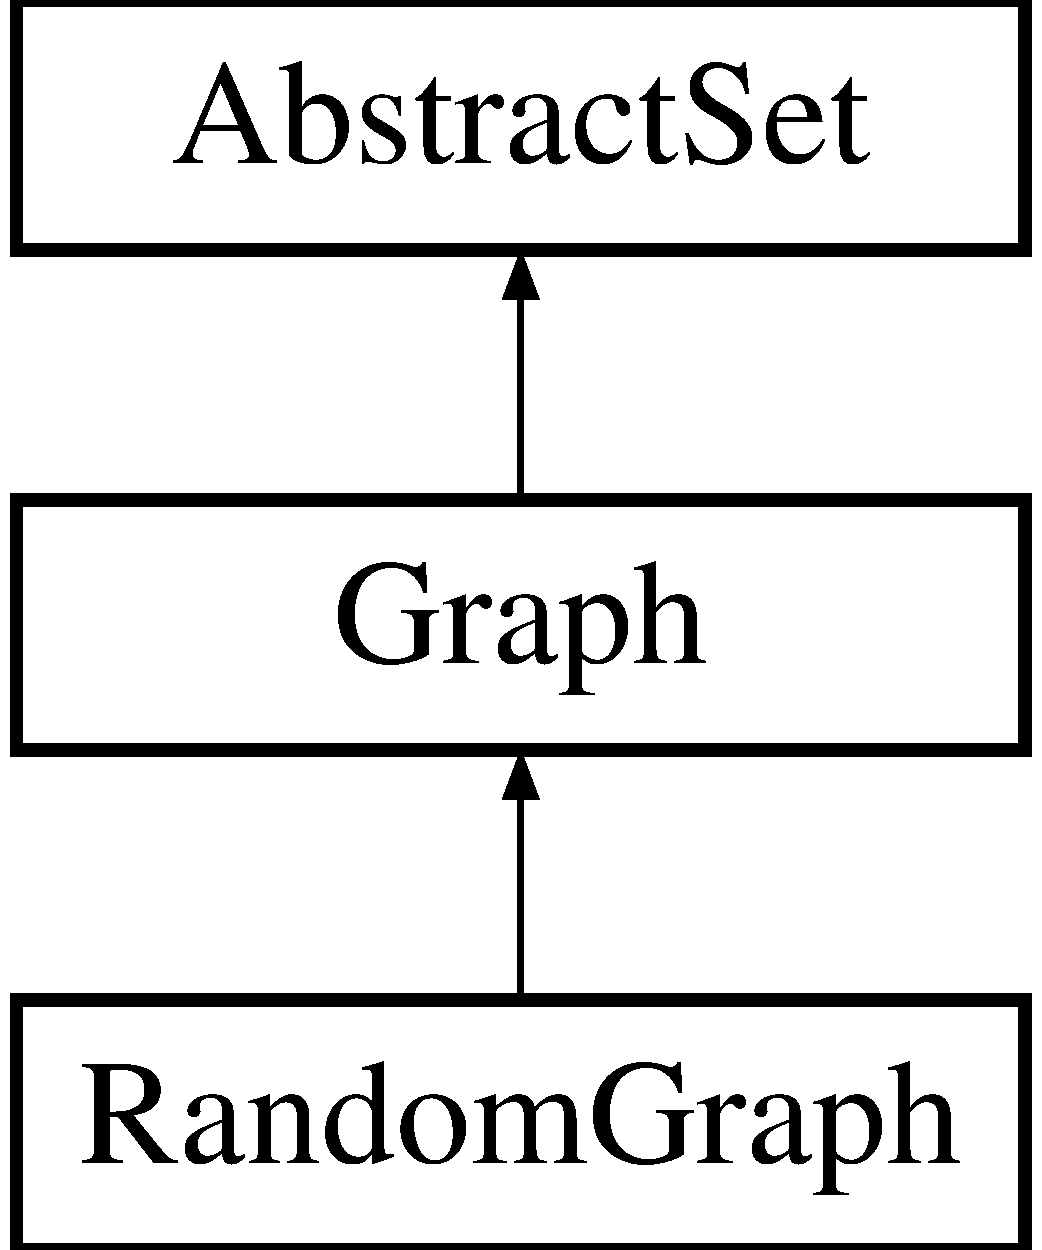
\includegraphics[height=3.000000cm]{classRandomGraph}
\end{center}
\end{figure}
\subsection*{Public Member Functions}
\begin{DoxyCompactItemize}
\item 
\hypertarget{classRandomGraph_aff05f804f75600257bf90455729b330f}{{\bfseries Random\-Graph} (int v\-Num, int e\-Num)}\label{classRandomGraph_aff05f804f75600257bf90455729b330f}

\end{DoxyCompactItemize}
\subsection*{Additional Inherited Members}


The documentation for this class was generated from the following files\-:\begin{DoxyCompactItemize}
\item 
src/graph.\-hpp\item 
src/graph.\-cpp\end{DoxyCompactItemize}

\hypertarget{classRelativeEntropy}{\section{Relative\-Entropy Class Reference}
\label{classRelativeEntropy}\index{Relative\-Entropy@{Relative\-Entropy}}
}
Inheritance diagram for Relative\-Entropy\-:\begin{figure}[H]
\begin{center}
\leavevmode
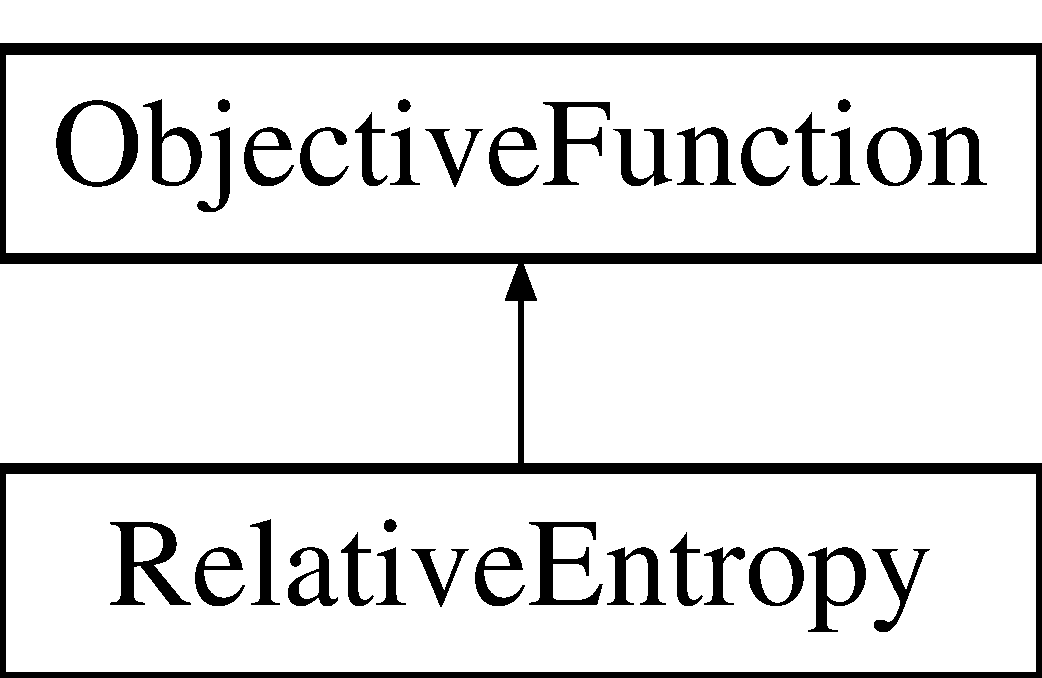
\includegraphics[height=2.000000cm]{classRelativeEntropy}
\end{center}
\end{figure}
\subsection*{Public Member Functions}
\begin{DoxyCompactItemize}
\item 
\hypertarget{classRelativeEntropy_a3681c506bf2071f11af6373ed2d2c570}{{\bfseries Relative\-Entropy} (int size, double $\ast$values=0, double $\ast$ref\-Values=0)}\label{classRelativeEntropy_a3681c506bf2071f11af6373ed2d2c570}

\item 
\hypertarget{classRelativeEntropy_aa34a724f03a10c7aa273cc6aa1444881}{void {\bfseries set\-Random} ()}\label{classRelativeEntropy_aa34a724f03a10c7aa273cc6aa1444881}

\item 
\hypertarget{classRelativeEntropy_a88c993870571948119498a5004879730}{\hyperlink{classObjectiveValue}{Objective\-Value} $\ast$ {\bfseries new\-Objective\-Value} (int index=-\/1)}\label{classRelativeEntropy_a88c993870571948119498a5004879730}

\item 
\hypertarget{classRelativeEntropy_ad2b1237540c333fc7bb7289579935598}{void {\bfseries compute\-Objective\-Values} ()}\label{classRelativeEntropy_ad2b1237540c333fc7bb7289579935598}

\item 
\hypertarget{classRelativeEntropy_affe7e822cc677fedfbc3ee259331763c}{void {\bfseries print\-Objective\-Values} (bool verbose=true)}\label{classRelativeEntropy_affe7e822cc677fedfbc3ee259331763c}

\item 
\hypertarget{classRelativeEntropy_ac021b7887e7ccb9d23a865ab3cdb0704}{double {\bfseries get\-Parameter} (double unit)}\label{classRelativeEntropy_ac021b7887e7ccb9d23a865ab3cdb0704}

\item 
\hypertarget{classRelativeEntropy_ab2173fffca585fc30bfe66ae2b3fd06a}{double {\bfseries get\-Unit\-Distance} (double u\-Min, double u\-Max)}\label{classRelativeEntropy_ab2173fffca585fc30bfe66ae2b3fd06a}

\item 
\hypertarget{classRelativeEntropy_a92c8e2ced62582fcd1dec801cedee04f}{double {\bfseries get\-Intermediary\-Unit} (double u\-Min, double u\-Max)}\label{classRelativeEntropy_a92c8e2ced62582fcd1dec801cedee04f}

\end{DoxyCompactItemize}
\subsection*{Public Attributes}
\begin{DoxyCompactItemize}
\item 
\hypertarget{classRelativeEntropy_a684e97eedbf983c173161693dbf89836}{int {\bfseries size}}\label{classRelativeEntropy_a684e97eedbf983c173161693dbf89836}

\item 
\hypertarget{classRelativeEntropy_abf8732d75d92b5e43deafba0b7a4d262}{double $\ast$ {\bfseries values}}\label{classRelativeEntropy_abf8732d75d92b5e43deafba0b7a4d262}

\item 
\hypertarget{classRelativeEntropy_a31d0f68b5478c06f9935e523c34e0df1}{double $\ast$ {\bfseries ref\-Values}}\label{classRelativeEntropy_a31d0f68b5478c06f9935e523c34e0df1}

\end{DoxyCompactItemize}


The documentation for this class was generated from the following files\-:\begin{DoxyCompactItemize}
\item 
/home/lamarche/programming/optimal\-\_\-partition/src/relative\-\_\-entropy.\-hpp\item 
/home/lamarche/programming/optimal\-\_\-partition/src/relative\-\_\-entropy.\-cpp\end{DoxyCompactItemize}

\hypertarget{classRelativeObjectiveValue}{\section{Relative\-Objective\-Value Class Reference}
\label{classRelativeObjectiveValue}\index{Relative\-Objective\-Value@{Relative\-Objective\-Value}}
}
Inheritance diagram for Relative\-Objective\-Value\-:\begin{figure}[H]
\begin{center}
\leavevmode
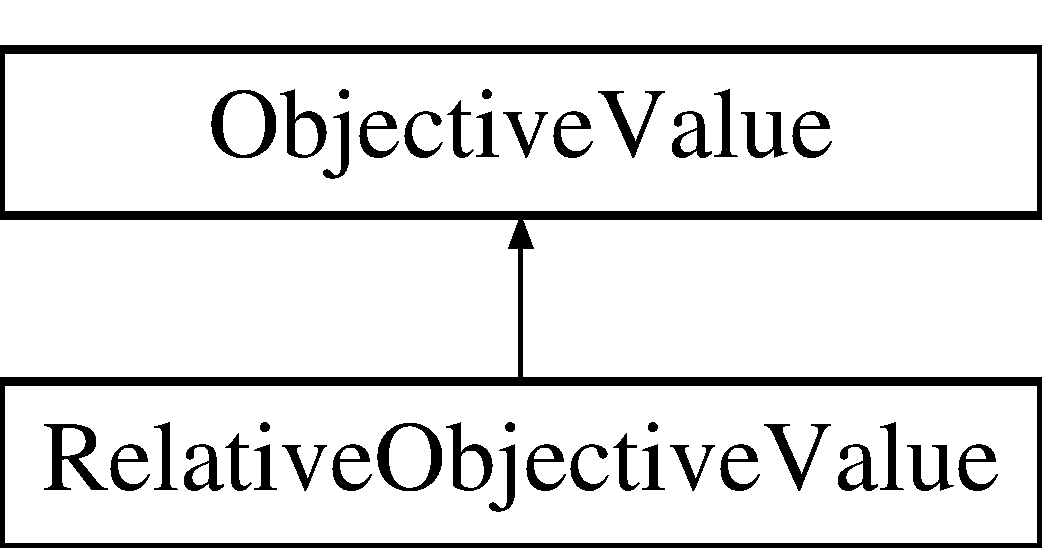
\includegraphics[height=2.000000cm]{classRelativeObjectiveValue}
\end{center}
\end{figure}
\subsection*{Public Member Functions}
\begin{DoxyCompactItemize}
\item 
\hypertarget{classRelativeObjectiveValue_a0cfe8e9aa6d2b5cbeca876cf16d5dd68}{{\bfseries Relative\-Objective\-Value} (\hyperlink{classRelativeEntropy}{Relative\-Entropy} $\ast$objective, int index=-\/1)}\label{classRelativeObjectiveValue_a0cfe8e9aa6d2b5cbeca876cf16d5dd68}

\item 
\hypertarget{classRelativeObjectiveValue_a7587c68ff0d7cba1d403824190493ab3}{void {\bfseries add} (\hyperlink{classObjectiveValue}{Objective\-Value} $\ast$value)}\label{classRelativeObjectiveValue_a7587c68ff0d7cba1d403824190493ab3}

\item 
\hypertarget{classRelativeObjectiveValue_af843a108184fffc1dbf42da6e4f68797}{void {\bfseries compute} ()}\label{classRelativeObjectiveValue_af843a108184fffc1dbf42da6e4f68797}

\item 
\hypertarget{classRelativeObjectiveValue_a9bbf0956cb2162f392487617563e40a0}{void {\bfseries compute} (\hyperlink{classObjectiveValue}{Objective\-Value} $\ast$value1, \hyperlink{classObjectiveValue}{Objective\-Value} $\ast$value2)}\label{classRelativeObjectiveValue_a9bbf0956cb2162f392487617563e40a0}

\item 
\hypertarget{classRelativeObjectiveValue_a25bca07f2785b8d2f925ca684566a66e}{void {\bfseries compute} (Objective\-Value\-Set $\ast$valueset)}\label{classRelativeObjectiveValue_a25bca07f2785b8d2f925ca684566a66e}

\item 
\hypertarget{classRelativeObjectiveValue_ac89fde7d4f6c8d63fb11f3fe48291f4a}{void {\bfseries normalize} (\hyperlink{classObjectiveValue}{Objective\-Value} $\ast$q)}\label{classRelativeObjectiveValue_ac89fde7d4f6c8d63fb11f3fe48291f4a}

\item 
\hypertarget{classRelativeObjectiveValue_ab8bb9d1464729e1b56a3d25a332e67b0}{void {\bfseries print} (bool verbose=true)}\label{classRelativeObjectiveValue_ab8bb9d1464729e1b56a3d25a332e67b0}

\item 
\hypertarget{classRelativeObjectiveValue_a85d36e917e1fef32dd11a657cb210d94}{double {\bfseries get\-Value} (double param)}\label{classRelativeObjectiveValue_a85d36e917e1fef32dd11a657cb210d94}

\end{DoxyCompactItemize}
\subsection*{Public Attributes}
\begin{DoxyCompactItemize}
\item 
\hypertarget{classRelativeObjectiveValue_aea16ecc724a19b7aa101645c1b79c214}{int {\bfseries index}}\label{classRelativeObjectiveValue_aea16ecc724a19b7aa101645c1b79c214}

\item 
\hypertarget{classRelativeObjectiveValue_a550566fd0f5c3ba5e23c1d2b3f8a222f}{double {\bfseries sum\-Value}}\label{classRelativeObjectiveValue_a550566fd0f5c3ba5e23c1d2b3f8a222f}

\item 
\hypertarget{classRelativeObjectiveValue_aae52cf2c1495424a38810d86fc0626a5}{double {\bfseries sum\-Ref\-Value}}\label{classRelativeObjectiveValue_aae52cf2c1495424a38810d86fc0626a5}

\item 
\hypertarget{classRelativeObjectiveValue_a70616b5d6c0d850db579b56be13c40c4}{double {\bfseries micro\-Info}}\label{classRelativeObjectiveValue_a70616b5d6c0d850db579b56be13c40c4}

\item 
\hypertarget{classRelativeObjectiveValue_a3b3689878505968dcb7869fe75a076e4}{double {\bfseries divergence}}\label{classRelativeObjectiveValue_a3b3689878505968dcb7869fe75a076e4}

\item 
\hypertarget{classRelativeObjectiveValue_a74505a2829b53ac5c401dddfeb8cba38}{double {\bfseries size\-Reduction}}\label{classRelativeObjectiveValue_a74505a2829b53ac5c401dddfeb8cba38}

\end{DoxyCompactItemize}


The documentation for this class was generated from the following files\-:\begin{DoxyCompactItemize}
\item 
/home/lamarche/programming/optimal\-\_\-partition/src/relative\-\_\-entropy.\-hpp\item 
/home/lamarche/programming/optimal\-\_\-partition/src/relative\-\_\-entropy.\-cpp\end{DoxyCompactItemize}

\hypertarget{classRing}{\section{Ring Class Reference}
\label{classRing}\index{Ring@{Ring}}
}
Inheritance diagram for Ring\-:\begin{figure}[H]
\begin{center}
\leavevmode
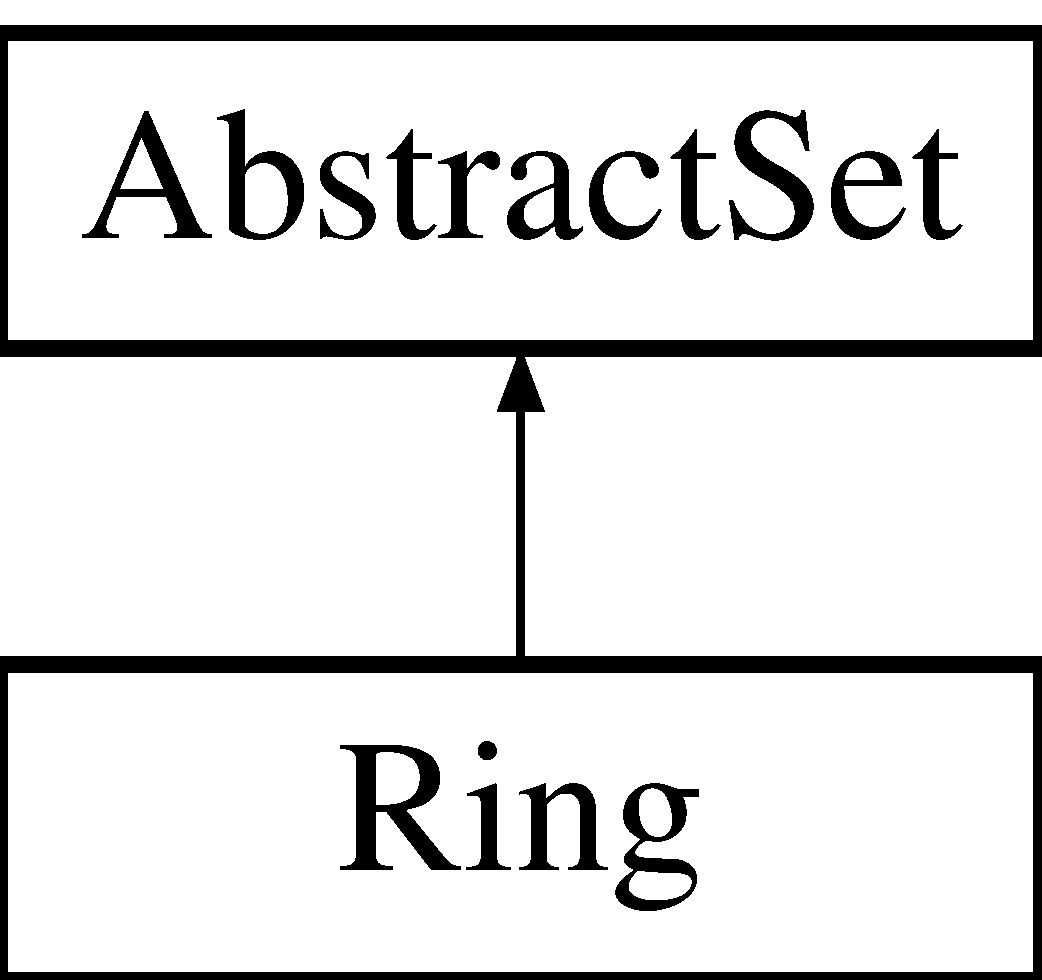
\includegraphics[height=2.000000cm]{classRing}
\end{center}
\end{figure}
\subsection*{Public Member Functions}
\begin{DoxyCompactItemize}
\item 
\hypertarget{classRing_aa2a51e6c57c5073d25f5e077b840feb8}{{\bfseries Ring} (int s)}\label{classRing_aa2a51e6c57c5073d25f5e077b840feb8}

\item 
\hypertarget{classRing_aa311bb3fbd3c7bcca0cca4112d448d40}{int {\bfseries get\-Index} (int i, int j)}\label{classRing_aa311bb3fbd3c7bcca0cca4112d448d40}

\item 
void \hyperlink{classRing_af9bc7f0b325cbd2b6284aadeacdee6fb}{set\-Objective\-Function} (\hyperlink{classObjectiveFunction}{Objective\-Function} $\ast$m)
\begin{DoxyCompactList}\small\item\em Set the objective that one wants to optimise. \end{DoxyCompactList}\item 
\hypertarget{classRing_adc68e6141c7957391e5290749a4bb9c1}{void \hyperlink{classRing_adc68e6141c7957391e5290749a4bb9c1}{set\-Random} ()}\label{classRing_adc68e6141c7957391e5290749a4bb9c1}

\begin{DoxyCompactList}\small\item\em Randomly set the algebraic constraints for quick experiments (warning\-: this method is not always implemented) \end{DoxyCompactList}\item 
\hypertarget{classRing_aecf5e7fe540e174cb718cd167f61c87e}{void \hyperlink{classRing_aecf5e7fe540e174cb718cd167f61c87e}{print} ()}\label{classRing_aecf5e7fe540e174cb718cd167f61c87e}

\begin{DoxyCompactList}\small\item\em Print the set and its algebraic constraints. \end{DoxyCompactList}\item 
\hypertarget{classRing_a263c2e8e2f934f15246b17b60017460b}{void \hyperlink{classRing_a263c2e8e2f934f15246b17b60017460b}{build\-Data\-Structure} ()}\label{classRing_a263c2e8e2f934f15246b17b60017460b}

\begin{DoxyCompactList}\small\item\em Build a proper data structure to represent the set and its algebraic constraints (warning\-: this method should always be called after instantiating and parameterising a set, and before calling any other method, such as \hyperlink{classRing_aecf5e7fe540e174cb718cd167f61c87e}{print()}, \hyperlink{classRing_afe95373425bb2f3c0f0d3cfbea5c96e8}{compute\-Objective\-Values()}, compute\-Optimal\-Partition (double parameter), etc.) \end{DoxyCompactList}\item 
\hypertarget{classRing_afe95373425bb2f3c0f0d3cfbea5c96e8}{void \hyperlink{classRing_afe95373425bb2f3c0f0d3cfbea5c96e8}{compute\-Objective\-Values} ()}\label{classRing_afe95373425bb2f3c0f0d3cfbea5c96e8}

\begin{DoxyCompactList}\small\item\em Compute the value of the objective function for each feasible part (warning\-: set\-Objective\-Function (\hyperlink{classObjectiveFunction}{Objective\-Function} $\ast$objective) should have been called first) \end{DoxyCompactList}\item 
\hypertarget{classRing_a95cc78007a2a9f2b3cfe09b33777d9c8}{void \hyperlink{classRing_a95cc78007a2a9f2b3cfe09b33777d9c8}{normalize\-Objective\-Values} ()}\label{classRing_a95cc78007a2a9f2b3cfe09b33777d9c8}

\begin{DoxyCompactList}\small\item\em Finish computing the value of the objective function for each feasible part when normalisation is required (warning\-: only after \hyperlink{classRing_afe95373425bb2f3c0f0d3cfbea5c96e8}{compute\-Objective\-Values()} has been called) \end{DoxyCompactList}\item 
\hypertarget{classRing_ad61ae2d29f241366efbc67ee3ce3d240}{void \hyperlink{classRing_ad61ae2d29f241366efbc67ee3ce3d240}{print\-Objective\-Values} ()}\label{classRing_ad61ae2d29f241366efbc67ee3ce3d240}

\begin{DoxyCompactList}\small\item\em Print the value of the objective function for each feasible part. \end{DoxyCompactList}\item 
void \hyperlink{classRing_a196b62e9291ed1012ec89f0b2ccd489f}{compute\-Optimal\-Partition} (double parameter)
\begin{DoxyCompactList}\small\item\em Compute a partition that fits with the algebraic constraints and that optimises the objective function that has been specified. \end{DoxyCompactList}\item 
void \hyperlink{classRing_add25abfb4d058b0229a2582913118fcf}{print\-Optimal\-Partition} (double parameter)
\begin{DoxyCompactList}\small\item\em Compute and print a partition that fits with the algebraic constraints and that optimises the objective function that has been specified (warning\-: this method is not always implemented, but one can obtain a similar result by using get\-Optimal\-Partition (double parameter) and by calling \hyperlink{classRing_aecf5e7fe540e174cb718cd167f61c87e}{print()} on the result) \end{DoxyCompactList}\item 
\hyperlink{classPartition}{Partition} $\ast$ \hyperlink{classRing_ac9566fc23a18846375886fed4680b55a}{get\-Optimal\-Partition} (double parameter)
\begin{DoxyCompactList}\small\item\em Compute and return a partition that fits with the algebraic constraints and that optimises the objective function that has been specified (warning\-: this method is not always implemented, but one can obtain a similar result by using get\-Optimal\-Partition (double parameter) and by calling \hyperlink{classRing_aecf5e7fe540e174cb718cd167f61c87e}{print()} on the result) \end{DoxyCompactList}\item 
\hypertarget{classRing_a150f37e6ecbf13f553d9da97034a7ed9}{\hyperlink{classAbstractSet}{Abstract\-Set} $\ast$ {\bfseries get\-Random\-Set} (int size)}\label{classRing_a150f37e6ecbf13f553d9da97034a7ed9}

\end{DoxyCompactItemize}
\subsection*{Public Attributes}
\begin{DoxyCompactItemize}
\item 
\hypertarget{classRing_a9504e0a5404f0fc0a7634e2d10021025}{int {\bfseries size}}\label{classRing_a9504e0a5404f0fc0a7634e2d10021025}

\item 
\hypertarget{classRing_a785645b900755ef5e81633f7122abbe0}{double $\ast$ {\bfseries values}}\label{classRing_a785645b900755ef5e81633f7122abbe0}

\item 
\hypertarget{classRing_aef9d5820742c6251ec52ef9351017cc9}{double $\ast$ {\bfseries sum\-Values}}\label{classRing_aef9d5820742c6251ec52ef9351017cc9}

\item 
\hypertarget{classRing_af55ff3fa2edc4d9b14be1e1bdff07a62}{double $\ast$ {\bfseries micro\-Infos}}\label{classRing_af55ff3fa2edc4d9b14be1e1bdff07a62}

\item 
\hypertarget{classRing_a9c98f90fc9bb2026731ecc45078157de}{double $\ast$ {\bfseries size\-Reductions}}\label{classRing_a9c98f90fc9bb2026731ecc45078157de}

\item 
\hypertarget{classRing_afb390919187938553b890f6ca7ecd9d6}{double $\ast$ {\bfseries divergences}}\label{classRing_afb390919187938553b890f6ca7ecd9d6}

\item 
\hypertarget{classRing_a78f8836d9650b81534b5e903ddb257db}{double $\ast$ {\bfseries optimal\-Qualities}}\label{classRing_a78f8836d9650b81534b5e903ddb257db}

\item 
\hypertarget{classRing_acaa4d3ecf8218e9d28304977389ddd59}{int $\ast$ {\bfseries optimal\-Cuts}}\label{classRing_acaa4d3ecf8218e9d28304977389ddd59}

\item 
\hypertarget{classRing_ae5d182d18fb883761289b7132bc93bd8}{int {\bfseries first\-Optimal\-Cut}}\label{classRing_ae5d182d18fb883761289b7132bc93bd8}

\item 
\hypertarget{classRing_ad846e68433d09f977257148c7ab8514b}{int {\bfseries last\-Optimal\-Cut}}\label{classRing_ad846e68433d09f977257148c7ab8514b}

\end{DoxyCompactItemize}


\subsection{Member Function Documentation}
\hypertarget{classRing_a196b62e9291ed1012ec89f0b2ccd489f}{\index{Ring@{Ring}!compute\-Optimal\-Partition@{compute\-Optimal\-Partition}}
\index{compute\-Optimal\-Partition@{compute\-Optimal\-Partition}!Ring@{Ring}}
\subsubsection[{compute\-Optimal\-Partition}]{\setlength{\rightskip}{0pt plus 5cm}void Ring\-::compute\-Optimal\-Partition (
\begin{DoxyParamCaption}
\item[{double}]{parameter}
\end{DoxyParamCaption}
)\hspace{0.3cm}{\ttfamily [virtual]}}}\label{classRing_a196b62e9291ed1012ec89f0b2ccd489f}


Compute a partition that fits with the algebraic constraints and that optimises the objective function that has been specified. 


\begin{DoxyParams}{Parameters}
{\em parameter} & \-: The parameter of the objective function to be optimised (if the objective is parametrised) \\
\hline
\end{DoxyParams}


Implements \hyperlink{classAbstractSet_acfc3004f18192f38e32bb7a5a12ec8df}{Abstract\-Set}.

\hypertarget{classRing_ac9566fc23a18846375886fed4680b55a}{\index{Ring@{Ring}!get\-Optimal\-Partition@{get\-Optimal\-Partition}}
\index{get\-Optimal\-Partition@{get\-Optimal\-Partition}!Ring@{Ring}}
\subsubsection[{get\-Optimal\-Partition}]{\setlength{\rightskip}{0pt plus 5cm}{\bf Partition} $\ast$ Ring\-::get\-Optimal\-Partition (
\begin{DoxyParamCaption}
\item[{double}]{parameter}
\end{DoxyParamCaption}
)\hspace{0.3cm}{\ttfamily [virtual]}}}\label{classRing_ac9566fc23a18846375886fed4680b55a}


Compute and return a partition that fits with the algebraic constraints and that optimises the objective function that has been specified (warning\-: this method is not always implemented, but one can obtain a similar result by using get\-Optimal\-Partition (double parameter) and by calling \hyperlink{classRing_aecf5e7fe540e174cb718cd167f61c87e}{print()} on the result) 


\begin{DoxyParams}{Parameters}
{\em parameter} & \-: The parameter of the objective function to be optimised (if the objective is parametrised) \\
\hline
\end{DoxyParams}
\begin{DoxyReturn}{Returns}
\-: The resulting optimal partition 
\end{DoxyReturn}


Implements \hyperlink{classAbstractSet_a48fd08c4b61ed46946bed6e19cd11194}{Abstract\-Set}.

\hypertarget{classRing_add25abfb4d058b0229a2582913118fcf}{\index{Ring@{Ring}!print\-Optimal\-Partition@{print\-Optimal\-Partition}}
\index{print\-Optimal\-Partition@{print\-Optimal\-Partition}!Ring@{Ring}}
\subsubsection[{print\-Optimal\-Partition}]{\setlength{\rightskip}{0pt plus 5cm}void Ring\-::print\-Optimal\-Partition (
\begin{DoxyParamCaption}
\item[{double}]{parameter}
\end{DoxyParamCaption}
)\hspace{0.3cm}{\ttfamily [virtual]}}}\label{classRing_add25abfb4d058b0229a2582913118fcf}


Compute and print a partition that fits with the algebraic constraints and that optimises the objective function that has been specified (warning\-: this method is not always implemented, but one can obtain a similar result by using get\-Optimal\-Partition (double parameter) and by calling \hyperlink{classRing_aecf5e7fe540e174cb718cd167f61c87e}{print()} on the result) 


\begin{DoxyParams}{Parameters}
{\em parameter} & \-: The parameter of the objective function to be optimised (if the objective is parametrised) \\
\hline
\end{DoxyParams}


Implements \hyperlink{classAbstractSet_a82a9ce5c2d30690f0d1b83b034e92e1e}{Abstract\-Set}.

\hypertarget{classRing_af9bc7f0b325cbd2b6284aadeacdee6fb}{\index{Ring@{Ring}!set\-Objective\-Function@{set\-Objective\-Function}}
\index{set\-Objective\-Function@{set\-Objective\-Function}!Ring@{Ring}}
\subsubsection[{set\-Objective\-Function}]{\setlength{\rightskip}{0pt plus 5cm}void Ring\-::set\-Objective\-Function (
\begin{DoxyParamCaption}
\item[{{\bf Objective\-Function} $\ast$}]{objective}
\end{DoxyParamCaption}
)\hspace{0.3cm}{\ttfamily [virtual]}}}\label{classRing_af9bc7f0b325cbd2b6284aadeacdee6fb}


Set the objective that one wants to optimise. 


\begin{DoxyParams}{Parameters}
{\em objective} & \-: The objective function itself \\
\hline
\end{DoxyParams}


Implements \hyperlink{classAbstractSet_a7aef71679a18ab7965d1098da15b26c2}{Abstract\-Set}.



The documentation for this class was generated from the following files\-:\begin{DoxyCompactItemize}
\item 
src/ring.\-hpp\item 
src/ring.\-cpp\end{DoxyCompactItemize}

\hypertarget{classRingGraph}{\section{Ring\-Graph Class Reference}
\label{classRingGraph}\index{Ring\-Graph@{Ring\-Graph}}
}
Inheritance diagram for Ring\-Graph\-:\begin{figure}[H]
\begin{center}
\leavevmode
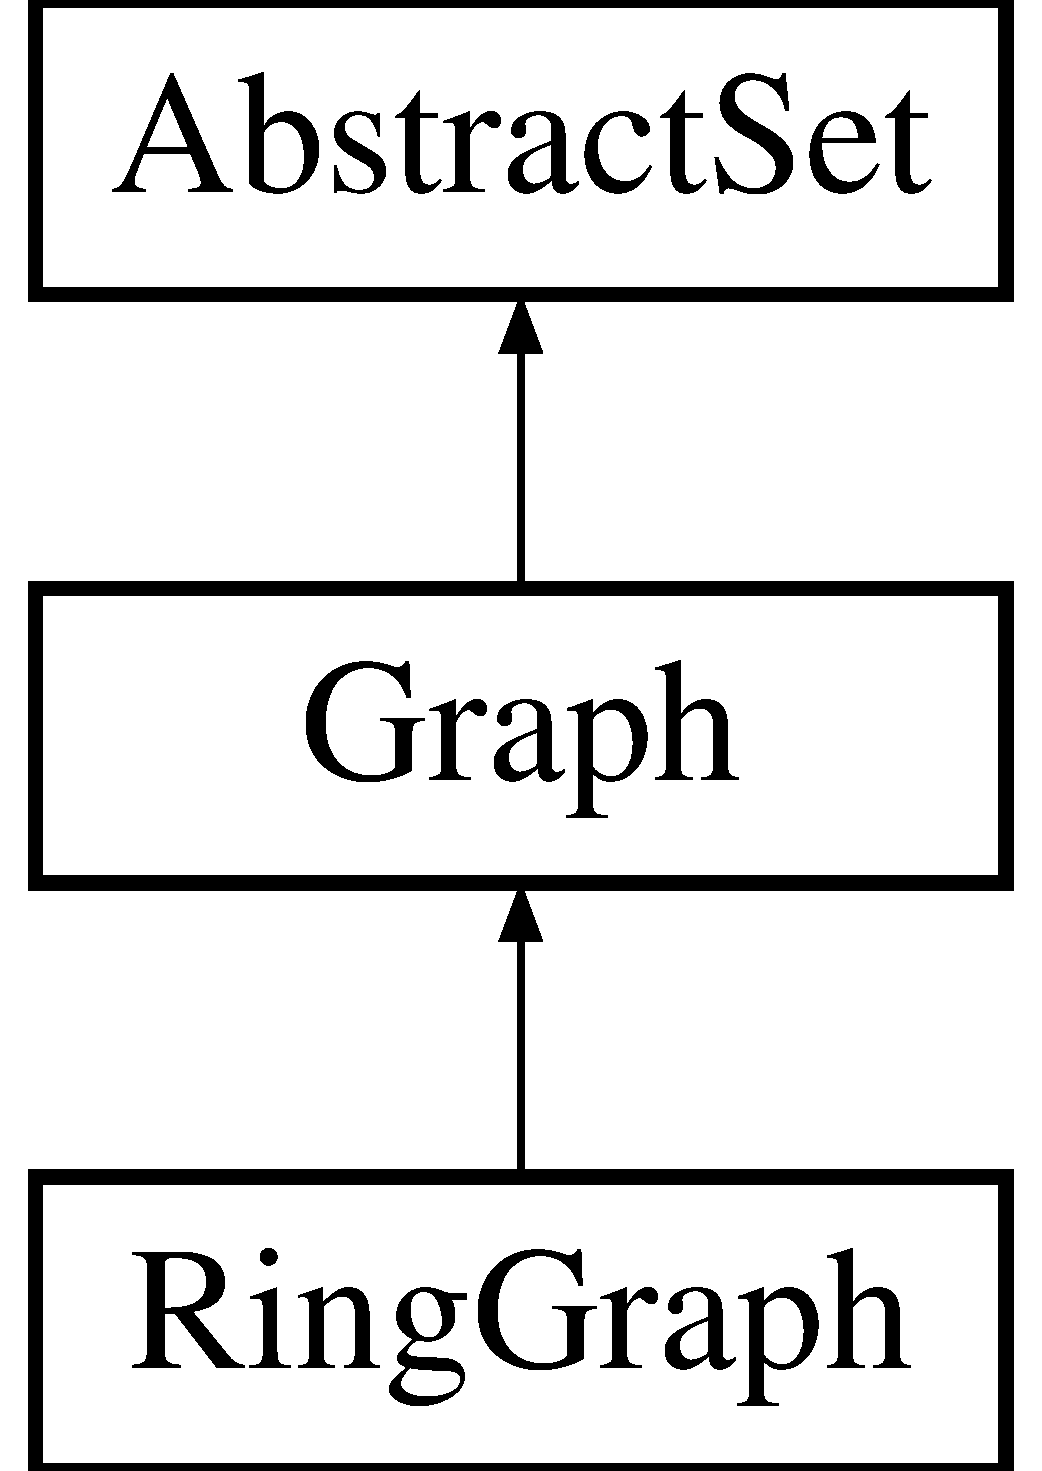
\includegraphics[height=3.000000cm]{classRingGraph}
\end{center}
\end{figure}
\subsection*{Public Member Functions}
\begin{DoxyCompactItemize}
\item 
\hypertarget{classRingGraph_a352a09a7580038e222dca138aa05a054}{{\bfseries Ring\-Graph} (int v\-Num)}\label{classRingGraph_a352a09a7580038e222dca138aa05a054}

\end{DoxyCompactItemize}
\subsection*{Additional Inherited Members}


The documentation for this class was generated from the following files\-:\begin{DoxyCompactItemize}
\item 
src/graph.\-hpp\item 
src/graph.\-cpp\end{DoxyCompactItemize}

\hypertarget{classStructure}{\section{Structure Class Reference}
\label{classStructure}\index{Structure@{Structure}}
}
Inheritance diagram for Structure\-:\begin{figure}[H]
\begin{center}
\leavevmode
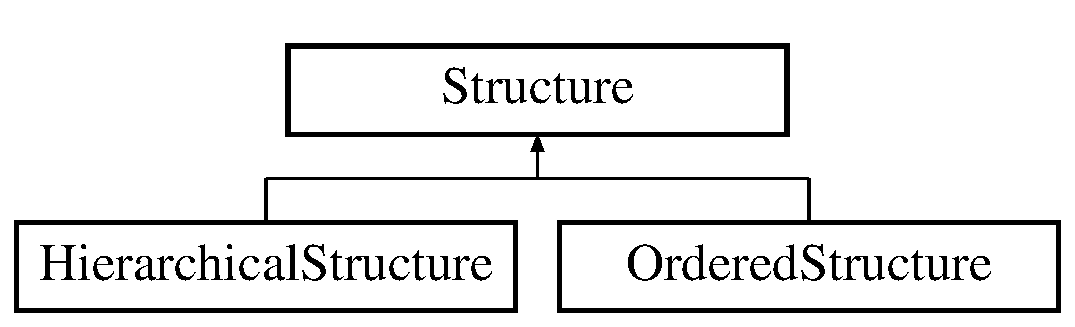
\includegraphics[height=2.000000cm]{classStructure}
\end{center}
\end{figure}
\subsection*{Public Member Functions}
\begin{DoxyCompactItemize}
\item 
\hypertarget{classStructure_ab729d3655c6f8cc57a017990505ca801}{{\bfseries Structure} (\hyperlink{classAggregate}{Aggregate} $\ast$first\-Aggregate)}\label{classStructure_ab729d3655c6f8cc57a017990505ca801}

\item 
\hypertarget{classStructure_a58ba69b728af41d799e311ccfa681ad1}{void {\bfseries build\-Data\-Structure} ()}\label{classStructure_a58ba69b728af41d799e311ccfa681ad1}

\item 
\hypertarget{classStructure_a398196a737f5e5b4bf7e2358531025f0}{void {\bfseries init\-Reached} ()}\label{classStructure_a398196a737f5e5b4bf7e2358531025f0}

\item 
\hypertarget{classStructure_af0552334481ce744845b343590263a46}{void {\bfseries print} ()}\label{classStructure_af0552334481ce744845b343590263a46}

\end{DoxyCompactItemize}
\subsection*{Public Attributes}
\begin{DoxyCompactItemize}
\item 
\hypertarget{classStructure_a682a06309b5ee61c2748cfa647767922}{int {\bfseries aggregate\-Number}}\label{classStructure_a682a06309b5ee61c2748cfa647767922}

\item 
\hypertarget{classStructure_aeefae0ee6589529db98c11daa42a6359}{int {\bfseries atomic\-Aggregate\-Number}}\label{classStructure_aeefae0ee6589529db98c11daa42a6359}

\item 
\hypertarget{classStructure_a5926547e9f7996fbc50dc6d2c95311de}{\hyperlink{classAggregate}{Aggregate} $\ast$ {\bfseries first\-Aggregate}}\label{classStructure_a5926547e9f7996fbc50dc6d2c95311de}

\item 
\hypertarget{classStructure_a3499b465bca65bd0d0e6807bea397837}{\hyperlink{classAggregate}{Aggregate} $\ast$$\ast$ {\bfseries aggregate\-Array}}\label{classStructure_a3499b465bca65bd0d0e6807bea397837}

\item 
\hypertarget{classStructure_aa8f9b7e8ba6f13971ad221bbb61224da}{\hyperlink{classAggregate}{Aggregate} $\ast$$\ast$ {\bfseries atomic\-Aggregate\-Array}}\label{classStructure_aa8f9b7e8ba6f13971ad221bbb61224da}

\end{DoxyCompactItemize}


The documentation for this class was generated from the following files\-:\begin{DoxyCompactItemize}
\item 
/home/lamarche/programming/optimal\-\_\-partition/src/structure.\-hpp\item 
/home/lamarche/programming/optimal\-\_\-partition/src/structure.\-cpp\end{DoxyCompactItemize}

\hypertarget{classStructure2D}{\section{Structure2\-D Class Reference}
\label{classStructure2D}\index{Structure2\-D@{Structure2\-D}}
}
Inheritance diagram for Structure2\-D\-:\begin{figure}[H]
\begin{center}
\leavevmode
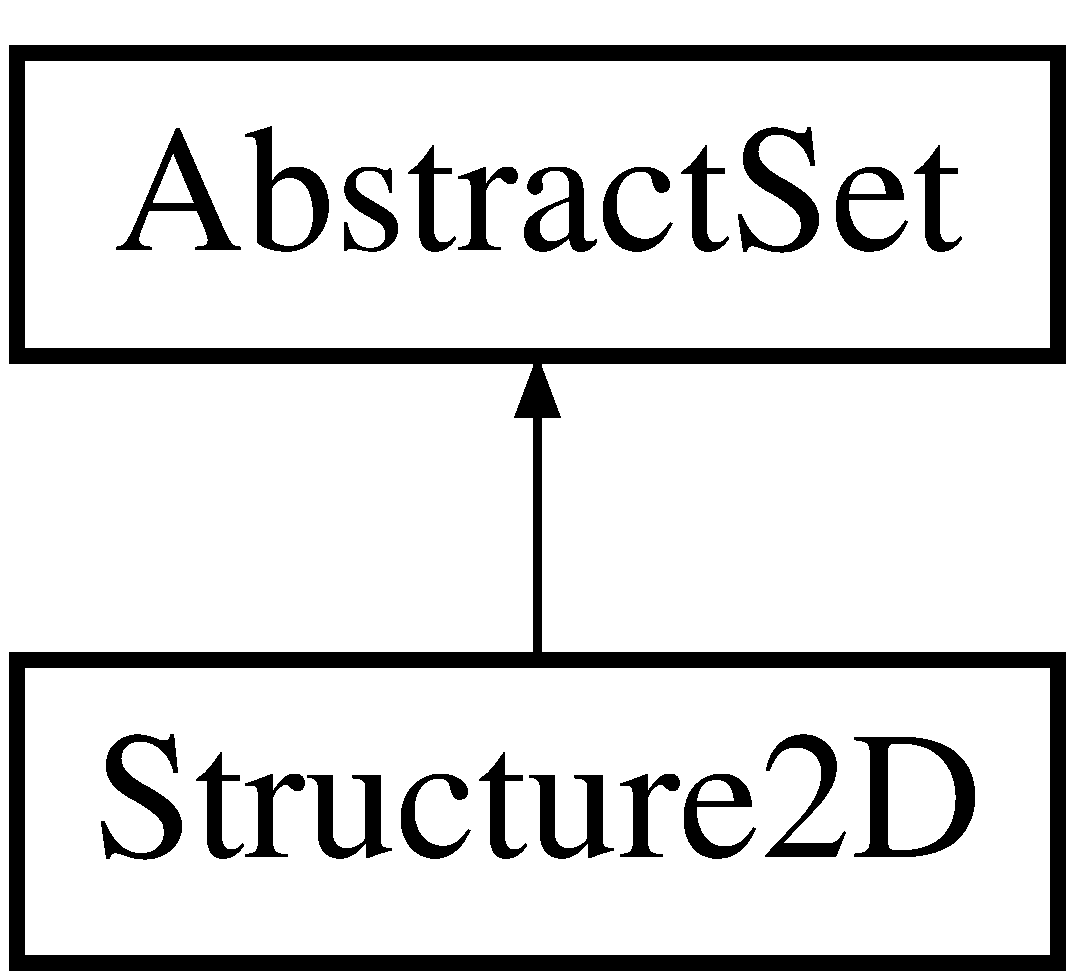
\includegraphics[height=2.000000cm]{classStructure2D}
\end{center}
\end{figure}
\subsection*{Public Member Functions}
\begin{DoxyCompactItemize}
\item 
\hypertarget{classStructure2D_acf11018d9c07b17ae9994a2748a5b595}{{\bfseries Structure2\-D} (\hyperlink{classStructure}{Structure} $\ast$structure1, \hyperlink{classStructure}{Structure} $\ast$structure2)}\label{classStructure2D_acf11018d9c07b17ae9994a2748a5b595}

\item 
\hypertarget{classStructure2D_a7d494335421734e80964f0907f0869d2}{void {\bfseries init\-Reached} ()}\label{classStructure2D_a7d494335421734e80964f0907f0869d2}

\item 
\hypertarget{classStructure2D_a0074288112f5f352f4d5b2f068551ae4}{void \hyperlink{classStructure2D_a0074288112f5f352f4d5b2f068551ae4}{set\-Random} ()}\label{classStructure2D_a0074288112f5f352f4d5b2f068551ae4}

\begin{DoxyCompactList}\small\item\em Randomly set the algebraic constraints for quick experiments (warning\-: this method is not always implemented) \end{DoxyCompactList}\item 
void \hyperlink{classStructure2D_a85e5a4395ec60a75f3bcd1c7cacd6e2c}{set\-Objective\-Function} (\hyperlink{classObjectiveFunction}{Objective\-Function} $\ast$m)
\begin{DoxyCompactList}\small\item\em Set the objective that one wants to optimise. \end{DoxyCompactList}\item 
\hypertarget{classStructure2D_ac51082d3ad73344ea13921dd450d865f}{void \hyperlink{classStructure2D_ac51082d3ad73344ea13921dd450d865f}{print} ()}\label{classStructure2D_ac51082d3ad73344ea13921dd450d865f}

\begin{DoxyCompactList}\small\item\em Print the set and its algebraic constraints. \end{DoxyCompactList}\item 
\hypertarget{classStructure2D_a337047bfc3a936c9e3255e8b4844e734}{void \hyperlink{classStructure2D_a337047bfc3a936c9e3255e8b4844e734}{build\-Data\-Structure} ()}\label{classStructure2D_a337047bfc3a936c9e3255e8b4844e734}

\begin{DoxyCompactList}\small\item\em Build a proper data structure to represent the set and its algebraic constraints (warning\-: this method should always be called after instantiating and parameterising a set, and before calling any other method, such as \hyperlink{classStructure2D_ac51082d3ad73344ea13921dd450d865f}{print()}, \hyperlink{classStructure2D_a9c191ec37069690052006794045b7a72}{compute\-Objective\-Values()}, compute\-Optimal\-Partition (double parameter), etc.) \end{DoxyCompactList}\item 
\hypertarget{classStructure2D_a9c191ec37069690052006794045b7a72}{void \hyperlink{classStructure2D_a9c191ec37069690052006794045b7a72}{compute\-Objective\-Values} ()}\label{classStructure2D_a9c191ec37069690052006794045b7a72}

\begin{DoxyCompactList}\small\item\em Compute the value of the objective function for each feasible part (warning\-: set\-Objective\-Function (\hyperlink{classObjectiveFunction}{Objective\-Function} $\ast$objective) should have been called first) \end{DoxyCompactList}\item 
\hypertarget{classStructure2D_aa1d0292f7eff04ba4381246c778ab843}{void \hyperlink{classStructure2D_aa1d0292f7eff04ba4381246c778ab843}{normalize\-Objective\-Values} ()}\label{classStructure2D_aa1d0292f7eff04ba4381246c778ab843}

\begin{DoxyCompactList}\small\item\em Finish computing the value of the objective function for each feasible part when normalisation is required (warning\-: only after \hyperlink{classStructure2D_a9c191ec37069690052006794045b7a72}{compute\-Objective\-Values()} has been called) \end{DoxyCompactList}\item 
\hypertarget{classStructure2D_adfe22a0de3b19ded04792c3886933448}{void \hyperlink{classStructure2D_adfe22a0de3b19ded04792c3886933448}{print\-Objective\-Values} ()}\label{classStructure2D_adfe22a0de3b19ded04792c3886933448}

\begin{DoxyCompactList}\small\item\em Print the value of the objective function for each feasible part. \end{DoxyCompactList}\item 
void \hyperlink{classStructure2D_ae47a85c274cefe893414a09819b09806}{compute\-Optimal\-Partition} (double parameter)
\begin{DoxyCompactList}\small\item\em Compute a partition that fits with the algebraic constraints and that optimises the objective function that has been specified. \end{DoxyCompactList}\item 
void \hyperlink{classStructure2D_a45157c8978b9b67cd6efc2ea98b22398}{print\-Optimal\-Partition} (double parameter)
\begin{DoxyCompactList}\small\item\em Compute and print a partition that fits with the algebraic constraints and that optimises the objective function that has been specified (warning\-: this method is not always implemented, but one can obtain a similar result by using get\-Optimal\-Partition (double parameter) and by calling \hyperlink{classStructure2D_ac51082d3ad73344ea13921dd450d865f}{print()} on the result) \end{DoxyCompactList}\item 
\hyperlink{classPartition}{Partition} $\ast$ \hyperlink{classStructure2D_a3e4b40f2cf3b59ce3c39eaf75eda09e4}{get\-Optimal\-Partition} (double parameter)
\begin{DoxyCompactList}\small\item\em Compute and return a partition that fits with the algebraic constraints and that optimises the objective function that has been specified (warning\-: this method is not always implemented, but one can obtain a similar result by using get\-Optimal\-Partition (double parameter) and by calling \hyperlink{classStructure2D_ac51082d3ad73344ea13921dd450d865f}{print()} on the result) \end{DoxyCompactList}\end{DoxyCompactItemize}
\subsection*{Public Attributes}
\begin{DoxyCompactItemize}
\item 
\hypertarget{classStructure2D_ae6e35be16cee4391024f90435df4a081}{\hyperlink{classStructure}{Structure} $\ast$ {\bfseries structure1}}\label{classStructure2D_ae6e35be16cee4391024f90435df4a081}

\item 
\hypertarget{classStructure2D_a2454abc684270e0e416248fc59db7169}{\hyperlink{classStructure}{Structure} $\ast$ {\bfseries structure2}}\label{classStructure2D_a2454abc684270e0e416248fc59db7169}

\item 
\hypertarget{classStructure2D_a5802607fe276b9b18c9255d9c3af8696}{int {\bfseries aggregate\-Number}}\label{classStructure2D_a5802607fe276b9b18c9255d9c3af8696}

\item 
\hypertarget{classStructure2D_aa75c1404b8e20b3234a58b5eee9d76d2}{int {\bfseries atomic\-Aggregate\-Number}}\label{classStructure2D_aa75c1404b8e20b3234a58b5eee9d76d2}

\item 
\hypertarget{classStructure2D_aa48fa180714c86f4b51e8fef13ace772}{\hyperlink{classAggregate2D}{Aggregate2\-D} $\ast$ {\bfseries first\-Aggregate}}\label{classStructure2D_aa48fa180714c86f4b51e8fef13ace772}

\item 
\hypertarget{classStructure2D_a2cd160b5bb5b9404bc0d5232ddb94b12}{\hyperlink{classAggregate2D}{Aggregate2\-D} $\ast$$\ast$ {\bfseries aggregate\-Array}}\label{classStructure2D_a2cd160b5bb5b9404bc0d5232ddb94b12}

\end{DoxyCompactItemize}


\subsection{Member Function Documentation}
\hypertarget{classStructure2D_ae47a85c274cefe893414a09819b09806}{\index{Structure2\-D@{Structure2\-D}!compute\-Optimal\-Partition@{compute\-Optimal\-Partition}}
\index{compute\-Optimal\-Partition@{compute\-Optimal\-Partition}!Structure2D@{Structure2\-D}}
\subsubsection[{compute\-Optimal\-Partition}]{\setlength{\rightskip}{0pt plus 5cm}void Structure2\-D\-::compute\-Optimal\-Partition (
\begin{DoxyParamCaption}
\item[{double}]{parameter}
\end{DoxyParamCaption}
)\hspace{0.3cm}{\ttfamily [virtual]}}}\label{classStructure2D_ae47a85c274cefe893414a09819b09806}


Compute a partition that fits with the algebraic constraints and that optimises the objective function that has been specified. 


\begin{DoxyParams}{Parameters}
{\em parameter} & \-: The parameter of the objective function to be optimised (if the objective is parametrised) \\
\hline
\end{DoxyParams}


Implements \hyperlink{classAbstractSet_acfc3004f18192f38e32bb7a5a12ec8df}{Abstract\-Set}.

\hypertarget{classStructure2D_a3e4b40f2cf3b59ce3c39eaf75eda09e4}{\index{Structure2\-D@{Structure2\-D}!get\-Optimal\-Partition@{get\-Optimal\-Partition}}
\index{get\-Optimal\-Partition@{get\-Optimal\-Partition}!Structure2D@{Structure2\-D}}
\subsubsection[{get\-Optimal\-Partition}]{\setlength{\rightskip}{0pt plus 5cm}{\bf Partition} $\ast$ Structure2\-D\-::get\-Optimal\-Partition (
\begin{DoxyParamCaption}
\item[{double}]{parameter}
\end{DoxyParamCaption}
)\hspace{0.3cm}{\ttfamily [virtual]}}}\label{classStructure2D_a3e4b40f2cf3b59ce3c39eaf75eda09e4}


Compute and return a partition that fits with the algebraic constraints and that optimises the objective function that has been specified (warning\-: this method is not always implemented, but one can obtain a similar result by using get\-Optimal\-Partition (double parameter) and by calling \hyperlink{classStructure2D_ac51082d3ad73344ea13921dd450d865f}{print()} on the result) 


\begin{DoxyParams}{Parameters}
{\em parameter} & \-: The parameter of the objective function to be optimised (if the objective is parametrised) \\
\hline
\end{DoxyParams}
\begin{DoxyReturn}{Returns}
\-: The resulting optimal partition 
\end{DoxyReturn}


Implements \hyperlink{classAbstractSet_a48fd08c4b61ed46946bed6e19cd11194}{Abstract\-Set}.

\hypertarget{classStructure2D_a45157c8978b9b67cd6efc2ea98b22398}{\index{Structure2\-D@{Structure2\-D}!print\-Optimal\-Partition@{print\-Optimal\-Partition}}
\index{print\-Optimal\-Partition@{print\-Optimal\-Partition}!Structure2D@{Structure2\-D}}
\subsubsection[{print\-Optimal\-Partition}]{\setlength{\rightskip}{0pt plus 5cm}void Structure2\-D\-::print\-Optimal\-Partition (
\begin{DoxyParamCaption}
\item[{double}]{parameter}
\end{DoxyParamCaption}
)\hspace{0.3cm}{\ttfamily [virtual]}}}\label{classStructure2D_a45157c8978b9b67cd6efc2ea98b22398}


Compute and print a partition that fits with the algebraic constraints and that optimises the objective function that has been specified (warning\-: this method is not always implemented, but one can obtain a similar result by using get\-Optimal\-Partition (double parameter) and by calling \hyperlink{classStructure2D_ac51082d3ad73344ea13921dd450d865f}{print()} on the result) 


\begin{DoxyParams}{Parameters}
{\em parameter} & \-: The parameter of the objective function to be optimised (if the objective is parametrised) \\
\hline
\end{DoxyParams}


Implements \hyperlink{classAbstractSet_a82a9ce5c2d30690f0d1b83b034e92e1e}{Abstract\-Set}.

\hypertarget{classStructure2D_a85e5a4395ec60a75f3bcd1c7cacd6e2c}{\index{Structure2\-D@{Structure2\-D}!set\-Objective\-Function@{set\-Objective\-Function}}
\index{set\-Objective\-Function@{set\-Objective\-Function}!Structure2D@{Structure2\-D}}
\subsubsection[{set\-Objective\-Function}]{\setlength{\rightskip}{0pt plus 5cm}void Structure2\-D\-::set\-Objective\-Function (
\begin{DoxyParamCaption}
\item[{{\bf Objective\-Function} $\ast$}]{objective}
\end{DoxyParamCaption}
)\hspace{0.3cm}{\ttfamily [virtual]}}}\label{classStructure2D_a85e5a4395ec60a75f3bcd1c7cacd6e2c}


Set the objective that one wants to optimise. 


\begin{DoxyParams}{Parameters}
{\em objective} & \-: The objective function itself \\
\hline
\end{DoxyParams}


Implements \hyperlink{classAbstractSet_a7aef71679a18ab7965d1098da15b26c2}{Abstract\-Set}.



The documentation for this class was generated from the following files\-:\begin{DoxyCompactItemize}
\item 
/home/lamarche/programming/optimal\-\_\-partition/src/structure2\-D.\-hpp\item 
/home/lamarche/programming/optimal\-\_\-partition/src/structure2\-D.\-cpp\end{DoxyCompactItemize}

\hypertarget{classTimer}{\section{Timer Class Reference}
\label{classTimer}\index{Timer@{Timer}}
}
\subsection*{Public Member Functions}
\begin{DoxyCompactItemize}
\item 
\hypertarget{classTimer_a098158b611784dcc5018375b302483a8}{{\bfseries Timer} (char $\ast$file=0, int dimension=1, bool append=false)}\label{classTimer_a098158b611784dcc5018375b302483a8}

\item 
\hypertarget{classTimer_acc61f0c4f2c1e26ba0bb62d367f0977e}{void {\bfseries start} (int size, std\-::string text=\char`\"{}\char`\"{})}\label{classTimer_acc61f0c4f2c1e26ba0bb62d367f0977e}

\item 
\hypertarget{classTimer_a7a3752e22180b31454af4f37a8fee225}{void {\bfseries start} (std\-::vector$<$ int $>$ parameters, std\-::string text=\char`\"{}\char`\"{})}\label{classTimer_a7a3752e22180b31454af4f37a8fee225}

\item 
\hypertarget{classTimer_a5771baafd265be353ab78a4bb77329f9}{void {\bfseries start\-Time} ()}\label{classTimer_a5771baafd265be353ab78a4bb77329f9}

\item 
\hypertarget{classTimer_afada34fd58fb4729b9a6ee7a445f5133}{void {\bfseries start\-Memory} ()}\label{classTimer_afada34fd58fb4729b9a6ee7a445f5133}

\item 
\hypertarget{classTimer_afc259e85201ab94f291b36ed97dbd5e2}{void {\bfseries stop} (std\-::string text=\char`\"{}\char`\"{})}\label{classTimer_afc259e85201ab94f291b36ed97dbd5e2}

\item 
\hypertarget{classTimer_a71c4bba47ccad8ed4131922d1cd6d689}{void {\bfseries stop\-Time} ()}\label{classTimer_a71c4bba47ccad8ed4131922d1cd6d689}

\item 
\hypertarget{classTimer_a55ad7a96c2e75c4a1a7209c8eb89ee9d}{void {\bfseries stop\-Memory} ()}\label{classTimer_a55ad7a96c2e75c4a1a7209c8eb89ee9d}

\item 
\hypertarget{classTimer_a88fa29d9f2422df0ad2ed43b1c28cc04}{void {\bfseries step} (std\-::string text=\char`\"{}\char`\"{})}\label{classTimer_a88fa29d9f2422df0ad2ed43b1c28cc04}

\item 
\hypertarget{classTimer_af29968e93e56c8bf1de7c9f559dfae23}{void {\bfseries print} (char $\ast$f\-Name)}\label{classTimer_af29968e93e56c8bf1de7c9f559dfae23}

\end{DoxyCompactItemize}
\subsection*{Public Attributes}
\begin{DoxyCompactItemize}
\item 
\hypertarget{classTimer_a6c45df1d084a18e41e3a35f6a43df0be}{float {\bfseries time}}\label{classTimer_a6c45df1d084a18e41e3a35f6a43df0be}

\item 
\hypertarget{classTimer_adbb859c7553e9986b41fe6ca0dee1913}{int {\bfseries memory}}\label{classTimer_adbb859c7553e9986b41fe6ca0dee1913}

\end{DoxyCompactItemize}


The documentation for this class was generated from the following files\-:\begin{DoxyCompactItemize}
\item 
/home/lamarche/programming/optimal\-\_\-partition/src/timer.\-hpp\item 
/home/lamarche/programming/optimal\-\_\-partition/src/timer.\-cpp\end{DoxyCompactItemize}

\hypertarget{structTreeToAdd}{\section{Tree\-To\-Add Struct Reference}
\label{structTreeToAdd}\index{Tree\-To\-Add@{Tree\-To\-Add}}
}
\subsection*{Public Attributes}
\begin{DoxyCompactItemize}
\item 
\hypertarget{structTreeToAdd_abebc54c95ff5f9c39b5c888c48e20cc7}{\hyperlink{classDatatree}{Datatree} $\ast$ {\bfseries node}}\label{structTreeToAdd_abebc54c95ff5f9c39b5c888c48e20cc7}

\item 
\hypertarget{structTreeToAdd_aa77d6e9cc086cdda22594aa24cdcf747}{\hyperlink{classDatatree}{Datatree} $\ast$ {\bfseries node\-To\-Add}}\label{structTreeToAdd_aa77d6e9cc086cdda22594aa24cdcf747}

\item 
\hypertarget{structTreeToAdd_a5c6876f0c789a47f670096f88bbd4daf}{Vertices $\ast$ {\bfseries vertices}}\label{structTreeToAdd_a5c6876f0c789a47f670096f88bbd4daf}

\item 
\hypertarget{structTreeToAdd_ac68944fc8f68753e3088ae9d2110ca92}{Vertices $\ast$ {\bfseries adj\-Vertices}}\label{structTreeToAdd_ac68944fc8f68753e3088ae9d2110ca92}

\end{DoxyCompactItemize}


The documentation for this struct was generated from the following file\-:\begin{DoxyCompactItemize}
\item 
src/graph.\-cpp\end{DoxyCompactItemize}

\chapter{File Documentation}
\hypertarget{abstract__set_8hpp}{\section{src/abstract\-\_\-set.hpp File Reference}
\label{abstract__set_8hpp}\index{src/abstract\-\_\-set.\-hpp@{src/abstract\-\_\-set.\-hpp}}
}


Abstract class defining a set of elements that one wants to partition while optimising some (decomposable) objective and preserving some algebraic constraints (set of feasible parts)  


{\ttfamily \#include \char`\"{}timer.\-hpp\char`\"{}}\\*
{\ttfamily \#include \char`\"{}objective\-\_\-function.\-hpp\char`\"{}}\\*
{\ttfamily \#include \char`\"{}partition.\-hpp\char`\"{}}\\*
{\ttfamily \#include \char`\"{}dataset.\-hpp\char`\"{}}\\*
\subsection*{Classes}
\begin{DoxyCompactItemize}
\item 
class \hyperlink{classAbstractSet}{Abstract\-Set}
\begin{DoxyCompactList}\small\item\em Abstract class defining a set of elements that one wants to partition while optimising some (decomposable) objective and preserving some algebraic constraints (set of feasible parts) \end{DoxyCompactList}\end{DoxyCompactItemize}


\subsection{Detailed Description}
Abstract class defining a set of elements that one wants to partition while optimising some (decomposable) objective and preserving some algebraic constraints (set of feasible parts) \begin{DoxyAuthor}{Author}
Robin Lamarche-\/\-Perrin 
\end{DoxyAuthor}
\begin{DoxyDate}{Date}
06/11/2015 
\end{DoxyDate}

%--- End generated contents ---

% Index
\newpage
\phantomsection
\addcontentsline{toc}{chapter}{Index}
\printindex

\end{document}
